% !TEX program = xelatex
% !TEX root = main.tex
\documentclass[11pt,a4paper,fontset=fandol]{ctexart}

\newcommand{\coursecode}{量子力学}
\newcommand{\coursetitle}{Shankar 教材学习笔记}
\newcommand{\academicyear}{2026}

\usepackage[margin=25mm]{geometry}
\usepackage{amsmath,amssymb,amsthm,bm,mathtools}
\usepackage{booktabs,tabularx}
\usepackage{enumitem}
\usepackage{graphicx}
\usepackage{xcolor}
\usepackage{tikz}
\usepackage{fancyhdr}
\usepackage{hyperref}
\usepackage[nameinlink,noabbrev]{cleveref}
\usetikzlibrary{arrows.meta,calc,fit,positioning}

\definecolor{accentRed}{HTML}{D71440}
\definecolor{noteBlue}{HTML}{1F4E79}
\definecolor{verifyOrange}{HTML}{A64B00}

\hypersetup{
  colorlinks=true,
  linkcolor=noteBlue,
  citecolor=noteBlue,
  urlcolor=noteBlue,
  pdftitle={\coursecode：\coursetitle},
  pdfsubject={\academicyear\ 教材学习笔记}
}

\setlength{\parindent}{0pt}
\setlength{\parskip}{0.6em}
\setlist{itemsep=0.25em,topsep=0.35em}
\graphicspath{{figures/}}

\pagestyle{fancy}
\fancyhf{}
\lhead{\coursecode}
\rhead{\coursetitle}
\cfoot{\thepage}
\setlength{\headheight}{14pt}

\newtheorem{definition}{定义}[section]
\newtheorem{theorem}[definition]{定理}
\newtheorem{proposition}[definition]{命题}
\newtheorem{example}[definition]{例}
\newtheorem{remark}[definition]{说明}

\newcommand{\recordid}[1]{%
  \textcolor{noteBlue}{\textbf{编号：}\texttt{#1}}%
}

\newcommand{\studymeta}[5]{%
  \begin{center}
    \begin{tabularx}{\textwidth}{@{}lX@{}}
      \toprule
      学习单元 & \texttt{#1} \\
      学习日期 & #2 \\
      主要资料 & #3 \\
      覆盖范围 & #4 \\
      人工确认 & #5 \\
      \bottomrule
    \end{tabularx}
  \end{center}
}

\newcommand{\exercisemeta}[5]{%
  \begin{center}
    \begin{tabularx}{\textwidth}{@{}lX@{}}
      \toprule
      题组编号 & \texttt{#1} \\
      对应日期 & #2 \\
      主要来源 & #3 \\
      核对状态 & #4 \\
      人工确认 & #5 \\
      \bottomrule
    \end{tabularx}
  \end{center}
}

\newcommand{\notetopic}[2]{%
  \subsection{#2}\label{topic:#1}%
  \recordid{#1}\par
}

\newcommand{\exercisequestion}[2]{%
  \subsection{#2}\label{exercise:#1}%
  \recordid{#1}\par
}

\newcommand{\relatedtopic}[2]{%
  \hyperref[topic:#1]{#2}~(\texttt{#1})%
}

\newcommand{\relatedexercise}[2]{%
  \hyperref[exercise:#1]{#2}~(\texttt{#1})%
}

\newcommand{\verify}[1]{%
  \textcolor{verifyOrange}{\textbf{[待核对：}#1\textbf{]}}%
}

\newcommand{\keyidea}[1]{%
  \par\textcolor{noteBlue}{\textbf{核心。}}#1\par
}

\newcommand{\dialoguesupplement}[1]{%
  \par\textcolor{noteBlue}{\textbf{对话补充。}}#1\par
}

\newenvironment{checkedsolution}
  {\par\textbf{核对后的解答。}\par}
  {\hfill$\square$\par}

\title{\textcolor{accentRed}{\coursecode}\\[0.4em]\coursetitle}
\author{课程学习笔记}
\date{\academicyear}

\newcommand{\ii}{\mathrm{i}}
\newcommand{\ee}{\mathrm{e}}
\newcommand{\dd}{\mathop{}\!\mathrm{d}}

\newcommand{\hilbert}{\mathcal{H}}
\newcommand{\complex}{\mathbb{C}}
\newcommand{\real}{\mathbb{R}}

\newcommand{\ket}[1]{\left|#1\right\rangle}
\newcommand{\bra}[1]{\left\langle #1\right|}
\newcommand{\braket}[2]{\left\langle #1 \middle| #2 \right\rangle}
\newcommand{\ketbra}[2]{\left|#1\right\rangle\!\left\langle #2\right|}
\newcommand{\expect}[1]{\left\langle #1 \right\rangle}

\newcommand{\op}[1]{\hat{#1}}
\newcommand{\comm}[2]{\left[#1,#2\right]}
\newcommand{\anticomm}[2]{\left\{#1,#2\right\}}
\newcommand{\abs}[1]{\left|#1\right|}
\newcommand{\norm}[1]{\left\lVert #1 \right\rVert}
\newcommand{\pdv}[2]{\frac{\partial #1}{\partial #2}}
\newcommand{\odv}[2]{\frac{\dd #1}{\dd #2}}

\DeclareMathOperator{\Tr}{Tr}
\DeclareMathOperator{\Var}{Var}
\DeclareMathOperator{\diag}{diag}


\begin{document}
\maketitle
\begingroup
\setlength{\parskip}{0pt}
\tableofcontents
\endgroup
\clearpage

\section*{学习地图}
\addcontentsline{toc}{section}{学习地图}

\textbf{第 1、2 章}

\begin{center}
\footnotesize
\renewcommand{\arraystretch}{1.0}
\begin{tabularx}{\textwidth}{@{}>{\raggedright\arraybackslash}p{2.7cm}>{\raggedright\arraybackslash}p{4.1cm}>{\raggedright\arraybackslash}p{3.0cm}X@{}}
  \toprule
  单元 & 教材范围 & 学习日期 & 状态 \\
  \midrule
  \hyperref[section:QM-C01-S01]{QM-C01-S01} & 第 1 章 \S 1.1；印刷页 pp.~1--7；PDF pp.~15--21 & 2026-08-17 & 讲解、练习与收口检查完成 \\
  \hyperref[section:QM-C01-S02]{QM-C01-S02} & 第 1 章 \S 1.2；印刷页 pp.~7--11；PDF pp.~21--25 & 2026-08-18 & 讲解、同书练习与收口检查完成 \\
  \hyperref[section:QM-C01-S03]{QM-C01-S03} & 第 1 章 \S 1.3；印刷页 pp.~11--17；PDF pp.~25--31 & 2026-08-19 & 讲解、教材练习与收口检查完成 \\
  \hyperref[section:QM-C01-S04]{QM-C01-S04} & 第 1 章 \S 1.4；印刷页 pp.~17--18；PDF pp.~31--32 & 2026-08-20 & 讲解、教材练习与收口检查完成 \\
  \hyperref[section:QM-C01-S05]{QM-C01-S05} & 第 1 章 \S 1.5；印刷页 pp.~18--20；PDF pp.~32--34 & 2026-08-21 & 讲解、教材例子与自编收口检查完成 \\
  \hyperref[section:QM-C01-S06]{QM-C01-S06} & 第 1 章 \S 1.6；印刷页 pp.~20--29；PDF pp.~34--43 & 2026-08-22 & 讲解、教材习题与收口检查完成 \\
  \hyperref[section:QM-C01-S07]{QM-C01-S07} & 第 1 章 \S 1.7；印刷页 pp.~29--30；PDF pp.~43--44 & 2026-08-23 & 讲解、教材习题与收口检查完成 \\
  \hyperref[section:QM-C01-S08]{QM-C01-S08} & 第 1 章 \S 1.8；印刷页 pp.~30--54；PDF pp.~44--68 & 2026-08-24 至 2026-08-25 & 讲解、代表题与收口检查完成 \\
  \hyperref[section:QM-C01-S09]{QM-C01-S09} & 第 1 章 \S 1.9；印刷页 pp.~54--57；PDF pp.~68--71 & 2026-08-26 & 讲解、教材习题与收口检查完成 \\
  \hyperref[section:QM-C01-S10]{QM-C01-S10} & 第 1 章 \S 1.10；印刷页 pp.~57--73；PDF pp.~71--87 & 2026-08-26 至 2026-08-27 & 讲解、教材例题、习题与收口检查完成 \\
  \hyperref[section:QM-C02-S01]{QM-C02-S01} & 第 2 章 \S 2.1；印刷页 pp.~75--83；PDF pp.~88--96 & 2026-08-27 & 讲解、教材例题、习题与收口检查完成 \\
  \hyperref[section:QM-C02-S02]{QM-C02-S02} & 第 2 章 \S 2.2；印刷页 pp.~83--84；PDF pp.~96--97 & 2026-08-28 & 讲解、自编检验题与收口检查完成 \\
  \hyperref[section:QM-C02-S03]{QM-C02-S03} & 第 2 章 \S 2.3；印刷页 pp.~85--86；PDF pp.~98--99 & 2026-08-29 & 讲解、教材习题与收口检查完成 \\
  \hyperref[section:QM-C02-S04]{QM-C02-S04} & 第 2 章 \S 2.4；印刷页 p.~86；PDF p.~99 & 2026-08-30 & 讲解、自编检验题与收口检查完成 \\
  \hyperref[section:QM-C02-S05]{QM-C02-S05} & 第 2 章 \S 2.5；印刷页 pp.~86--90；PDF pp.~99--103 & 2026-08-31 & 讲解、教材例题、习题与收口检查完成 \\
  \hyperref[section:QM-C02-S06]{QM-C02-S06} & 第 2 章 \S 2.6；印刷页 pp.~90--91；PDF pp.~103--104 & 2026-09-01 & 讲解、自编检验题与收口检查完成 \\
  \hyperref[section:QM-C02-S07]{QM-C02-S07} & 第 2 章 \S 2.7；印刷页 pp.~91--98；PDF pp.~104--111 & 2026-09-02 & 讲解、教材习题与收口检查完成 \\
  \hyperref[section:QM-C02-S08]{QM-C02-S08} & 第 2 章 \S 2.8；印刷页 pp.~98--106；PDF pp.~111--119 & 2026-09-03 & 讲解、教材习题与收口检查完成 \\
  \bottomrule
\end{tabularx}
\end{center}

\textbf{主要教材：}Shankar, \textit{Principles of Quantum Mechanics}。

\textbf{记录规则：}区分教材内容、对话补充及自编题；解答见独立习题部分。

\clearpage
\section*{学习地图（续：第 3 至 7 章）}

\begin{center}
\footnotesize
\renewcommand{\arraystretch}{0.9}
\begin{tabularx}{\textwidth}{@{}>{\raggedright\arraybackslash}p{2.7cm}>{\raggedright\arraybackslash}p{4.1cm}>{\raggedright\arraybackslash}p{3.0cm}X@{}}
  \toprule
  单元 & 教材范围 & 学习日期 & 状态 \\
  \midrule
  \hyperref[section:QM-C03-S01]{QM-C03-S01} & 第 3 章 \S 3.1；印刷页 pp.~107--108；PDF pp.~120--121 & 2026-09-04 & 讲解、自编检查与订正完成 \\
  \hyperref[section:QM-C03-S02]{QM-C03-S02} & 第 3 章 \S 3.2；印刷页 pp.~108--110；PDF pp.~121--123 & 2026-09-05 & 讲解、自编检查与订正完成 \\
  \hyperref[section:QM-C03-S03]{QM-C03-S03} & 第 3 章 \S 3.3；印刷页 pp.~110--112；PDF pp.~123--125 & 2026-09-06 & 讲解、自编检查与订正完成 \\
  \hyperref[section:QM-C03-S04]{QM-C03-S04} & 第 3 章 \S 3.4；印刷页 p.~112；PDF p.~125 & 2026-09-07 & 讲解、教材估算例与自编检查完成 \\
  \hyperref[section:QM-C03-S05]{QM-C03-S05} & 第 3 章 \S 3.5；印刷页 pp.~112--113；PDF pp.~125--126 & 2026-09-08 & 讲解、自编检查与订正完成 \\
  \hyperref[section:QM-C04-S01]{QM-C04-S01} & 第 4 章 \S 4.1；印刷页 pp.~115--116；PDF pp.~127--128 & 2026-09-08 & 讲解、教材练习 4.2.1 与订正完成 \\
  \hyperref[section:QM-C04-S02]{QM-C04-S02} & 第 4 章 \S 4.2；印刷页 pp.~116--143；PDF pp.~128--155 & 2026-09-10 & 讲解、教材例题与练习 4.2.2--4.2.3 完成 \\
  \hyperref[section:QM-C04-S03]{QM-C04-S03} & 第 4 章 \S 4.3；印刷页 pp.~143--150；PDF pp.~155--162 & 2026-09-11 & 讲解、教材正文推导与应用、自编综合检验完成 \\
  \hyperref[section:QM-C05-S01]{QM-C05-S01} & 第 5 章 \S 5.1；印刷页 pp.~151--157；PDF pp.~163--169 & 2026-09-12 & 讲解、教材练习 5.1.1--5.1.4 与订正完成 \\
  \hyperref[section:QM-C05-S02]{QM-C05-S02} & 第 5 章 \S 5.2；印刷页 pp.~157--164；PDF pp.~169--176 & 2026-09-13 & 讲解、教材练习 5.2.1--5.2.6 与订正完成 \\
  \hyperref[section:QM-C05-S03]{QM-C05-S03} & 第 5 章 \S 5.3；印刷页 pp.~165--167；PDF pp.~177--179 & 2026-09-14 & 讲解、教材练习 5.3.1--5.3.4 与订正完成 \\
  \hyperref[section:QM-C05-S04]{QM-C05-S04} & 第 5 章 \S 5.4；印刷页 pp.~167--175；PDF pp.~179--187 & 2026-09-15 & 讲解、教材练习 5.4.1--5.4.3 与订正完成 \\
  \hyperref[section:QM-C05-S05]{QM-C05-S05} & 第 5 章 \S 5.5；印刷页 pp.~175--176；PDF pp.~187--188 & 2026-09-16 & 讲解、自编短应用题与核对完成 \\
  \hyperref[section:QM-C05-S06]{QM-C05-S06} & 第 5 章 \S 5.6；印刷页 pp.~176--178；PDF pp.~188--190 & 2026-09-17 & 两条定理、教材正文计算检验与核对完成 \\
  \hyperref[section:QM-C06-S01]{QM-C06-S01} & 第 6 章全文；印刷页 pp.~179--184；PDF pp.~191--196 & 2026-09-17 至 2026-09-18 & 讲解与例题完成；笔记已确认 \\
  \hyperref[section:QM-C07-S01]{QM-C07-S01} & 第 7 章 \S 7.1；印刷页 pp.~185--188；PDF pp.~197--200 & 2026-09-19 & 讲解与概念核对完成；笔记待确认 \\
  \bottomrule
\end{tabularx}
\end{center}


\clearpage
\part{教材精讲}
% 教材：Shankar, Principles of Quantum Mechanics
% 精确范围：第 1 章第 1.1 节，印刷页 pp. 1--7，PDF pp. 15--21
% 人工核验：已完成讲解、问答和教材练习 1.1.1--1.1.5

\section{第 1.1 节：线性向量空间基础}
\label{section:QM-C01-S01}

\studymeta
  {QM-C01-S01}
  {2026-08-17}
  {Shankar, \textit{Principles of Quantum Mechanics}}
  {第 1 章 \S 1.1；印刷页 pp.~1--7；PDF pp.~15--21}
  {已确认（讲解、问答与教材练习核验）}

\subsection{本节主线}

线性向量空间把箭头、矩阵、函数等外形不同的对象统一起来。统一它们的不是长度和方向，而是两种运算：向量加法与标量数乘。公理确定哪些推理对所有向量空间都成立；线性无关、维数和基进一步说明如何用一组坐标唯一表示抽象向量。

\notetopic{QM-C01-S01-T01}{向量空间、标量域与公理}

\keyidea{“向量”首先是向量空间中的元素，不一定是箭头或一列数。判断一个集合是否为向量空间，要先说明允许的标量以及向量加法、标量数乘的规则。}

\begin{definition}
设 $V$ 是一个集合，标量来自数域 $\mathbb{F}$。若 $V$ 上定义了向量加法与标量数乘，并满足下列条件，则称 $V$ 为 $\mathbb{F}$ 上的线性向量空间：
\begin{enumerate}
  \item 对任意 $\ket{V},\ket{W}\in V$，有 $\ket{V}+\ket{W}\in V$；对任意 $a\in\mathbb{F}$，有 $a\ket{V}\in V$；
  \item $\ket{V}+\ket{W}=\ket{W}+\ket{V}$；
  \item $\ket{V}+(\ket{W}+\ket{Z})=(\ket{V}+\ket{W})+\ket{Z}$；
  \item 存在唯一的零向量 $\ket{0}$，使 $\ket{V}+\ket{0}=\ket{V}$；
  \item 每个 $\ket{V}$ 都有加法逆元 $-\ket{V}$，使 $\ket{V}+(-\ket{V})=\ket{0}$；
  \item $a(\ket{V}+\ket{W})=a\ket{V}+a\ket{W}$；
  \item $(a+b)\ket{V}=a\ket{V}+b\ket{V}$；
  \item $a(b\ket{V})=(ab)\ket{V}$，且 $1\ket{V}=\ket{V}$。
\end{enumerate}
\end{definition}

数域决定允许使用的标量。$\mathbb{F}=\real$ 时称为实向量空间，$\mathbb{F}=\complex$ 时称为复向量空间；“实”或“复”修饰的是标量，不要求向量对象本身看起来像实数或复数。

\begin{remark}
教材此处列出的公理没有单独写出 $1\ket{V}=\ket{V}$。本笔记按标准线性代数定义将标量单位元作用写明；后续涉及坐标和基时默认采用这一标准条件。
\end{remark}

由公理可以推出：零向量唯一，$0\ket{V}=\ket{0}$，$(-1)\ket{V}=-\ket{V}$，并且每个向量的加法逆元唯一。完整证明见\relatedexercise{QM-C01-S01-E01}{教材练习 1.1.1}。

\notetopic{QM-C01-S01-T02}{典型例子、封闭性与齐次约束}

箭头在通常的首尾相接加法和实数伸缩下构成实向量空间，但只取 $z$ 分量为正的箭头不构成向量空间：零向量不在集合中，负数数乘和加法逆元也会离开集合。

所有 $2\times 2$ 实矩阵在逐项相加与实数数乘下构成向量空间。零向量是零矩阵，加法逆元由每个矩阵元取负得到。矩阵在这里是“向量空间的元素”；矩阵乘法不是定义该向量空间所必需的运算。

区间 $0\leq x\leq L$ 上的函数在逐点相加和数乘下也可构成向量空间。例如，满足
\[
  f(0)=f(L)=0
\]
或
\[
  f(0)=f(L)
\]
的函数集合都对加法和数乘封闭，并包含零函数与加法逆函数。相反，满足 $f(0)=4$ 的函数集合不包含零函数，且一般不对加法、数乘和取负封闭。

\dialoguesupplement{形如 $L(f)=0$ 的齐次线性约束通常定义一个向量子空间；形如 $L(f)=c\neq0$ 的非齐次约束通常不构成向量空间。这是快速判断规则，最终仍须检查零向量和两种封闭性。}

\notetopic{QM-C01-S01-T03}{线性组合、线性相关与线性无关}

\begin{definition}
对向量组 $\ket{1},\ldots,\ket{n}$，表达式
\[
  \sum_{i=1}^{n}a_i\ket{i}=\ket{0}
\]
称为一条线性关系。若它只有平凡解 $a_1=\cdots=a_n=0$，该向量组线性无关；若存在不全为零的系数使等式成立，该向量组线性相关。
\end{definition}

若一条非平凡线性关系中 $a_k\neq0$，则
\[
  \ket{k}=-\sum_{i\neq k}\frac{a_i}{a_k}\ket{i}.
\]
因此线性相关等价于至少有一个向量可以由其余向量线性表示。证明线性相关只需找到一个非平凡关系；证明线性无关则必须排除所有非平凡关系。

平面内两个不平行的非零箭头线性无关，而任意三个平面箭头都线性相关。教材练习中的矩阵关系
\[
  \ket{1}-2\ket{2}=\ket{3}
\]
也直接给出非平凡线性关系，见\relatedexercise{QM-C01-S01-E04}{教材练习 1.1.4}。

\notetopic{QM-C01-S01-T04}{维数、基与展开定理}

\begin{definition}
一个向量空间能够容纳的线性无关向量的最大数目称为该空间的维数。若最大数目为 $n$，则该空间是 $n$ 维的。
\end{definition}

维数依赖标量域。例如 $\complex$ 作为复向量空间的维数为 $1$，基可取 $\{1\}$；作为实向量空间的维数为 $2$，基可取 $\{1,\ii\}$。

\begin{theorem}
在 $n$ 维向量空间中，任意 $n$ 个线性无关向量都能张成整个空间。
\end{theorem}

\textbf{证明。}设 $\ket{1},\ldots,\ket{n}$ 线性无关。若存在 $\ket{V}$ 不能由它们线性表示，则 $\ket{1},\ldots,\ket{n},\ket{V}$ 仍然线性无关：在线性关系
\[
  a\ket{V}+\sum_{i=1}^{n}b_i\ket{i}=\ket{0}
\]
中，若 $a\neq0$，就能解出 $\ket{V}$ 是其余向量的线性组合，与假设矛盾；故 $a=0$，再由原向量组线性无关得到全部 $b_i=0$。这将产生 $n+1$ 个线性无关向量，与空间为 $n$ 维矛盾。因此任意 $\ket{V}$ 都在这 $n$ 个向量的张成空间中。\hfill$\square$

\begin{definition}
一组既线性无关又张成整个空间的向量称为一组基。在已知空间为 $n$ 维时，这等价于取 $n$ 个线性无关向量。
\end{definition}

于是任意向量都可以写为
\begin{equation}
  \ket{V}=\sum_{i=1}^{n}v_i\ket{i},
  \label{eq:QM-C01-S01-basis-expansion}
\end{equation}
其中 $\{\ket{i}\}_{i=1}^{n}$ 是一组基，$v_i$ 称为 $\ket{V}$ 在该基下的分量或坐标。

\notetopic{QM-C01-S01-T05}{坐标唯一性与换基}

\begin{theorem}
同一个向量在给定的一组基下具有唯一的坐标。
\end{theorem}

\textbf{证明。}若
\[
  \ket{V}=\sum_i v_i\ket{i}=\sum_i v_i'\ket{i},
\]
则相减得到
\[
  \sum_i(v_i-v_i')\ket{i}=\ket{0}.
\]
基向量线性无关，所以每个系数差都必须为零，即 $v_i=v_i'$。\hfill$\square$

唯一性中的“给定一组基”不可省略。更换基以后，坐标通常改变，但抽象向量本身不变。例如若
\[
  \ket{1'}=\ket{1}+\ket{2},\qquad
  \ket{2'}=\ket{1}-\ket{2},
\]
则同一个向量可以写成
\[
  \ket{V}=3\ket{1}-2\ket{2}
  =\frac{1}{2}\ket{1'}+\frac{5}{2}\ket{2'}.
\]
第二个表达式可通过展开新基并比较 $\ket{1},\ket{2}$ 的系数验证。

若
\[
  \ket{V}=\sum_i v_i\ket{i},\qquad
  \ket{W}=\sum_i w_i\ket{i},
\]
则
\[
  \ket{V}+\ket{W}=\sum_i(v_i+w_i)\ket{i},\qquad
  a\ket{V}=\sum_i(av_i)\ket{i}.
\]
所以选定基以后，抽象的向量运算转化为对应分量的普通运算。

\notetopic{QM-C01-S01-T06}{矩阵与函数的坐标表示：对话补充}

任意实 $2\times2$ 矩阵都可唯一写成
\[
  \begin{pmatrix}a&b\\c&d\end{pmatrix}
  =a\begin{pmatrix}1&0\\0&0\end{pmatrix}
  +b\begin{pmatrix}0&1\\0&0\end{pmatrix}
  +c\begin{pmatrix}0&0\\1&0\end{pmatrix}
  +d\begin{pmatrix}0&0\\0&1\end{pmatrix}.
\]
因此 $M_{2\times2}(\real)$ 与 $\real^4$ 作为向量空间同构，矩阵的坐标可写成 $(a,b,c,d)^{\mathsf T}$。保留矩阵形式的好处是能够直接看出行列结构，并自然表达矩阵乘法、线性映射复合和特征值等额外结构。

有限维函数空间同样可以坐标化。例如
\[
  P_2=\{a+bx+cx^2:a,b,c\in\real\}
\]
在基 $\{1,x,x^2\}$ 下与 $\real^3$ 同构。一般函数空间可能是无限维的；只记录有限个采样值通常会丢失信息，除非事先限制函数类别。保留函数形式则便于表达连续变量、微分、积分和边界条件。

\begin{remark}
本知识点是学习对话中的补充解释，不是教材第 1.1 节的独立定理。其作用是连接“抽象向量”与熟悉的坐标列向量；无限维空间的严格坐标展开需要后续的内积与完备性概念。
\end{remark}

\subsection{一分钟回顾}

向量空间由标量域、向量加法、标量数乘和相应公理确定。线性无关意味着不存在非平凡的零向量线性关系；维数是线性无关向量数目的上限；基同时具备线性无关和张成性质。给定基后，每个向量具有唯一坐标，向量加法和标量数乘可逐分量进行。矩阵和函数都可以是向量，列数组只是选定基之后的坐标表达。

\section{第 2.1 节：最小作用量原理与拉格朗日力学}
\label{section:QM-C02-S01}

\studymeta
  {QM-C02-S01}
  {2026-08-27}
  {Shankar, \textit{Principles of Quantum Mechanics}, Second Edition}
  {第 2 章 \S 2.1；印刷页 pp.~75--83；PDF pp.~88--96}
  {内容、教材例题与练习 2.1.1--2.1.3 已核对}

\subsection{本节主线}

Newton 力学从某一时刻的位置与速度出发，用局部微分方程逐步确定轨迹；Lagrange 力学则给连接固定时空端点的每条候选路径分配作用量，并以作用量的一阶变分为零选出经典路径。变分计算产生 Euler--Lagrange 方程，而其形式不依赖所选的广义坐标。正则动量、循环坐标和守恒量也由这一结构自然出现。

\notetopic{QM-C02-S01-T01}{局部运动方程与全局路径原理}

一维粒子在与速度无关的势能 $V(x)$ 中满足 Newton 方程
\begin{equation}
  m\ddot x(t)=-\frac{dV}{dx}.
  \label{eq:QM-C02-S01-newton}
\end{equation}
给定初值 $x(t_i)$ 与 $\dot x(t_i)$ 后，式~\eqref{eq:QM-C02-S01-newton} 逐时刻确定后续运动，因此这是 local initial-value formulation（局部初值表述）。对 $n$ 个 Cartesian coordinates，系统的位形由
\[
  (x_1,\ldots,x_n)
\]
描述，它是 $n$ 维 configuration space（位形空间）中的一个点；系统的演化则是位形空间中的一条路径。

Lagrange 表述改为固定两个时空端点
\begin{equation}
  x(t_i)=x_i,
  \qquad
  x(t_f)=x_f,
  \label{eq:QM-C02-S01-fixed-endpoints}
\end{equation}
并比较所有连接它们的足够光滑路径。对速度无关的保守势，定义 Lagrangian（拉格朗日量）
\begin{equation}
  \mathcal L(x,\dot x,t)=T-V
  =\frac12m\dot x^2-V(x,t),
  \label{eq:QM-C02-S01-lagrangian}
\end{equation}
以及 action（作用量）
\begin{equation}
  \boxed{
  S[x]
  =\int_{t_i}^{t_f}\mathcal L(x(t),\dot x(t),t)\,dt.}
  \label{eq:QM-C02-S01-action}
\end{equation}
$\mathcal L$ 的输入是某一时刻的若干数，因而是普通函数；$S$ 的输入是整条路径函数 $x(t)$，因而是 functional（泛函）。作用量的量纲为能量乘时间，与角动量相同。

\begin{figure}[htbp]
  \centering
  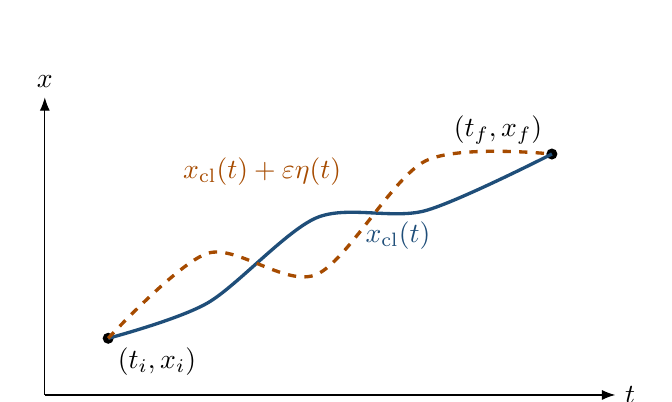
\begin{tikzpicture}[x=1.15cm,y=0.9cm,>=Latex]
    \draw[->] (0,0)--(6.3,0) node[right] {$t$};
    \draw[->] (0,0)--(0,4.2) node[above] {$x$};
    \coordinate (A) at (0.7,0.8);
    \coordinate (B) at (5.6,3.4);
    \fill (A) circle (2pt) node[below right] {$(t_i,x_i)$};
    \fill (B) circle (2pt) node[above left] {$(t_f,x_f)$};
    \draw[noteBlue,very thick]
      plot[smooth] coordinates {(0.7,0.8) (1.8,1.3) (3.0,2.5) (4.2,2.6) (5.6,3.4)};
    \draw[verifyOrange,very thick,dashed]
      plot[smooth] coordinates {(0.7,0.8) (1.8,2.0) (3.0,1.7) (4.2,3.3) (5.6,3.4)};
    \node[noteBlue] at (3.9,2.25) {$x_{\mathrm{cl}}(t)$};
    \node[verifyOrange] at (2.4,3.15) {$x_{\mathrm{cl}}(t)+\varepsilon\eta(t)$};
  \end{tikzpicture}
  \caption{固定同一对端点的经典路径与一条允许的邻近路径。}
  \label{fig:QM-C02-S01-path-variation}
\end{figure}

经典路径 $x_{\mathrm{cl}}(t)$ 满足 stationary-action condition（平稳作用量条件）
\begin{equation}
  \boxed{\delta S[x_{\mathrm{cl}}]=0.}
  \label{eq:QM-C02-S01-stationary-action}
\end{equation}
它表示任意允许的无穷小路径变形都不产生作用量的一阶变化，而不保证作用量一定是全局最小值。传统名称 principle of least action（最小作用量原理）因此不如 principle of stationary action（平稳作用量原理）准确。

自由粒子给出一个确实取到最小值的检验。令 $V=0$，连接固定端点的匀速路径为
\[
  x_{\mathrm{cl}}(t)
  =x_i+\frac{x_f-x_i}{t_f-t_i}(t-t_i).
\]
对任意满足 $\eta(t_i)=\eta(t_f)=0$ 的邻近路径 $x=x_{\mathrm{cl}}+\eta$，有
\begin{align}
  S[x]-S[x_{\mathrm{cl}}]
  &=m\int_{t_i}^{t_f}\dot x_{\mathrm{cl}}\dot\eta\,dt
    +\frac m2\int_{t_i}^{t_f}\dot\eta^2\,dt \notag\\
  &=m\dot x_{\mathrm{cl}}[\eta(t_f)-\eta(t_i)]
    +\frac m2\int_{t_i}^{t_f}\dot\eta^2\,dt \notag\\
  &=\frac m2\int_{t_i}^{t_f}\dot\eta^2\,dt\geq0.
  \label{eq:QM-C02-S01-free-particle-minimum}
\end{align}
这个例子中的匀速直线是最小作用量路径；一般问题只能由一阶变分推出平稳性。

\notetopic{QM-C02-S01-T02}{Euler--Lagrange 方程的完整变分推导}

在固定端点的经典路径附近构造一族路径
\begin{equation}
  x_\varepsilon(t)=x_{\mathrm{cl}}(t)+\varepsilon\eta(t),
  \qquad
  \eta(t_i)=\eta(t_f)=0.
  \label{eq:QM-C02-S01-varied-path}
\end{equation}
于是
\[
  \dot x_\varepsilon(t)
  =\dot x_{\mathrm{cl}}(t)+\varepsilon\dot\eta(t).
\]
把泛函限制在这族路径上，$S[x_\varepsilon]$ 成为普通参数 $\varepsilon$ 的函数。平稳条件为
\begin{equation}
  \left.\frac{d}{d\varepsilon}S[x_\varepsilon]
  \right|_{\varepsilon=0}=0.
  \label{eq:QM-C02-S01-epsilon-stationary}
\end{equation}
对式~\eqref{eq:QM-C02-S01-action} 使用链式法则，得到一阶变分
\begin{align}
  \delta S
  &=\left.\frac{d}{d\varepsilon}
    \int_{t_i}^{t_f}
    \mathcal L(x_\varepsilon,\dot x_\varepsilon,t)\,dt
    \right|_{\varepsilon=0} \notag\\
  &=\int_{t_i}^{t_f}
    \left(
      \frac{\partial\mathcal L}{\partial x}\eta
      +\frac{\partial\mathcal L}{\partial\dot x}\dot\eta
    \right)dt.
  \label{eq:QM-C02-S01-first-variation}
\end{align}
第二项含 $\dot\eta$，对其分部积分：
\begin{align}
  \int_{t_i}^{t_f}
  \frac{\partial\mathcal L}{\partial\dot x}\dot\eta\,dt
  &=\left[
    \frac{\partial\mathcal L}{\partial\dot x}\eta
    \right]_{t_i}^{t_f}
  -\int_{t_i}^{t_f}
    \frac{d}{dt}
    \left(\frac{\partial\mathcal L}{\partial\dot x}\right)
    \eta\,dt.
  \label{eq:QM-C02-S01-variation-integration-by-parts}
\end{align}
固定端点使边界项严格为零，故
\begin{equation}
  \delta S
  =\int_{t_i}^{t_f}
  \left[
    \frac{\partial\mathcal L}{\partial x}
    -\frac{d}{dt}
    \left(\frac{\partial\mathcal L}{\partial\dot x}\right)
  \right]\eta(t)\,dt.
  \label{eq:QM-C02-S01-variation-after-parts}
\end{equation}
若上式对所有内部任意、端点为零的 $\eta(t)$ 都等于零，则变分法基本引理要求方括号内逐点为零。否则若该函数在某个小邻域内同号，可选择只支撑在该邻域且同号的 $\eta$，使积分不为零。由此得到 Euler--Lagrange equation：
\begin{equation}
  \boxed{
  \frac{d}{dt}
  \left(\frac{\partial\mathcal L}{\partial\dot x}\right)
  -\frac{\partial\mathcal L}{\partial x}=0.}
  \label{eq:QM-C02-S01-euler-lagrange}
\end{equation}
逻辑上必须要求 $\delta S=0$ 对所有允许变分成立；单独某个 $\eta$ 使积分为零，可能只是正负贡献抵消，不能推出被积函数为零。

对 $n$ 个独立坐标，逐个变分可得
\begin{equation}
  \boxed{
  \frac{d}{dt}
  \left(\frac{\partial\mathcal L}{\partial\dot q_i}\right)
  -\frac{\partial\mathcal L}{\partial q_i}=0,
  \qquad i=1,\ldots,n.}
  \label{eq:QM-C02-S01-multicoordinate-euler-lagrange}
\end{equation}
推导只使用独立坐标、链式法则、分部积分和固定端点条件，并未要求 $q_i$ 是 Cartesian coordinates。

把式~\eqref{eq:QM-C02-S01-lagrangian} 代入式~\eqref{eq:QM-C02-S01-euler-lagrange}，有
\[
  \frac{\partial\mathcal L}{\partial\dot x}=m\dot x,
  \qquad
  \frac{\partial\mathcal L}{\partial x}=-\frac{dV}{dx},
\]
所以
\[
  m\ddot x=-\frac{dV}{dx},
\]
恢复 Newton 第二定律。简谐振子的直接应用见\relatedexercise{QM-C02-S01-E01}{教材练习 2.1.1}。

\notetopic{QM-C02-S01-T03}{广义坐标、正则动量与循环坐标}

能够无冗余地描述系统位形的独立参数 $q_i$ 称为 generalized coordinates（广义坐标）。它们可以是长度、角度或其他受约束系统的自然参数。由于式~\eqref{eq:QM-C02-S01-multicoordinate-euler-lagrange} 在任意这类坐标中形式不变，实际计算时可以选择最能反映几何约束和对称性的坐标。

定义与 $q_i$ 共轭的 canonical momentum（正则动量）
\begin{equation}
  \boxed{p_i=\frac{\partial\mathcal L}{\partial\dot q_i}}
  \label{eq:QM-C02-S01-canonical-momentum}
\end{equation}
后，Euler--Lagrange 方程可简写为
\begin{equation}
  \dot p_i=\frac{\partial\mathcal L}{\partial q_i}.
  \label{eq:QM-C02-S01-generalized-newton}
\end{equation}
右侧一般不能直接解释为物理力。标准的 generalized applied force（广义作用力）$Q_i^{\mathrm{appl}}$ 满足
\begin{equation}
  \boxed{
  \frac{d}{dt}\left(\frac{\partial T}{\partial\dot q_i}\right)
  -\frac{\partial T}{\partial q_i}
  =Q_i^{\mathrm{appl}}.}
  \label{eq:QM-C02-S01-generalized-force}
\end{equation}
若作用力来自速度无关的普通势能，则 $Q_i^{\mathrm{appl}}=-\partial V/\partial q_i$，式~\eqref{eq:QM-C02-S01-generalized-force} 与 $\mathcal L=T-V$ 的 Euler--Lagrange 方程等价。在这一保守势情形下有
\[
  \frac{\partial\mathcal L}{\partial q_i}
  =\frac{\partial T}{\partial q_i}+Q_i^{\mathrm{appl}},
\]
所以 $\partial\mathcal L/\partial q_i$ 还可能包含曲线坐标在动能中产生的几何项。只有在 Cartesian coordinates 且 $T$ 不显含位置时，它才直接退化为相应的物理力分量。$p_i$ 也不一定是 $m\dot q_i$；例如若 $q_i$ 是角度，对应的 $p_i$ 可为角动量。正则动量必须由式~\eqref{eq:QM-C02-S01-canonical-momentum} 计算，不能从名称猜测。

若完整 Lagrangian 不显含某个坐标 $q_j$，即
\begin{equation}
  \frac{\partial\mathcal L}{\partial q_j}=0,
  \label{eq:QM-C02-S01-cyclic-condition}
\end{equation}
则 $q_j$ 称为 cyclic coordinate（循环坐标），并有
\begin{equation}
  \boxed{p_j=\text{constant}.}
  \label{eq:QM-C02-S01-cyclic-conservation}
\end{equation}
判断时必须检查完整的 $\mathcal L$，不能只检查势能。坐标可以不出现在 $\mathcal L$ 中，而其速度 $\dot q_j$ 仍然出现；这正是相应正则动量非零且守恒的典型情形。

\notetopic{QM-C02-S01-T04}{教材例题 2.1.1：平面极坐标}

令
\[
  x=\rho\cos\phi,
  \qquad
  y=\rho\sin\phi.
\]
微分后平方相加：
\begin{align}
  dx&=\cos\phi\,d\rho-\rho\sin\phi\,d\phi,\notag\\
  dy&=\sin\phi\,d\rho+\rho\cos\phi\,d\phi,\notag\\
  ds^2=dx^2+dy^2&=d\rho^2+\rho^2d\phi^2.
  \label{eq:QM-C02-S01-polar-line-element}
\end{align}
因此速度平方和 Lagrangian 为
\begin{equation}
  v^2=\dot\rho^2+\rho^2\dot\phi^2,
  \qquad
  \mathcal L
  =\frac12m(\dot\rho^2+\rho^2\dot\phi^2)-V(\rho,\phi).
  \label{eq:QM-C02-S01-polar-lagrangian}
\end{equation}

\begin{figure}[htbp]
  \centering
  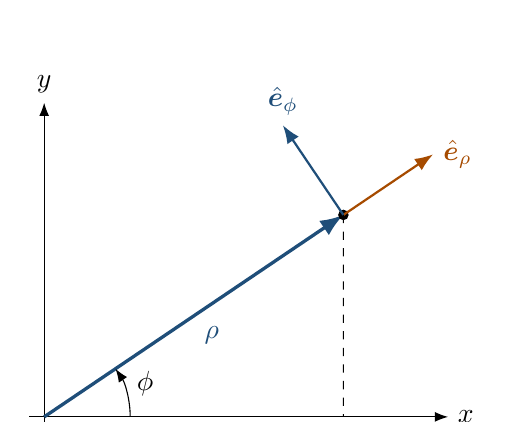
\begin{tikzpicture}[scale=0.95,>=Latex]
    \draw[->] (-0.2,0)--(5.4,0) node[right] {$x$};
    \draw[->] (0,-0.2)--(0,4.2) node[above] {$y$};
    \coordinate (P) at (4,2.7);
    \draw[noteBlue,very thick,->] (0,0)--(P) node[midway,below right] {$\rho$};
    \draw[->] (1.15,0) arc[start angle=0,end angle=34,radius=1.15];
    \node at (1.35,0.45) {$\phi$};
    \fill (P) circle (2pt);
    \draw[->,verifyOrange,thick] (P)--($(P)+(1.2,0.81)$) node[right] {$\hat{\bm e}_\rho$};
    \draw[->,noteBlue,thick] (P)--($(P)+(-0.81,1.2)$) node[above] {$\hat{\bm e}_\phi$};
    \draw[dashed] (P)--(4,0);
  \end{tikzpicture}
  \caption{极坐标的径向与角向基矢；基矢随 $\phi$ 改变。}
  \label{fig:QM-C02-S01-polar-basis}
\end{figure}

径向坐标给出
\begin{align}
  \frac{\partial\mathcal L}{\partial\dot\rho}&=m\dot\rho,
  &
  \frac{\partial\mathcal L}{\partial\rho}
  &=m\rho\dot\phi^2-\frac{\partial V}{\partial\rho},
\end{align}
故
\begin{equation}
  \boxed{
  m(\ddot\rho-\rho\dot\phi^2)
  =-\frac{\partial V}{\partial\rho}.}
  \label{eq:QM-C02-S01-polar-radial}
\end{equation}
角坐标给出
\begin{equation}
  \boxed{
  \frac{d}{dt}(m\rho^2\dot\phi)
  =-\frac{\partial V}{\partial\phi},}
  \label{eq:QM-C02-S01-polar-angular-conservative}
\end{equation}
或展开为
\begin{equation}
  \boxed{
  m(\rho\ddot\phi+2\dot\rho\dot\phi)
  =-\frac1\rho\frac{\partial V}{\partial\phi}.}
  \label{eq:QM-C02-S01-polar-angular}
\end{equation}
$-\rho\dot\phi^2$ 和 $2\dot\rho\dot\phi$ 来自曲线坐标基的变化；Lagrange 方法把这些几何信息编码在动能中，无须单独对旋转基矢求导。
特别地，$\partial\mathcal L/\partial\rho=m\rho\dot\phi^2-\partial V/\partial\rho$ 中，$m\rho\dot\phi^2$ 是动能的坐标导数，不是额外的径向作用力。真正的径向物理力为 $-\partial V/\partial\rho$，而完整径向加速度是 $\ddot\rho-\rho\dot\phi^2$。

若 $V=V(\rho)$，则 $\phi$ 是循环坐标，
\begin{equation}
  p_\phi=m\rho^2\dot\phi=L_z=\text{constant}.
  \label{eq:QM-C02-S01-polar-angular-momentum}
\end{equation}
相应的面积速度为
\begin{equation}
  \frac{dA}{dt}=\frac12\rho^2\dot\phi=\frac{L_z}{2m},
  \label{eq:QM-C02-S01-areal-velocity}
\end{equation}
所以中心力运动满足等时扫过等面积。教材例题还表明，适当选取坐标后，守恒量常可由“某坐标不显含于 $\mathcal L$”直接读出。

\notetopic{QM-C02-S01-T05}{三维中心势中的球坐标与角动量}

球坐标的线元为
\begin{equation}
  ds^2=dr^2+r^2d\theta^2+r^2\sin^2\theta\,d\phi^2.
  \label{eq:QM-C02-S01-spherical-line-element}
\end{equation}
对中心势 $V(r)$，
\begin{equation}
  \mathcal L
  =\frac12m\left(
    \dot r^2+r^2\dot\theta^2
    +r^2\sin^2\theta\,\dot\phi^2
  \right)-V(r).
  \label{eq:QM-C02-S01-spherical-lagrangian}
\end{equation}
虽然 $V$ 与 $\theta$ 无关，但动能显含 $\sin^2\theta$，所以 $\theta$ 不是循环坐标。$\phi$ 不显含于完整的 $\mathcal L$，因此
\begin{equation}
  p_\phi=mr^2\sin^2\theta\,\dot\phi=L_z
  \label{eq:QM-C02-S01-spherical-p-phi}
\end{equation}
守恒。球坐标选定的 $z$ 轴使绕该轴的旋转表现为 $\phi\mapsto\phi+\alpha$，所以 $L_z$ 的守恒最直接；中心势的完整旋转对称性实际上还保证整个角动量向量守恒：
\begin{equation}
  \frac{d\bm L}{dt}=\bm r\times\bm F=0,
  \qquad
  L^2=p_\theta^2+\frac{p_\phi^2}{\sin^2\theta}.
  \label{eq:QM-C02-S01-full-angular-momentum}
\end{equation}
球坐标下的三条运动方程及循环坐标判断见\relatedexercise{QM-C02-S01-E03}{教材练习 2.1.3}。

\subsection{适用条件与常见误区}

\begin{itemize}[leftmargin=*]
  \item $\delta S=0$ 只说明一阶变分为零，不自动说明作用量取得全局最小值。
  \item 固定端点条件用于消去分部积分产生的边界项；若端点允许变化，还会出现额外的自然边界条件。
  \item $\mathcal L=T-V$ 适用于本节的速度无关保守势。后续电磁相互作用表明，一般 Lagrangian 不必具有这一形式。
  \item 正则动量由 $p_i=\partial\mathcal L/\partial\dot q_i$ 定义，不一定等于机械动量 $m\dot q_i$。
  \item 判断循环坐标必须检查完整的 $\mathcal L$，不能只检查 $V$。
\end{itemize}

\subsection{一分钟回顾}

作用量是以整条路径为输入的泛函，经典路径使其一阶变分为零。固定端点和分部积分把平稳条件转化为 Euler--Lagrange 方程，其形式对任意合适的广义坐标保持不变。正则动量是 Lagrangian 对广义速度的偏导；若某坐标不显含于完整 Lagrangian，对应正则动量守恒。极坐标例题展示了曲线坐标的几何项如何由动能自动产生，也把旋转对称性与角动量守恒联系起来。

\section{第 2.2 节：电磁场中的 Lagrangian}
\label{section:QM-C02-S02}

\studymeta
  {QM-C02-S02}
  {2026-08-28}
  {Shankar, \textit{Principles of Quantum Mechanics}, Second Edition}
  {第 2 章 \S 2.2；印刷页 pp.~83--84；PDF pp.~96--97}
  {正文已核对；本节无教材例题或习题，配套题明确标为自编检验题}

\subsection{本节主线}

普通位置势 $V(\bm r,t)$ 只能产生梯度力，无法表示显式依赖速度的磁力。本节把 scalar potential（标势）$\phi$ 与 vector potential（矢势）$\bm A$ 写入 Lagrangian，并由 Euler--Lagrange 方程恢复完整 Lorentz force（洛伦兹力）。这一过程还迫使我们区分 canonical momentum（正则动量）与 mechanical momentum（机械动量），也说明“外力”“约束力”与“是否写在 Euler--Lagrange 方程右侧”不是同一分类标准。

\notetopic{QM-C02-S02-T01}{普通位置势的不足与电磁 Lagrangian}

教材使用 Gaussian units（高斯单位制），其中 Lorentz force 为
\begin{equation}
  \boxed{
  \bm F=q\left(\bm E+\frac{\bm v}{c}\times\bm B\right).}
  \label{eq:QM-C02-S02-lorentz-force}
\end{equation}
若 $\mathcal L=\frac12m\bm v^2-V(\bm r,t)$，则 Euler--Lagrange 方程只能给出 $m\dot{\bm v}=-\nabla V$，无法产生速度依赖项 $q\bm v\times\bm B/c$。正确的电磁 Lagrangian 是
\begin{equation}
  \boxed{
  \mathcal L_{\mathrm{em}}
  =\frac12m\bm v^2-q\phi(\bm r,t)
  +\frac qc\bm v\cdot\bm A(\bm r,t).}
  \label{eq:QM-C02-S02-em-lagrangian}
\end{equation}
$\bm v\cdot\bm A$ 是旋转下的标量；它对速度求偏导留下 $\bm A$，对位置求偏导产生 $\bm A$ 的空间导数，二者在 Euler--Lagrange 方程中组合成 $\nabla\times\bm A$。在 SI units 中，式~\eqref{eq:QM-C02-S02-lorentz-force} 和式~\eqref{eq:QM-C02-S02-em-lagrangian} 中相应的 $1/c$ 均不出现。

\notetopic{QM-C02-S02-T02}{标势、矢势与规范自由度}

势的表示不是从 Lagrangian 中倒推定义出来的，而是源于 homogeneous Maxwell equations（齐次 Maxwell 方程）
\begin{equation}
  \nabla\cdot\bm B=0,
  \qquad
  \nabla\times\bm E=-\frac1c\frac{\partial\bm B}{\partial t}.
  \label{eq:QM-C02-S02-homogeneous-maxwell}
\end{equation}
在拓扑足够简单的区域内，散度为零的光滑向量场可局部写成另一个向量场的旋度，因此
\begin{equation}
  \boxed{\bm B=\nabla\times\bm A.}
  \label{eq:QM-C02-S02-vector-potential}
\end{equation}
根据 Stokes theorem，$\oint_{\partial S}\bm A\cdot d\bm l=\int_S\bm B\cdot d\bm S$，所以 $\bm A$ 沿闭合曲线的环流编码了曲线内部的磁通量。
\begin{figure}[htbp]
  \centering
  \begin{tikzpicture}[scale=0.9,>=Latex]
    \fill[noteBlue!8] (0,0) ellipse (3.0 and 1.35);
    \draw[noteBlue,very thick] (0,0) ellipse (3.0 and 1.35);
    \draw[->,noteBlue,very thick]
      (2.82,-0.45) arc[start angle=-20,end angle=32,x radius=3.0,y radius=1.35];
    \node[noteBlue] at (3.55,0.55) {$C=\partial S$};
    \node at (-2.35,-0.8) {$S$};
    \foreach \x/\y in {-1.8/0.35,-0.9/-0.45,0/0.45,0.9/-0.35,1.8/0.3}
      {\node[verifyOrange] at (\x,\y) {$\odot$};}
    \node[verifyOrange] at (0,-1.85) {$\bm B$ 穿过曲面};
  \end{tikzpicture}
  \caption{Stokes theorem 把边界上的矢势环流与穿过曲面的磁通量联系起来；箭头只表示闭合曲线的正向。}
  \label{fig:QM-C02-S02-stokes}
\end{figure}
把式~\eqref{eq:QM-C02-S02-vector-potential} 代入 Faraday's law，有
\[
  \nabla\times\left(
    \bm E+\frac1c\frac{\partial\bm A}{\partial t}
  \right)=0.
\]
无旋场可局部写成标量势的负梯度，故
\begin{equation}
  \boxed{
  \bm E=-\nabla\phi-\frac1c\frac{\partial\bm A}{\partial t}.}
  \label{eq:QM-C02-S02-scalar-potential}
\end{equation}
当磁场随时间变化时，$\nabla\times\bm E$ 一般非零，因而不能只写 $\bm E=-\nabla\phi$。

势并不唯一。对任意足够光滑的 $\chi(\bm r,t)$，gauge transformation（规范变换）
\begin{equation}
  \bm A'=\bm A+\nabla\chi,
  \qquad
  \phi'=\phi-\frac1c\frac{\partial\chi}{\partial t}
  \label{eq:QM-C02-S02-gauge-transform}
\end{equation}
保持 $\bm E$ 与 $\bm B$ 不变，同时令
\begin{equation}
  \mathcal L_{\mathrm{em}}'
  =\mathcal L_{\mathrm{em}}+\frac qc\frac{d\chi}{dt}.
  \label{eq:QM-C02-S02-gauge-lagrangian}
\end{equation}
作用量只增加固定端点处的边界值 $\frac qc[\chi_f-\chi_i]$，所以 Euler--Lagrange 方程不变。这把规范自由度与第 2.1 节的固定端点变分直接联系起来。若空间区域具有非平凡拓扑，全局单一光滑矢势可能不存在；本节只需使用上述局部关系。

\notetopic{QM-C02-S02-T03}{从 Lagrangian 完整恢复 Lorentz force}

令 $x_i$ 为 Cartesian coordinates、$v_i=\dot x_i$，并把式~\eqref{eq:QM-C02-S02-em-lagrangian} 写成
\[
  \mathcal L_{\mathrm{em}}
  =\frac12m\sum_jv_j^2-q\phi
  +\frac qc\sum_jv_jA_j.
\]
首先
\begin{equation}
  \frac{\partial\mathcal L_{\mathrm{em}}}{\partial v_i}
  =mv_i+\frac qcA_i.
  \label{eq:QM-C02-S02-dl-dv}
\end{equation}
由于 $A_i=A_i(\bm r(t),t)$，沿粒子轨迹的全导数必须同时包含显式时间变化与位置变化：
\begin{equation}
  \frac{dA_i}{dt}
  =\frac{\partial A_i}{\partial t}
  +\sum_jv_j\frac{\partial A_i}{\partial x_j}.
  \label{eq:QM-C02-S02-total-derivative-A}
\end{equation}
因此
\begin{equation}
  \frac{d}{dt}
  \left(\frac{\partial\mathcal L_{\mathrm{em}}}{\partial v_i}\right)
  =m\dot v_i+\frac qc\frac{\partial A_i}{\partial t}
  +\frac qc\sum_jv_j\frac{\partial A_i}{\partial x_j}.
  \label{eq:QM-C02-S02-dt-dl-dv}
\end{equation}
另一方面，求 $\partial/\partial x_i$ 时各 $v_j$ 作为独立变量保持不变，故
\begin{equation}
  \frac{\partial\mathcal L_{\mathrm{em}}}{\partial x_i}
  =-q\frac{\partial\phi}{\partial x_i}
  +\frac qc\sum_jv_j\frac{\partial A_j}{\partial x_i}.
  \label{eq:QM-C02-S02-dl-dx}
\end{equation}
代入 Euler--Lagrange 方程并整理：
\begin{align}
  m\dot v_i
  &=-q\frac{\partial\phi}{\partial x_i}
    -\frac qc\frac{\partial A_i}{\partial t}
    +\frac qc\sum_jv_j
      \left(
        \frac{\partial A_j}{\partial x_i}
        -\frac{\partial A_i}{\partial x_j}
      \right)\notag\\
  &=qE_i+\frac qc(\bm v\times\bm B)_i.
  \label{eq:QM-C02-S02-lorentz-components}
\end{align}
最后一步使用
\begin{equation}
  [\bm v\times(\nabla\times\bm A)]_i
  =\sum_jv_j
  \left(
    \frac{\partial A_j}{\partial x_i}
    -\frac{\partial A_i}{\partial x_j}
  \right).
  \label{eq:QM-C02-S02-curl-identity}
\end{equation}
三个分量合并后正好恢复式~\eqref{eq:QM-C02-S02-lorentz-force}。推导中最容易遗漏的是式~\eqref{eq:QM-C02-S02-total-derivative-A} 的对流项 $\sum_jv_j\partial A_i/\partial x_j$；没有它就无法形成 curl 的反对称导数组合。

\notetopic{QM-C02-S02-T04}{正则动量、机械动量与广义势}

由式~\eqref{eq:QM-C02-S02-dl-dv}，canonical momentum 为
\begin{equation}
  \boxed{
  \bm p=\frac{\partial\mathcal L_{\mathrm{em}}}{\partial\bm v}
  =m\bm v+\frac qc\bm A.}
  \label{eq:QM-C02-S02-canonical-momentum}
\end{equation}
mechanical momentum 记作 $\bm\pi=m\bm v$，所以
\begin{equation}
  \boxed{\bm\pi=\bm p-\frac qc\bm A.}
  \label{eq:QM-C02-S02-mechanical-momentum}
\end{equation}
规范变换会使 $\bm p'=\bm p+q\nabla\chi/c$，但式~\eqref{eq:QM-C02-S02-mechanical-momentum} 中的组合保持不变。正则动量是与坐标共轭的变量，机械动量则直接由速度决定；在电磁场中不能把符号 $\bm p$ 自动替换成 $m\bm v$。

形式上可定义 velocity-dependent generalized potential（速度依赖广义势）
\begin{equation}
  U(\bm r,\bm v,t)
  =q\phi-\frac qc\bm v\cdot\bm A,
  \qquad
  \mathcal L_{\mathrm{em}}=T-U.
  \label{eq:QM-C02-S02-generalized-potential}
\end{equation}
对于这类 $U$，物理广义力不再是 $-\partial U/\partial q_i$，而是
\begin{equation}
  \boxed{
  Q_i^{\mathrm{appl}}
  =\frac{d}{dt}\left(\frac{\partial U}{\partial\dot q_i}\right)
  -\frac{\partial U}{\partial q_i}.}
  \label{eq:QM-C02-S02-velocity-potential-force}
\end{equation}
磁力恒满足 $(q\bm v\times\bm B/c)\cdot\bm v=0$，会改变轨迹方向但不做功。因此 $-q\bm v\cdot\bm A/c$ 不能解释为普通磁势能；Lagrangian 本身也不是系统能量。

\notetopic{QM-C02-S02-T05}{相互作用、坐标几何、约束与非保守力}

Euler--Lagrange 方程右侧为零，不表示系统没有外力；它表示当前模型中由作用量描述的相互作用已经写入 $\mathcal L$。是否由外部给定，不是判断某个作用是否需要放在方程右侧的标准。例如给定电磁场虽可视为外场，其作用已经包含在式~\eqref{eq:QM-C02-S02-em-lagrangian} 中。

需要区分以下来源：
\begin{itemize}[leftmargin=*]
  \item \textbf{坐标几何：}曲线坐标使 $T$ 显含 $q_i$，产生的项用于组装该坐标系中的完整加速度，不是额外物理力。
  \item \textbf{速度依赖相互作用：}即使使用 Cartesian coordinates，$\bm v\cdot\bm A$ 仍会把正则动量从 $m\bm v$ 移开；这是相互作用本身造成的。
  \item \textbf{理想完整约束：}可用独立广义坐标消去约束，或用 Lagrange multiplier（拉格朗日乘子）保留并求出约束力。
  \item \textbf{未写入 $\mathcal L$ 的非保守作用：}使用 Lagrange--d'Alembert equation
  \begin{equation}
    \frac{d}{dt}\left(\frac{\partial\mathcal L}{\partial\dot q_i}\right)
    -\frac{\partial\mathcal L}{\partial q_i}
    =Q_i^{\mathrm{nc}}.
    \label{eq:QM-C02-S02-lagrange-dalembert}
  \end{equation}
\end{itemize}
仅写 $V=0$ 不能推出没有物理力，还必须排除未建模的外加作用与约束力。反过来，非零角动量也不意味着存在力：不经过坐标原点的自由直线运动可以具有非零且守恒的角动量。固定长度绳子的建模见\relatedexercise{QM-C02-S02-E02}{自编检验题 2}。

\subsection{适用条件与常见误区}

\begin{itemize}[leftmargin=*]
  \item 教材本节使用 Gaussian units；与 SI 公式比较时必须同步处理 $1/c$。
  \item $dA_i/dt$ 是沿粒子轨迹的全导数，不能误写成 $\partial A_i/\partial t$。
  \item $\bm B=\nabla\times\bm A$ 与式~\eqref{eq:QM-C02-S02-scalar-potential} 来自齐次 Maxwell 方程，不是为匹配 Lorentz force 临时定义的。
  \item 正则动量依赖规范，机械动量及由 $\bm E,\bm B$ 决定的运动不依赖规范。
  \item $V=0$ 只排除了所写的普通势能，不能自动排除约束力、摩擦力或其他未建模作用。
\end{itemize}

\subsection{一分钟回顾}

齐次 Maxwell 方程允许用 $\phi$ 与 $\bm A$ 表示电磁场；电磁 Lagrangian 中的 $\bm v\cdot\bm A$ 项通过反对称空间导数组合产生磁力。正则动量为 $\bm p=m\bm v+q\bm A/c$，而可直接由速度确定的机械动量为 $m\bm v$。规范变换只让 Lagrangian 增加全时间导数，不改变场和运动。坐标几何、速度依赖相互作用、理想约束与未建模非保守力必须在建模时分别处理。

\section{第 2.3 节：二体问题}
\label{section:QM-C02-S03}

\studymeta
  {QM-C02-S03}
  {2026-08-29}
  {Shankar, \textit{Principles of Quantum Mechanics}, Second Edition}
  {第 2 章 \S 2.3；印刷页 pp.~85--86；PDF pp.~98--99}
  {正文及教材练习 2.3.1 已核对；坐标变换、约化质量与适用条件已补全}

\subsection{本节主线}

两个只通过内部势相互作用、且不受外力的粒子，表面上需要同时求解 $\bm r_1(t)$ 与 $\bm r_2(t)$。改用 center-of-mass coordinate（质心坐标）$\bm R$ 和 relative coordinate（相对坐标）$\bm r$ 后，Lagrangian 可以分成互不耦合的质心运动与相对运动。原二体问题由此化为两个单粒子问题：一个质量为总质量 $M$ 的自由质心粒子，以及一个质量为 reduced mass（约化质量）$\mu$、在势 $V(\bm r)$ 中运动的等效粒子。

\notetopic{QM-C02-S03-T01}{建模假设与质心--相对坐标}

设两粒子的质量和位置分别为 $m_1,m_2$ 与 $\bm r_1,\bm r_2$。本节假设没有外力，且内部势只依赖两粒子的相对位置：
\begin{equation}
  V=V(\bm r_1-\bm r_2).
  \label{eq:QM-C02-S03-relative-potential}
\end{equation}
定义总质量、相对坐标和质心坐标
\begin{equation}
  M=m_1+m_2,
  \qquad
  \bm r=\bm r_1-\bm r_2,
  \qquad
  \bm R=\frac{m_1\bm r_1+m_2\bm r_2}{M}.
  \label{eq:QM-C02-S03-coordinate-definitions}
\end{equation}
解这个线性方程组可得逆变换
\begin{equation}
  \boxed{
  \bm r_1=\bm R+\frac{m_2}{M}\bm r,
  \qquad
  \bm r_2=\bm R-\frac{m_1}{M}\bm r.}
  \label{eq:QM-C02-S03-inverse-transform}
\end{equation}
例如 $m_1=3m,m_2=m$ 时，$\bm r_1=\bm R+\bm r/4$、$\bm r_2=\bm R-3\bm r/4$；较重的粒子离质心较近。

若把整个系统平移同一向量 $\bm a$，则
\begin{equation}
  \bm r_1\mapsto\bm r_1+\bm a,
  \quad
  \bm r_2\mapsto\bm r_2+\bm a,
  \quad
  \bm R\mapsto\bm R+\bm a,
  \quad
  \bm r\mapsto\bm r.
  \label{eq:QM-C02-S03-translation}
\end{equation}
因此 $V(\bm r)$ 对整体平移不敏感。能够分离质心运动的关键不是“势能不含 $\dot{\bm r}$”，而是势能不含 $\bm R$；前者对普通位置势本来就成立，后者才表达系统的平移不变性。

\notetopic{QM-C02-S03-T02}{动能分离与约化质量}

原 Lagrangian 为
\begin{equation}
  \mathcal L
  =\frac12m_1|\dot{\bm r}_1|^2
  +\frac12m_2|\dot{\bm r}_2|^2
  -V(\bm r_1-\bm r_2).
  \label{eq:QM-C02-S03-original-lagrangian}
\end{equation}
对式~\eqref{eq:QM-C02-S03-inverse-transform} 求时间导数：
\begin{equation}
  \dot{\bm r}_1=\dot{\bm R}+\frac{m_2}{M}\dot{\bm r},
  \qquad
  \dot{\bm r}_2=\dot{\bm R}-\frac{m_1}{M}\dot{\bm r}.
  \label{eq:QM-C02-S03-velocity-transform}
\end{equation}
代入动能并展开，第一部分为
\begin{align}
  \frac12m_1|\dot{\bm r}_1|^2
  ={}&\frac12m_1|\dot{\bm R}|^2
  +\frac{m_1m_2}{M}\dot{\bm R}\cdot\dot{\bm r}
  +\frac12m_1\frac{m_2^2}{M^2}|\dot{\bm r}|^2,
  \label{eq:QM-C02-S03-first-kinetic-expansion}
\end{align}
第二部分为
\begin{align}
  \frac12m_2|\dot{\bm r}_2|^2
  ={}&\frac12m_2|\dot{\bm R}|^2
  -\frac{m_1m_2}{M}\dot{\bm R}\cdot\dot{\bm r}
  +\frac12m_2\frac{m_1^2}{M^2}|\dot{\bm r}|^2.
  \label{eq:QM-C02-S03-second-kinetic-expansion}
\end{align}
交叉项恰好抵消。相对速度平方项的系数满足
\begin{align}
  m_1\frac{m_2^2}{M^2}+m_2\frac{m_1^2}{M^2}
  &=\frac{m_1m_2(m_1+m_2)}{M^2}
   =\frac{m_1m_2}{m_1+m_2}.
  \label{eq:QM-C02-S03-reduced-mass-coefficient}
\end{align}
定义
\begin{equation}
  \boxed{
  \mu=\frac{m_1m_2}{m_1+m_2},
  \qquad
  \frac1\mu=\frac1{m_1}+\frac1{m_2}.}
  \label{eq:QM-C02-S03-reduced-mass}
\end{equation}
于是
\begin{equation}
  \boxed{
  \mathcal L
  =\frac12M|\dot{\bm R}|^2
  +\frac12\mu|\dot{\bm r}|^2
  -V(\bm r).}
  \label{eq:QM-C02-S03-separated-lagrangian}
\end{equation}
教材练习 2.3.1 要求完成这一变量代换，完整计算见\relatedexercise{QM-C02-S03-E01}{教材练习 2.3.1}。

\notetopic{QM-C02-S03-T03}{两个互不耦合的单粒子问题}

式~\eqref{eq:QM-C02-S03-separated-lagrangian} 可以写成
\begin{equation}
  \mathcal L
  =\underbrace{\frac12M|\dot{\bm R}|^2}_{\mathcal L_{\mathrm{CM}}}
  +\underbrace{\left(\frac12\mu|\dot{\bm r}|^2-V(\bm r)\right)}_{\mathcal L_{\mathrm{rel}}}.
  \label{eq:QM-C02-S03-lagrangian-parts}
\end{equation}
质心坐标不显含于 $\mathcal L$，所以它是循环坐标，其共轭动量为
\begin{equation}
  \boxed{
  \bm P=\frac{\partial\mathcal L}{\partial\dot{\bm R}}
  =M\dot{\bm R}
  =m_1\dot{\bm r}_1+m_2\dot{\bm r}_2,}
  \qquad
  \dot{\bm P}=0.
  \label{eq:QM-C02-S03-total-momentum}
\end{equation}
这正是系统总动量。相对坐标的共轭动量和两组运动方程为
\begin{equation}
  \boxed{
  \bm p=\mu\dot{\bm r},
  \qquad
  M\ddot{\bm R}=0,
  \qquad
  \mu\ddot{\bm r}=-\nabla_{\bm r}V(\bm r).}
  \label{eq:QM-C02-S03-equations-of-motion}
\end{equation}
因此第一个等效粒子质量为 $M$，做自由质心运动；第二个等效粒子质量为 $\mu$，在势 $V(\bm r)$ 中运动。它们只是对原坐标的等效描述，并不表示系统中真的新增了两个粒子。

在 center-of-mass frame（质心参考系）中取 $\bm R=0$、$\dot{\bm R}=0$，则
\begin{equation}
  \dot{\bm r}_1=\frac{m_2}{M}\dot{\bm r},
  \qquad
  \dot{\bm r}_2=-\frac{m_1}{M}\dot{\bm r},
  \label{eq:QM-C02-S03-cm-velocities}
\end{equation}
并且
\begin{equation}
  m_1\dot{\bm r}_1=\mu\dot{\bm r}=\bm p,
  \qquad
  m_2\dot{\bm r}_2=-\mu\dot{\bm r}=-\bm p.
  \label{eq:QM-C02-S03-cm-momenta}
\end{equation}
研究内部运动时可以忽略平凡的质心匀速运动，但这不表示质心运动不存在；只是在质心参考系中把它消去了。

\notetopic{QM-C02-S03-T04}{从 Newton 方程理解约化质量}

设粒子 1 受到的内部力为 $\bm F$，粒子 2 受到的内部力为 $-\bm F$。由
\begin{equation}
  m_1\ddot{\bm r}_1=\bm F,
  \qquad
  m_2\ddot{\bm r}_2=-\bm F
  \label{eq:QM-C02-S03-newton-pair}
\end{equation}
可得
\begin{align}
  \ddot{\bm r}
  &=\ddot{\bm r}_1-\ddot{\bm r}_2
    =\left(\frac1{m_1}+\frac1{m_2}\right)\bm F
    =\frac{\bm F}{\mu},
\end{align}
即
\begin{equation}
  \boxed{\mu\ddot{\bm r}=\bm F.}
  \label{eq:QM-C02-S03-newton-reduced-mass}
\end{equation}
若 $\bm F=-\nabla_{\bm r}V$，这正是式~\eqref{eq:QM-C02-S03-equations-of-motion} 的相对运动方程。约化质量把两个物体共同改变相对距离的效果压缩进一个等效惯性参数中。因为
\[
  \frac1\mu=\frac1{m_1}+\frac1{m_2},
\]
所以 $\mu<\min(m_1,m_2)$。两个常用极限是
\begin{equation}
  m_2\gg m_1\Longrightarrow\mu\simeq m_1,
  \qquad
  m_1=m_2=m\Longrightarrow\mu=\frac m2.
  \label{eq:QM-C02-S03-reduced-mass-limits}
\end{equation}
第一种情形表示重粒子近似固定，轻粒子近似以自身质量在势中运动；第二种情形中两粒子的加速度大小相等、方向相反，因此相对加速度是任一粒子加速度的两倍。$\mu=m/2$ 仍只是相对运动的等效质量，不是新的真实粒子。

\notetopic{QM-C02-S03-T05}{分离成立的条件}

坐标变换式~\eqref{eq:QM-C02-S03-coordinate-definitions} 总可以进行，但动力学分离还依赖模型结构：
\begin{itemize}[leftmargin=*]
  \item 内部相互作用只依赖 $\bm r_1-\bm r_2$，因而不显含 $\bm R$；
  \item 系统没有把 $\bm R$ 与 $\bm r$ 重新耦合的一般外势；
  \item 质心与相对坐标的动能交叉项因质量加权的质心定义而抵消。
\end{itemize}
例如，只作用于粒子 1 的外势会变为
\begin{equation}
  U(\bm r_1)
  =U\left(\bm R+\frac{m_2}{M}\bm r\right),
  \label{eq:QM-C02-S03-external-potential}
\end{equation}
一般同时依赖 $\bm R$ 与 $\bm r$，从而破坏分离。这里必须保留“一般”二字：特殊外势仍可能分解成纯质心项与纯相对项。另外，二体分离只要求 $V=V(\bm r)$；更强的 central potential 条件 $V=V(|\bm r|)$ 还会进一步带来相对运动的旋转对称性和角动量守恒。

\subsection{适用条件与常见误区}

\begin{itemize}[leftmargin=*]
  \item 约化质量是相对坐标的等效惯性参数，不是任何一个真实粒子的质量。
  \item $M\ddot{\bm R}=0$ 表示质心做匀速运动，不表示质心坐标可以在所有参考系中直接删除。
  \item 势能不含 $\dot{\bm r}$ 不是分离的理由；关键是 $V$ 不含 $\bm R$。
  \item 改变量本身不减少自由度，而是把原先耦合的自由度改写成更合适的独立组合。
  \item 一般外势会耦合 $\bm R$ 与 $\bm r$；是否仍能分离必须代入具体势后判断。
\end{itemize}

\subsection{一分钟回顾}

质量加权的质心坐标与相对坐标把二体 Lagrangian 对角化为质心部分和相对部分。质心以总质量 $M$ 做自由匀速运动，总动量守恒；相对坐标则等价于一个质量为 $\mu=m_1m_2/(m_1+m_2)$ 的粒子在势 $V(\bm r)$ 中运动。约化质量既可从动能展开得到，也可从两条 Newton 方程相减得到。真正保证分离的是平移不变的内部势与无一般外势，而不是简单地把二体问题“少算一个粒子”。

\section{第 2.4 节：粒子有多聪明？}
\label{section:QM-C02-S04}

\studymeta
  {QM-C02-S04}
  {2026-08-30}
  {Shankar, \textit{Principles of Quantum Mechanics}, Second Edition}
  {第 2 章 \S 2.4；印刷页 p.~86；PDF p.~99}
  {正文已核对；本节无教材例题或习题，配套题明确标为自编检验题}

\subsection{本节主线}

作用量以整条路径为输入，固定起点与终点后再要求 $\delta S=0$，形式上似乎暗示粒子必须预先知道终点、比较所有路径后才选择运动方式。本节指出这种 teleological（目的论式）理解是错觉：全局的变分表述会导出局部 Euler--Lagrange 方程，经典粒子只需服从当前时刻的局部运动规律。教材随后预告 path integral（路径积分）：量子传播对所有路径的复振幅求和，而经典路径在适当极限中由 stationary phase（平稳相位）机制显现。

\notetopic{QM-C02-S04-T01}{全局变分不等于粒子预知未来}

对固定端点 $x(t_i)=x_i$、$x(t_f)=x_f$，作用量为
\begin{equation}
  S[x]=\int_{t_i}^{t_f}
  \mathcal L(x,\dot x,t)\,dt.
  \label{eq:QM-C02-S04-action}
\end{equation}
允许变分满足
\[
  x(t)\mapsto x(t)+\epsilon\eta(t),
  \qquad
  \eta(t_i)=\eta(t_f)=0.
\]
第 2.1 节的推导给出
\begin{equation}
  \delta S
  =\int_{t_i}^{t_f}
  \left[
    \frac{\partial\mathcal L}{\partial x}
    -\frac{d}{dt}
      \left(\frac{\partial\mathcal L}{\partial\dot x}\right)
  \right]\eta(t)\,dt.
  \label{eq:QM-C02-S04-first-variation}
\end{equation}
由于该式对所有允许的 $\eta(t)$ 都为零，得到局部方程
\begin{equation}
  \boxed{
  \frac{d}{dt}
  \left(\frac{\partial\mathcal L}{\partial\dot x}\right)
  -\frac{\partial\mathcal L}{\partial x}=0.}
  \label{eq:QM-C02-S04-euler-lagrange}
\end{equation}
因此，“对整条路径取变分”是描述运动规律的数学形式，不表示粒子在物理上逐条计算候选路径。

需要区分两种求解方式：
\begin{itemize}[leftmargin=*]
  \item \textbf{Initial-value problem（初值问题）：}给定 $x(t_i)$ 与 $\dot x(t_i)$，用局部微分方程向未来演化；
  \item \textbf{Boundary-value problem（边值问题）：}给定 $x(t_i)$ 与 $x(t_f)$，寻找满足这些边界条件的平稳路径。
\end{itemize}
未来终点是求解者对边值问题施加的条件，用于从可能的运动中选出符合边界的轨迹；它不是粒子获得的未来信息。对
\begin{equation}
  \mathcal L=\frac12m\dot x^2-V(x,t)
  \label{eq:QM-C02-S04-standard-lagrangian}
\end{equation}
有
\begin{equation}
  \boxed{
  m\ddot x=-\frac{\partial V(x,t)}{\partial x}.}
  \label{eq:QM-C02-S04-local-newton}
\end{equation}
当前加速度只由当前的 $x,t$ 和该处势能梯度决定；在更一般的速度依赖 Lagrangian 中，局部运动还可能依赖当前速度。

\notetopic{QM-C02-S04-T02}{Stationary 不等于 minimum}

教材沿用 principle of least action（最小作用量原理）的传统名称，并在本节使用“选择最小作用量路径”的直观措辞。严格条件仍然是
\begin{equation}
  \boxed{\delta S=0,}
  \label{eq:QM-C02-S04-stationary-action}
\end{equation}
即作用量在经典路径处 stationary（平稳）。它可能是局部最小值、局部最大值或 saddle point（鞍点）；仅有一阶变分为零不能判断二阶性质。因此本节的 least/minimize 应理解为传统而宽松的表述。

教材还说粒子只需探测附近的势并沿变化最快的方向加速。对 Cartesian coordinates 下的普通保守系统
\[
  \mathcal L=\frac12m|\dot{\bm r}|^2-V(\bm r,t)
\]
确有 $m\ddot{\bm r}=-\nabla V$。但电磁场、曲线坐标、约束或速度依赖相互作用中的局部 Euler--Lagrange 方程不一定能简化为这一形式。

\notetopic{QM-C02-S04-T03}{路径积分预告与经典路径的显现}

本节只作概念预告；后续 Feynman path integral 的标准形式为
\begin{equation}
  K(x_f,t_f;x_i,t_i)
  =\int\mathcal D x(t)\,
  \exp\left(\frac{i}{\hbar}S[x]\right).
  \label{eq:QM-C02-S04-path-integral}
\end{equation}
$K$ 是从初始时空点传播到末时空点的 quantum amplitude（量子振幅），$\int\mathcal D x(t)$ 形式上表示对所有连接端点的路径求和。对普通实作用量，单条路径的因子满足
\begin{equation}
  \left|
    \exp\left(\frac{i}{\hbar}S[x]\right)
  \right|=1,
  \label{eq:QM-C02-S04-equal-modulus}
\end{equation}
所以教材所说的 equal weight 应理解为相同模长的复振幅，而不是各路径具有相同经典概率；不同路径的相位 $S[x]/\hbar$ 仍然不同。

在经典路径 $x_{\mathrm{cl}}$ 附近令 $x=x_{\mathrm{cl}}+\eta$，有泛函 Taylor 展开
\begin{equation}
  S[x_{\mathrm{cl}}+\eta]
  =S[x_{\mathrm{cl}}]
  +\delta S
  +\frac12\delta^2S+\cdots.
  \label{eq:QM-C02-S04-action-expansion}
\end{equation}
由于 $\delta S[x_{\mathrm{cl}}]=0$，经典路径附近的作用量差从 $O(\eta^2)$ 开始，相位变化较慢，邻近路径的振幅较容易相干叠加。非平稳路径附近一般存在 $O(\eta)$ 的作用量变化；当典型作用量满足
\begin{equation}
  \frac{S}{\hbar}\gg1
  \label{eq:QM-C02-S04-classical-limit}
\end{equation}
时，邻近路径的相位会快速改变，其贡献大多相消。因而经典极限中起主要作用的不是一条孤立路径，而是平稳作用量路径附近的一簇相干贡献。

“粒子同时沿所有路径运动”是对路径积分计算形式的启发式说法。路径积分首先是一种计算量子传播振幅的形式体系，不能未经进一步解释就把每条积分路径视为一次可观测的经典轨迹。相关概念检查见\relatedexercise{QM-C02-S04-E01}{自编检验题 1}。

\subsection{适用条件与常见误区}

\begin{itemize}[leftmargin=*]
  \item 固定未来终点是边值问题的数学条件，不代表粒子拥有未来信息。
  \item $\delta S=0$ 是平稳条件，不能自动加强为全局最小值。
  \item equal weight 不等于 equal probability；路径积分相加的是带不同相位的复振幅。
  \item 非平稳路径的强烈相消依赖经典极限 $S/\hbar\gg1$；量子尺度下不能直接忽略多路径干涉。
  \item 式~\eqref{eq:QM-C02-S04-path-integral} 在此只是后续知识的方向性预告，路径测度等严格问题留待正式学习路径积分时处理。
\end{itemize}

\subsection{一分钟回顾}

平稳作用量以整条路径表述问题，却导出只依赖局部状态的 Euler--Lagrange 方程，因此不要求经典粒子预知未来。严格条件是 stationary action，而不一定是 minimum action。量子路径积分对所有路径的复振幅求和；不同相位使非平稳路径在经典极限中大多相消，而平稳作用量路径附近的贡献能够相干叠加，从而显现经典轨迹。

\section{第 2.5 节：Hamilton 形式}
\label{section:QM-C02-S05}

\studymeta
  {QM-C02-S05}
  {2026-08-31}
  {Shankar, \textit{Principles of Quantum Mechanics}, Second Edition}
  {第 2 章 \S 2.5；印刷页 pp.~86--90；PDF pp.~99--103}
  {正文、教材讲解例题、练习 2.5.1--2.5.4 与收口检查已核对}

\subsection{本节主线}

Lagrange 形式把广义坐标 $q_i$ 与广义速度 $\dot q_i$ 作为基本变量，再由
\[
  p_i=\frac{\partial\mathcal L}{\partial\dot q_i}
\]
导出正则动量。Hamilton 形式对速度变量作 Legendre transformation（Legendre 变换），改用 $(q_i,p_i)$ 描述同一动力学：$n$ 条二阶 Euler--Lagrange 方程被改写为 $2n$ 条一阶 Hamilton 正则方程。系统状态因而成为 $2n$ 维 phase space（相空间）中的一点，而 Hamiltonian 决定该点如何流动。

需要分开判断两个命题：Hamiltonian 是否等于通常的机械能，以及 Hamiltonian 是否守恒。前者依赖 Lagrangian 对速度的结构，后者依赖是否显含时间；两者不能混为一谈。

\notetopic{QM-C02-S05-T01}{从构型空间到相空间}

对 $n$ 个广义坐标，Lagrange 形式使用
\begin{equation}
  \mathcal L=\mathcal L(q_1,\ldots,q_n,
  \dot q_1,\ldots,\dot q_n,t),
  \label{eq:QM-C02-S05-lagrangian-variables}
\end{equation}
其中 $q_i,\dot q_i$ 是独立变量，正则动量由
\begin{equation}
  p_i=\frac{\partial\mathcal L}{\partial\dot q_i}
  \label{eq:QM-C02-S05-canonical-momentum}
\end{equation}
定义。Hamilton 形式则使用
\begin{equation}
  \mathcal H=\mathcal H(q_1,\ldots,q_n,p_1,\ldots,p_n,t),
  \label{eq:QM-C02-S05-hamiltonian-variables}
\end{equation}
并由运动方程求出 $\dot q_i,\dot p_i$。

只给构型空间中的位置 $(q_1,\ldots,q_n)$，一般不能确定下一时刻的运动，因为同一位置可以具有不同速度。相空间坐标
\begin{equation}
  (q_1,\ldots,q_n,p_1,\ldots,p_n)
  \label{eq:QM-C02-S05-phase-point}
\end{equation}
在 Legendre 变换可逆时等价于 $(q_i,\dot q_i)$，给出了完整的瞬时状态。$n$ 条二阶方程需要 $q_i(t_0),\dot q_i(t_0)$ 共 $2n$ 个初始数据；$2n$ 条一阶方程需要 $q_i(t_0),p_i(t_0)$，初始数据总数不变。

正则动量是式~\eqref{eq:QM-C02-S05-canonical-momentum} 定义的共轭变量，不应预设为 $m_i\dot q_i$。它只在普通 Cartesian kinetic energy 等特定情形下等于相应机械动量；速度依赖相互作用会改变二者关系。

\notetopic{QM-C02-S05-T02}{Legendre 变换及其可逆条件}

先考虑单变量函数 $f(x)$。定义新变量与新函数
\begin{equation}
  u=f'(x),
  \qquad
  g(u)=x(u)u-f(x(u)).
  \label{eq:QM-C02-S05-legendre-one-variable}
\end{equation}
若 $u=f'(x)$ 可以局部反解为 $x=x(u)$，则
\begin{align}
  \frac{\dd g}{\dd u}
  &=x+u\frac{\dd x}{\dd u}
    -f'(x)\frac{\dd x}{\dd u}
    =x.
  \label{eq:QM-C02-S05-legendre-derivative}
\end{align}
因为 $f'(x)=u$，含 $\dd x/\dd u$ 的两项正好抵消。Legendre 变换以切线斜率 $u$ 代替切点坐标 $x$ 描述同一函数；$g(u)$ 等于该切线纵截距的相反数。

例如，对
\[
  f(x)=\frac12ax^2,
  \qquad a\neq0,
\]
有
\begin{equation}
  u=ax,
  \qquad
  x=\frac ua,
  \qquad
  g(u)=\frac{u^2}{2a}.
  \label{eq:QM-C02-S05-quadratic-legendre}
\end{equation}

Hamiltonian 是只对所有速度变量进行的多变量 Legendre 变换：
\begin{equation}
  \boxed{
  \mathcal H(q,p,t)
  =\sum_{i=1}^{n}p_i\dot q_i-\mathcal L(q,\dot q,t),
  \qquad
  p_i=\frac{\partial\mathcal L}{\partial\dot q_i}.}
  \label{eq:QM-C02-S05-hamiltonian-definition}
\end{equation}
定义完成后，必须把每个 $\dot q_i$ 消去，写成 $\dot q_i(q,p,t)$；否则所得表达式还不是只以 $(q,p,t)$ 为独立变量的普通 Hamiltonian。

\dialoguesupplement{教材没有在此展开变换的正则性条件。严格地说，需要速度 Hessian matrix
\begin{equation}
  W_{ij}=\frac{\partial^2\mathcal L}
  {\partial\dot q_i\partial\dot q_j}
  =\frac{\partial p_i}{\partial\dot q_j}
  \label{eq:QM-C02-S05-velocity-hessian}
\end{equation}
在所研究区域可逆。局部充分条件是 $\det W\neq0$。若 $\det W=0$，映射 $\dot q\mapsto p$ 可能无法反解，系统需要带约束的 Hamilton 形式，不能直接套用本节普通推导。}

例如
\begin{equation}
  \mathcal L=a(q)\dot q-V(q)
  \label{eq:QM-C02-S05-singular-lagrangian}
\end{equation}
给出
\[
  p=a(q),
  \qquad
  \frac{\partial p}{\partial\dot q}=0.
\]
$p$ 完全不含 $\dot q$，所有速度被映到同一个动量值，因而不能由 $(q,p)$ 唯一恢复 $\dot q$。

\notetopic{QM-C02-S05-T03}{Hamilton 正则方程的完整推导}

由 $\mathcal L=\mathcal L(q,\dot q,t)$，其全微分为
\begin{equation}
  \dd\mathcal L
  =\sum_i\frac{\partial\mathcal L}{\partial q_i}\dd q_i
  +\sum_i p_i\dd\dot q_i
  +\frac{\partial\mathcal L}{\partial t}\dd t.
  \label{eq:QM-C02-S05-differential-lagrangian}
\end{equation}
对式~\eqref{eq:QM-C02-S05-hamiltonian-definition} 求全微分：
\begin{align}
  \dd\mathcal H
  &=\sum_i\dot q_i\dd p_i
    +\sum_i p_i\dd\dot q_i-\dd\mathcal L \notag\\
  &=\sum_i\dot q_i\dd p_i
    -\sum_i\frac{\partial\mathcal L}{\partial q_i}\dd q_i
    -\frac{\partial\mathcal L}{\partial t}\dd t.
  \label{eq:QM-C02-S05-differential-hamiltonian-first}
\end{align}
第二行中两组 $\sum_i p_i\dd\dot q_i$ 完全抵消。这正是 Legendre 变换把速度换成动量后，不再留下 $\dd\dot q_i$ 项的原因。

Euler--Lagrange 方程与式~\eqref{eq:QM-C02-S05-canonical-momentum} 给出
\begin{equation}
  \frac{\partial\mathcal L}{\partial q_i}
  =\frac{\dd}{\dd t}
    \left(\frac{\partial\mathcal L}{\partial\dot q_i}\right)
  =\dot p_i.
  \label{eq:QM-C02-S05-el-momentum}
\end{equation}
因此
\begin{equation}
  \dd\mathcal H
  =\sum_i\dot q_i\dd p_i
  -\sum_i\dot p_i\dd q_i
  -\frac{\partial\mathcal L}{\partial t}\dd t.
  \label{eq:QM-C02-S05-differential-hamiltonian-second}
\end{equation}
另一方面，$\mathcal H=\mathcal H(q,p,t)$ 的全微分是
\begin{equation}
  \dd\mathcal H
  =\sum_i\frac{\partial\mathcal H}{\partial q_i}\dd q_i
  +\sum_i\frac{\partial\mathcal H}{\partial p_i}\dd p_i
  +\frac{\partial\mathcal H}{\partial t}\dd t.
  \label{eq:QM-C02-S05-differential-hamiltonian-general}
\end{equation}
逐项比较独立微分 $\dd q_i,\dd p_i,\dd t$ 的系数，得到
\begin{equation}
  \boxed{
  \dot q_i=\frac{\partial\mathcal H}{\partial p_i},
  \qquad
  \dot p_i=-\frac{\partial\mathcal H}{\partial q_i},}
  \label{eq:QM-C02-S05-hamilton-equations}
\end{equation}
以及
\begin{equation}
  \boxed{
  \frac{\partial\mathcal H}{\partial t}
  =-\frac{\partial\mathcal L}{\partial t}.}
  \label{eq:QM-C02-S05-explicit-time}
\end{equation}
第一条正则方程从动量恢复速度，第二条给出动量的演化。若 Legendre 变换正则，这 $2n$ 条一阶方程与原来的 $n$ 条二阶 Euler--Lagrange 方程等价。

若 $\mathcal H$ 不显含某个 $q_k$，则
\begin{equation}
  \dot p_k=-\frac{\partial\mathcal H}{\partial q_k}=0,
  \label{eq:QM-C02-S05-cyclic-hamiltonian}
\end{equation}
所以对应正则动量守恒。这是循环坐标在 Hamilton 形式中的直接表达。

\notetopic{QM-C02-S05-T04}{Hamiltonian、能量与守恒必须分开判断}

考虑 standard mechanical Lagrangian
\begin{equation}
  \mathcal L(q,\dot q,t)=T(q,\dot q)-V(q,t),
  \label{eq:QM-C02-S05-standard-mechanical-lagrangian}
\end{equation}
其中 $V$ 不依赖速度，并且 $T$ 关于所有 $\dot q_i$ 是二次齐次函数，例如
\begin{equation}
  T=\frac12\sum_{i,j}M_{ij}(q)\dot q_i\dot q_j.
  \label{eq:QM-C02-S05-quadratic-kinetic-energy}
\end{equation}
由 Euler 齐次函数定理，
\begin{equation}
  \sum_i p_i\dot q_i
  =\sum_i\frac{\partial T}{\partial\dot q_i}\dot q_i
  =2T.
  \label{eq:QM-C02-S05-euler-homogeneous}
\end{equation}
所以
\begin{equation}
  \boxed{
  \mathcal H=2T-(T-V)=T+V.}
  \label{eq:QM-C02-S05-hamiltonian-energy}
\end{equation}
$M_{ij}$ 可以依赖坐标，因此该结论也适用于普通极坐标、球坐标等曲线坐标中的标准动能。若 Lagrangian 含一般的速度依赖相互作用，不能未经计算就断言 $\mathcal H=T+V$；必须从定义式~\eqref{eq:QM-C02-S05-hamiltonian-definition} 重新计算。

沿实际轨迹对 $\mathcal H$ 求时间导数，并使用正则方程：
\begin{align}
  \frac{\dd\mathcal H}{\dd t}
  &=\sum_i\frac{\partial\mathcal H}{\partial q_i}\dot q_i
    +\sum_i\frac{\partial\mathcal H}{\partial p_i}\dot p_i
    +\frac{\partial\mathcal H}{\partial t} \notag\\
  &=\sum_i(-\dot p_i)\dot q_i
    +\sum_i\dot q_i\dot p_i
    +\frac{\partial\mathcal H}{\partial t}
   =\frac{\partial\mathcal H}{\partial t}
   =-\frac{\partial\mathcal L}{\partial t}.
  \label{eq:QM-C02-S05-hamiltonian-time-derivative}
\end{align}
因此 $\partial\mathcal L/\partial t=0$ 保证 Hamiltonian 守恒，但只有在另行确认 $\mathcal H$ 表示物理能量后，才能把它直接称为能量守恒。反过来，即使式~\eqref{eq:QM-C02-S05-hamiltonian-energy} 成立，若 $V(q,t)$ 显含时间，$\mathcal H=T+V$ 一般仍不守恒。

\notetopic{QM-C02-S05-T05}{简谐振子与相空间轨迹}

一维简谐振子的 Lagrangian 是
\begin{equation}
  \mathcal L=\frac12m\dot x^2-\frac12kx^2.
  \label{eq:QM-C02-S05-oscillator-lagrangian}
\end{equation}
由 $p=m\dot x$、$\dot x=p/m$ 得
\begin{equation}
  \boxed{
  \mathcal H(x,p)=\frac{p^2}{2m}+\frac12kx^2.}
  \label{eq:QM-C02-S05-oscillator-hamiltonian}
\end{equation}
Hamilton 正则方程为
\begin{equation}
  \dot x=\frac pm,
  \qquad
  \dot p=-kx.
  \label{eq:QM-C02-S05-oscillator-hamilton-equations}
\end{equation}
消去 $p$ 就恢复 $m\ddot x=-kx$。在相空间中，状态 $(x,p)$ 的瞬时流向是
\[
  (\dot x,\dot p)=\left(\frac pm,-kx\right).
\]
固定能量 $E$ 的轨迹满足
\begin{equation}
  \boxed{
  \frac{x^2}{2E/k}+\frac{p^2}{2mE}=1,}
  \label{eq:QM-C02-S05-oscillator-ellipse}
\end{equation}
是一条半轴平方为 $a^2=2E/k$、$b^2=2mE$ 的椭圆。椭圆上的不同点是相同能量下的不同运动状态，而不同椭圆对应不同能量。

\begin{center}
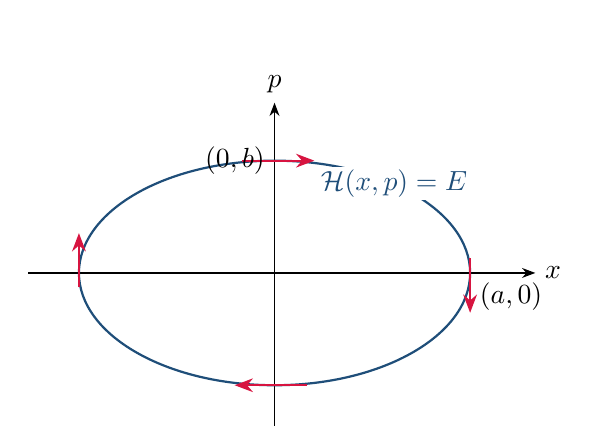
\begin{tikzpicture}[>=Stealth,scale=0.92]
  \draw[->] (-3.4,0) -- (3.6,0) node[right] {$x$};
  \draw[->] (0,-2.25) -- (0,2.35) node[above] {$p$};
  \draw[thick,noteBlue] (0,0) ellipse (2.7 and 1.55);
  \draw[->,thick,accentRed] (2.7,0.2) -- (2.7,-0.55);
  \draw[->,thick,accentRed] (-0.45,1.55) -- (0.55,1.55);
  \draw[->,thick,accentRed] (-2.7,-0.2) -- (-2.7,0.55);
  \draw[->,thick,accentRed] (0.45,-1.55) -- (-0.55,-1.55);
  \node[noteBlue,fill=white,inner sep=1pt] at (1.65,1.23)
    {$\mathcal H(x,p)=E$};
  \node[below right] at (2.7,0) {$(a,0)$};
  \node[left] at (0,1.55) {$(0,b)$};
\end{tikzpicture}

\textit{简谐振子的相空间能量椭圆。红色箭头由 Hamilton 正则方程决定；在右端点 $(a,0)$，$\dot p=-ka<0$，轨迹向下。}
\end{center}

完整推导见习题部分的\hyperref[exercise:QM-C02-S05-E00]{教材讲解例题}；练习 2.5.1--2.5.4 紧随其后。

\subsection{适用条件与常见误区}

\begin{itemize}[leftmargin=*]
  \item Hamiltonian 的定义是对速度变量的 Legendre 变换，不是把 $\mathcal L=T-V$ 中的负号机械改为正号。
  \item $\mathcal H$ 的最终表达式必须只含 $(q,p,t)$，不能遗留尚未消去的 $\dot q_i$。
  \item 普通 Hamilton 形式要求 $\dot q\mapsto p$ 可逆；速度 Hessian 奇异时不能直接套用本节推导。
  \item $\mathcal H=T+V$ 与 $\dd\mathcal H/\dd t=0$ 是两个不同命题，分别检查速度结构与显式时间依赖。
  \item 正则动量不一定等于机械动量；具体关系必须由 $p_i=\partial\mathcal L/\partial\dot q_i$ 计算。
  \item 二体系统总动量守恒只保证质心静止或匀速直线运动，不表示两个粒子之间没有相对运动。
\end{itemize}

\subsection{一分钟回顾}

Legendre 变换把广义速度替换为正则动量，使系统状态成为 $2n$ 维相空间中的点。Hamiltonian 的全微分与 Euler--Lagrange 方程共同给出 $\dot q_i=\partial\mathcal H/\partial p_i$、$\dot p_i=-\partial\mathcal H/\partial q_i$。对速度二次齐次、势能不依赖速度的标准系统，$\mathcal H=T+V$；若 Lagrangian 不显含时间，Hamiltonian 守恒。简谐振子在相空间中沿固定能量椭圆运动，显示 Hamiltonian 同时编码能量曲线与时间演化方向。

% 教材：Shankar, Principles of Quantum Mechanics, Second Edition
% 已覆盖：第 3 章第 3.1--3.5 节，印刷页 pp. 107--113，PDF pp. 120--126
% 人工核验：已完成分块讲解、问答和自编收口检查

\section{第 3.1 节：经典物理中的粒子与波}
\label{section:QM-C03-S01}

\studymeta
  {QM-C03-S01}
  {2026-09-04}
  {Shankar, \textit{Principles of Quantum Mechanics}, Second Edition}
  {第 3 章 \S 3.1；印刷页 pp.~107--108；PDF pp.~120--121}
  {讲解、自编检查与订正已完成}

\textbf{本节主线。}

经典物理把物质与辐射分别放入两套清楚分开的图景：粒子由有限个位置和动量变量描述，并沿确定轨迹运动；波则是定义在整个空间上的场，由波动方程控制。平面波把波长、周期、传播方向和强度压缩进振幅、频率与波矢。第三章将以这组经典区分为出发点，考察实验为何迫使我们修改它。

\notetopic{QM-C03-S01-T01}{经典粒子、经典波与初始数据}

\keyidea{粒子的状态由有限个数给出；波在固定时刻的状态是一整个空间函数。二者都需要与时间二阶运动方程相匹配的两组初始数据，但数据的类型不同。}

在经典粒子图景中，单个三维粒子在时刻 $t_0$ 的状态可由
\begin{equation}
  \bm r(t_0),\qquad \dot{\bm r}(t_0)
  \label{eq:QM-C03-S01-particle-initial-data}
\end{equation}
描述；在 Hamiltonian 形式中也可改用 $\bm r(t_0),\bm p(t_0)$。给定运动方程和初值后，原则上可确定一条轨迹 $\bm r(t)$。粒子的能量与动量被看作由局域对象携带；对有限个粒子，状态只需有限个自由度。

经典波则是分布在空间中的扰动。例如一维弦的位移由
\[
  \psi(x,t)
\]
描述：固定 $t$ 后，$x$ 是标记各空间位置的参数，而 $\psi(x,t)$ 给出每一点的场值。连续介质因此具有连续无穷多个自由度，不能用一个粒子坐标 $x(t)$ 代替整幅波形。

典型三维波动方程为
\begin{equation}
  \boxed{
  \nabla^2\psi(\bm r,t)
  =\frac{1}{c^2}
  \frac{\partial^2\psi(\bm r,t)}{\partial t^2}.}
  \label{eq:QM-C03-S01-wave-equation}
\end{equation}
由于它对时间是二阶方程，确定后续演化通常需要两个空间函数：
\begin{equation}
  \psi(\bm r,t_0),
  \qquad
  \left.\frac{\partial\psi(\bm r,t)}{\partial t}\right|_{t=t_0}.
  \label{eq:QM-C03-S01-wave-initial-data}
\end{equation}
它们分别是初始波形和每个空间点的初始变化率，对应粒子问题中的初始位置与初始速度。

只给初始波形一般不能确定传播方向。以一维波为例，
\begin{equation}
  \psi_+(x,t)=f(x-ct),
  \qquad
  \psi_-(x,t)=f(x+ct)
  \label{eq:QM-C03-S01-opposite-traveling-waves}
\end{equation}
在 $t=0$ 时都有 $\psi_\pm(x,0)=f(x)$，但
\[
  \dot\psi_+(x,0)=-cf'(x),
  \qquad
  \dot\psi_-(x,0)=cf'(x).
\]
前者向右、后者向左传播。相同初始形状配上不同初始速度，可以产生不同的后续运动。

\notetopic{QM-C03-S01-T02}{一维平面波、相位与传播速度}

一维简谐平面波可写成
\begin{align}
  \psi(x,t)
  &=A\exp\left[\ii\left(
    \frac{2\pi}{\lambda}x-
    \frac{2\pi}{T}t
  \right)\right] \notag\\
  &=\boxed{A\ee^{\ii(kx-\omega t)}},
  \label{eq:QM-C03-S01-plane-wave}
\end{align}
其中
\begin{equation}
  k=\frac{2\pi}{\lambda},
  \qquad
  \omega=\frac{2\pi}{T}.
  \label{eq:QM-C03-S01-k-omega-definitions}
\end{equation}
$k$ 是 wavenumber（波数或空间角频率），$\omega$ 是 angular frequency（角频率）。空间前进一个波长 $\lambda$ 或时间经过一个周期 $T$，相位都恰好改变 $2\pi$；因此 $k$ 与 $\omega$ 分别比 $1/\lambda$ 与 $1/T$ 多一个 $2\pi$。

波的相位为
\[
  \phi(x,t)=kx-\omega t.
\]
追踪某个固定相位点，令 $kx-\omega t=\phi_0$，则
\begin{equation}
  x(t)=\frac{\omega}{k}t+\frac{\phi_0}{k},
  \qquad
  v_{\mathrm{ph}}=\frac{\dd x}{\dd t}=\frac{\omega}{k}
  =\frac{\lambda}{T}.
  \label{eq:QM-C03-S01-phase-velocity}
\end{equation}
在 $k,\omega>0$ 的约定下，$\ee^{\ii(kx-\omega t)}$ 向 $+x$ 传播，而 $\ee^{\ii(kx+\omega t)}$ 向 $-x$ 传播。

把式~\eqref{eq:QM-C03-S01-plane-wave} 代入一维波动方程，可以直接得到频率与波数的关系：
\begin{align}
  \frac{\partial^2\psi}{\partial x^2}
  &=-k^2\psi,
  &
  \frac{\partial^2\psi}{\partial t^2}
  &=-\omega^2\psi.
  \label{eq:QM-C03-S01-plane-wave-second-derivatives}
\end{align}
因此
\begin{equation}
  -k^2\psi
  =-\frac{\omega^2}{c^2}\psi
  \quad\Longrightarrow\quad
  \boxed{\omega^2=c^2k^2}.
  \label{eq:QM-C03-S01-dispersion-relation}
\end{equation}
这个 $\omega$ 与 $k$ 的函数关系称为 dispersion relation（色散关系）。对正频率、向右传播的分支，$\omega=ck$，所以相速度就是 $c$。

\dialoguesupplement{与标准形式 $A\ee^{\ii(kx-\omega t)}$ 比较时，时间项的系数是 $-\omega$。例如 $3\ee^{\ii(4x-12t)}$ 对应 $k=4$、$\omega=12$，而不是 $\omega=-12$；周期和速率均取正值，传播方向由固定相位随时间的移动方向判断。}

\notetopic{QM-C03-S01-T03}{复数表示、强度与三维波矢}

真实的经典场通常取实值。若
\[
  A=\abs{A}\ee^{\ii\alpha},
\]
则复平面波的实部为
\begin{equation}
  \operatorname{Re}\psi(x,t)
  =\abs{A}\cos(kx-\omega t+\alpha),
  \label{eq:QM-C03-S01-real-wave}
\end{equation}
其中 $\alpha$ 是初相位。复指数是计算工具：微分只会产生 $\ii k$ 或 $-\ii\omega$ 因子。由于实系数波动方程是线性的，若复函数 $\psi=\psi_R+\ii\psi_I$ 是解，则实部 $\psi_R$ 与虚部 $\psi_I$ 分别也是解；计算结束后可取所需的实部。

教材采用
\begin{equation}
  I=\abs{\psi}^2
  \label{eq:QM-C03-S01-intensity}
\end{equation}
表示强度。对理想平面波，
\begin{equation}
  \abs{\psi(x,t)}^2
  =\abs{A}^2
   \abs{\ee^{\ii(kx-\omega t)}}^2
  =\boxed{\abs{A}^2},
  \label{eq:QM-C03-S01-plane-wave-intensity}
\end{equation}
因为复相位只在单位圆上转动而不改变模长。实际经典波的时间平均能流与振幅平方成正比；具体比例系数取决于所描述的物理场和归一化约定。

三维平面波写成
\begin{equation}
  \boxed{
  \psi(\bm r,t)
  =A\ee^{\ii(\bm k\cdot\bm r-\omega t)}},
  \qquad
  \abs{\bm k}=\frac{2\pi}{\lambda}.
  \label{eq:QM-C03-S01-three-dimensional-wave}
\end{equation}
$\bm k$ 是 wave vector（波矢）：它的模长给出空间相位变化率，方向给出传播方向。在固定时刻，等相位面满足
\begin{equation}
  \bm k\cdot\bm r=\text{常数}.
  \label{eq:QM-C03-S01-wavefront}
\end{equation}
因此 $\bm k$ 是等相位面的法向量，而单位法向量是
\[
  \widehat{\bm k}=\frac{\bm k}{\abs{\bm k}}.
\]
等相位面与 $\bm k$ 垂直，而不是平行。

\begin{figure}[htbp]
  \centering
  \begin{tikzpicture}[x=1.05cm,y=1.05cm,>=Latex]
    \foreach \x in {-2,-1,0,1,2}
      \draw[noteBlue,thick] (\x,-1.35)--(\x,1.35);
    \draw[->,very thick,accentRed] (-2.55,0)--(2.65,0)
      node[right] {$\bm k$};
    \node[noteBlue,align=center] at (0,1.75)
      {等相位面在二维截面中的投影};
    \draw[<->,verifyOrange] (0,-1.65)--(1,-1.65)
      node[midway,below] {$\lambda$};
  \end{tikzpicture}
  \caption{相邻波面相隔一个波长；波沿波矢所指的法向传播。}
  \label{fig:QM-C03-S01-wavefronts}
\end{figure}

三维相速度的大小为
\begin{equation}
  v_{\mathrm{ph}}=\frac{\omega}{\abs{\bm k}}.
  \label{eq:QM-C03-S01-three-dimensional-phase-velocity}
\end{equation}
本节只讨论单一平面波的相位传播；不同波数分量叠加后的波包及其传播将在后文需要时再区分处理。

\textbf{一分钟回顾。}

经典粒子由有限个位置与动量变量描述，经典波则由整个空间上的场函数描述。波动方程对时间为二阶，因此初始波形与初始变化率缺一不可。一维平面波 $A\ee^{\ii(kx-\omega t)}$ 的固定相位以 $\omega/k$ 向右传播，并满足 $\omega^2=c^2k^2$。复指数简化微分运算，实际场可取其实部；理想平面波强度为 $\abs{A}^2$。三维波矢 $\bm k$ 指向传播方向，并垂直于等相位面。

\section{第 3.2 节：经典波与经典粒子的双缝实验}
\label{section:QM-C03-S02}

\studymeta
  {QM-C03-S02}
  {2026-09-05}
  {Shankar, \textit{Principles of Quantum Mechanics}, Second Edition}
  {第 3 章 \S 3.2；印刷页 pp.~108--110；PDF pp.~121--123}
  {讲解、自编检查与订正已完成}

\textbf{本节主线。}

同一套双缝装置把经典波与经典粒子的组合规则清楚地区分开来：经典波先叠加复振幅，再取模平方得到强度，因此会出现干涉交叉项；彼此独立的经典粒子沿互斥路径到达探测器，因而直接相加概率或计数率。教材将在下一节用这两个经典基准检验光。

\notetopic{QM-C03-S02-T01}{经典波：振幅叠加、干涉项与条纹位置}

设两缝间距为 $d$，缝屏到探测屏的距离为 $D$，屏上观察点为 $X$，其纵坐标为 $x$；从两缝 $S_1,S_2$ 到 $X$ 的路程分别为 $r_1,r_2$。符号约定如图~\ref{fig:QM-C03-S02-double-slit-geometry} 所示。

\begin{figure}[htbp]
  \centering
  \begin{tikzpicture}[x=1.08cm,y=1.08cm,>=Latex]
    \foreach \y in {-1.5,-0.9,-0.3,0.3,0.9,1.5}
      \draw[->,noteBlue] (-2.0,\y)--(-0.25,\y);

    \draw[line width=1.8pt] (0,-2.0)--(0,-0.95);
    \draw[line width=1.8pt] (0,-0.55)--(0,0.55);
    \draw[line width=1.8pt] (0,0.95)--(0,2.0);
    \fill[accentRed] (0,0.75) circle (1.5pt)
      node[left=3pt] {$S_1$};
    \fill[accentRed] (0,-0.75) circle (1.5pt)
      node[left=3pt] {$S_2$};

    \draw[line width=1.3pt] (5,-2.0)--(5,2.0)
      node[above] {探测屏};
    \fill[verifyOrange] (5,1.35) circle (1.7pt)
      node[right=3pt] {$X$};
    \coordinate (O) at (5,0);
    \draw[densely dashed,noteBlue] (0,0.75)--(5,1.35)
      node[pos=0.57,above] {$r_1$};
    \draw[densely dashed,noteBlue] (0,-0.75)--(5,1.35)
      node[pos=0.57,below] {$r_2$};

    \draw[<->,verifyOrange] (0.38,-0.75)--(0.38,0.75)
      node[midway,right] {$d$};
    \draw[<->] (0,-2.25)--(5,-2.25)
      node[midway,below] {$D$};
    \draw[<->] (5.35,0)--(5.35,1.35)
      node[midway,right] {$x$};
    \draw[densely dotted] (0,0)--(O);
  \end{tikzpicture}
  \caption{双缝几何示意图。图为笔记自绘；远屏近轴近似要求 $D\gg d$ 且 $\abs{x}\ll D$。}
  \label{fig:QM-C03-S02-double-slit-geometry}
\end{figure}

只开 $S_1$ 时，屏上的复振幅和强度分别记作
\[
  \phi_1(x,t),
  \qquad
  I_1(x)=\abs{\phi_1(x,t)}^2;
\]
只开 $S_2$ 时同理得到 $\phi_2$ 与 $I_2$。两缝同时打开时，线性波动方程要求先叠加振幅：
\begin{equation}
  \phi_{1+2}=\phi_1+\phi_2.
  \label{eq:QM-C03-S02-amplitude-addition}
\end{equation}
所以强度为
\begin{align}
  I_{1+2}
  &=\abs{\phi_1+\phi_2}^2 \notag\\
  &=(\phi_1+\phi_2)^*(\phi_1+\phi_2) \notag\\
  &=\abs{\phi_1}^2+\abs{\phi_2}^2
    +\phi_1^*\phi_2+\phi_2^*\phi_1 \notag\\
  &=\boxed{I_1+I_2+2\operatorname{Re}(\phi_1^*\phi_2)}.
  \label{eq:QM-C03-S02-wave-interference}
\end{align}
最后两项是 interference term（干涉项）。这里必须保留复共轭；一般不能把干涉项写成 $\phi_1\phi_2$。

若两条波等振幅且同频，取
\begin{equation}
  \phi_j=A\ee^{\ii(kr_j-\omega t)},
  \qquad
  I_0=\abs{A}^2,
  \qquad
  \Delta r=r_2-r_1,
  \label{eq:QM-C03-S02-equal-amplitude-waves}
\end{equation}
则
\begin{align}
  I_{1+2}
  &=2I_0+2I_0\cos(k\Delta r) \notag\\
  &=\boxed{4I_0\cos^2\left(\frac{k\Delta r}{2}\right)}.
  \label{eq:QM-C03-S02-interference-intensity}
\end{align}
因此
\begin{align}
  \Delta r=n\lambda
  &\quad\Longrightarrow\quad
  I_{\max}=4I_0,
  \label{eq:QM-C03-S02-bright-condition}\\
  \Delta r=\left(n+\frac12\right)\lambda
  &\quad\Longrightarrow\quad
  I_{\min}=0,
  \label{eq:QM-C03-S02-dark-condition}
\end{align}
其中 $n\in\mathbb Z$。明纹对应同相叠加，暗纹对应反相抵消。

在 $D\gg d$ 且 $\abs{x}\ll D$ 的远屏近轴条件下，
\begin{equation}
  \Delta r\simeq d\sin\theta\simeq\frac{dx}{D}.
  \label{eq:QM-C03-S02-path-difference-approximation}
\end{equation}
代入明暗条件可得
\begin{align}
  x_n^{\mathrm{bright}}
  &\simeq \frac{n\lambda D}{d},
  &
  x_n^{\mathrm{dark}}
  &\simeq \frac{(n+\tfrac12)\lambda D}{d},
  \label{eq:QM-C03-S02-fringe-positions}
\end{align}
相邻明纹或暗纹的间距均为
\begin{equation}
  \boxed{\Delta x\simeq\frac{\lambda D}{d}}.
  \label{eq:QM-C03-S02-fringe-spacing}
\end{equation}
因此增大波长或屏距会拉宽条纹，增大缝距会压缩条纹。

\notetopic{QM-C03-S02-T02}{经典粒子：互斥路径的概率直接相加}

把入射波换成具有固定能量、方向有一定分布的经典粒子束。令 $P_1(x)$ 与 $P_2(x)$ 表示在相同入射条件下，粒子分别经 $S_1$、$S_2$ 落入 $x$ 附近同一探测区间的概率贡献；它们不是已经分别归一化为 $1$ 的条件分布。若探测的是单位时间内的粒子数，也可用相应计数率 $I_1(x),I_2(x)$ 表示相同的分布规律。

对每个经典粒子而言，“经 $S_1$ 到达 $x$”与“经 $S_2$ 到达 $x$”是 mutually exclusive（互斥）的两条路径。在两缝之间没有额外相互作用、粒子束条件保持不变的经典假设下，概率加法法则给出
\begin{equation}
  \boxed{P_{1+2}(x)=P_1(x)+P_2(x)},
  \qquad
  \boxed{I_{1+2}(x)=I_1(x)+I_2(x)}.
  \label{eq:QM-C03-S02-classical-particle-addition}
\end{equation}
这里没有类似式~\eqref{eq:QM-C03-S02-wave-interference} 的交叉项。$P_1P_2$ 描述两个事件同时发生时才可能出现的乘法结构，并不适用于“经 $S_1$ 或经 $S_2$”这一互斥选择。

即使两缝发出的粒子可能彼此碰撞，也可把入射强度降到一次只有一个粒子通过装置，从而排除粒子之间的相互影响。单次事件仍是某一个探测器的一次局域计数；重复足够多次后形成直方图，其平滑包络趋近 $I_1$、$I_2$ 或 $I_{1+2}$。在经典粒子模型中，由于 $P_2(x)\geq 0$，打开第二条路径不可能使某处的总到达概率低于只开第一条路径时的概率。

\notetopic{QM-C03-S02-T03}{实验判据与相干性边界}

两套经典预测的差别不在探测器是否逐点计数，而在组合规则：
\begin{equation}
  \boxed{
  \begin{aligned}
    \text{经典波：}&\quad
    \text{先加振幅，再取模平方};\\
    \text{经典粒子：}&\quad
    \text{对互斥路径直接加概率}.
  \end{aligned}}
  \label{eq:QM-C03-S02-two-composition-rules}
\end{equation}
经典波可以满足
\[
  I_{1+2}(x)\neq I_1(x)+I_2(x).
\]
特别是在干涉极小处，打开第二条缝反而可能降低该处的能流。经典粒子则必须满足式~\eqref{eq:QM-C03-S02-classical-particle-addition}，因此这种局部降低不可能出现。这是比“分布看起来有起伏”更直接的实验判据。

\dialoguesupplement{看不到稳定条纹并不足以单独证明对象服从经典粒子加法。若两束经典波的相对相位 $\delta$ 随时间或样本随机变化，则
\[
  I_{1+2}=I_1+I_2+2\sqrt{I_1I_2}\cos\delta.
\]
在相位均匀漂移且观测进行时间平均或系综平均时，$\langle\cos\delta\rangle=0$，于是 $\langle I_{1+2}\rangle=I_1+I_2$。瞬时干涉仍可能存在，只是缺乏稳定的相干关系，平均后不再形成可见条纹。}

\newpage
\textbf{一分钟回顾。}

双缝实验中，经典波先叠加振幅，再计算强度：
\[
  \phi_{1+2}=\phi_1+\phi_2,
  \qquad
  I_{1+2}=I_1+I_2+\phi_1^*\phi_2+\phi_2^*\phi_1.
\]
等振幅时强度为 $4I_0\cos^2(k\Delta r/2)$，远屏近轴下条纹间距为 $\lambda D/d$。经典粒子的两条路径互斥，故 $P_{1+2}=P_1+P_2$，不存在干涉项。打开第二缝能否降低某处的探测率，是区分两种经典组合规则的关键；但“没有稳定条纹”还可能来自经典波失去相干性，不能单独作为粒子性的充分证据。

\section{第 3.3 节：光的双缝实验}
\label{section:QM-C03-S03}

\studymeta
  {QM-C03-S03}
  {2026-09-06}
  {Shankar, \textit{Principles of Quantum Mechanics}, Second Edition}
  {第 3 章 \S 3.3；印刷页 pp.~110--112；PDF pp.~123--125}
  {讲解、自编检查与订正已完成}

\textbf{本节主线。}

光在双缝实验中同时表现出两类不能由同一套经典图景解释的现象：探测器每次记录一个局域、不可继续分割的能量转移事件，而大量这类事件累积出的空间分布却服从振幅叠加产生的干涉规律。量子理论因此不把光简单归入“经典粒子”或“经典波”，而是以概率振幅描述单次事件发生在各处的可能性。

\notetopic{QM-C03-S03-T01}{光的离散探测与光子能量、动量}

在强光下，探测器接收的能量看起来近似连续，经典电磁波的强度描述十分有效。把光强逐步降低并使用足够灵敏的探测器后，能量交换却表现为一次次局域计数，而不是任意小份额的连续沉积。每次计数所对应的电磁辐射量子称为 photon（光子）。

对角频率为 $\omega$、普通频率为 $\nu$ 的单色光，单个光子的能量由实验规律给出：
\begin{equation}
  \boxed{E=\hbar\omega=h\nu},
  \qquad
  \hbar=\frac{h}{2\pi},
  \qquad
  \omega=2\pi\nu.
  \label{eq:QM-C03-S03-photon-energy}
\end{equation}
光子的动量与波矢满足
\begin{equation}
  \boxed{\bm p=\hbar\bm k},
  \qquad
  p=\hbar k=\frac{h}{\lambda}.
  \label{eq:QM-C03-S03-photon-momentum}
\end{equation}
这里的 $E=\hbar\omega$ 与 $\bm p=\hbar\bm k$ 是由实验建立的量子关系，并不能只从经典波动方程推出。经典理论给出的 $\omega$、$\bm k$ 在量子描述中进一步决定单个光子的能量和动量。

真空中的光满足色散关系 $\omega=ck$，所以
\begin{equation}
  E=\hbar\omega
  =\hbar ck
  =pc.
  \label{eq:QM-C03-S03-photon-dispersion}
\end{equation}
与相对论能量--动量关系
\begin{equation}
  E^2=p^2c^2+m_0^2c^4
  \label{eq:QM-C03-S03-relativistic-energy-momentum}
\end{equation}
比较可知光子的静质量 $m_0=0$。这并不意味着光子没有能量或动量；它们分别由式~\eqref{eq:QM-C03-S03-photon-energy} 和式~\eqref{eq:QM-C03-S03-photon-momentum} 给出。

在理想单色光和固定探测效率的条件下，若平均每秒到达的光子数为 $\dot N$，平均功率为
\begin{equation}
  \boxed{\mathcal P=\dot N\hbar\omega}.
  \label{eq:QM-C03-S03-power-count-rate}
\end{equation}
因此在频率不变时降低光强，不会把每个光子的能量按比例削小，而会降低平均光子到达率。例如光强降为原来的 $1/5$ 时，单个光子的 $\hbar\omega$ 不变，单位时间内的平均计数降为原来的 $1/5$。若频率改变，则单个光子的能量也随 $\omega$ 改变。

\notetopic{QM-C03-S03-T02}{单光子双缝实验为何排除经典轨迹模型}

把入射光调弱到装置中平均一次只有一个光子，探测屏仍会记录一个个局域事件。短时间内这些点看似随机；经过大量重复后，计数直方图逐渐显现与经典波强度相同的干涉条纹。由于同一时刻没有第二个光子通过装置，条纹不能解释为不同光子之间碰撞或彼此扰动的结果。

经典粒子模型要得到
\begin{equation}
  N_{1+2}(x)=N_1(x)+N_2(x),
  \label{eq:QM-C03-S03-classical-count-addition}
\end{equation}
实际上需要同时采用两项假设：每个粒子经过 $S_1$ 或 $S_2$ 中一条确定路径；并且打开另一条缝不会改变原来那条路径对 $x$ 处计数的贡献。在这些假设下，两类事件互斥，故概率或平均计数率只能相加。

单光子实验却一般满足
\begin{equation}
  \boxed{\rho_{1+2}(x)\neq\rho_1(x)+\rho_2(x)},
  \label{eq:QM-C03-S03-nonclassical-probability-addition}
\end{equation}
其中 $\rho$ 表示单位长度内的探测概率密度。最直接的反例是理想暗纹位置 $x_0$。若两条路径在该处分别贡献
\begin{equation}
  \psi_1(x_0)=A,
  \qquad
  \psi_2(x_0)=-A,
  \label{eq:QM-C03-S03-dark-fringe-amplitudes}
\end{equation}
则只开任一条缝时的概率密度均为 $\abs{A}^2$，而两缝同时打开时
\begin{equation}
  \rho_{1+2}(x_0)
  =\abs{A-A}^2=0.
  \label{eq:QM-C03-S03-dark-fringe-probability}
\end{equation}
打开第二条缝反而把该处的探测概率从正值降为零，这与式~\eqref{eq:QM-C03-S03-classical-count-addition} 冲突。

这里排除的是“光子总有一条确定经典路径，而且另一条缝不影响该路径贡献”的独立轨迹模型。仅凭本节实验，不应把结论夸大为排除了所有可能含有轨迹概念的量子诠释。教材在此要确立的操作性事实是：实验结果不能由经典互斥概率直接相加得到，而必须先组合复概率振幅。

\notetopic{QM-C03-S03-T03}{概率振幅、Born 规则与统计条纹}

用态矢量 $\ket{\psi}$ 描述入射光的量子态。在连续位置基 $\{\ket{x}\}$ 中，
\begin{equation}
  \boxed{\psi(x)=\braket{x}{\psi}}
  \label{eq:QM-C03-S03-position-amplitude}
\end{equation}
是态矢量在 $\ket{x}$ 方向上的坐标，称为在位置 $x$ 探测到光子的 probability amplitude（概率振幅）。它本身一般是复数，不是概率，也不是经典电磁场能量密度。

Born 规则把振幅与可观测概率联系起来：
\begin{align}
  \Pr(x\leq X<x+\dd x)
  &=\abs{\psi(x)}^2\dd x,
  \label{eq:QM-C03-S03-born-infinitesimal}\\
  \Pr(a\leq X\leq b)
  &=\int_a^b\abs{\psi(x)}^2\dd x.
  \label{eq:QM-C03-S03-born-interval}
\end{align}
若光子必在整条探测屏上被发现，则态须满足归一化条件
\begin{equation}
  \int_{-\infty}^{\infty}\abs{\psi(x)}^2\dd x=1.
  \label{eq:QM-C03-S03-normalization}
\end{equation}
因此 $\abs{\psi(x)}^2$ 的量纲是长度的倒数，$\psi(x)$ 的量纲是 $\mathrm{length}^{-1/2}$。单点在连续空间中的概率通常为零；有物理意义的是有限区间概率或概率密度。

两缝同时打开时，量子理论使用与经典波相同形式的振幅叠加规则：
\begin{equation}
  \boxed{\psi_{1+2}(x)=\psi_1(x)+\psi_2(x)}.
  \label{eq:QM-C03-S03-amplitude-superposition}
\end{equation}
但这里的 $\psi_j$ 是到达 $x$ 的概率振幅。应用 Born 规则后，
\begin{align}
  \rho_{1+2}(x)
  &=\abs{\psi_1(x)+\psi_2(x)}^2 \notag\\
  &=\abs{\psi_1(x)}^2+\abs{\psi_2(x)}^2
    +\psi_1^*(x)\psi_2(x)+\psi_2^*(x)\psi_1(x) \notag\\
  &=\boxed{\rho_1(x)+\rho_2(x)
    +2\operatorname{Re}\!\left[\psi_1^*(x)\psi_2(x)\right]}.
  \label{eq:QM-C03-S03-born-interference}
\end{align}
交叉项可以为正也可以为负，所以打开第二条缝既可能增加、也可能降低某处的探测概率。

一次实验只产生一个完整、局域的探测事件；式~\eqref{eq:QM-C03-S03-born-interference} 预测的是这种事件在大量相同制备下的空间分布。若重复发送 $N$ 个同样制备的光子，则区间 $[a,b]$ 内计数的期望值为
\begin{equation}
  \boxed{
  \mathbb E\!\left[N_{[a,b]}\right]
  =N\int_a^b\abs{\psi(x)}^2\dd x.}
  \label{eq:QM-C03-S03-expected-counts}
\end{equation}
随着样本数增加，归一化直方图才逐渐逼近 $\abs{\psi(x)}^2$。因此“一个光子的一次探测”与“许多次探测形成干涉条纹”处在不同统计层次，并不矛盾。

\dialoguesupplement{为什么不直接把光视为经典波？经典波理论能准确给出许多实验中的平均干涉包络，但它把场能量视为可连续分割，不能单独解释探测器为何以局域的、能量为 $\hbar\omega$ 的完整事件响应。量子理论保留振幅的叠加结构，同时用 Born 规则把振幅模平方解释为单次事件的概率密度。}

\begin{figure}[htbp]
  \centering
  \begin{tikzpicture}[
    >=Latex,
    node distance=0.72cm and 0.65cm,
    box/.style={draw=noteBlue,rounded corners=2pt,align=center,
      minimum height=0.82cm,text width=2.55cm,fill=noteBlue!5},
    event/.style={draw=accentRed,rounded corners=2pt,align=center,
      minimum height=0.82cm,text width=2.35cm,fill=accentRed!5}
  ]
    \node[box] (state) {同一制备的\\单光子态 $\ket{\psi}$};
    \node[box,right=of state] (paths) {两条路径的振幅贡献\\$\psi_1(x),\ \psi_2(x)$};
    \node[box,right=of paths] (sum) {总振幅\\$\psi_1(x)+\psi_2(x)$};
    \node[event,right=of sum] (click) {一次完整的\\局域探测事件};
    \draw[->,thick] (state)--(paths);
    \draw[->,thick] (paths)--(sum);
    \draw[->,thick] (sum)--node[above] {$\abs{\cdot}^2$} (click);

    \node[box,below=1.0cm of sum] (repeat) {重复 $N$ 次\\独立制备与探测};
    \node[event,right=of repeat] (hist) {计数直方图\\$\propto\abs{\psi(x)}^2$};
    \draw[->,thick] (click)--(repeat);
    \draw[->,thick] (repeat)--(hist);
  \end{tikzpicture}
  \caption{单光子振幅叠加与统计条纹的层次。图为笔记自绘；两条振幅贡献不是把一个光子的能量分成两半。}
  \label{fig:QM-C03-S03-single-photon-statistics}
\end{figure}

\textbf{术语与适用边界。}
所谓“一个光子与自身干涉”只是对“同一单光子态的不同路径振幅在探测前相干叠加”的简称，不表示光子彼此碰撞，也不表示一次探测只吸收半个光子。更现代的表述把光子视为量子化电磁场的一次激发；本节的单光子概率波图景是进入量子公设前的物理动机，并不是完整的量子电动力学。严格的光子位置表象还存在超出本节范围的技术问题。

\textbf{一分钟回顾。}

光以局域、离散事件与物质交换能量和动量，每个光子满足 $E=\hbar\omega$、$\bm p=\hbar\bm k$，且真空中 $E=pc$。在固定频率下减弱光强，主要降低的是平均光子到达率，而非单个光子的能量。即使一次只有一个光子通过双缝，累计结果仍出现干涉，说明经典互斥路径概率不能直接相加。量子理论先叠加概率振幅 $\psi_1+\psi_2$，再由 Born 规则取模平方得到探测概率密度；单次结果是一个完整局域事件，大量重复才显现 $\abs{\psi(x)}^2$ 所规定的统计条纹。

\section{第 3.4 节：物质波（de Broglie 波）}
\label{section:QM-C03-S04}

\studymeta
  {QM-C03-S04}
  {2026-09-07}
  {Shankar, \textit{Principles of Quantum Mechanics}, Second Edition}
  {第 3 章 \S 3.4；印刷页 p.~112；PDF p.~125}
  {讲解、教材估算例、自编检查与订正已完成}

\textbf{本节主线。}

光原本被视为波，却以光子的形式携带离散的能量和动量。de Broglie 反向追问：传统上被视为粒子的电子等物质，是否也具有波动性？他的假设把粒子动量与波矢联系起来，并预言物质粒子同样可以发生干涉和衍射。宏观物体并非没有物质波，而是其波长和条纹间距通常小到无法由现实仪器分辨。

\notetopic{QM-C03-S04-T01}{de Broglie 假设与物质波的概率解释}

de Broglie hypothesis（德布罗意假设）认为，动量为 $\bm p$ 的粒子对应波矢 $\bm k$，满足
\begin{equation}
  \boxed{\bm p=\hbar\bm k}.
  \label{eq:QM-C03-S04-de-broglie-vector}
\end{equation}
因此 $\bm k$ 与 $\bm p$ 同向，而且
\begin{equation}
  k=\frac{p}{\hbar}.
  \label{eq:QM-C03-S04-wave-number}
\end{equation}
结合 $k=2\pi/\lambda$ 和 $h=2\pi\hbar$，得到 de Broglie wavelength（德布罗意波长）
\begin{align}
  \frac{2\pi}{\lambda}
  &=\frac{p}{\hbar},
  \notag\\
  \boxed{\lambda=\frac{2\pi\hbar}{p}=\frac{h}{p}}.
  \label{eq:QM-C03-S04-de-broglie-wavelength}
\end{align}
真正普遍的关系是 $\lambda=h/p$。只有在非相对论条件下，才可再用 $p=mv$ 写成
\begin{equation}
  \boxed{\lambda=\frac{h}{mv}}.
  \label{eq:QM-C03-S04-nonrelativistic-wavelength}
\end{equation}
速度接近光速时必须使用相对论动量，不能继续把 $p$ 简写为 $mv$。

式~\eqref{eq:QM-C03-S04-de-broglie-wavelength} 给出两个直接判断：
\begin{itemize}[leftmargin=*]
  \item 对同一种粒子，动量越大，波长越短；
  \item 两个粒子若动量大小相同，则 de Broglie 波长相同；若非相对论速度相同，则质量越大的粒子波长越短。
\end{itemize}

Davisson--Germer experiment（戴维孙--革末实验）观察到了电子衍射，从实验上验证了电子的波数与动量服从 $k=p/\hbar$。物质波并不表示电子沿波浪形轨迹前进，也不应被解释为连续摊开的经典物质密度。教材沿用上一节的概率解释，以
\begin{equation}
  \psi(x,t)
  \label{eq:QM-C03-S04-matter-wave-amplitude}
\end{equation}
表示在时刻 $t$ 于位置 $x$ 探测到粒子的 probability amplitude（概率振幅），而
\begin{equation}
  \boxed{
  \Pr(x\leq X<x+\dd x)
  =\abs{\psi(x,t)}^2\dd x}
  \label{eq:QM-C03-S04-matter-wave-born-rule}
\end{equation}
才是相应的位置概率。

在双缝实验中，两条路径贡献的概率振幅先相加：
\begin{equation}
  \psi_{1+2}(x)=\psi_1(x)+\psi_2(x),
  \label{eq:QM-C03-S04-matter-wave-superposition}
\end{equation}
于是
\begin{equation}
  \abs{\psi_{1+2}(x)}^2
  =\abs{\psi_1(x)}^2+\abs{\psi_2(x)}^2
   +2\operatorname{Re}\!\left[\psi_1^*(x)\psi_2(x)\right].
  \label{eq:QM-C03-S04-matter-wave-interference}
\end{equation}
单个粒子仍只在屏上产生一次局域探测；大量同样制备的粒子才累积出由式~\eqref{eq:QM-C03-S04-matter-wave-interference} 描述的干涉分布。

\dialoguesupplement{本节所排除的是朴素经典模型：粒子经过一条确定且不受另一条缝影响的路径，两条互斥路径的概率直接相加。仅凭这里的论证，不应把结论扩大为排除一切含“轨迹”概念的量子诠释。}

\notetopic{QM-C03-S04-T02}{宏观经典极限：极短波长与不可分辨条纹}

教材考虑质量为 $1\,\mathrm{g}$、速度为 $1\,\mathrm{cm/s}$ 的弹丸。在非相对论条件下，
\begin{equation}
  p=mv
  =1\,\mathrm{g\,cm/s}.
  \label{eq:QM-C03-S04-pellet-momentum}
\end{equation}
使用
\[
  h\simeq
  6.626\times10^{-27}\,
  \mathrm{g\,cm^2/s},
\]
得到
\begin{align}
  \lambda
  &=\frac{h}{p}
    =\frac{6.626\times10^{-27}\,
      \mathrm{g\,cm^2/s}}
      {1\,\mathrm{g\,cm/s}}
  \notag\\
  &=6.626\times10^{-27}\,\mathrm{cm}
    \sim\boxed{10^{-26}\,\mathrm{cm}}.
  \label{eq:QM-C03-S04-pellet-wavelength}
\end{align}
教材指出，这比质子半径还小约 $10^{13}$ 倍。如此短的波长并不等于“没有物质波”，而意味着相应的干涉结构极其细密。

对远屏近轴双缝装置，条纹间距近似为
\begin{equation}
  \boxed{\Delta x\simeq\frac{\lambda D}{d}},
  \label{eq:QM-C03-S04-fringe-spacing}
\end{equation}
其中 $D$ 是双缝到屏幕的距离，$d$ 是缝间距。$\lambda$ 越短，$\Delta x$ 也越小。

实际探测器具有有限的空间分辨率。若一个像素覆盖宽度 $\delta x$，它记录的是区间概率
\begin{equation}
  P_{\mathrm{pixel}}
  =\int_{x_0}^{x_0+\delta x}
   \abs{\psi_{1+2}(x)}^2\dd x,
  \label{eq:QM-C03-S04-pixel-probability}
\end{equation}
而不是数学上无限精确的点值。当
\begin{equation}
  \delta x\gg\Delta x
  \label{eq:QM-C03-S04-unresolved-condition}
\end{equation}
时，一个像素内部包含许多明暗条纹。若 $\abs{\psi_1}$、$\abs{\psi_2}$ 的包络在该像素内变化缓慢，快速振荡的交叉项会近似平均为零：
\begin{equation}
  \int_{x_0}^{x_0+\delta x}
  2\operatorname{Re}\!\left[\psi_1^*(x)\psi_2(x)\right]\dd x
  \simeq0.
  \label{eq:QM-C03-S04-cross-term-average}
\end{equation}
因此仪器看到的粗粒化分布近似满足
\begin{equation}
  \boxed{
  \overline{\rho}_{1+2}(x)
  \simeq\rho_1(x)+\rho_2(x),}
  \label{eq:QM-C03-S04-classical-coarse-graining}
\end{equation}
与经典粒子预测相同。这里消失的是仪器可分辨的干涉条纹，而不是物质波关系本身。

\begin{figure}[htbp]
  \centering
  \begin{tikzpicture}[>=Latex,node distance=0.8cm and 0.7cm,
    box/.style={draw=noteBlue,rounded corners=2pt,align=center,
      minimum height=0.9cm,text width=2.55cm,fill=noteBlue!5},
    result/.style={draw=accentRed,rounded corners=2pt,align=center,
      minimum height=0.9cm,text width=2.7cm,fill=accentRed!5}]
    \node[box] (p) {宏观动量 $p$ 很大};
    \node[box,right=of p] (lambda) {$\lambda=h/p$\\极小};
    \node[box,right=of lambda] (fringe) {$\Delta x\simeq\lambda D/d$\\极小};
    \node[result,right=of fringe] (average) {有限分辨率平均\\干涉交叉项};
    \draw[->,thick] (p)--(lambda);
    \draw[->,thick] (lambda)--(fringe);
    \draw[->,thick] (fringe)--(average);
  \end{tikzpicture}
  \caption{本节给出的宏观经典极限。图为笔记自绘；经典分布来自不可分辨条纹的粗粒化平均，而非先验删除物质波。}
  \label{fig:QM-C03-S04-macroscopic-limit}
\end{figure}

\textbf{适用边界。}
上述“条纹过密而被平均”的解释就是教材本节采用的论证。现实宏观物体还会与环境强烈耦合，decoherence（退相干）也会抑制可观测干涉；这属于后续量子理论内容，不是本节推导的前提。

\textbf{一分钟回顾。}

de Broglie 假设把物质粒子的动量与波矢联系为 $\bm p=\hbar\bm k$，因而 $\lambda=h/p$；非相对论时才可进一步写成 $h/(mv)$。物质波 $\psi(x,t)$ 是概率振幅，而不是经典物质密度或波浪形轨迹。单个粒子产生局域探测，大量重复实验通过振幅交叉项形成干涉分布。宏观物体的动量很大，故 $\lambda$ 与双缝条纹间距都极小；当仪器分辨率远大于条纹间距时，交叉项被粗粒化平均，最终呈现近似经典的概率相加规律。

\section{第 3.5 节：结论}
\label{section:QM-C03-S05}

\studymeta
  {QM-C03-S05}
  {2026-09-08}
  {Shankar, \textit{Principles of Quantum Mechanics}, Second Edition}
  {第 3 章 \S 3.5；印刷页 pp.~112--113；PDF pp.~125--126}
  {讲解、自编检查与订正已完成}

\textbf{本节主线。}

第三章并未给出完整的量子理论，而是用双缝实验说明经典粒子与经典波两套图景都不足以单独描述电子、光子等量子对象。量子对象在探测时呈现局域、完整的事件，却在重复实验的统计分布中呈现概率振幅的叠加与干涉。由此需要用波函数或抽象态矢量描述状态，并把状态随时间的变化作为量子动力学的核心问题；这些经验事实将在下一章被组织成量子力学公设。

\notetopic{QM-C03-S05-T01}{波粒二象性的操作性内容}

量子对象的 particlelike（粒子性）首先体现在单次探测：电子或光子在屏幕上的某个确定位置触发一次局域事件，并在该事件中传递完整的能量、动量与电荷。一次结果可以写成
\begin{equation}
  X=x_{\mathrm{det}},
  \label{eq:QM-C03-S05-local-detection}
\end{equation}
但“探测位置确定”并不推出探测前存在一条确定的经典轨迹。

其 wavelike（波动性）则体现在概率振幅的组合规律。若到达同一位置 $x$ 的两种不可区分选择分别贡献 $\psi_1(x,t)$ 与 $\psi_2(x,t)$，则
\begin{align}
  \psi(x,t)
  &=\psi_1(x,t)+\psi_2(x,t),
  \label{eq:QM-C03-S05-amplitude-sum}\\
  \rho(x,t)
  &=\abs{\psi(x,t)}^2 \notag\\
  &=\abs{\psi_1(x,t)}^2+\abs{\psi_2(x,t)}^2
    +2\operatorname{Re}\!\left[\psi_1^*(x,t)\psi_2(x,t)\right].
  \label{eq:QM-C03-S05-interference-density}
\end{align}
交叉项使累计分布不能由两条经典互斥路径的概率直接相加得到。对单个粒子，位置测量的 Born 规则为
\begin{equation}
  \boxed{
  \Pr(a\leq X\leq b;t)
  =\int_a^b\abs{\psi(x,t)}^2\dd x.}
  \label{eq:QM-C03-S05-position-born-rule}
\end{equation}
因此 $\psi(x,t)$ 与每个粒子的量子态相关，而不是只有许多粒子组成的束流才拥有的经典波。一次实验给出一个位置；大量相同制备的实验才使归一化计数分布趋近 $\abs{\psi(x,t)}^2$。

wave--particle duality（波粒二象性）不应理解为量子对象在“经典小球”和“经典连续波”之间来回变形。更准确的说法是：不同实验分别显露出与两种经典图景相似的特征，但量子态本身不等同于任何一种经典对象。

\dialoguesupplement{教材在此排除的是朴素的经典确定路径模型：粒子预先选择一条不受另一条缝影响的路径，且两条路径的普通概率直接相加。仅凭本章实验，不应把结论扩大为排除所有带有轨迹概念的量子诠释。}

\notetopic{QM-C03-S05-T02}{从位置波函数到抽象状态及其动力学}

教材把粒子的状态写成位置波函数 $\psi(x,t)$，也写成抽象 ket $\ket{\psi(t)}$。二者不是两个状态，而满足
\begin{equation}
  \boxed{\psi(x,t)=\braket{x}{\psi(t)}}.
  \label{eq:QM-C03-S05-position-component}
\end{equation}
$\ket{\psi(t)}$ 是不依赖所选基的抽象态矢量；$\psi(x,t)$ 是它在连续位置基 $\{\ket{x}\}$ 下的坐标。利用完备关系
\begin{equation}
  \int_{-\infty}^{\infty}\ket{x}\bra{x}\dd x=I,
  \label{eq:QM-C03-S05-position-completeness}
\end{equation}
可以反向重建
\begin{align}
  \ket{\psi(t)}
  &=I\ket{\psi(t)} \notag\\
  &=\int_{-\infty}^{\infty}
    \ket{x}\braket{x}{\psi(t)}\dd x \notag\\
  &=\boxed{
    \int_{-\infty}^{\infty}
    \psi(x,t)\ket{x}\dd x}.
  \label{eq:QM-C03-S05-state-reconstruction}
\end{align}
这正是有限维展开 $\ket{v}=\sum_i\ket{i}\braket{i}{v}$ 的连续版本。

经典力学与量子力学的动力学问题可作如下对照：
\begin{center}
\begin{tabularx}{0.94\textwidth}{@{}>{\raggedright\arraybackslash}p{2.6cm}XX@{}}
  \toprule
  & 经典力学 & 量子力学的初步图景 \\
  \midrule
  状态 & 相空间点 $(x(t),p(t))$ & 态矢量 $\ket{\psi(t)}$ \\
  位置描述 & 确定位置 $x(t)$ & 振幅 $\psi(x,t)=\braket{x}{\psi(t)}$ \\
  位置预测 & 理想情况下由轨迹确定 & $\abs{\psi(x,t)}^2$ 给出概率密度 \\
  动力学问题 & 求 $(x(0),p(0))\mapsto(x(t),p(t))$ & 求 $\ket{\psi(0)}\mapsto\ket{\psi(t)}$ \\
  \bottomrule
\end{tabularx}
\end{center}

只知道某一组测量结果的概率通常不足以确定状态。例如对离散正交基 $\{\ket{1},\ket{2}\}$，
\begin{equation}
  \ket{\phi_+}=\frac{\ket{1}+\ket{2}}{\sqrt2},
  \qquad
  \ket{\phi_-}=\frac{\ket{1}-\ket{2}}{\sqrt2}
  \label{eq:QM-C03-S05-relative-phase-states}
\end{equation}
在该基下都给出 $P(1)=P(2)=1/2$，但相对相位不同，换到干涉基后即可区分。这说明概率振幅包含比单组概率更多的信息。

第三章的双缝实验提供了量子公设的物理动机，却不能单独推出量子理论的全部结构。下一章将进一步规定 $\ket{\psi(t)}$ 包含哪些可观测信息、测量如何产生结果，以及状态怎样随时间演化。

\textbf{离散概率与连续概率密度。}
若测量基是离散的 $\{\ket{n}\}$，则
\begin{equation}
  \boxed{P(n)=\abs{\braket{n}{\psi}}^2},
  \qquad
  \sum_nP(n)=1,
  \label{eq:QM-C03-S05-discrete-born-rule}
\end{equation}
这里的 $P(n)$ 是 probability mass（离散概率），不需要积分。若测量位置这一连续变量，则 $\abs{\psi(x)}^2$ 是 probability density（概率密度），有限区间概率必须按式~\eqref{eq:QM-C03-S05-position-born-rule} 积分。不能把连续空间中某一点的密度值直接当作该点的概率。

\textbf{一分钟回顾。}

量子对象在单次探测中以完整的局域事件出现，但其重复实验分布必须由概率振幅的叠加与 Born 规则计算；这就是本章所说波粒二象性的操作性内容。抽象态 $\ket{\psi(t)}$ 与位置波函数由 $\psi(x,t)=\braket{x}{\psi(t)}$ 联系，后者只是前者在位置基中的坐标。量子动力学研究的是整个状态 $\ket{\psi(t)}$ 如何演化，而不是预设一条经典确定轨迹。双缝实验为这些结构提供动机，但完整公设仍需由下一章正式给出。

% 教材：Shankar, Principles of Quantum Mechanics, Second Edition
% 已覆盖：第 4 章第 4.1--4.2 节，印刷页 pp. 115--143，PDF pp. 127--155
% 人工核验：已完成分块讲解、教材练习 4.2.1--4.2.3 与订正

\clearpage
\section{第 4.1 节：量子力学公设}
\label{section:QM-C04-S01}

\studymeta
  {QM-C04-S01}
  {2026-09-08}
  {Shankar, \textit{Principles of Quantum Mechanics}, Second Edition}
  {第 4 章 \S 4.1；印刷页 pp.~115--116；PDF pp.~127--128}
  {讲解、教材练习 4.2.1 与订正已完成}

\textbf{本节主线。}

前两章分别建立了 Hilbert 空间与经典 Hamiltonian 力学，第三章则说明经典粒子和经典波都不足以单独描述量子实验。第 4.1 节把这些数学工具和实验约束压缩为四条公设：状态由什么表示、物理量由什么表示、测量给出什么结果，以及状态怎样随时间变化。

\textbf{来源边界。}四条公设及其经典对应来自教材第 4.1 节。教材在第 1.10 节讨论了 $X$、$K$ 与 Fourier 变换，在第 3.4 节给出 $p=\hbar k$ 的物理动机，但没有在本节完整重建这些公设的历史发现过程。下文标为“对话补充”的平移生成元、平面波和 Hamiltonian 辨析，是理解公设的辅助推导，不是从经典力学严格证明量子力学。

\begin{figure}[htbp]
  \centering
  \begin{tikzpicture}[
    node distance=0.8cm and 1.0cm,
    box/.style={draw=noteBlue,rounded corners=2pt,align=center,
      minimum height=1.0cm,text width=5.25cm,fill=noteBlue!5},
    arrow/.style={->,thick,>=Latex}]
    \node[box] (state) {公设 I：状态\\$\ket{\psi(t)}\in\hilbert$};
    \node[box,right=of state] (observable) {公设 II：可观测量\\$\omega(x,p)\mapsto\Omega(X,P)$};
    \node[box,below=of observable] (measurement) {公设 III：测量\\本征值、Born 概率与投影更新};
    \node[box,left=of measurement] (dynamics) {公设 IV：动力学\\$\ii\hbar\,\dd\ket{\psi}/\dd t=H\ket{\psi}$};
    \draw[arrow] (state)--(observable);
    \draw[arrow] (observable)--(measurement);
    \draw[arrow] (state)--(dynamics);
    \draw[arrow] (dynamics)--(measurement);
  \end{tikzpicture}
  \caption{四条公设的逻辑分工。图为笔记自绘：公设 I 给出状态对象，公设 II 与 III 从状态提取实验预测，公设 IV 给出不测量时的时间演化。}
  \label{fig:QM-C04-S01-four-postulates}
\end{figure}

\notetopic{QM-C04-S01-T01}{公设 I：状态是 Hilbert 空间中的射线}

\keyidea{量子态由 Hilbert 空间中的非零 ket 表示；归一化 ket 便于直接读取绝对概率，但真正的物理纯态是相差非零复数倍的一条射线。}

在给定时刻，粒子的状态由
\begin{equation}
  \boxed{\ket{\psi(t)}\in\hilbert}
  \label{eq:QM-C04-S01-state-postulate}
\end{equation}
表示。选取离散正交归一基 $\{\ket{i}\}$ 后，
\begin{equation}
  \ket{\psi(t)}
  =\sum_i\ket{i}\braket{i}{\psi(t)}.
  \label{eq:QM-C04-S01-discrete-state-expansion}
\end{equation}
在连续位置基中，同一个抽象态写成
\begin{align}
  \psi(x,t)&=\braket{x}{\psi(t)},
  \label{eq:QM-C04-S01-position-wavefunction}\\
  \ket{\psi(t)}
  &=\int_{-\infty}^{\infty}
    \psi(x,t)\ket{x}\dd x.
  \label{eq:QM-C04-S01-position-reconstruction}
\end{align}
$\psi(x,t)$ 是抽象态在位置基下的坐标，不是与 $\ket{\psi(t)}$ 不同的第二个物理状态。

对 proper state（可正规化态），通常取
\begin{equation}
  \braket{\psi}{\psi}=1.
  \label{eq:QM-C04-S01-normalization}
\end{equation}
零向量的范数始终为零，不能通过乘常数变成归一化态，因此不代表物理纯态。若 $c\neq0$，则 $\ket{\psi}$ 与 $c\ket{\psi}$ 给出相同的归一化测量概率；归一化以后仍可乘整体相位：
\begin{equation}
  \ket{\psi}\sim\ee^{\ii\alpha}\ket{\psi}.
  \label{eq:QM-C04-S01-global-phase-equivalence}
\end{equation}
所有分量共同获得的 global phase（整体相位）不可观测；不同分量之间的 relative phase（相对相位）通常能够改变另一测量基中的概率。

Hilbert 空间的线性结构给出 superposition principle（叠加原理）：若 $\ket{\psi}$ 与 $\ket{\phi}$ 是允许状态，则非零线性组合
\[
  a\ket{\psi}+b\ket{\phi}
\]
经归一化后也是允许状态。叠加态不是“系统暗中处于其中一个状态但我们不知道”，因为相对相位能够通过干涉测量显现。

\notetopic{QM-C04-S01-T02}{公设 II：可观测量与 Hermitian 算符}

\keyidea{经典 dynamical variable $\omega(x,p)$ 在量子理论中由 Hermitian 算符 $\Omega(X,P)$ 表示。矩阵或微分表达式只是该抽象算符在某一组基下的表示。}

教材给出基本位置、动量算符在位置本征基中的积分核：
\begin{align}
  \bra{x}X\ket{x'}
  &=x\,\delta(x-x'),
  \label{eq:QM-C04-S01-X-kernel}\\
  \bra{x}P\ket{x'}
  &=-\ii\hbar\,\delta'(x-x').
  \label{eq:QM-C04-S01-P-kernel}
\end{align}
因此它们对位置波函数的作用为
\begin{align}
  \bra{x}X\ket{\psi}
  &=x\psi(x),
  \label{eq:QM-C04-S01-X-action}\\
  \bra{x}P\ket{\psi}
  &=-\ii\hbar\frac{\dd\psi}{\dd x}.
  \label{eq:QM-C04-S01-P-action}
\end{align}
第一式来自 $X\ket{x}=x\ket{x}$；第二式中的导数算符不是凭矩阵运算“算出来”的物理定律，而是数学结构与实验关系共同锁定的表示。

\dialoguesupplement{第 1.10 节中的 wave-number operator 为 $K=-\ii\,\dd/\dd x$。平面波满足
\[
  K\ee^{\ii kx}=k\ee^{\ii kx}.
\]
第 3.4 节的 de Broglie 关系 $p=\hbar k$ 于是把 $K$ 的本征值 $k$ 对应到动量 $p$，给出 $P=\hbar K=-\ii\hbar\,\dd/\dd x$。同一结论也可由空间平移得到：主动平移 $a$ 后，$\psi_a(x)=\psi(x-a)=\psi(x)-a\psi'(x)+O(a^2)$；而连续幺正平移写成 $T(a)=I-\ii aP/\hbar+O(a^2)$。比较一阶项即得 $P\psi=-\ii\hbar\psi'$。这里真正的物理识别是“动量生成空间平移”；求导形式是该识别在位置表象中的数学结果。}

一般经典变量按
\begin{equation}
  \omega(x,p)\longmapsto\Omega(X,P)
  \label{eq:QM-C04-S01-quantization-map}
\end{equation}
构造。若 $\omega$ 同时含 $x,p$，经典乘法可交换而量子算符一般不交换，故可能出现 ordering ambiguity（排序歧义）。例如 $xp=px$ 在经典理论中是同一个函数，但 $XP\neq PX$；常见 Hermitian 选择是
\begin{equation}
  xp\longmapsto\frac12(XP+PX).
  \label{eq:QM-C04-S01-symmetric-ordering}
\end{equation}
这不是普适唯一规则；真正有歧义时还需额外物理原则或实验决定。

\textbf{三种逻辑层次。}
\begin{center}
\begin{tabularx}{0.95\textwidth}{@{}>{\raggedright\arraybackslash}p{2.5cm}X@{}}
  \toprule
  层次 & 本节中的典型内容 \\
  \midrule
  数学定义 & $X\ket{x}=x\ket{x}$；选定 Hilbert 空间、基与算符 \\
  数学后果 & $\bra{x}X\ket{\psi}=x\psi(x)$；平移生成元在位置表象中表现为导数 \\
  物理识别或公设 & $p=\hbar k$、动量生成平移、Hermitian 算符代表可观测量 \\
  \bottomrule
\end{tabularx}
\end{center}
不能把第三层说成由纯数学必然推出；数学负责保证结构自洽，实验与对应原理负责判断这套结构是否描述现实。

\notetopic{QM-C04-S01-T03}{公设 III：测量、本征值与 Born 规则}

\keyidea{理想测量的可能结果是可观测算符的本征值；概率由态在对应本征子空间上的投影模平方给出，测量后状态更新为该归一化投影。}

设 Hermitian 算符 $\Omega$ 的谱分解为
\begin{equation}
  \Omega=\sum_\omega\omega\Pi_\omega,
  \label{eq:QM-C04-S01-spectral-decomposition}
\end{equation}
其中 $\Pi_\omega$ 投影到本征值 $\omega$ 的完整本征子空间。对归一化初态 $\ket{\psi}$，理想测量满足
\begin{align}
  \text{可能结果}&:\quad \omega,
  \label{eq:QM-C04-S01-measurement-outcomes}\\
  P(\omega)
  &=\boxed{\bra{\psi}\Pi_\omega\ket{\psi}},
  \label{eq:QM-C04-S01-born-projector}\\
  \ket{\psi}
  &\longrightarrow
  \boxed{
  \frac{\Pi_\omega\ket{\psi}}
       {\sqrt{\bra{\psi}\Pi_\omega\ket{\psi}}}}
  \quad\text{若得到 }\omega.
  \label{eq:QM-C04-S01-state-update}
\end{align}
若 $\omega$ 非简并，$\Pi_\omega=\ket{\omega}\bra{\omega}$，于是
\[
  P(\omega)=\abs{\braket{\omega}{\psi}}^2.
\]
若 $\omega$ 简并，必须投影到整个本征子空间，不能在没有额外测量信息时擅自选定其中某一个本征向量。

算符作用
\begin{equation}
  \Omega\ket{\psi}
  =\sum_\omega\omega\Pi_\omega\ket{\psi}
  \label{eq:QM-C04-S01-operator-action-not-measurement}
\end{equation}
是确定性的线性运算，一般仍是叠加态，也未必归一化；它不是“一次实际测量”。测量则随机给出某个本征值，并按式~\eqref{eq:QM-C04-S01-state-update} 更新状态。

测量的 expectation value（期望值）为
\begin{equation}
  \boxed{\langle\Omega\rangle
  =\bra{\psi}\Omega\ket{\psi}}
  =\sum_\omega\omega P(\omega),
  \label{eq:QM-C04-S01-expectation}
\end{equation}
它是大量同样制备系统的测量平均，不要求等于某次测量可以取得的本征值。相应 uncertainty（不确定度）为
\begin{equation}
  \boxed{
  \Delta\Omega
  =\sqrt{\langle\Omega^2\rangle-\langle\Omega\rangle^2}}.
  \label{eq:QM-C04-S01-uncertainty}
\end{equation}

连续谱中，$\abs{\braket{\omega}{\psi}}^2$ 是 probability density（概率密度），有限区间概率才是
\begin{equation}
  \Pr(a\leq\Omega\leq b)
  =\int_a^b\abs{\braket{\omega}{\psi}}^2\dd\omega.
  \label{eq:QM-C04-S01-continuous-born-rule}
\end{equation}
离散概率可以直接相加，连续概率密度必须积分；二者不能混用。

本节测量规则的代表性计算见\relatedexercise{QM-C04-S01-E01}{教材练习 4.2.1}。

\notetopic{QM-C04-S01-T04}{公设 IV：Schrödinger 方程与 Hamiltonian}

\keyidea{封闭量子系统在不发生测量时按 Schrödinger 方程作幺正演化。Hamiltonian 的首要结构角色是时间平移生成元；在本节采用的标准非相对论系统中，它同时代表总能量。}

量子态的动力学由
\begin{equation}
  \boxed{
  \ii\hbar\frac{\dd}{\dd t}\ket{\psi(t)}
  =H(t)\ket{\psi(t)}}
  \label{eq:QM-C04-S01-schrodinger-abstract}
\end{equation}
给出。对于一维标准 Hamiltonian
\begin{equation}
  H=\frac{P^2}{2m}+V(X),
  \label{eq:QM-C04-S01-standard-hamiltonian}
\end{equation}
投影到位置基得到
\begin{equation}
  \boxed{
  \ii\hbar\frac{\partial\psi(x,t)}{\partial t}
  =\left[-\frac{\hbar^2}{2m}\frac{\partial^2}{\partial x^2}
    +V(x,t)\right]\psi(x,t)}.
  \label{eq:QM-C04-S01-schrodinger-position}
\end{equation}

若 $H$ 与时间无关且为 self-adjoint（自伴）算符，则
\begin{equation}
  \ket{\psi(t)}
  =U(t,t_0)\ket{\psi(t_0)},
  \qquad
  U(t,t_0)=\ee^{-\ii H(t-t_0)/\hbar},
  \label{eq:QM-C04-S01-time-evolution-operator}
\end{equation}
且 $U^\dagger U=I$，故范数保持不变。若
\[
  H\ket{E_n}=E_n\ket{E_n},
\]
则能量本征态只获得整体相位：
\begin{equation}
  \ket{E_n,t}
  =\ee^{-\ii E_n(t-t_0)/\hbar}\ket{E_n}.
  \label{eq:QM-C04-S01-energy-eigenstate-evolution}
\end{equation}
一般叠加态的不同能量分量则积累不同相位，relative phase 随时间改变并影响后续测量。

\dialoguesupplement{Schrödinger 方程可获得强烈但非严格的平面波动机。对 $\psi=A\ee^{\ii(kx-\omega t)}$，Planck--Einstein 与 de Broglie 关系给出 $E=\hbar\omega$、$p=\hbar k$，因此
\[
  \ii\hbar\partial_t\psi=E\psi,
  \qquad
  -\ii\hbar\partial_x\psi=p\psi.
\]
把经典非相对论关系 $E=p^2/(2m)+V$ 中的 $E,p$ 替换为这些算符，可得到式~\eqref{eq:QM-C04-S01-schrodinger-position}。这说明公式为何自然，却不能证明自然界必须服从它；普适有效性仍是由实验检验的物理公设。}

\textbf{Hamiltonian 与能量的区别。}
在教材当前采用的惯性参考系、标准闭合非相对论系统中，公设 II 把经典能量 $\mathcal H(x,p)$ 映射为能量算符 $H(X,P)$，公设 IV 又令同一个 $H$ 生成时间演化，因此
\begin{equation}
  \boxed{
  \text{能量可观测量}
  =\text{时间演化生成元}
  =H}
  \label{eq:QM-C04-S01-H-standard-identification}
\end{equation}
在此范围内成立。但“$H$ 是能量算符”不等于“能量守恒”。在通常的定义域条件下，
\begin{equation}
  \frac{\dd}{\dd t}\langle H\rangle
  =\left\langle\frac{\partial H}{\partial t}\right\rangle.
  \label{eq:QM-C04-S01-energy-balance}
\end{equation}
只有 $H$ 无显式时间依赖时，能量分布及其期望值才保持不变；显含时间的外部驱动可以与系统交换能量。

更一般地，若作含时幺正变换 $\ket{\psi'}=U(t)\ket{\psi}$，新表象中的演化生成元为
\begin{equation}
  \boxed{
  H'=UHU^\dagger+\ii\hbar\dot U U^\dagger.}
  \label{eq:QM-C04-S01-time-dependent-frame-hamiltonian}
\end{equation}
$UHU^\dagger$ 是原能量算符在新表象中的表示，附加项来自表象自身随时间变化。因此在含时参考系、有效理论或更一般系统中，必须区分“演化生成元”和实验室能量；不能把 $H=E$ 当成无条件恒等式。

\textbf{一分钟回顾。}

公设 I 用 Hilbert 空间射线表示状态；公设 II 用 Hermitian 算符表示可观测量；公设 III 以本征值、Born 概率和投影更新规定理想测量；公设 IV 以 Hamiltonian 生成不测量时的幺正演化。$X$ 的乘法形式与 $P$ 的导数形式是这些抽象算符在位置表象中的表示，$P=\hbar K$ 由空间平移结构和 $p=\hbar k$ 的物理识别连接起来。平面波可以解释 Schrödinger 方程为何自然，但不能把量子公设化约为纯数学定理。在标准系统中 Hamiltonian 同时是能量算符和时间演化生成元；显式含时或含时换表象时则必须重新检查这两个角色是否仍可直接等同。

\clearpage
\section{第 4.2 节：公设 I--III 的讨论}
\label{section:QM-C04-S02}

\studymeta
  {QM-C04-S02}
  {2026-09-10}
  {Shankar, \textit{Principles of Quantum Mechanics}, Second Edition}
  {第 4 章 \S 4.2；印刷页 pp.~116--143（至 \S 4.3 前）；PDF pp.~128--155}
  {讲解、教材例题 4.2.1--4.2.5、练习 4.2.2--4.2.3 与订正已完成}

\textbf{本节主线。}

第 4.1 节陈述公设，本节把前三条公设转化为可执行的测量程序，并处理五个关键问题：同一个 ket 如何编码不同可观测量的统计信息；排序、简并与连续谱怎样修改简单规则；投影测量如何制备状态；对易性怎样决定连续测量能否兼容；位置与动量的不确定性如何同时体现 Fourier 结构与测量反作用。

\textbf{来源边界。}本节公式、教材例题与习题均来自 Shankar 第 4.2 节。关于 null-result measurement（负结果测量）的测量算符写法、密度矩阵中的相干项以及“内禀不确定性与测量扰动”的明确区分，是对教材讨论的严格化补充；它们与教材结论一致，但不是教材逐式给出的原文。

\begin{figure}[htbp]
  \centering
  \begin{tikzpicture}[
    node distance=0.65cm and 0.65cm,
    box/.style={draw=noteBlue,rounded corners=2pt,align=center,
      minimum height=0.9cm,text width=3.55cm,fill=noteBlue!5},
    arrow/.style={->,thick,>=Latex}]
    \node[box] (state) {给定状态\\$\ket{\psi}$};
    \node[box,right=of state] (operator) {选择可观测量\\$\Omega$};
    \node[box,right=of operator] (spectrum) {求谱分解\\$\Omega=\sum_\omega\omega\Pi_\omega$};
    \node[box,below=of spectrum] (probability) {Born 概率\\$P(\omega)=\bra{\psi}\Pi_\omega\ket{\psi}$};
    \node[box,left=of probability] (outcome) {抽样得到结果\\$\omega$};
    \node[box,left=of outcome] (update) {条件状态更新\\$\Pi_\omega\ket{\psi}/\sqrt{P(\omega)}$};
    \draw[arrow] (state)--(operator);
    \draw[arrow] (operator)--(spectrum);
    \draw[arrow] (spectrum)--(probability);
    \draw[arrow] (probability)--(outcome);
    \draw[arrow] (outcome)--(update);
  \end{tikzpicture}
  \caption{离散谱理想测量的操作流程。简并时 $\Pi_\omega$ 投影到完整本征子空间，连续谱时单点概率改由概率密度和区间积分描述。}
  \label{fig:QM-C04-S02-measurement-workflow}
\end{figure}

\notetopic{QM-C04-S02-T01}{状态射线、叠加与不同测量基}

\keyidea{物理纯态是一条 Hilbert 空间射线。同一个抽象 ket 不依赖所测物理量；改变可观测量，只是改用相应算符的本征基读取另一组概率振幅。}

对非零复数 $c$，$\ket{\psi}$ 与 $c\ket{\psi}$ 归一化后只相差整体相位，代表同一物理纯态。若 $\Omega$ 具有离散非简并正交归一本征基 $\{\ket{\omega_i}\}$，则
\begin{equation}
  \ket{\psi}
  =\sum_i\ket{\omega_i}\braket{\omega_i}{\psi}.
  \label{eq:QM-C04-S02-state-in-observable-basis}
\end{equation}
若 $\ket{\psi}$ 已归一化，测量概率为
\begin{equation}
  \boxed{P(\omega_i)=\abs{\braket{\omega_i}{\psi}}^2}.
  \label{eq:QM-C04-S02-born-nondegenerate}
\end{equation}
若未归一化，则必须除以 $\braket{\psi}{\psi}$。

预测另一可观测量 $\Lambda$ 时，抽象态不变，只需换到 $\Lambda$ 的本征基：
\begin{equation}
  \braket{\lambda_j}{\psi}
  =\sum_i
    \braket{\lambda_j}{\omega_i}
    \braket{\omega_i}{\psi}.
  \label{eq:QM-C04-S02-change-measurement-basis}
\end{equation}
其中 $\braket{\lambda_j}{\omega_i}$ 是两组正交归一本征基之间的变换矩阵元。整体相位不改变任何概率；单独改变某个分量的相位虽不改变 $\Omega$ 基中的概率，却一般会通过式~\eqref{eq:QM-C04-S02-change-measurement-basis} 的交叉项改变 $\Lambda$ 测量。因此 coherent superposition（相干叠加）不是“系统已暗中选定某一本征态而我们不知道”。

\notetopic{QM-C04-S02-T02}{量子化规则的四类困难}

\keyidea{简单替换 $x\mapsto X,p\mapsto P$ 会遇到排序歧义、简并谱、连续谱和无经典对应量四类问题；每一类都需要修改最朴素的测量规则。}

\textbf{排序歧义。}经典变量可交换，但 $\comm{X}{P}=\ii\hbar I$。例如 $xp=px$ 在经典理论中相同，而 $XP\neq PX$。常用 Hermitian 选择为
\begin{equation}
  xp\longmapsto\frac12(XP+PX),
  \qquad
  \left[\frac12(XP+PX)\right]^\dagger
  =\frac12(XP+PX).
  \label{eq:QM-C04-S02-symmetric-ordering}
\end{equation}
但高次乘积可有多个不同的 Hermitian 排序，故这不是普适唯一算法，最终需额外物理原则或实验输入。

\textbf{简并谱。}若本征值 $\omega$ 的本征子空间有正交归一基 $\{\ket{\omega,a}\}_{a=1}^{g}$，则
\begin{align}
  \Pi_\omega
  &=\sum_{a=1}^{g}\ket{\omega,a}\bra{\omega,a},
  \label{eq:QM-C04-S02-degenerate-projector}\\
  P(\omega)
  &=\boxed{\bra{\psi}\Pi_\omega\ket{\psi}}
   =\sum_{a=1}^{g}\abs{\braket{\omega,a}{\psi}}^2.
  \label{eq:QM-C04-S02-degenerate-probability}
\end{align}
测量只分辨本征值时，必须投影到整个本征子空间，不能把正交方向的振幅先相加，也不能无依据地选中其中某一个基向量。

\textbf{连续谱。}若 $\braket{\omega}{\omega'}=\delta(\omega-\omega')$，则
\begin{equation}
  \ket{\psi}
  =\int\ket{\omega}\braket{\omega}{\psi}\dd\omega,
  \qquad
  \int\ket{\omega}\bra{\omega}\dd\omega=I.
  \label{eq:QM-C04-S02-continuous-expansion}
\end{equation}
$\abs{\braket{\omega}{\psi}}^2$ 是概率密度而非单点概率：
\begin{equation}
  \boxed{
  \Pr(a\leq\Omega\leq b)
  =\int_a^b\abs{\braket{\omega}{\psi}}^2\dd\omega}.
  \label{eq:QM-C04-S02-continuous-interval-probability}
\end{equation}
概率密度可以大于 $1$，且通常带有 $[\omega]^{-1}$ 的量纲；只有区间积分才是无量纲概率。

\textbf{无经典对应量。}spin 等量子自由度不存在可直接替换的经典函数 $\omega(x,p)$。此时算符结构需要由实验、对称性、半经典类比和 Hilbert 空间结构共同确定。公设 II 规定可观测量由 Hermitian 算符表示，却不提供自动生成一切算符的万能算法。

\notetopic{QM-C04-S02-T03}{投影测量、状态制备与负结果测量}

\keyidea{理想测量得到 $\omega$ 后，条件状态是初态在 $\omega$ 本征子空间上的归一化投影。理想不等于“对任意输入都无扰动”，而是保证本征子空间内的状态不会离开该子空间。}

测量更新为
\begin{equation}
  \boxed{
  \ket{\psi'}
  =\frac{\Pi_\omega\ket{\psi}}
         {\sqrt{\bra{\psi}\Pi_\omega\ket{\psi}}}}
  \quad\text{若得到 }\omega.
  \label{eq:QM-C04-S02-projective-update}
\end{equation}
由于 $\Pi_\omega^2=\Pi_\omega$，立即重复测量时
\begin{equation}
  \Pi_\omega\ket{\psi'}=\ket{\psi'},
  \qquad P'(\omega)=1.
  \label{eq:QM-C04-S02-repeatability}
\end{equation}
“立即”意味着两次测量之间没有使状态离开该子空间的时间演化。非简并时后测态与 $\ket{\omega}$ 只差整体相位；简并时，已知初态可由式~\eqref{eq:QM-C04-S02-projective-update} 唯一确定投影方向，但若初态未知，结果 $\omega$ 只说明后测态属于该本征子空间。

测量也可用来制备状态：对许多输入系统测量 $\Omega$，只保留结果为 $\omega$ 的样本。非简并时得到 $\ket{\omega}$；简并时只能制备相应子空间，还需继续测量相容观测量才能消除简并。

\dialoguesupplement{坍缩不要求测量必须以一次明显碰撞或能量交换实现。以只监测路径 $S_1$ 的理想探测器为例，联合幺正演化可写成
\[
  \ket{S_1}\ket{D_0}\mapsto\ket{S_1}\ket{D_1},
  \qquad
  \ket{S_2}\ket{D_0}\mapsto\ket{S_2}\ket{D_0}.
\]
于是叠加态演化为
\[
  \frac{\ket{S_1}\ket{D_1}+\ket{S_2}\ket{D_0}}{\sqrt2}.
\]
在探测效率为 $100\%$、检测窗口足够长且“经过 $S_1$ 必点击”的条件下，无点击是一个可靠的物理记录。条件于探测器仍处于 $\ket{D_0}$，粒子态投影为 $\ket{S_2}$。这称为 null-result measurement（负结果测量）：状态更新来自路径依赖的系统--装置关联，而不是观察者主观推理。若探测效率为 $\eta<1$，无点击测量算符近似为
\[
  M_0=\sqrt{1-\eta}\ket{S_1}\bra{S_1}+\ket{S_2}\bra{S_2},
\]
故无点击后仍保留部分 $S_1$ 振幅，不能断言粒子必在 $S_2$。}

Born 规则必须用 ensemble（系综）检验：制备大量处于同一初态的系统，对每个系统测量一次。对同一系统立即重复测量，只会重复第一次坍缩后的结果，检验的是测量可重复性而非原始概率分布。

\notetopic{QM-C04-S02-T04}{期望值与不确定度}

\keyidea{期望值是同样制备的系综中测量结果的平均，不一定是某次测量允许取得的本征值；不确定度是测量分布的标准差，不是仪器误差。}

对归一化态和离散谱，
\begin{align}
  \langle\Omega\rangle
  &=\sum_i\omega_i P(\omega_i)
   =\boxed{\bra{\psi}\Omega\ket{\psi}},
  \label{eq:QM-C04-S02-expectation}\\
  (\Delta\Omega)^2
  &=\sum_iP(\omega_i)
    \bigl(\omega_i-\langle\Omega\rangle\bigr)^2
   =\boxed{\langle\Omega^2\rangle-\langle\Omega\rangle^2}.
  \label{eq:QM-C04-S02-variance}
\end{align}
若态未归一化，式~\eqref{eq:QM-C04-S02-expectation} 应除以 $\braket{\psi}{\psi}$。Hermitian 性保证 $\langle\Omega\rangle$ 为实数。

进一步地，
\begin{equation}
  (\Delta\Omega)^2
  =\norm{(\Omega-\langle\Omega\rangle I)\ket{\psi}}^2.
  \label{eq:QM-C04-S02-variance-as-norm}
\end{equation}
故
\begin{equation}
  \Delta\Omega=0
  \iff
  \Omega\ket{\psi}=\langle\Omega\rangle\ket{\psi}.
  \label{eq:QM-C04-S02-zero-uncertainty}
\end{equation}
状态必须位于一个本征子空间；若本征值简并，它可以是该子空间中任意归一化叠加，不必等于预先选择的某一个本征基向量。

\notetopic{QM-C04-S02-T05}{相容观测量、连续测量与 CSCO}

\keyidea{两个有限维 Hermitian 算符对易，当且仅当存在完整共同正交归一本征基。相容性保证连续测量不破坏先前得到的本征值，但简并时 ket 仍可能在该本征子空间内改变。}

若 $\ket{\omega,\lambda}$ 是 $\Omega,\Lambda$ 的共同本征态，则
\begin{equation}
  \comm{\Omega}{\Lambda}\ket{\omega,\lambda}=\ket{0}.
  \label{eq:QM-C04-S02-common-eigenstate-commutator}
\end{equation}
当 $\comm{\Omega}{\Lambda}=0$ 时，$\Lambda$ 保持 $\Omega$ 的每个本征子空间：
\begin{equation}
  \Omega\Lambda\ket{\omega,a}
  =\Lambda\Omega\ket{\omega,a}
  =\omega\Lambda\ket{\omega,a}.
  \label{eq:QM-C04-S02-invariant-eigenspace}
\end{equation}
因此可在每个简并子空间内继续对角化 $\Lambda$，从而构造完整共同本征基。反过来，若存在完整共同本征基，两算符在该基下同时为对角矩阵，故必然对易。

若先测 $\Omega$ 得到 $\omega$，再测 $\Lambda$ 得到 $\lambda$，联合概率为
\begin{equation}
  P(\omega\text{ 后 }\lambda)
  =\norm{\Pi_\lambda\Pi_\omega\ket{\psi}}^2.
  \label{eq:QM-C04-S02-sequential-probability}
\end{equation}
相容时谱投影对易，故测量次序不改变联合概率：
\begin{equation}
  P(\omega\text{ 后 }\lambda)
  =\bra{\psi}\Pi_\omega\Pi_\lambda\ket{\psi}
  =P(\lambda\text{ 后 }\omega).
  \label{eq:QM-C04-S02-compatible-order}
\end{equation}
若 $\omega$ 简并，第二次测量可以改变 ket，但不能使其离开 $\omega$ 本征子空间，故第一次得到的本征值保持不变。

$\comm{\Omega}{\Lambda}\neq0$ 意味着不存在完整共同本征基，却未必排除少量共同本征态；只有当交换子没有非零 kernel 时，才连一个共同本征态都不存在。例如
\begin{equation}
  \comm{X}{P}=\ii\hbar I
  \label{eq:QM-C04-S02-canonical-commutator}
\end{equation}
不可能湮灭任何非零 ket，因此 $X,P$ 没有非零共同本征态。

一组彼此对易且其共同本征值组合能唯一标记共同本征态的可观测量，称为 complete set of commuting observables（完备对易观测量组，CSCO）。相容不等于统计独立：共同测量结果可以高度相关，只要能够同时具有确定值且连续测量不破坏这些值即可。

\notetopic{QM-C04-S02-T06}{密度矩阵、高斯波包与 improper ket}

\keyidea{密度算符统一描述纯态与统计混合；其非对角元记录相干性。高斯波包则把位置概率、动量 Fourier 变换和最小不确定度联系在一起。}

纯态 $\ket{\psi}$ 的密度算符为
\begin{equation}
  \rho=\ket{\psi}\bra{\psi},
  \qquad
  \rho^2=\rho,
  \qquad
  \Tr\rho^2=1.
  \label{eq:QM-C04-S02-pure-density-operator}
\end{equation}
若系综中以概率 $p_i$ 制备 $\ket{\psi_i}$，则混态为
\begin{equation}
  \rho=\sum_i p_i\ket{\psi_i}\bra{\psi_i},
  \qquad
  p_i\geq0,
  \quad\sum_i p_i=1.
  \label{eq:QM-C04-S02-mixed-density-operator}
\end{equation}
任意密度算符满足 $\rho^\dagger=\rho$、$\Tr\rho=1$、$\rho\geq0$，且
\begin{align}
  \langle\Omega\rangle
  &=\boxed{\Tr(\rho\Omega)},
  \label{eq:QM-C04-S02-density-expectation}\\
  P(\omega)
  &=\boxed{\Tr(\rho\Pi_\omega)}.
  \label{eq:QM-C04-S02-density-born-rule}
\end{align}

相干叠加 $\ket{+}=(\ket{1}+\ket{2})/\sqrt2$ 与各占一半的统计混合分别为
\begin{equation}
  \rho_{\mathrm{coh}}
  =\frac12\begin{pmatrix}1&1\\1&1\end{pmatrix},
  \qquad
  \rho_{\mathrm{mix}}
  =\frac12\begin{pmatrix}1&0\\0&1\end{pmatrix}.
  \label{eq:QM-C04-S02-coherent-vs-mixture}
\end{equation}
二者在 $\{\ket{1},\ket{2}\}$ 基下有相同概率，却在 $\{\ket{+},\ket{-}\}$ 基下分别给出 $(1,0)$ 与 $(1/2,1/2)$。区别由 $\rho_{\mathrm{coh}}$ 的非对角相干项保存。

教材例 4.2.4 取
\begin{equation}
  \psi(x)
  =\frac1{(\pi\Delta^2)^{1/4}}
   \exp\left[-\frac{(x-a)^2}{2\Delta^2}\right].
  \label{eq:QM-C04-S02-gaussian-position}
\end{equation}
其位置概率密度以 $a$ 为中心，直接积分得到
\begin{equation}
  \boxed{\langle X\rangle=a},
  \qquad
  \boxed{\Delta X=\frac{\Delta}{\sqrt2}}.
  \label{eq:QM-C04-S02-gaussian-position-moments}
\end{equation}
动量波函数是 Fourier transform：
\begin{align}
  \phi(p)
  &=\braket{p}{\psi}
   =\frac1{\sqrt{2\pi\hbar}}
    \int_{-\infty}^{\infty}
    \ee^{-\ii px/\hbar}\psi(x)\dd x
  \notag\\
  &=\left(\frac{\Delta^2}{\pi\hbar^2}\right)^{1/4}
    \ee^{-\ii pa/\hbar}
    \ee^{-p^2\Delta^2/(2\hbar^2)}.
  \label{eq:QM-C04-S02-gaussian-momentum}
\end{align}
相位 $\ee^{-\ii pa/\hbar}$ 不影响动量概率密度，故
\begin{equation}
  \boxed{\langle P\rangle=0},
  \qquad
  \boxed{\Delta P=\frac{\hbar}{\sqrt2\Delta}},
  \qquad
  \boxed{\Delta X\Delta P=\frac{\hbar}{2}}.
  \label{eq:QM-C04-S02-gaussian-uncertainty}
\end{equation}
一个表象中越局域，在 Fourier 共轭表象中越分散。相关计算见
\begin{itemize}[leftmargin=*]
  \item \relatedexercise{QM-C04-S02-E01}{教材练习 4.2.2}：实波函数的平均动量；
  \item \relatedexercise{QM-C04-S02-E02}{教材练习 4.2.3}：位置相位与动量平移。
\end{itemize}

精确动量本征函数 $\braket{x}{p}=(2\pi\hbar)^{-1/2}\ee^{\ii px/\hbar}$ 在全空间模平方为常数，不能归一化到 $1$。因此 $\ket{p}$ 是 Dirac delta 归一化的 improper ket（广义本征态），是方便的数学基；实验中的“确定动量”实际是动量分布在 $p_0$ 附近很窄但宽度非零的 proper wave packet。

\notetopic{QM-C04-S02-T07}{测量扰动与多自由度推广}

\keyidea{which-path 测量通过建立可区分的系统--装置记录破坏路径相干性；Heisenberg microscope 提供测量反作用的数量级直觉，但不等于不确定关系的严格证明。多自由度量子化则应先在 Cartesian 坐标中完成。}

双缝态 $\ket{\psi}=(\ket{S_1}+\ket{S_2})/\sqrt2$ 与路径探测器耦合后成为
\begin{equation}
  \ket{\Psi}
  =\frac{\ket{S_1}\ket{D_1}+\ket{S_2}\ket{D_2}}{\sqrt2}.
  \label{eq:QM-C04-S02-which-path-entanglement}
\end{equation}
若 $\braket{D_1}{D_2}=0$，忽略装置自由度后，粒子约化态中的 $\ket{S_1}\bra{S_2}$ 与 $\ket{S_2}\bra{S_1}$ 相干项消失，故原干涉条纹消失。关键是路径记录可区分，而不只是一次机械撞击。

Heisenberg microscope 的数量级估算为
\begin{equation}
  \Delta X\approx\frac{\lambda}{\sin\delta\theta},
  \qquad
  \Delta P_x\approx
    \frac{2\pi\hbar}{\lambda}\sin\delta\theta,
  \qquad
  \Delta X\Delta P_x\sim\hbar.
  \label{eq:QM-C04-S02-heisenberg-microscope}
\end{equation}
缩短波长提高位置分辨率，却增大光子反冲的不确定性。此处的 $\Delta X,\Delta P_x$ 是估算尺度而非严格标准差，不能推出精确下界 $\hbar/2$。严格不确定关系来自算符不对易与 Cauchy--Schwarz；显微镜描述 measurement backaction，而式~\eqref{eq:QM-C04-S02-gaussian-uncertainty} 已显示测量前状态本身具有 intrinsic uncertainty，二者不可混同。

对 $N$ 个 Cartesian 自由度，引入共同广义本征基 $\ket{x_1,\ldots,x_N}$：
\begin{align}
  \braket{x_1,\ldots,x_N}{x_1',\ldots,x_N'}
  &=\prod_{i=1}^{N}\delta(x_i-x_i'),
  \label{eq:QM-C04-S02-multidimensional-delta}\\
  \psi(x_1,\ldots,x_N)
  &=\braket{x_1,\ldots,x_N}{\psi},
  \label{eq:QM-C04-S02-multidimensional-wavefunction}\\
  X_i\psi&=x_i\psi,
  \qquad
  P_i\psi=-\ii\hbar\frac{\partial\psi}{\partial x_i},
  \label{eq:QM-C04-S02-multidimensional-actions}\\
  \comm{X_i}{P_j}&=\ii\hbar\delta_{ij}I.
  \label{eq:QM-C04-S02-multidimensional-commutator}
\end{align}
联合概率元为 $\abs{\psi(x_1,\ldots,x_N)}^2\dd x_1\cdots\dd x_N$。

量子化宜先在 Cartesian 坐标中进行。例如
\begin{equation}
  T=-\frac{\hbar^2}{2m}\nabla^2.
  \label{eq:QM-C04-S02-cartesian-kinetic-energy}
\end{equation}
再将 Laplacian 变换到球坐标：
\begin{equation}
  \nabla^2
  =\frac1{r^2}\frac{\partial}{\partial r}
    \left(r^2\frac{\partial}{\partial r}\right)
   +\frac1{r^2\sin\theta}\frac{\partial}{\partial\theta}
    \left(\sin\theta\frac{\partial}{\partial\theta}\right)
   +\frac1{r^2\sin^2\theta}\frac{\partial^2}{\partial\phi^2}.
  \label{eq:QM-C04-S02-spherical-laplacian}
\end{equation}
不能不加检查地令 $p_r=-\ii\hbar\partial_r$：球坐标内积测度为 $r^2\sin\theta\,\dd r\dd\theta\dd\phi$，算符必须相对于真实测度自伴，还会出现坐标因子与动量的排序问题。Cartesian 量子化后再换坐标可自动保留这些几何项。

\textbf{一分钟回顾。}

同一个态在不同算符本征基中的投影给出不同观测量的概率分布。简并结果对应完整本征子空间，连续谱对应概率密度；投影测量既能改变状态，也能用于状态制备。期望值和不确定度是系综统计量，相容性由共同本征结构和对易性决定，CSCO 用于消除简并。密度矩阵以非对角元区分相干叠加与统计混合；高斯波包通过 Fourier 变换达到 $\Delta X\Delta P=\hbar/2$。负结果测量说明明显碰撞并非状态更新的必要条件，但可靠的系统--装置关联不可缺少。多自由度中应先在 Cartesian 坐标量子化，再作曲线坐标变换。

% 教材：Shankar, Principles of Quantum Mechanics, Second Edition
% 已覆盖：第 5 章第 5.1--5.5 节，印刷页 pp. 151--176，PDF pp. 163--188
% 人工核验：已完成讲解、教材练习 5.1.1--5.4.3 及第 5.5 节自编应用题

\clearpage
\section{第 5.1 节：自由粒子}
\label{section:QM-C05-S01}

\studymeta
  {QM-C05-S01}
  {2026-09-12}
  {Shankar, \textit{Principles of Quantum Mechanics}, Second Edition}
  {第 5 章 \S 5.1；印刷页 pp.~151--157；PDF pp.~163--169}
  {讲解、教材练习 5.1.1--5.1.4 与订正已完成}

\textbf{本节主线。}

自由粒子没有势能，Hamiltonian 只有动能项 $H=P^2/(2m)$。这一看似最简单的系统第一次把连续谱、简并、广义本征态、传播核、波包扩散和无界算符定义域放在同一套动力学中。核心不是记住若干公式，而是看清三层结构：动量基使演化对角化；位置基中的传播核把同一演化写成积分变换；真正可归一化的粒子态必须由平面波连续叠加成波包。

\textbf{来源边界。}自由粒子谱、传播核、Gaussian 波包和习题 5.1.1--5.1.4 来自教材第 5.1 节。能量归一本征态、Gaussian 宽度记号换算，以及用谱定理区分 $H$ 与 $U(t)$ 的定义域，是对话中为补足严格性而加入的说明。

\notetopic{QM-C05-S01-T01}{自由粒子的能谱、简并与广义本征态}

\keyidea{在动量表象中，自由 Hamiltonian 是乘法算符。能量只依赖 $p^2$，因此每个 $E>0$ 对应相反的两个动量方向；平面波是广义本征态，正规物理态则是它们的连续叠加。}

一维自由粒子的 Hamiltonian 为
\begin{equation}
  H=\frac{P^2}{2m}.
  \label{eq:QM-C05-S01-free-hamiltonian}
\end{equation}
由于 $H$ 是 $P$ 的函数，动量本征态同时是能量本征态：
\begin{equation}
  P\ket{p}=p\ket{p}
  \quad\Longrightarrow\quad
  H\ket{p}=\frac{p^2}{2m}\ket{p}.
  \label{eq:QM-C05-S01-momentum-energy}
\end{equation}
故自由粒子的能谱满足
\begin{equation}
  E=\frac{p^2}{2m}\geq 0.
  \label{eq:QM-C05-S01-energy-spectrum}
\end{equation}
这里的非负性也可直接由
\begin{equation}
  \bra{\psi}H\ket{\psi}
  =\frac{1}{2m}\norm{P\ket{\psi}}^2\geq 0
  \label{eq:QM-C05-S01-positive-hamiltonian}
\end{equation}
看出。

对每个 $E>0$，方程 $p^2/(2m)=E$ 有两支解
\begin{equation}
  p_\alpha(E)=\alpha\sqrt{2mE},
  \qquad \alpha=\pm.
  \label{eq:QM-C05-S01-energy-branches}
\end{equation}
所以 $E>0$ 的能量本征空间为二重简并，可用向右和向左传播的两支标记：
\begin{equation}
  \ket{E,+}\equiv\ket{+\sqrt{2mE}},
  \qquad
  \ket{E,-}\equiv\ket{-\sqrt{2mE}}.
  \label{eq:QM-C05-S01-energy-branch-kets}
\end{equation}
$E=0$ 是谱的端点，两支在 $p=0$ 合并，不能机械地把二重简并结论延伸到该点。

在位置表象中，采用
\begin{equation}
  \braket{x}{p}=\frac{1}{\sqrt{2\pi\hbar}}
  \exp\left(\frac{\ii px}{\hbar}\right),
  \label{eq:QM-C05-S01-plane-wave}
\end{equation}
则固定 $E>0$ 的一般能量本征函数为
\begin{equation}
  \psi_E(x)=A\exp\left(\frac{\ii px}{\hbar}\right)
  +B\exp\left(-\frac{\ii px}{\hbar}\right),
  \qquad p=\sqrt{2mE}.
  \label{eq:QM-C05-S01-energy-general-solution}
\end{equation}
两个系数分别是能量相同、传播方向相反的分量振幅。单个平面波在整条实轴上不平方可积，而满足
\begin{equation}
  \braket{p}{p'}=\delta(p-p'),
  \qquad
  \int_{-\infty}^{\infty}\ket{p}\bra{p}\dd p=I,
  \label{eq:QM-C05-S01-momentum-delta-normalization}
\end{equation}
所以它是连续谱的广义本征态，不是可直接制备的正规化波包。

自由演化在动量基中完全对角：
\begin{equation}
  U(t)=\exp\left(-\frac{\ii P^2t}{2m\hbar}\right)
  =\int_{-\infty}^{\infty}
  \ket{p}\bra{p}\exp\left(-\frac{\ii p^2t}{2m\hbar}\right)\dd p.
  \label{eq:QM-C05-S01-momentum-propagator}
\end{equation}
每个动量分量只获得模长为一的相位，故动量概率分布保持不变。把积分变量由 $p$ 换为 $E$ 时，必须保留两支和 Jacobian，详见
\relatedexercise{QM-C05-S01-E01}{教材练习 5.1.1}。

\dialoguesupplement{若希望把能量本征态本身归一化为 $\delta(E-E')$，应重新定义
\[
  \ket{E,\alpha}_{N}
  =\left(\frac{m}{\sqrt{2mE}}\right)^{1/2}
  \ket{p_\alpha(E)}.
\]
于是 ${}_{N}\!\braket{E,\alpha}{E',\alpha'}_{N}
=\delta_{\alpha\alpha'}\delta(E-E')$。教材习题中的 $\ket{E,\alpha}$ 只是对动量本征态重新标记，因而积分测度中仍显式保留 Jacobian。}

\notetopic{QM-C05-S01-T02}{位置表象中的自由传播核}

\keyidea{传播核 $K(x,t;x',0)=\bra{x}U(t)\ket{x'}$ 是演化算符在位置基中的矩阵元；它把初始位置波函数变换为任意时刻的波函数。}

在位置基中插入动量完备关系，得到
\begin{align}
  K(x,t;x',0)
  &=\bra{x}U(t)\ket{x'}
  \notag\\
  &=\int_{-\infty}^{\infty}
  \braket{x}{p}
  \exp\left(-\frac{\ii p^2t}{2m\hbar}\right)
  \braket{p}{x'}\dd p
  \notag\\
  &=\frac{1}{2\pi\hbar}
  \int_{-\infty}^{\infty}
  \exp\left[
    \frac{\ii p(x-x')}{\hbar}
    -\frac{\ii p^2t}{2m\hbar}
  \right]\dd p.
  \label{eq:QM-C05-S01-kernel-momentum-integral}
\end{align}
令 $d=x-x'$，配方为
\begin{equation}
  pd-\frac{p^2t}{2m}
  =-\frac{t}{2m}\left(p-\frac{md}{t}\right)^2
  +\frac{md^2}{2t}.
  \label{eq:QM-C05-S01-kernel-complete-square}
\end{equation}
利用带有适当收敛规定的 Fresnel Gaussian 积分，得到
\begin{equation}
  \boxed{
  K(x,t;x',0)
  =\sqrt{\frac{m}{2\pi\ii\hbar t}}
  \exp\left[
    \frac{\ii m(x-x')^2}{2\hbar t}
  \right]}
  \qquad(t>0).
  \label{eq:QM-C05-S01-free-kernel}
\end{equation}
指数中的
\begin{equation}
  S_{\mathrm{cl}}(x,t;x',0)
  =\frac{m(x-x')^2}{2t}
  \label{eq:QM-C05-S01-free-classical-action}
\end{equation}
正是连接两个端点的经典自由路径的作用量，因此核的相位可写为 $\exp(\ii S_{\mathrm{cl}}/\hbar)$。

对任意初态，演化为
\begin{equation}
  \boxed{
  \psi(x,t)=\int_{-\infty}^{\infty}
  K(x,t;x',0)\psi(x',0)\dd x'}.
  \label{eq:QM-C05-S01-kernel-evolution}
\end{equation}
这不是先求“粒子从某一点走哪条轨迹”，而是把每个初始位置分量到终点 $x$ 的概率振幅相干相加。由于 $K$ 的量纲是 $L^{-1}$，与 $dd x'$ 相乘后仍给出量纲为 $L^{-1/2}$ 的波函数。

核还必须满足三个一致性条件：
\begin{align}
  \lim_{t\to0^+}K(x,t;x',0)&=\delta(x-x'),
  \label{eq:QM-C05-S01-kernel-delta-limit}\\
  K(x,t_2;x',t_0)
  &=\int K(x,t_2;y,t_1)K(y,t_1;x',t_0)\dd y,
  \label{eq:QM-C05-S01-kernel-composition}\\
  \int K^*(x,t;y,0)K(x,t;y',0)\dd x
  &=\delta(y-y').
  \label{eq:QM-C05-S01-kernel-unitarity}
\end{align}
它们分别对应 $U(0)=I$、演化算符的复合律和酉性。式~\eqref{eq:QM-C05-S01-kernel-delta-limit} 要按分布理解：核本身不逐点趋于普通函数，而是在积分中恢复初始波函数。

\notetopic{QM-C05-S01-T03}{Gaussian 波包的平移与扩散}

\keyidea{自由粒子的平均位置按经典速度平移，动量分布保持不变；但非零动量不确定度使不同动量分量以不同速度传播，从而令位置波包扩散。}

取教材的初始 Gaussian 波包
\begin{equation}
  \psi(x,0)
  =\frac{1}{(\pi\Delta^2)^{1/4}}
  \exp\left(-\frac{x^2}{2\Delta^2}\right)
  \exp\left(\frac{\ii p_0x}{\hbar}\right).
  \label{eq:QM-C05-S01-initial-gaussian}
\end{equation}
这里 $\Delta$ 是指数中的宽度参数，不是位置标准差。直接计算得
\begin{equation}
  \expect{X}_0=0,
  \qquad
  \Delta X(0)=\frac{\Delta}{\sqrt2},
  \qquad
  \expect{P}_0=p_0,
  \qquad
  \Delta P=\frac{\hbar}{\sqrt2\Delta},
  \label{eq:QM-C05-S01-gaussian-initial-moments}
\end{equation}
故 $\Delta X(0)\Delta P=\hbar/2$。

将式~\eqref{eq:QM-C05-S01-initial-gaussian} 代入传播核积分并完成 Gaussian 积分。定义
\begin{equation}
  \tau=\frac{\hbar t}{m\Delta^2},
  \qquad
  v_0=\frac{p_0}{m},
  \label{eq:QM-C05-S01-gaussian-tau}
\end{equation}
可得
\begin{align}
  \psi(x,t)
  ={}&\frac{1}{(\pi\Delta^2)^{1/4}}
  \frac{1}{\sqrt{1+\ii\tau}}
  \exp\left[-\frac{(x-v_0t)^2}{2\Delta^2(1+\ii\tau)}\right]
  \notag\\
  &\times
  \exp\left[\frac{\ii}{\hbar}
  \left(p_0x-\frac{p_0^2t}{2m}\right)\right].
  \label{eq:QM-C05-S01-gaussian-evolution}
\end{align}
取模平方后，相位消失：
\begin{equation}
  \boxed{
  \abs{\psi(x,t)}^2
  =\frac{1}{\sqrt\pi\Delta\sqrt{1+\tau^2}}
  \exp\left[-\frac{(x-v_0t)^2}
  {\Delta^2(1+\tau^2)}\right]}.
  \label{eq:QM-C05-S01-gaussian-density}
\end{equation}
因此
\begin{align}
  \expect{X}_t&=\frac{p_0}{m}t,
  &
  \expect{P}_t&=p_0,
  \label{eq:QM-C05-S01-gaussian-centers}\\
  \Delta X(t)
  &=\frac{\Delta}{\sqrt2}
  \sqrt{1+\left(\frac{\hbar t}{m\Delta^2}\right)^2},
  &
  \Delta P(t)&=\frac{\hbar}{\sqrt2\Delta}.
  \label{eq:QM-C05-S01-gaussian-widths}
\end{align}
波包中心遵循经典自由轨迹，但宽度增长。其特征扩散时间为
\begin{equation}
  t_s=\frac{m\Delta^2}{\hbar}.
  \label{eq:QM-C05-S01-spreading-time}
\end{equation}
若改用实际初始标准差 $\sigma=\Delta X(0)=\Delta/\sqrt2$，同一结果写成
\begin{equation}
  \Delta X(t)=\sigma
  \sqrt{1+\left(\frac{\hbar t}{2m\sigma^2}\right)^2},
  \qquad
  t_s=\frac{2m\sigma^2}{\hbar}.
  \label{eq:QM-C05-S01-gaussian-sigma-convention}
\end{equation}
两套公式没有物理差异，只是宽度参数的定义不同。

扩散不需要外力。初态含有宽度 $\Delta P$ 的动量分布，各分量速度 $p/m$ 不同，传播后逐渐拉开。质量越大或初始位置波包越宽，速度分布越窄，扩散越慢。算符形式
\begin{equation}
  X(t)=X(0)+\frac{P(0)}{m}t,
  \qquad P(t)=P(0)
  \label{eq:QM-C05-S01-heisenberg-free-motion}
\end{equation}
把这一点表达得最直接。利用算符幂级数核对 Gaussian 闭式的计算见
\relatedexercise{QM-C05-S01-E03}{教材练习 5.1.3：Gaussian 演化的另一种求法}。

\notetopic{QM-C05-S01-T04}{定态方程的局部性质与算符定义域}

\keyidea{定态 Schrödinger 方程是二阶微分方程，但势的奇异程度决定波函数及其导数如何衔接；同时，精确酉演化有定义并不意味着可以把无界 Hamiltonian 的指数逐项作用在任意 $L^2$ 态上。}

一维定态方程为
\begin{equation}
  -\frac{\hbar^2}{2m}\psi''(x)+V(x)\psi(x)=E\psi(x),
  \label{eq:QM-C05-S01-stationary-equation}
\end{equation}
即
\begin{equation}
  \psi''(x)=-\frac{2m}{\hbar^2}[E-V(x)]\psi(x).
  \label{eq:QM-C05-S01-second-derivative-equation}
\end{equation}
在势足够规则的区间内，给定某点的 $\psi(x_0)$ 与 $\psi'(x_0)$ 就确定唯一局部解。不同势的连接条件如下：
\begin{itemize}[leftmargin=*]
  \item 若 $V$ 有限且连续，则通常 $\psi$、$\psi'$ 和 $\psi''$ 都连续；
  \item 若 $V$ 有有限跳跃，则 $\psi$ 与 $\psi'$ 连续，而 $\psi''$ 可随 $V$ 跳跃；
  \item 若 $V(x)=g\delta(x-a)$，则 $\psi$ 连续，但对方程跨越 $a$ 积分给出
  \begin{equation}
    \boxed{
    \psi'(a^+)-\psi'(a^-)
    =\frac{2mg}{\hbar^2}\psi(a)}.
    \label{eq:QM-C05-S01-delta-derivative-jump}
  \end{equation}
\end{itemize}
更强的奇异势不能仅凭上述规则猜测，必须从方程及算符定义域重新分析。

教材练习 5.1.4 还揭示了形式级数的陷阱。设自由 Hamiltonian $H=P^2/(2m)$。它是无界算符，在 $\hilbert=L^2(\real)$ 上只定义于真子集
\begin{equation}
  \mathcal D(H)\subsetneq\hilbert.
  \label{eq:QM-C05-S01-h-domain}
\end{equation}
若 $\psi\notin\mathcal D(H)$，则 $H\psi$ 没有 Hilbert 空间中的意义，更不能直接假定
\begin{equation}
  U(t)\psi
  \stackrel{?}{=}
  \sum_{n=0}^{\infty}
  \frac{1}{n!}\left(-\frac{\ii t}{\hbar}\right)^nH^n\psi
  \label{eq:QM-C05-S01-invalid-power-series}
\end{equation}
逐项成立。

但当 $H$ 自伴时，谱定理用有界函数
\begin{equation}
  f_t(E)=\exp\left(-\frac{\ii Et}{\hbar}\right),
  \qquad \abs{f_t(E)}=1
  \label{eq:QM-C05-S01-bounded-spectral-function}
\end{equation}
定义
\begin{equation}
  U(t)=f_t(H)=\exp\left(-\frac{\ii Ht}{\hbar}\right).
  \label{eq:QM-C05-S01-spectral-unitary}
\end{equation}
$U(t)$ 是有界酉算符，且
\begin{equation}
  \boxed{\mathcal D(U(t))=\hilbert}.
  \label{eq:QM-C05-S01-u-domain}
\end{equation}
所以任何 $L^2$ 初态都能精确演化；只是只有当 $\psi\in\mathcal D(H)$ 时，$t=0$ 处的强导数才满足
\begin{equation}
  \left.\frac{\dd}{\dd t}U(t)\psi\right|_{t=0}
  =-\frac{\ii}{\hbar}H\psi.
  \label{eq:QM-C05-S01-strong-derivative-domain}
\end{equation}
教材反例的完整分析见
\relatedexercise{QM-C05-S01-E04}{教材练习 5.1.4：无界生成元的著名反例}。

\textbf{一分钟回顾。}

自由 Hamiltonian 在动量基中对角化，$E=p^2/(2m)$ 使每个正能量对应 $\pm p$ 两个方向。位置传播核是同一酉算符的矩阵元，其积分将初态传播到任意时刻。单个平面波不可正规化，Gaussian 波包则是正规动量叠加：中心按经典轨迹移动，动量分布不变，位置宽度因速度分散而增长。定态方程的连接条件由势的奇异程度决定；在无限维空间中还必须区分无界 $H$ 的定义域与有界酉算符 $U(t)$ 的全空间定义域，不能无条件使用形式幂级数。

\clearpage
\section{第 5.2 节：一维势阱中的粒子}
\label{section:QM-C05-S02}

\studymeta
  {QM-C05-S02}
  {2026-09-13}
  {Shankar, \textit{Principles of Quantum Mechanics}, Second Edition}
  {第 5 章 \S 5.2；印刷页 pp.~157--164；PDF pp.~169--176}
  {讲解、教材练习 5.2.1--5.2.6 与订正已完成}

\textbf{本节主线。}

自由粒子允许在整条实轴上传播，动量连续，因而能量也连续。势阱则把定态 Schr\"odinger 方程与边界条件结合起来：只有少数能量能同时满足方程、连接条件和正规化要求，于是出现离散束缚谱。本节先精确求解无限深方势阱，再用有限深方势阱说明指数尾、超越量子化条件和束缚态阈值，最后讨论基态能量、一般态的时间演化和势阱传播核。

\textbf{来源边界。}无限深方势阱、传播核以及练习 5.2.1--5.2.6 来自教材第 5.2 节。有限阱阈值态的 $L^2$ 严格性、Poincar\'e 不等式给出的精确下界，以及“为何自由粒子常用动量基而势阱常用能量基”的说明，是对话中加入的补充。

\notetopic{QM-C05-S02-T01}{无限深方势阱的边界条件与离散谱}

\keyidea{无限高墙把允许波函数限制在有限区间，并在两端施加齐次 Dirichlet 边界条件。微分方程本身允许连续的 $k$，两端边界条件才把 $k$ 筛成离散序列。}

取长度为 $L$、中心位于原点的无限深方势阱：
\begin{equation}
  V(x)=
  \begin{cases}
    0,&\abs x<L/2,\\
    \infty,&\abs x\geq L/2.
  \end{cases}
  \label{eq:QM-C05-S02-infinite-well-potential}
\end{equation}
势阱外波函数为零；阱内满足
\begin{equation}
  -\frac{\hbar^2}{2m}\psi''(x)=E\psi(x),
  \qquad
  \psi\left(-\frac L2\right)=
  \psi\left(\frac L2\right)=0.
  \label{eq:QM-C05-S02-infinite-well-equation}
\end{equation}
令
\begin{equation}
  k=\frac{\sqrt{2mE}}{\hbar},
  \label{eq:QM-C05-S02-k-definition}
\end{equation}
则阱内一般解为
\begin{equation}
  \psi(x)=A\cos kx+B\sin kx.
  \label{eq:QM-C05-S02-general-inside-solution}
\end{equation}
把两个边界条件写成齐次方程组：
\begin{equation}
  \begin{pmatrix}
    \cos(kL/2)&-\sin(kL/2)\\
    \cos(kL/2)& \sin(kL/2)
  \end{pmatrix}
  \begin{pmatrix}A\\B\end{pmatrix}
  =\begin{pmatrix}0\\0\end{pmatrix}.
  \label{eq:QM-C05-S02-boundary-system}
\end{equation}
要存在非零波函数，系数矩阵必须不可逆，因此
\begin{equation}
  \sin(kL)=0
  \quad\Longrightarrow\quad
  k_n=\frac{n\pi}{L},
  \qquad n=1,2,\ldots.
  \label{eq:QM-C05-S02-quantized-k}
\end{equation}
$n=0$ 只给出零函数，负整数则与正整数给出同一物理本征态，故均不另计。归一化后，能量本征函数可写成
\begin{equation}
  \psi_n(x)=
  \begin{cases}
    \displaystyle\sqrt{\frac2L}\cos\frac{n\pi x}{L},
      &n\text{ 为奇数且 }\abs x<L/2,\\[6pt]
    \displaystyle\sqrt{\frac2L}\sin\frac{n\pi x}{L},
      &n\text{ 为偶数且 }\abs x<L/2,\\[6pt]
    0,&\abs x\geq L/2.
  \end{cases}
  \label{eq:QM-C05-S02-centered-eigenfunctions}
\end{equation}
相应能级为
\begin{equation}
  \boxed{E_n=\frac{\hbar^2\pi^2n^2}{2mL^2}},
  \qquad n=1,2,\ldots.
  \label{eq:QM-C05-S02-infinite-well-energies}
\end{equation}
基态为偶函数，随后奇偶宇称交替。若把势阱平移为 $0<x<L$，本征函数变为 $\sqrt{2/L}\sin(n\pi x/L)$，但能谱不变；完整推导见
\relatedexercise{QM-C05-S02-E05}{教材练习 5.2.5：平移后的无限深势阱}。

\begin{figure}[htbp]
  \centering
  \begin{tikzpicture}[>=Latex,scale=0.88]
    \begin{scope}[xshift=-3.8cm]
      \draw[->] (-2.2,0)--(2.35,0) node[right] {$x$};
      \draw[->] (0,-0.25)--(0,2.35) node[above] {$V$};
      \draw[very thick,noteBlue] (-1.25,2.0)--(-1.25,0)--(1.25,0)--(1.25,2.0);
      \draw[very thick,noteBlue,->] (-1.25,2.0)--(-1.25,2.3);
      \draw[very thick,noteBlue,->] (1.25,2.0)--(1.25,2.3);
      \node[below] at (-1.25,0) {$-L/2$};
      \node[below] at (1.25,0) {$L/2$};
      \node at (0,-0.7) {无限深势阱};
    \end{scope}
    \begin{scope}[xshift=3.8cm]
      \draw[->] (-2.2,0)--(2.35,0) node[right] {$x$};
      \draw[->] (0,-0.25)--(0,2.35) node[above] {$V$};
      \draw[very thick,accentRed] (-2.05,1.55)--(-1.25,1.55)--(-1.25,0)--(1.25,0)--(1.25,1.55)--(2.05,1.55);
      \node[left] at (-0.05,1.55) {$V_0$};
      \node[below] at (-1.25,0) {$-a$};
      \node[below] at (1.25,0) {$a$};
      \node at (0,-0.7) {有限深势阱};
    \end{scope}
  \end{tikzpicture}
  \caption{无限深与有限深方势阱。有限高墙允许束缚态波函数进入经典禁区并形成指数衰减尾。}
  \label{fig:QM-C05-S02-well-potentials}
\end{figure}

\textbf{无限墙处的连接条件。}有限势阶跃处通常要求 $\psi$ 与 $\psi'$ 连续，但不能把这条结论直接套到 $V=\infty$ 的奇异理想化上。无限深势阱只要求波函数在墙上为零；阱内导数一般不必与阱外零函数的导数匹配。

\dialoguesupplement{阱内的正弦或余弦可以形式地拆成 $\ee^{\pm\ii kx}$，但这不表示动量测量只会精确得到 $\pm\hbar k$。截断在有限区间内的波函数，其整条实轴 Fourier 变换通常给出连续动量分布，只在 $\pm\hbar k$ 附近出现主要峰。硬墙还破坏平移对称性，使 $P$ 不再与势阱 Hamiltonian 共同对角化；因此 $\hbar k_n$ 在这里首先是波数对应的动量尺度，而不是该定态的确定动量。}

\notetopic{QM-C05-S02-T02}{有限深势阱、指数尾与束缚态量子化}

\keyidea{有限墙不要求波函数在边界消失，而要求阱内振荡解与阱外衰减解平滑连接。正规化删除无穷远处的增长解，边界匹配再把连续能量参数筛成离散根。}

考虑
\begin{equation}
  V(x)=
  \begin{cases}
    0,&\abs x\leq a,\\
    V_0,&\abs x>a.
  \end{cases}
  \label{eq:QM-C05-S02-finite-well-potential}
\end{equation}
束缚态满足 $0<E<V_0$。定义
\begin{equation}
  k=\frac{\sqrt{2mE}}{\hbar},
  \qquad
  \kappa=\frac{\sqrt{2m(V_0-E)}}{\hbar},
  \label{eq:QM-C05-S02-finite-k-kappa}
\end{equation}
则
\begin{equation}
  k^2+\kappa^2=\frac{2mV_0}{\hbar^2}.
  \label{eq:QM-C05-S02-k-kappa-circle}
\end{equation}
阱内解振荡，阱外解指数变化。势关于原点对称，所以可分别取定宇称。对 $x\geq0$，偶态与奇态分别可写成
\begin{align}
  \psi_{\mathrm e}(x)&=
  \begin{cases}
    A\cos kx,&0\leq x\leq a,\\
    C\ee^{-\kappa x},&x>a,
  \end{cases}
  \label{eq:QM-C05-S02-even-piecewise}\\
  \psi_{\mathrm o}(x)&=
  \begin{cases}
    A\sin kx,&0\leq x\leq a,\\
    C\ee^{-\kappa x},&x>a.
  \end{cases}
  \label{eq:QM-C05-S02-odd-piecewise}
\end{align}
左半轴由相应宇称确定。有限阶跃处 $\psi$ 与 $\psi'$ 连续。偶态在 $x=a$ 给出
\begin{equation}
  A\cos ka=C\ee^{-\kappa a},
  \qquad
  -Ak\sin ka=-\kappa C\ee^{-\kappa a}.
  \label{eq:QM-C05-S02-even-matching}
\end{equation}
两式相除消去振幅，得到
\begin{equation}
  \boxed{k\tan ka=\kappa}.
  \label{eq:QM-C05-S02-even-transcendental}
\end{equation}
奇态同理：
\begin{equation}
  A\sin ka=C\ee^{-\kappa a},
  \qquad
  Ak\cos ka=-\kappa C\ee^{-\kappa a},
  \label{eq:QM-C05-S02-odd-matching}
\end{equation}
故
\begin{equation}
  \boxed{k\cot ka=-\kappa}.
  \label{eq:QM-C05-S02-odd-transcendental}
\end{equation}

令
\begin{equation}
  \alpha=ka,
  \qquad
  \beta=\kappa a,
  \qquad
  z_0^2=\frac{2mV_0a^2}{\hbar^2},
  \label{eq:QM-C05-S02-dimensionless-variables}
\end{equation}
则允许束缚态是第一象限中圆
\begin{equation}
  \alpha^2+\beta^2=z_0^2
  \label{eq:QM-C05-S02-dimensionless-circle}
\end{equation}
与曲线
\begin{equation}
  \beta=\alpha\tan\alpha
  \quad\text{或}\quad
  \beta=-\alpha\cot\alpha
  \label{eq:QM-C05-S02-dimensionless-curves}
\end{equation}
的交点。每个交点确定一个离散的 $\alpha$，从而确定
\begin{equation}
  E=\frac{\hbar^2\alpha^2}{2ma^2}.
  \label{eq:QM-C05-S02-energy-from-alpha}
\end{equation}

第一条偶态分支从 $\alpha=0$ 附近的零值连续上升，因此任意 $z_0>0$ 的圆都至少与它相交一次。第一条奇态分支则始于 $\alpha=\pi/2$；真正出现正规化奇束缚态需要
\begin{equation}
  z_0>\frac\pi2
  \quad\Longleftrightarrow\quad
  \boxed{V_0>\frac{\pi^2\hbar^2}{8ma^2}}.
  \label{eq:QM-C05-S02-first-odd-threshold}
\end{equation}
等号处 $\alpha=\pi/2$、$\beta=0$ 且 $E=V_0$。此时阱外解不再衰减，而是 $C+Dx$；除零函数外不能平方可积，所以它只是连续谱边缘的 threshold solution（阈值解），不是真正束缚态。教材把等号包含在“出现条件”中时，应按阈值意义理解。完整图解与极限分析见
\relatedexercise{QM-C05-S02-E06}{教材练习 5.2.6：有限深方势阱}。

当 $V_0\to\infty$ 时，对固定低能态有 $\beta\to\infty$。偶态根趋于 $(2r+1)\pi/2$，奇态根趋于 $r\pi$，两族合并为
\begin{equation}
  \alpha_n=\frac{n\pi}{2},
  \qquad
  E_n=\frac{\hbar^2\pi^2n^2}{8ma^2},
  \label{eq:QM-C05-S02-infinite-limit}
\end{equation}
正好恢复宽度 $2a$ 的无限深势阱。

\textbf{离散束缚谱与连续散射谱。}束缚态必须在左右无穷远同时衰减，因而要满足两端正规化条件和所有边界连接条件；一般只有离散能量能同时满足这些约束。若 $E>V_0$，阱外也变为振荡解，粒子可传播至无穷远，渐近波数可连续变化，得到连续散射谱。离散性来自全局边界条件，不只是“势阱有墙”。例如谐振子虽然没有有限位置的墙，但 $V(x)\to\infty$ 仍要求两端衰减，因此同样产生离散能级。

\dialoguesupplement{若把式~\eqref{eq:QM-C05-S02-finite-well-potential} 整体减去 $V_0$，就得到阱内为 $-V_0$、无穷远为零的纯吸引势；波函数和束缚态数目不变，能量整体变为 $E-V_0$。练习 5.2.2 用变分法说明：在适当局域性条件下，一维任意非零纯吸引势至少存在一个束缚态。奇异的吸引 delta 势同样只有一个束缚态，但其导数在原点发生有限跳跃，见练习 5.2.3。}

\notetopic{QM-C05-S02-T03}{基态能量、时间演化与表象选择}

\keyidea{严格局域在有限区间内的非零波函数不可能同时满足 $\Delta P=0$；因此势阱基态具有非零能量。能量本征基使时间演化对角化，而位置表象则把同一离散谱写成传播核。}

无限深势阱不存在 $E=0$ 的非零定态。若 $E=0$，阱内方程给出
\begin{equation}
  \psi''(x)=0
  \quad\Longrightarrow\quad
  \psi(x)=A+Bx.
  \label{eq:QM-C05-S02-zero-energy-linear}
\end{equation}
两端条件 $\psi(\pm L/2)=0$ 迫使 $A=B=0$。因此基态能量严格为正：
\begin{equation}
  E_1=\frac{\pi^2\hbar^2}{2mL^2}>0.
  \label{eq:QM-C05-S02-ground-energy}
\end{equation}

教材用不确定性原理作数量级估计。定态可取为实函数，故 $\expect P=0$，并有
\begin{equation}
  \expect H=\frac{(\Delta P)^2}{2m}.
  \label{eq:QM-C05-S02-energy-from-delta-p}
\end{equation}
由支集限制 $\Delta X\leq L/2$ 和
\begin{equation}
  \Delta X\Delta P\geq\frac\hbar2
  \label{eq:QM-C05-S02-uncertainty-bound}
\end{equation}
可得粗略下界
\begin{equation}
  \expect H\geq\frac{\hbar^2}{2mL^2}.
  \label{eq:QM-C05-S02-rough-ground-bound}
\end{equation}
它正确给出 $\hbar^2/(mL^2)$ 的尺度，却少了精确系数 $\pi^2$。原因是 $\Delta X\leq L/2$ 与 Heisenberg 不等式的等号条件不能在硬墙边界下同时达到，不能把两条不等式都当成等式。

更精确地，对满足 $\psi(\pm L/2)=0$ 的归一化波函数，Poincar\'e 不等式给出
\begin{equation}
  \int_{-L/2}^{L/2}\abs{\psi'(x)}^2\dd x
  \geq
  \left(\frac\pi L\right)^2
  \int_{-L/2}^{L/2}\abs{\psi(x)}^2\dd x.
  \label{eq:QM-C05-S02-poincare-inequality}
\end{equation}
因此
\begin{equation}
  \expect H
  =\frac{\hbar^2}{2m}
  \int_{-L/2}^{L/2}\abs{\psi'(x)}^2\dd x
  \geq\frac{\pi^2\hbar^2}{2mL^2},
  \label{eq:QM-C05-S02-exact-variational-bound}
\end{equation}
且等号由基态余弦取得。一般的变分下界及其对一维吸引势的应用见
\relatedexercise{QM-C05-S02-E02}{教材练习 5.2.2：变分下界与一维吸引势}。

任意初态可在箱中能量本征基展开：
\begin{equation}
  \ket{\psi(0)}=\sum_{n=1}^{\infty}c_n\ket n,
  \qquad
  c_n=\braket{n}{\psi(0)}.
  \label{eq:QM-C05-S02-general-initial-expansion}
\end{equation}
时间演化为
\begin{equation}
  \boxed{
  \ket{\psi(t)}=
  \sum_{n=1}^{\infty}
  c_n\ee^{-\ii E_nt/\hbar}\ket n}.
  \label{eq:QM-C05-S02-general-time-evolution}
\end{equation}
能量测量概率 $\abs{c_n}^2$ 不随时间改变，但位置概率密度一般含有
\begin{equation}
  c_m^*c_n\psi_m^*(x)\psi_n(x)
  \ee^{-\ii(E_n-E_m)t/\hbar}
  \label{eq:QM-C05-S02-position-cross-terms}
\end{equation}
这样的交叉项，所以叠加态的 $\abs{\psi(x,t)}^2$ 通常随时间变化。只有单一能量本征态或同一简并能级内的叠加才是 stationary state（定态）。

传播算符和位置传播核分别为
\begin{align}
  U(t)
  &=\sum_{n=1}^{\infty}
  \ket n\bra n\ee^{-\ii E_nt/\hbar},
  \label{eq:QM-C05-S02-box-propagator-operator}\\
  K(x,t;x',0)
  &=\bra xU(t)\ket{x'}
  =\sum_{n=1}^{\infty}
  \psi_n(x)\psi_n^*(x')
  \ee^{-\ii E_nt/\hbar}.
  \label{eq:QM-C05-S02-box-kernel}
\end{align}
与自由粒子的动量积分相比，这里出现离散求和，是因为箱中 Hamiltonian 的束缚谱离散。

\dialoguesupplement{选择动量基还是能量基，不取决于“动量比能量更基本”，而取决于哪组完备基能把 Hamiltonian 对角化。自由粒子有平移对称性，$[H,P]=0$，所以动量本征态同时是能量本征态，常写成动量积分。硬墙破坏平移对称性，箱中定态一般不是 $P$ 的本征态，直接用能量本征态求和更自然。仍可把箱中波函数 Fourier 变换到连续动量表象，但势能会耦合不同动量，Hamiltonian 不再对角。环形周期边界同时保留离散动量和平移对称性，说明真正判据是“是否对角化 $H$”，而不是“离散就用能量、连续就用动量”。}

势阱参数改变时还需区分两种极限。若墙突然移动，瞬间波函数来不及改变，之后要把旧波函数投影到新能量基；见
\relatedexercise{QM-C05-S02-E01}{教材练习 5.2.1：势阱突然扩张}。若墙缓慢移动且满足绝热条件，粒子保持在对应的瞬时本征态，能量变化给出广义力
\begin{equation}
  F=-\pdv{E_n}{L};
  \label{eq:QM-C05-S02-adiabatic-force}
\end{equation}
其与经典碰壁平均力的一致性见
\relatedexercise{QM-C05-S02-E04}{教材练习 5.2.4：墙壁所受平均力}。

\textbf{一分钟回顾。}

无限深势阱用 $\psi(\pm L/2)=0$ 把连续波数筛为 $k_n=n\pi/L$，从而得到离散、正的能谱。有限墙允许指数尾，但正规化与边界匹配仍只容许离散束缚能量；高于阱外势的平台则形成连续散射谱。基态非零能量来自空间局域化，Poincar\'e 不等式给出精确下界。时间演化在能量基中只是逐分量积累相位，能量概率不变而位置干涉项可随时间变化。表象的选择应服从“让 Hamiltonian 尽量对角”的计算原则。

\clearpage
\section{第 5.3 节：概率连续性方程}
\label{section:QM-C05-S03}

\studymeta
  {QM-C05-S03}
  {2026-09-14}
  {Shankar, \textit{Principles of Quantum Mechanics}, Second Edition}
  {第 5 章 \S 5.3；印刷页 pp.~165--167；PDF pp.~177--179}
  {讲解、教材练习 5.3.1--5.3.4 与订正已完成}

\textbf{本节主线。}

酉演化保证全空间总概率不变，但只知道“总量不变”还不能说明概率如何在空间中转移。连续性方程把整体守恒加强为局域守恒：任一区域内概率的变化只能由穿过边界的概率流解释。对标准的实标势 Hamiltonian，这一方程不是额外公设，而是 Born 概率密度与 Schr\"odinger 方程的直接推论。

\textbf{来源边界。}整体与局域守恒的对比、概率流的推导、系综解释以及教材练习 5.3.1--5.3.4 来自教材第 5.3 节。振幅--相位分解、stationary state 不必满足 $\mathbf j=0$、实波函数不等于零动量本征态，以及复势作为开放通道有效模型的解释，是对话中的严格性与物理直觉补充。

\notetopic{QM-C05-S03-T01}{整体概率守恒与局域连续性方程}

\keyidea{整体概率守恒只约束全空间积分；局域守恒进一步要求，固定区域内概率的减少必须等于穿过其边界的净向外概率流。}

定义三维位置概率密度
\begin{equation}
  \rho(\mathbf r,t)=\abs{\psi(\mathbf r,t)}^2.
  \label{eq:QM-C05-S03-density}
\end{equation}
若封闭系统按酉算符 $U(t)$ 演化，则
\begin{align}
  \int_{\real^3}\rho(\mathbf r,t)\dd^3r
  &=\braket{\psi(t)}{\psi(t)} \\
  &=\bra{\psi(0)}U^\dagger(t)U(t)\ket{\psi(0)}
  =\braket{\psi(0)}{\psi(0)}.
  \label{eq:QM-C05-S03-global-conservation}
\end{align}
归一化初态因而始终满足全空间总概率为一。这是 global conservation（整体守恒），却不排除“某处消失、远处同时出现而总量碰巧不变”的非局域重排。局域守恒要求存在 probability current density（概率流密度）$\mathbf j$，使
\begin{equation}
  \boxed{
  \pdv{\rho}{t}+\nabla\cdot\mathbf j=0}.
  \label{eq:QM-C05-S03-continuity}
\end{equation}

对固定区域 $\Omega$ 定义
\begin{equation}
  P_\Omega(t)=\int_\Omega\rho(\mathbf r,t)\dd^3r.
  \label{eq:QM-C05-S03-region-probability}
\end{equation}
将式~\eqref{eq:QM-C05-S03-continuity} 在 $\Omega$ 上积分，并使用散度定理，得到
\begin{equation}
  \boxed{
  \odv{P_\Omega}{t}
  =-\oint_{\partial\Omega}\mathbf j\cdot\dd\mathbf S}.
  \label{eq:QM-C05-S03-integral-continuity}
\end{equation}
$\dd\mathbf S=\mathbf n\dd S$ 按约定指向区域外侧。边界上的净向外通量为正时，区域内概率减少；净向内通量为正时，区域内概率增加。

\begin{figure}[htbp]
  \centering
  \begin{tikzpicture}[>=Latex,scale=0.9]
    \draw[thick,fill=blue!4]
      plot[smooth cycle,tension=0.8]
      coordinates {(-2.4,0.1) (-1.5,1.45) (0.2,1.7) (2.2,0.8)
                   (2.45,-0.5) (0.8,-1.5) (-1.4,-1.25)};
    \node at (0,0) {$\Omega$};
    \node[above] at (0.2,1.7) {$\partial\Omega$};
    \draw[->,thick,blue!70!black] (-1.85,0.95)--(-2.75,1.55);
    \draw[->,thick,blue!70!black] (1.65,1.2)--(2.25,2.0);
    \draw[->,thick,blue!70!black] (2.35,-0.1)--(3.35,-0.15);
    \draw[->,thick,blue!70!black] (0.2,-1.45)--(0.15,-2.35);
    \node[right,blue!70!black] at (3.35,-0.15)
      {$\mathbf j\cdot\mathbf n$};
    \draw[->,thick,red!70!black] (-3.2,-0.55)--(-2.15,-0.45);
    \node[left,red!70!black] at (-3.2,-0.55) {流入};
  \end{tikzpicture}
  \caption{固定区域内概率的变化由穿过边界的净通量决定。蓝色箭头表示沿外法向的流出，红色箭头表示流入。}
  \label{fig:QM-C05-S03-boundary-flux}
\end{figure}

一维区间 $[a,b]$ 上的积分形式尤其直观：
\begin{equation}
  \boxed{
  \odv{}{t}\int_a^b\rho(x,t)\dd x
  =j(a,t)-j(b,t)}.
  \label{eq:QM-C05-S03-one-dimensional-balance}
\end{equation}
这里约定 $j>0$ 指向 $+x$：$j(a)$ 是从左端进入的有向流，$j(b)$ 是从右端离开的有向流；公式本身也自动处理反向流。

将 $\Omega$ 扩展到全空间，若无穷远边界满足
\begin{equation}
  \lim_{R\to\infty}\oint_{S_R}\mathbf j\cdot\dd\mathbf S=0,
  \label{eq:QM-C05-S03-no-flux-at-infinity}
\end{equation}
则局域连续性方程推出整体概率守恒。反过来，只有总积分不变不能推出局域连续性方程；在无穷远无通量的通常情形下，整体守恒只是局域守恒的必要而非充分条件。

\notetopic{QM-C05-S03-T02}{从 Schr\"odinger 方程推导概率流}

\keyidea{对 Schr\"odinger 方程及其复共轭作适当的乘法与相减，势能项因实标势而抵消，动能项则可由乘积法则写成一个散度。}

对实值标势 $V(\mathbf r,t)$，位置表象中的 Schr\"odinger 方程及其复共轭分别为
\begin{align}
  \ii\hbar\pdv{\psi}{t}
  &=-\frac{\hbar^2}{2m}\nabla^2\psi+V\psi,
  \label{eq:QM-C05-S03-schrodinger}\\
  -\ii\hbar\pdv{\psi^*}{t}
  &=-\frac{\hbar^2}{2m}\nabla^2\psi^*+V\psi^*.
  \label{eq:QM-C05-S03-conjugate-schrodinger}
\end{align}
第二式使用了 $V^*=V$；在适当定义域和边界条件下，这对应乘法势算符的 Hermitian 性。用 $\psi^*$ 乘第一式，用 $\psi$ 乘第二式，再将两式相减：
\begin{align}
  \ii\hbar
  \left(
    \psi^*\pdv{\psi}{t}
    +\psi\pdv{\psi^*}{t}
  \right)
  &=-\frac{\hbar^2}{2m}
  \left(
    \psi^*\nabla^2\psi
    -\psi\nabla^2\psi^*
  \right),\\
  \ii\hbar\pdv{\rho}{t}
  &=-\frac{\hbar^2}{2m}
  \left(
    \psi^*\nabla^2\psi
    -\psi\nabla^2\psi^*
  \right).
  \label{eq:QM-C05-S03-density-time-derivative}
\end{align}
势能项确实消失，因为
\begin{equation}
  \psi^*V\psi-\psi V\psi^*=0.
  \label{eq:QM-C05-S03-potential-cancellation}
\end{equation}

乘积法则给出
\begin{align}
  \nabla\cdot(\psi^*\nabla\psi)
  &=\nabla\psi^*\cdot\nabla\psi+\psi^*\nabla^2\psi,\\
  \nabla\cdot(\psi\nabla\psi^*)
  &=\nabla\psi\cdot\nabla\psi^*+\psi\nabla^2\psi^*.
\end{align}
相减后，两个梯度内积相同而抵消，因此
\begin{equation}
  \psi^*\nabla^2\psi-\psi\nabla^2\psi^*
  =\nabla\cdot
  (\psi^*\nabla\psi-\psi\nabla\psi^*).
  \label{eq:QM-C05-S03-divergence-identity}
\end{equation}
代回式~\eqref{eq:QM-C05-S03-density-time-derivative} 并与连续性方程比较，得到
\begin{equation}
  \boxed{
  \mathbf j
  =\frac{\hbar}{2m\ii}
  (\psi^*\nabla\psi-\psi\nabla\psi^*)
  =\frac{\hbar}{m}\operatorname{Im}(\psi^*\nabla\psi)}.
  \label{eq:QM-C05-S03-probability-current}
\end{equation}
一维时只需把 $\nabla$ 换成 $\partial_x$：
\begin{equation}
  j(x,t)=\frac{\hbar}{2m\ii}
  \left(
    \psi^*\pdv{\psi}{x}
    -\psi\pdv{\psi^*}{x}
  \right).
  \label{eq:QM-C05-S03-current-one-dimensional}
\end{equation}
因此 $\rho$ 来自 Born 规则，而 $\mathbf j$ 的具体形式由 Schr\"odinger 动力学和局域守恒共同确定，并不是另加的独立概率公设。

\notetopic{QM-C05-S03-T03}{相位梯度、定态概率流与源汇}

\keyidea{概率密度由波函数振幅决定，概率流还读取空间相位梯度。定态只要求流的散度为零，不要求流本身为零；非 Hermitian 有效势则会在连续性方程中产生源项或汇项。}

把波函数写成振幅--相位形式
\begin{equation}
  \psi(\mathbf r,t)=R(\mathbf r,t)
  \exp\left(\frac{\ii S(\mathbf r,t)}{\hbar}\right),
  \qquad R\geq0,
  \label{eq:QM-C05-S03-polar-wavefunction}
\end{equation}
则
\begin{equation}
  \rho=R^2,
  \qquad
  \boxed{\mathbf j=\frac{\rho}{m}\nabla S}.
  \label{eq:QM-C05-S03-current-phase}
\end{equation}
所以振幅决定局部概率密度，相位梯度决定概率的局部流向。只要 $\rho\neq0$，还可定义
\begin{equation}
  \mathbf v_{\mathrm{flow}}
  =\frac{\mathbf j}{\rho}
  =\frac{\nabla S}{m}.
  \label{eq:QM-C05-S03-flow-velocity}
\end{equation}
它是概率流的局域速度场，不等于一般叠加态的一次动量测量结果；在波函数节点 $\rho=0$ 处也不应使用该比值。

对动量为 $\mathbf p$ 的平面波，
\begin{equation}
  \psi_{\mathbf p}(\mathbf r,t)
  =A\exp\left[
    \frac{\ii}{\hbar}
    (\mathbf p\cdot\mathbf r-Et)
  \right],
  \label{eq:QM-C05-S03-plane-wave}
\end{equation}
有
\begin{equation}
  \rho=\abs A^2,
  \qquad
  \boxed{\mathbf j=\rho\frac{\mathbf p}{m}}.
  \label{eq:QM-C05-S03-plane-wave-current}
\end{equation}
这里 $\rho$ 和 $\mathbf j$ 都是常量，因此 $\partial_t\rho=0$、$\nabla\cdot\mathbf j=0$。平面波虽不可普通归一化，却仍在形式上满足局域连续性方程；完整计算见
\relatedexercise{QM-C05-S03-E03}{教材练习 5.3.3：动量本征函数的概率流}。

若 $\psi(x,t)=\phi(x)\ee^{-\ii Et/\hbar}$ 是 stationary state，则 $\partial_t\rho=0$，一维连续性方程只推出
\begin{equation}
  \pdv{j}{x}=0
  \quad\Longrightarrow\quad
  j=\text{常数},
  \label{eq:QM-C05-S03-stationary-constant-current}
\end{equation}
而不自动推出 $j=0$。自由平面波就是具有非零恒定流的定态。对通常的一维正规化束缚态，无穷远处没有概率流，常数才被迫为零；若空间函数可取为实函数，式~\eqref{eq:QM-C05-S03-current-one-dimensional} 也直接给出 $j=0$。

\dialoguesupplement{实空间波函数只保证净概率流为零，不保证动量测量必得零。例如 $\cos kx=(\ee^{\ii kx}+\ee^{-\ii kx})/2$ 是 $\pm\hbar k$ 两个动量方向的等权叠加，二者的流抵消，但动量涨落并不为零。相应推导见\relatedexercise{QM-C05-S03-E02}{教材练习 5.3.2：实波函数的概率流}。}

更一般地，一维左右行波叠加
\begin{equation}
  \psi(x)=A\ee^{\ii px/\hbar}+B\ee^{-\ii px/\hbar}
  \label{eq:QM-C05-S03-counterpropagating-state}
\end{equation}
具有概率密度
\begin{equation}
  \rho(x)=\abs A^2+\abs B^2
  +2\operatorname{Re}
  \left(AB^*\ee^{2\ii px/\hbar}\right),
  \label{eq:QM-C05-S03-counterpropagating-density}
\end{equation}
但概率流为
\begin{equation}
  \boxed{j=\frac{p}{m}(\abs A^2-\abs B^2)}.
  \label{eq:QM-C05-S03-counterpropagating-current}
\end{equation}
$\rho$ 中的交叉项形成空间干涉条纹；$j$ 的反对称导数组合则使这些交叉项抵消，只留下右行流减左行流。相对相位会平移条纹，却不改变净流。完整推导见
\relatedexercise{QM-C05-S03-E04}{教材练习 5.3.4}。

概率流还有直接的 ensemble interpretation（系综解释）：若 $N$ 个独立、同样制备的粒子都处于态 $\psi$，则短时间 $\dd t$ 内穿过有向面积元 $\dd\mathbf S$ 的期望粒子数为
\begin{equation}
  \dd N=N\mathbf j\cdot\dd\mathbf S\dd t.
  \label{eq:QM-C05-S03-ensemble-flux}
\end{equation}
三维中 $[\rho]=L^{-3}$、$[\mathbf j]=L^{-2}T^{-1}$，与这一解释一致。

最后，若采用复有效势
\begin{equation}
  V=V_R-\ii V_I,
  \qquad V_I>0,
  \label{eq:QM-C05-S03-complex-potential}
\end{equation}
则 Hamiltonian 不再 Hermitian，连续性方程变为
\begin{equation}
  \boxed{
  \pdv{\rho}{t}+\nabla\cdot\mathbf j
  =-\frac{2V_I}{\hbar}\rho}.
  \label{eq:QM-C05-S03-sink-continuity}
\end{equation}
右端是 probability sink（概率汇）。若 $V_I$ 为常数、无穷远没有通量且初始总概率为一，则
\begin{equation}
  P(t)=\exp\left(-\frac{2V_It}{\hbar}\right).
  \label{eq:QM-C05-S03-total-decay}
\end{equation}
这类非 Hermitian 势是只保留某些通道的有效描述：概率离开所保留的子空间进入吸收装置、反应产物或其他未显式建模的自由度。把环境和所有通道纳入更大的封闭系统后，总演化仍应是酉的。完整推导见
\relatedexercise{QM-C05-S03-E01}{教材练习 5.3.1：复吸收势与概率衰减}。

\textbf{一分钟回顾。}

概率连续性方程 $\partial_t\rho+\nabla\cdot\mathbf j=0$ 把整体归一化提升为局域守恒；对任意固定区域，概率变化率等于负的边界净向外通量。标准概率流由 Schr\"odinger 方程推出，既依赖振幅又依赖空间相位。定态只要求 $\nabla\cdot\mathbf j=0$，束缚边界才通常进一步迫使 $\mathbf j=0$。实波函数的零净流不等于零动量确定态；左右行波可在密度中干涉而在净流中相减。负虚势则作为有效概率汇，使保留通道中的范数衰减。

\clearpage
\section{第 5.4 节：单阶跃势与一维散射}
\label{section:QM-C05-S04}

\studymeta
  {QM-C05-S04}
  {2026-09-15}
  {Shankar, \textit{Principles of Quantum Mechanics}, Second Edition}
  {第 5 章 \S 5.4；印刷页 pp.~167--175；PDF pp.~179--187}
  {讲解、教材练习 5.4.1--5.4.3 与订正已完成}

\textbf{本节主线。}

一维散射把真实的局域波包过程与便于计算的定态平面波方法连接起来。对单阶跃势，先由分段 Schr\"odinger 方程和边界匹配求入射、反射与透射振幅，再用概率流而非单纯振幅模平方定义反射率和透射率。$E>V_0$ 时量子粒子仍可部分反射；$E<V_0$ 时半无限台阶中存在无净流的倏逝波，而有限宽势垒则允许非零隧穿。

\textbf{来源边界。}阶跃势、Gaussian 入射波包、定态散射算法、反射与透射系数及 $E<V_0$ 的讨论来自教材第 5.4 节。有限势垒的完整匹配公式、虚波数的严格解释以及传播子中经典作用量的说明，是结合教材习题与对话推导补全的内容。教材脚注把本节标为较难，并允许读者学完第 7 章后再读；本笔记仍按当前所需前置知识展开全部关键步骤。

\notetopic{QM-C05-S04-T01}{真实波包、散射通道与定态算法}

\keyidea{局域波包负责描述“何时到达、如何分裂”的动态过程；动量足够尖锐时，各波数分量近似具有相同散射系数，因而可用单能量定态解计算最终反射和透射概率。}

以下取质量 $m>0$ 恒定、实势且无吸收，并考虑高度 $V_0>0$ 的单阶跃势
\begin{equation}
  V(x)=
  \begin{cases}
    0,&x<0\quad(\text{区域 I}),\\
    V_0,&x>0\quad(\text{区域 II}).
  \end{cases}
  \label{eq:QM-C05-S04-step-potential}
\end{equation}
经典粒子从左侧入射时，$E>V_0$ 将越过台阶并减速，$E<V_0$ 则完全反射。量子计算将分别显示：前者仍有非零反射，后者的波函数仍可渗入经典禁区。

严格平面波遍布全空间，不能描述一个最初位于左侧、随后碰撞台阶的粒子。教材因此从 Gaussian 波包出发：
\begin{equation}
  \psi_I(x,0)
  =(\pi\Delta^2)^{-1/4}
  \exp[\ii k_0(x+a)]
  \exp\left[-\frac{(x+a)^2}{2\Delta^2}\right].
  \label{eq:QM-C05-S04-incident-gaussian}
\end{equation}
它满足
\begin{equation}
  \expect X=-a,
  \qquad
  \expect P=\hbar k_0,
  \qquad
  \Delta X=\frac{\Delta}{\sqrt2},
  \qquad
  \Delta P=\frac{\hbar}{\sqrt2\Delta}.
  \label{eq:QM-C05-S04-gaussian-data}
\end{equation}
取 $k_0>0$、$a\gg\Delta$ 使初态远离台阶；取 $k_0\Delta\gg1$ 则使动量分布窄峰化于 $k_0$，从而近似具有确定入射能量
\begin{equation}
  E_0=\frac{\hbar^2k_0^2}{2m}.
  \label{eq:QM-C05-S04-incident-energy}
\end{equation}
这里必须接受不确定性带来的权衡：能量越尖锐，入射波包在位置空间越宽。

\begin{figure}[htbp]
  \centering
  \begin{tikzpicture}[>=Latex,scale=0.9]
    \draw[->] (-5,0)--(5,0) node[right] {$x$};
    \draw[->] (-5,0)--(-5,1.9) node[above] {$V(x)$};
    \draw[thick] (-5,0)--(0,0)--(0,1.1)--(4.5,1.1);
    \node[above] at (3.7,1.1) {$V_0$};
    \node[below] at (-2.5,0) {区域 I};
    \node[below] at (2.5,0) {区域 II};
    \draw[->] (-5,-2.5)--(5,-2.5) node[right] {$x$};
    \draw[->] (-5,-2.5)--(-5,-0.8) node[above] {$|\psi|^2$};
    \draw[dashed] (0,-2.7)--(0,1.5);
    \draw[thick,blue!70!black,domain=-4.7:-0.7,samples=80]
      plot (\x,{-2.5+1.15*exp(-2*(\x+2.7)^2)});
    \draw[->,blue!70!black] (-2.2,-1.45)--(-3.3,-1.45);
    \node[above,blue!70!black] at (-2.7,-1.45) {反射包};
    \draw[thick,red!70!black,domain=0.6:3.4,samples=80]
      plot (\x,{-2.5+0.95*exp(-4*(\x-1.8)^2)});
    \draw[->,red!70!black] (1.5,-1.5)--(2.5,-1.5);
    \node[above,red!70!black] at (2.0,-1.5) {透射包};
  \end{tikzpicture}
  \caption{上图为势能台阶，下图示意 $E_0>V_0$ 时碰撞后分离的两个波包及其传播方向。密度曲线仅作示意，面积和高度不代表特定参数下的数值结果。}
  \label{fig:QM-C05-S04-packet-scattering}
\end{figure}

在足够晚的时刻，反射包与透射包彼此分离，定义
\begin{equation}
  R=\int\abs{\psi_R(x,t)}^2\dd x,
  \qquad
  T=\int\abs{\psi_T(x,t)}^2\dd x,
  \qquad
  R+T=1.
  \label{eq:QM-C05-S04-packet-RT}
\end{equation}
$R,T$ 是重复制备同一初态后得到两类结果的概率，并非单个粒子被分割。完整动态算法是：求定态散射本征函数，投影初始包，给每个能量分量附加时间相位，再在晚时识别两个波包。窄动量极限使散射振幅可在 $k_0$ 处提出积分，最终退化为下面的定态概率流计算。

\notetopic{QM-C05-S04-T02}{\texorpdfstring{$E>V_0$}{E > V0}：分段解、边界匹配与振幅}

\keyidea{有限势阶不含 delta 奇点，因此波函数及其一阶导数在边界连续；“只从左侧入射”则排除区域 II 中从 $+\infty$ 向左传播的分量。}

对定态能量 $E>V_0$，定义
\begin{equation}
  k_1=\frac{\sqrt{2mE}}{\hbar},
  \qquad
  k_2=\frac{\sqrt{2m(E-V_0)}}{\hbar}.
  \label{eq:QM-C05-S04-wave-numbers}
\end{equation}
两区的一般振荡解为
\begin{align}
  \psi_I(x)&=A\ee^{\ii k_1x}+B\ee^{-\ii k_1x},\\
  \psi_{II}(x)&=C\ee^{\ii k_2x}+D\ee^{-\ii k_2x}.
  \label{eq:QM-C05-S04-general-propagating-solutions}
\end{align}
$A,B,C,D$ 依次对应右行入射、左行反射、右行透射和从右侧入射的左行波。给定只有左侧入射源，故 $D=0$，但 $B$ 可由台阶反射产生。

若 $\psi$ 在边界跳跃，则 $\psi''$ 含有 delta 的导数，而有限势对应的 $(V-E)\psi$ 无法与之平衡，故 $\psi$ 连续。再把定态 Schr\"odinger 方程在 $[-\epsilon,\epsilon]$ 上积分：
\begin{equation}
  \psi'(\epsilon)-\psi'(-\epsilon)
  =\frac{2m}{\hbar^2}
    \int_{-\epsilon}^{\epsilon}(V-E)\psi\,\dd x
  \longrightarrow0.
\end{equation}
有限 $V_0$ 不产生有限面积的奇异项，因此
\begin{equation}
  \psi(0^-)=\psi(0^+),
  \qquad
  \psi'(0^-)=\psi'(0^+).
  \label{eq:QM-C05-S04-finite-step-boundary}
\end{equation}
这与 delta 势“$\psi$ 连续、$\psi'$ 跳跃”形成直接对比。代入分段解得到
\begin{equation}
  A+B=C,
  \qquad
  k_1(A-B)=k_2C.
  \label{eq:QM-C05-S04-matching-equations}
\end{equation}
由 $k_1(A-B)=k_2(A+B)$ 得 $(k_1-k_2)A=(k_1+k_2)B$，于是
\begin{equation}
  \boxed{
  r\equiv\frac BA=\frac{k_1-k_2}{k_1+k_2}},
  \qquad
  \boxed{
  t\equiv\frac CA=\frac{2k_1}{k_1+k_2}}.
  \label{eq:QM-C05-S04-amplitudes-above-step}
\end{equation}
$r,t$ 是振幅比而非概率。$V_0=0$ 时 $k_1=k_2$，于是 $r=0,t=1$，这是最直接的边界自检。

\notetopic{QM-C05-S04-T03}{概率流、速度因子与波包 Jacobian}

\keyidea{散射概率比较的是单位时间通过截面的概率，而不是局部密度。平面波流满足 $j=\rho v$；两侧速度不同时，透射率必须包含速度比。}

右行和左行平面波的概率流分别为
\begin{equation}
  \psi=F\ee^{\pm\ii kx}
  \quad\Longrightarrow\quad
  j=\pm\frac{\hbar k}{m}\abs F^2.
  \label{eq:QM-C05-S04-plane-wave-current}
\end{equation}
因此
\begin{equation}
  j_{\mathrm{in}}=\frac{\hbar k_1}{m}\abs A^2,
  \qquad
  j_{\mathrm{ref}}=-\frac{\hbar k_1}{m}\abs B^2,
  \qquad
  j_{\mathrm{tr}}=\frac{\hbar k_2}{m}\abs C^2.
  \label{eq:QM-C05-S04-three-currents}
\end{equation}
区域 I 中左右行波的交叉项在概率流的反对称组合中抵消，详见式~\eqref{eq:QM-C05-S03-counterpropagating-current}。按流的正大小定义
\begin{align}
  R&=\frac{\abs{j_{\mathrm{ref}}}}{j_{\mathrm{in}}}
   =\abs{\frac BA}^2
   =\boxed{\left(\frac{k_1-k_2}{k_1+k_2}\right)^2},
  \label{eq:QM-C05-S04-reflection-coefficient}\\
  T&=\frac{j_{\mathrm{tr}}}{j_{\mathrm{in}}}
   =\frac{k_2}{k_1}\abs{\frac CA}^2
   =\boxed{\frac{4k_1k_2}{(k_1+k_2)^2}}.
  \label{eq:QM-C05-S04-transmission-coefficient}
\end{align}
所以
\begin{equation}
  R+T=1.
  \label{eq:QM-C05-S04-current-conservation}
\end{equation}
只有入射区与透射区波数相同，才可把 $T$ 简写为 $\abs{C/A}^2$。例如 $E\to V_0^+$ 时 $k_2\to0$，虽有 $C/A\to2$，但透射速度趋零，故 $T\to0$。

教材练习 5.4.1 从完整波包演化验证同一速度因子。令
\begin{equation}
  k_2(k_1)=\sqrt{k_1^2-\frac{2mV_0}{\hbar^2}},
  \qquad
  k_{20}=k_2(k_0),
  \qquad
  q=k_1-k_0.
\end{equation}
要求入射谱远离传播阈值，即 $k_0-\sqrt{2mV_0}/\hbar\gg1/\Delta$，才能在整个有效窄峰上作一阶展开：
\begin{equation}
  \frac{\dd k_2}{\dd k_1}=\frac{k_1}{k_2},
  \qquad
  k_2(k_1)\simeq k_{20}+\frac{k_0}{k_{20}}q.
  \label{eq:QM-C05-S04-k2-linearization}
\end{equation}
透射包络因而依赖
\begin{equation}
  X=\frac{k_0}{k_{20}}x+a-\frac{\hbar k_0}{m}t.
  \label{eq:QM-C05-S04-transmitted-envelope-coordinate}
\end{equation}
其中心和群速度为
\begin{equation}
  x_c(t)=\frac{\hbar k_{20}}{m}t-\frac{k_{20}}{k_0}a,
  \qquad
  \dot x_c=\frac{\hbar k_{20}}m.
  \label{eq:QM-C05-S04-transmitted-center}
\end{equation}
变量替换给出
\begin{equation}
  \dd x=\frac{k_{20}}{k_0}\dd X,
  \label{eq:QM-C05-S04-packet-jacobian}
\end{equation}
于是归一化包络的总透射概率为
\begin{equation}
  \boxed{
  P_T\simeq\frac{k_{20}}{k_0}\abs{\frac CA}^2}.
  \label{eq:QM-C05-S04-packet-transmission}
\end{equation}
这正是 $v_2/v_1$，振幅比取峰值 $k_0$ 处。上述形状与中心采用窄谱、线性相位近似；若计算长时间扩散，须一致保留空间相位 $k_2(k_1)x$ 和时间相位中的二阶项，不能把线性近似无限外推。总透射概率还可直接由动量积分的变量替换得到，无需近似波包形状。完整推导见
\relatedexercise{QM-C05-S04-E01}{教材练习 5.4.1：波包与定态透射率的一致性}。

\notetopic{QM-C05-S04-T04}{\texorpdfstring{$E<V_0$}{E < V0}：倏逝波、全反射与有限势垒隧穿}

\keyidea{半无限台阶中的倏逝波具有非零概率密度但零净流；有限宽势垒提供第二个边界，使衰减后的振幅重新接入传播通道，从而产生指数小但非零的透射。}

当 $0<E<V_0$ 时，区域 I 仍取
\begin{equation}
  \psi_I=A\ee^{\ii kx}+B\ee^{-\ii kx},
  \qquad
  k=\frac{\sqrt{2mE}}{\hbar},
\end{equation}
而区域 II 满足 $\psi''=\kappa^2\psi$，其中
\begin{equation}
  \kappa=\frac{\sqrt{2m(V_0-E)}}{\hbar}.
  \label{eq:QM-C05-S04-kappa}
\end{equation}
排除 $x\to+\infty$ 发散项后，
\begin{equation}
  \psi_{II}=C\ee^{-\kappa x}.
  \label{eq:QM-C05-S04-evanescent-wave}
\end{equation}
边界匹配为 $A+B=C$ 和 $\ii k(A-B)=-\kappa C$，解得
\begin{equation}
  r=\frac BA=\frac{k-\ii\kappa}{k+\ii\kappa},
  \qquad
  t=\frac CA=\frac{2k}{k+\ii\kappa}.
  \label{eq:QM-C05-S04-below-step-amplitudes}
\end{equation}
分子和分母模长相同，因此
\begin{equation}
  \boxed{R=\abs r^2=1}.
  \label{eq:QM-C05-S04-total-reflection}
\end{equation}
$r$ 一般仍有非平凡相位，故全反射不等于波函数原样返回。区域 II 的密度与概率流分别为
\begin{equation}
  \rho_{II}=\abs C^2\ee^{-2\kappa x}\neq0,
  \qquad
  \boxed{j_{II}=0}.
  \label{eq:QM-C05-S04-evanescent-density-current}
\end{equation}
由于 $\psi'_{II}=-\kappa\psi_{II}$，流公式中两项均为 $-\kappa|\psi_{II}|^2$，相减为零。所以禁区附近仍可探测到粒子，但没有向 $+\infty$ 输运的概率。这里的 $j_{II}=0$ 是单能量定态结论；真实波包碰撞期间可以暂时流入禁区，再流回左侧，不代表禁区概率从不变化。

倏逝波不是“虚概率波”，其密度仍是实数且非负。形式记号 $k_2=\ii\kappa$ 只表示振荡解变为指数解；$\ii\hbar\kappa$ 不是自伴动量算符的可测量本征值。

若高势只存在于 $\abs x<a$，禁区宽度 $L=2a$，则右侧重新具有传播通道。势垒内部必须保留 $\psi=F\ee^{\kappa x}+G\ee^{-\kappa x}$；两个指数项都在有限区间内有界，其交叉项可以携带非零流：
\begin{equation}
  j=\frac{2\hbar\kappa}{m}\operatorname{Im}(FG^*).
\end{equation}
因此隧穿过程的流穿过整个势垒，并非只在第二边界才重新出现。对 $0<E<V_0$，完整匹配结果为
\begin{equation}
  \boxed{
  T=
  \left[
    1+\frac{V_0^2}{4E(V_0-E)}
    \sinh^2(2\kappa a)
  \right]^{-1}},
  \qquad
  R=1-T.
  \label{eq:QM-C05-S04-finite-barrier-transmission}
\end{equation}
厚势垒 $\kappa a\gg1$ 时
\begin{equation}
  T\simeq
  \frac{16E(V_0-E)}{V_0^2}
  \ee^{-4\kappa a}
  =\frac{16E(V_0-E)}{V_0^2}
  \ee^{-2\kappa L}.
  \label{eq:QM-C05-S04-thick-barrier}
\end{equation}
因此增大势垒宽度、高度差 $V_0-E$ 或质量都会指数压低隧穿率，但有限参数下不把它严格变为零。完整匹配见
\relatedexercise{QM-C05-S04-E02B}{教材练习 5.4.2(b)：有限方势垒}；排斥 delta 势的散射见
\relatedexercise{QM-C05-S04-E02A}{教材练习 5.4.2(a)：delta 势散射}。

对更一般、在 $x\to\pm\infty$ 足够快趋于常数的实势，当能量高于两侧渐近势能时，仍可指定左侧入射通道，求相应的渐近平面波，再以概率流之比定义 $R,T$。理想平面波不可普通归一化，但其流之比有限；它是窄动量波包极限下的稳态计算工具。

\textbf{一分钟回顾。}

散射的真实对象是局域波包，定态平面波则把窄能量分布的动态问题化为边界匹配。有限势阶要求 $\psi$ 与 $\psi'$ 连续；只从左侧入射则排除右侧来波。反射率和透射率必须比较概率流，故透射振幅模平方还要乘速度比。$E<V_0$ 的半无限台阶允许倏逝密度却没有透射流；有限势垒的第二边界把倏逝振幅重新接入传播通道，产生 $T\propto\ee^{-2\kappa L}$ 的隧穿。波函数非零、概率流非零和穿过整个势垒是三个不同判断。

\clearpage
\section{第 5.5 节：双缝实验}
\label{section:QM-C05-S05}

\studymeta
  {QM-C05-S05}
  {2026-09-16}
  {Shankar, \textit{Principles of Quantum Mechanics}, Second Edition}
  {第 5 章 \S 5.5；印刷页 p.~175 末至 p.~176 开头；PDF pp.~187--188}
  {讲解与一道自编短应用题已完成并核对}

\textbf{来源边界。}教材用一小段文字，将第三章双缝实验重新解释为波函数的传播、干涉及 Born 概率规则的应用，没有编号习题。下文的 Helmholtz 方程、几何展开和通量说明是对话中的推导补充；条纹间距联系教材第 3.2 节及图 3.1（印刷页 pp.~108--109，PDF pp.~121--122）。

\notetopic{QM-C05-S05-T01}{从边界条件到干涉图样与概率解释}

\keyidea{经典波动理论提供传播和干涉的数学方法；量子力学再用 Born 规则解释波函数模平方。相同的波动方程不意味着波函数与经典物理场具有相同含义。}

\textbf{装置与波动方程。}
考虑非相对论、有质量的粒子，静止挡板的实体部分以无限高势垒理想化，波函数在硬壁边界为零；狭缝是开放通道，不能也设为零。实际入射态应是波包，动量分布足够窄时可用平面波近似计算图样。对自由区域中的定态，
\begin{equation}
  \psi(\mathbf r,t)=\phi(\mathbf r)\ee^{-\ii Et/\hbar},
  \qquad
  -\frac{\hbar^2}{2m}\nabla^2\phi=E\phi
  \quad\Longleftrightarrow\quad
  \nabla^2\phi+k^2\phi=0,
  \label{eq:QM-C05-S05-helmholtz}
\end{equation}
其中 $k=\sqrt{2mE}/\hbar=p/\hbar$、$\lambda=2\pi/k=h/p$。这与经典单色波的 Helmholtz 方程同形，故可借用波动理论处理开口后的衍射和传播。

\begin{figure}[htbp]
  \centering
  \begin{tikzpicture}[>=Latex,scale=0.85]
    \draw[very thick] (0,-1.55)--(0,-0.87);
    \draw[very thick] (0,-0.63)--(0,0.63);
    \draw[very thick] (0,0.87)--(0,1.55);
    \draw[very thick] (5,-1.55)--(5,1.8);
    \draw[dashed] (-3.1,0)--(5,0);
    \draw[->] (-3.1,0.4)--(-1.9,0.4);
    \node[above] at (-2.5,0.4) {入射};
    \node[above] at (0,1.55) {双缝挡板};
    \node[above] at (5,1.8) {探测屏};
    \node[left] at (0,0.75) {$S_1$};
    \node[left] at (0,-0.75) {$S_2$};
    \draw[<->] (-0.8,-0.75)--node[left] {$a$} (-0.8,0.75);
    \draw[blue!70!black] (0,0.75)--node[above] {$r_1$} (5,1.15);
    \draw[red!70!black] (0,-0.75)--node[below] {$r_2$} (5,1.15);
    \fill (5,1.15) circle (2pt);
    \draw[<->] (5.4,0)--node[right] {$x$} (5.4,1.15);
    \draw[<->] (0,-1.9)--node[below] {$d$} (5,-1.9);
  \end{tikzpicture}
  \caption{双缝几何示意（按教材图 3.1 自绘，不按比例）。$a$ 为缝距，$d$ 为挡板到探测屏的距离，$x$ 为屏上横向坐标。}
  \label{fig:QM-C05-S05-geometry}
\end{figure}

\textbf{相干叠加与条纹间距。}
在教材的开口近似中，两缝是同一入射波的等效源，并非创造两个新粒子。写总场为 $\phi=\phi_1+\phi_2$，两项指同一双缝装置下的相干贡献；严格计算须解整个边界问题，不能一般地把改变边界后两个单缝实验的解直接相加。忽略两路振幅大小的差异、设两缝初相位相同，在观察位置处取
\begin{equation}
  \phi_1=A\ee^{\ii kr_1},\qquad
  \phi_2=A\ee^{\ii kr_2},\qquad
  \delta=k(r_2-r_1).
\end{equation}
则
\begin{align}
  \rho=\abs{\phi_1+\phi_2}^2
  &=\abs{\phi_1}^2+\abs{\phi_2}^2
    +\phi_1^*\phi_2+\phi_2^*\phi_1\\
  &=2\abs A^2(1+\cos\delta)
   =\boxed{4\abs A^2\cos^2(\delta/2)}.
  \label{eq:QM-C05-S05-interference}
\end{align}
路程差为 $n\lambda$ 时相长，为 $(n+1/2)\lambda$ 时相消；完全相消还要求两路振幅大小相同。几何上
\begin{equation}
  r_1=\sqrt{d^2+(x-a/2)^2},\qquad
  r_2=\sqrt{d^2+(x+a/2)^2}.
\end{equation}
在远场近轴条件 $a,\abs x\ll d$ 下，使用 $\sqrt{d^2+u^2}\simeq d+u^2/(2d)$ 得
\begin{equation}
  r_2-r_1\simeq\frac{(x+a/2)^2-(x-a/2)^2}{2d}
  =\frac{ax}{d},\qquad
  \boxed{\Delta x\simeq\frac{\lambda d}{a}=\frac{hd}{pa}}.
  \label{eq:QM-C05-S05-fringe-spacing}
\end{equation}
相邻亮纹的相位差增加 $2\pi$，所以间距随动量增大而减小。有限缝宽会带来衍射包络；$A$ 是局部近似振幅，不能视作整张屏上的常数。相位与动量的短应用见\relatedexercise{QM-C05-S05-E01}{自编应用题}。

\textbf{概率密度、计数与单次事件。}
Born 规则给出可归一化波包在有限区域 $\Omega$ 内的概率
\begin{equation}
  P_\Omega(t)=\int_\Omega\abs{\psi(\mathbf r,t)}^2\dd^3r.
\end{equation}
不能把某点的密度值直接当作单点概率。单次探测产生局域事件，重复实验的统计分布显示干涉，不需要不同粒子相互碰撞，也不意味着一个粒子被分成两份。

探测屏的到达计数更精确地涉及概率通量；在理想单向探测、近轴且纵向速度近似相同的条件下，$j_n\simeq v_n\abs\psi^2$，计数图样才与相应的密度图样成正比。教材在这里采用这一理想化解释。边界条件与 Schr\"odinger 方程决定振幅，而概率含义来自 Born 公设，并不是由经典波动理论推导出的新结论。

\clearpage
\section{第 6.1 单元：经典极限}
\label{section:QM-C06-S01}

\studymeta
  {QM-C06-S01}
  {2026-09-17 至 2026-09-18}
  {Shankar, \textit{Principles of Quantum Mechanics}, Second Edition}
  {第 6 章全文；印刷页 pp.~179--184；PDF pp.~191--196}
  {分块讲解、概念核对及教材 Example 6.1 已完成；笔记已确认}

\textbf{范围与主线。}教材第六章没有编号小节，本笔记以 6.1 表示整章学习单元，而不是教材中的独立小节。内容分为三个核心块：期望值的精确运动方程、恢复经典方程的近似条件、宏观尺度下的局域化与扩散。教材唯一的 Example 6.1 收于课程题目部分；本章没有单列 Exercise。四次势的中心矩展开、误差尺度表述及显含时间的守恒边界属于对话补充。

\notetopic{QM-C06-S01-T01}{Ehrenfest 定理：期望值的精确运动方程}

\keyidea{从整个态的 Schr\"odinger 演化出发，可以直接求出可观测量平均值的变化率；这一步尚未使用经典近似。}

\textbf{从态演化到平均值。}
在 Schr\"odinger 绘景中，对归一化态和可观测算符 $\Omega(t)$，
\begin{equation}
  \expect{\Omega}_t=\bra{\psi(t)}\Omega(t)\ket{\psi(t)}.
\end{equation}
假设 $H(t)$ 自伴，态足够规则，使相关算符乘积、期望值及求导有意义。对 bra、算符和 ket 分别求导：
\begin{equation}
  \odv{}{t}\expect{\Omega}
  =\bra{\dot\psi}\Omega\ket\psi
   +\bra\psi\pdv{\Omega}{t}\ket\psi
   +\bra\psi\Omega\ket{\dot\psi}.
\end{equation}
$\partial_t\Omega$ 只表示算符的显式时间依赖，不包含态变化带来的贡献。由 Schr\"odinger 方程及其伴随，
\begin{equation}
  \ket{\dot\psi}=-\frac{\ii}{\hbar}H\ket\psi,
  \qquad
  \bra{\dot\psi}=\frac{\ii}{\hbar}\bra\psi H.
\end{equation}
取伴随既改变 $\ii$ 的符号，也反转乘积次序。代入得到
\begin{align}
  \odv{}{t}\expect{\Omega}
  &=\frac{\ii}{\hbar}\bra\psi H\Omega\ket\psi
    -\frac{\ii}{\hbar}\bra\psi\Omega H\ket\psi
    +\expect{\partial_t\Omega}\\
  &=\boxed{\frac{1}{\ii\hbar}\expect{[\Omega,H]}
    +\expect{\partial_t\Omega}}.
  \label{eq:QM-C06-S01-ehrenfest}
\end{align}
教材随后假设 $\partial_t\Omega=0$，把所得关系称为 Ehrenfest 定理。推导本身不要求 $H$ 不显含时间。

\textbf{与经典力学的结构对应。}
经典相空间函数满足
\begin{equation}
  \odv{F}{t}=\{F,\mathcal H\}+\pdv{F}{t}.
\end{equation}
量子公式中的 $[\Omega,H]/(\ii\hbar)$ 与 Poisson bracket 的作用相似，但左边是期望值的变化率；这种结构相似并不自动建立确定的粒子轨迹，也不能无条件推广为所有经典函数的精确量子化规则。

\textbf{守恒与确定值不是同一概念。}
若 $\partial_t\Omega=0$ 且 $[\Omega,H(t)]=0$ 在演化期间成立，则 $\expect\Omega$ 守恒。这是对所有适当态成立的充分条件，并不要求态是 $\Omega$ 的本征态；不含时 Hamiltonian 的不同能量本征态叠加也可以有守恒的平均能量。反过来，某个特殊态的期望值守恒，并不足以推出算符对易。

取 $\Omega=H(t)$，虽然 $[H,H]=0$，仍有
\begin{equation}
  \boxed{\odv{}{t}\expect H=\expect{\pdv{H}{t}}}.
  \label{eq:QM-C06-S01-energy-rate}
\end{equation}
因此不含时 $H$ 保证平均能量守恒；显含时间时则一般不守恒，但某个态下右边仍可能为零，不能把“可能变化”写成“必然变化”。

\notetopic{QM-C06-S01-T02}{从平均力到经典轨迹：何时可以忽略涨落}

\keyidea{平均力不一定等于平均位置处的力。两者的差别由分布宽度、更高阶中心矩及力的非线性变化决定。}

\textbf{位置和动量的精确方程。}
考虑实轴上的一维系统
\begin{equation}
  H=\frac{P^2}{2m}+V(X),\qquad [X,P]=\ii\hbar I,
  \qquad x_c=\expect X,\quad p_c=\expect P.
\end{equation}
这里假定实势足够光滑，相关期望值存在；硬墙或奇异势需要另行处理定义域及边界项。由于 $[X,V(X)]=0$，
\begin{equation}
  [X,P^2]=[X,P]P+P[X,P]=2\ii\hbar P,
\end{equation}
所以
\begin{equation}
  \boxed{\dot x_c=\frac{p_c}{m}}.
  \label{eq:QM-C06-S01-position-rate}
\end{equation}
对动量，$[P,P^2]=0$。在位置表象作用于适当的测试函数 $\psi$，
\begin{align}
  [P,V(X)]\psi
  &=-\ii\hbar\frac{\dd}{\dd x}(V\psi)
      +\ii\hbar V\psi'\\
  &=-\ii\hbar V'(x)\psi.
\end{align}
因此 $[P,V(X)]=-\ii\hbar V'(X)$，从而
\begin{equation}
  \boxed{\dot p_c=-\expect{V'(X)}},\qquad
  \boxed{m\ddot x_c=-\expect{V'(X)}}.
  \label{eq:QM-C06-S01-mean-force}
\end{equation}
这两个平均值方程均为精确关系。但通常
\begin{equation}
  \expect{V'(X)}
  =\int V'(x)\abs{\psi(x,t)}^2\dd x
  \ne V'(x_c).
\end{equation}
左边考虑整个位置分布上的力，右边把分布压缩成 $x_c$ 处的一个质点。

\textbf{Taylor 展开显示近似误差。}
定义偏离平均位置的算符及其中心矩：
\begin{equation}
  \delta X=X-x_cI,\qquad
  \expect{\delta X}=0,\qquad
  \sigma_x^2=\expect{(\delta X)^2},\qquad
  \mu_3=\expect{(\delta X)^3}.
\end{equation}
$\delta X$ 是算符，$\sigma_x$ 是标准差，不混用同一个符号。若势能在波包主要支撑范围内足够光滑，Taylor 展开余项及所需矩可控，则
\begin{align}
  V'(x)&=V'(x_c)+V''(x_c)(x-x_c)
          +\frac12V'''(x_c)(x-x_c)^2+\cdots,\\
  \expect{V'(X)}
    &=V'(x_c)+\frac12V'''(x_c)\sigma_x^2
      +\frac16V^{(4)}(x_c)\mu_3+\cdots.
  \label{eq:QM-C06-S01-force-expansion}
\end{align}
一次中心矩为零；其余项同时包含波包的涨落与力的非线性变化。当它们在要求的精度内可忽略时，才有
\begin{equation}
  \dot x_c\simeq\left.\pdv{\mathcal H}{p}\right|_{x_c,p_c},
  \qquad
  \dot p_c\simeq-\left.\pdv{\mathcal H}{x}\right|_{x_c,p_c},
  \qquad
  \mathcal H(x,p)=\frac{p^2}{2m}+V(x).
\end{equation}
其中位置方程本来就是精确的，近似出现在平均力的替换。“波包窄”必须相对于势能的空间变化尺度而言，并且应在所考察的整个时间内保持有效。若经典力接近零，不宜用除以 $V'(x_c)$ 的相对误差判据，应直接比较绝对误差与所需精度。

\textbf{精确的特殊情况：至多二次的势能。}
若 $V(x)=ax^2+bx+c$，则力为线性函数，严格有
\begin{equation}
  \expect{V'(X)}=2ax_c+b=V'(x_c).
\end{equation}
因此自由粒子、恒力及谐振子的 $x_c,p_c$ 精确满足经典方程，不要求窄波包。特别地，谐振子满足 $\ddot x_c+\omega^2x_c=0$。更一般的至多二次正则 Hamiltonian 也有这一平均值性质；它不意味着波包宽度为零，也不保证所有非线性可观测量都能用 $x_c,p_c$ 代入求得。相关区别见\hyperref[exercise:QM-C06-S01-E01]{教材 Example 6.1}。

\dialoguesupplement{四次势中的涨落修正。}
对 $V(X)=\lambda X^4$，直接展开 $X=x_cI+\delta X$ 得
\begin{equation}
  \expect{X^3}=x_c^3+3x_c\sigma_x^2+\mu_3,
  \qquad
  m\ddot x_c=-4\lambda(x_c^3+3x_c\sigma_x^2+\mu_3).
\end{equation}
分布在当前时刻关于 $x_c$ 对称时 $\mu_3=0$，但方差项不消失。对 $x_c\ne0$，相对修正为 $3\sigma_x^2/x_c^2$，很小则可近似采用经典力。这只是充分条件：若 $x_c=0$ 且分布对称，即使波包很宽，平均力仍与中心处的力同为零。初始对称也不保证以后始终关于移动的中心对称。

\notetopic{QM-C06-S01-T03}{宏观尺度下的局域化、扩散与适用边界}

\keyidea{经典的“位置和动量确定”是相对于观察尺度的近似，不是两个不确定度同时为零。大质量有助于压低速度涨落，但不能把任意量子态自动变成经典质点。}

\textbf{同时近似局域在位置和动量上。}
取无初始位置--动量相关的最小不确定度 Gaussian：
\begin{equation}
  \psi(x)=\frac{1}{(2\pi\sigma_x^2)^{1/4}}
    \exp\left[-\frac{(x-x_c)^2}{4\sigma_x^2}
              +\frac{\ii p_cx}{\hbar}\right].
\end{equation}
它满足
\begin{equation}
  \expect X=x_c,\quad \expect P=p_c,\quad
  \sigma_p=\frac{\hbar}{2\sigma_x},\quad
  \sigma_v=\frac{\sigma_p}{m}.
  \label{eq:QM-C06-S01-gaussian-scales}
\end{equation}
教材式 (6.9) 使用 $\exp[-(x-x_c)^2/(2\Delta^2)]$，所以该宽度参数与本笔记的标准差满足 $\sigma_x=\Delta/\sqrt2$，相应 $\sigma_p=\hbar/(\sqrt2\Delta)$。

\textbf{小不确定度应相对于物理尺度判断。}
设 $L_*,P_*$ 是位置、动量的相关容许误差尺度。要使 $\sigma_x\ll L_*$、$\sigma_p\ll P_*$ 同时成立，对于上述 Gaussian 需要能选取
\begin{equation}
  \boxed{\frac{\hbar}{2P_*}\ll\sigma_x\ll L_*}.
\end{equation}
这要求作用量尺度 $L_*P_*$ 远大于 $\hbar$。它表达的是尺度分离，而不是让自然常数真的为零；同时还需满足上一块的平均力近似，不能把尺度乘积大单独当作充分的经典性判据。

教材用 $m\sim1\,\mathrm g$、位置宽度约 $10^{-13}\,\mathrm{cm}$ 作数量级说明。由 $\hbar\simeq1.05\times10^{-27}\,\mathrm{g\,cm^2/s}$，可得 $\sigma_p$ 为 $10^{-14}\,\mathrm{g\,cm/s}$ 量级，$\sigma_v$ 为 $10^{-14}\,\mathrm{cm/s}$ 量级。这里忽略 Gaussian 宽度约定带来的常数因子。位置和速度的不确定度均可远低于日常宏观分辨尺度。

\textbf{相对展宽不等于宏观可见的展宽。}
自由粒子有 $X(t)=X(0)+P(0)t/m$。定义初始对称协方差
\begin{equation}
  C_{xp}=\frac12\expect{\delta X\delta P+\delta P\delta X}_{t=0},
  \qquad \delta P=P-p_cI,
\end{equation}
则一般地
\begin{equation}
  \sigma_x(t)^2=\sigma_x(0)^2+\frac{2t}{m}C_{xp}
                         +\frac{t^2}{m^2}\sigma_p(0)^2.
\end{equation}
对上述 $C_{xp}=0$ 的 Gaussian，
\begin{equation}
  \boxed{\sigma_x(t)=\sigma_x(0)\sqrt{1+(t/t_s)^2}},
  \qquad
  \boxed{t_s=\frac{2m\sigma_x(0)^2}{\hbar}}.
  \label{eq:QM-C06-S01-spreading}
\end{equation}
$t_s$ 衡量相对初始宽度的变化。达到给定宏观宽度 $\ell\gg\sigma_x(0)$ 所需的时间则约为 $\ell/\sigma_v$。例如 $\ell\sim0.1\,\mathrm{cm}$、$\sigma_v\sim10^{-14}\,\mathrm{cm/s}$ 时，需约 $10^{13}\,\mathrm s$，即几十万年。初始极窄的波包可以很快扩大许多倍，却仍然远小于宏观分辨率。

固定初始 $\sigma_x$ 时，增大质量不改变 $\sigma_p$，却使 $\sigma_v\propto m^{-1}$、$t_s\propto m$。上述精确扩散公式只针对自由粒子；外势中的局域化及其持续时间须另行判断。

\textbf{测量精度与经典描述的边界。}
教材用有限波长的光定位粒子说明经典测量并非无限精确。其数量级图像为 $\delta x\sim\lambda$、光子动量 $h/\lambda$：若把位置定位得极端精细，即使是宏观质量也可能获得不可忽略的动量不确定度或反冲。这里是对测量尺度的启发式说明，不是适用于所有测量装置的精确误差公式。真实的 $X,P$ 同时本征态仍不存在。

经典近似并不使量子概率消失。质量大、中心运动经典、所有相关观测量均可忽略涨落，是不同层次的判断；非线性观测量的反例见\hyperref[exercise:QM-C06-S01-E01]{教材 Example 6.1}。

\subsection{一分钟回顾}
Ehrenfest 定理精确成立，显含时间时须保留 $\expect{\partial_t\Omega}$。经典质点近似还要求平均力可由中心处的力替代；至多二次势下这一替代精确成立，但波包仍有涨落。一般的经典近似须结合初态、观察尺度及持续时间判断。

\clearpage
\section{第 7.1 节：为什么研究谐振子}
\label{section:QM-C07-S01}

\studymeta
  {QM-C07-S01}
  {2026-09-19}
  {Shankar, \textit{Principles of Quantum Mechanics}, Second Edition}
  {第 7 章 \S 7.1；印刷页 pp.~185--188；PDF pp.~197--200}
  {讲解与概念核对已完成；笔记已确认}

\textbf{范围与主线。}本节解释谐振子为何反复出现在物理问题中：稳定平衡附近的非简并小振动近似为单个谐振子；多个耦合自由度可在二次近似下分解为独立的正常模；晶体振动和自由电磁场提供了多模系统的例子。本节回顾第 1.8 节的教材例 1.8.6，其完整题干和解答已收于\relatedexercise{QM-C01-S08-E06}{课程题目部分}，此处不重复。四次势及零、负曲率的边界属于严格性补充。

\notetopic{QM-C07-S01-T01}{稳定平衡附近的二次近似}

\keyidea{谐振子不是任意势能的精确模型；它来自平衡点附近保留最低非零二次项的局部近似。}

令 $x_0$ 为光滑势能 $V(x)$ 的平衡位置，$q=x-x_0$ 为小位移。若 $x_0$ 是内点，则 $V'(x_0)=0$。在足够光滑的条件下，
\begin{align}
  V(x_0+q)
  &=V(x_0)+V'(x_0)q+\frac12V''(x_0)q^2
    +\frac16V'''(x_0)q^3+\cdots\\
  &=V(x_0)+\frac12k_{\mathrm{eff}}q^2+O(q^3),
  \qquad k_{\mathrm{eff}}:=V''(x_0).
  \label{eq:QM-C07-S01-taylor}
\end{align}
势能常数 $V(x_0)$ 不影响经典运动，可精确地调整能量零点；线性项因平衡条件精确消失。只有舍去三次及更高次项是近似，要求在所考察的位移范围内这些项相对二次项足够小。例如三次项非零时，可检查
\begin{equation}
  \left|\frac{V'''(x_0)q}{3V''(x_0)}\right|\ll1,
\end{equation}
同时还须检查更高阶项。

若 $k_{\mathrm{eff}}>0$，该平衡点在二次阶非简并。于是
\begin{equation}
  m\ddot q=-V'(x_0+q)\simeq-k_{\mathrm{eff}}q,
  \qquad
  \boxed{\ddot q+\omega^2q\simeq0},
  \qquad
  \boxed{\omega=\sqrt{\frac{V''(x_0)}{m}}}.
  \label{eq:QM-C07-S01-local-frequency}
\end{equation}
若势能本来就是二次函数，方程精确成立；对一般势能，它只描述平衡附近的小振动。此处是\emph{经典}小振动的动机，尚未给出量子谐振子的能谱。

\textbf{适用边界。}稳定平衡不必满足 $V''(x_0)>0$：例如 $V(q)=\lambda q^4$（$\lambda>0$）在 $q=0$ 稳定，但二次项为零，不能由式~\eqref{eq:QM-C07-S01-local-frequency} 得到非零的谐振频率。若某方向的二次曲率为负，该方向的平衡则不稳定，见下文的矩阵判据。

\notetopic{QM-C07-S01-T02}{两个耦合振子：换到正常坐标}

\keyidea{原坐标中的耦合可以来自坐标选择；对角化二次势能后，每个正常坐标独立振动。}

以教材例 1.8.6 中两个等质量物块、三个相同弹簧为例。设弹簧劲度系数为 $k$，$\omega_0^2=k/m$，则
\begin{equation}
  H=\frac{p_1^2+p_2^2}{2m}
    +\frac{k}{2}\bigl[x_1^2+(x_1-x_2)^2+x_2^2\bigr]
   =\frac{\mathbf p^{\mathsf T}\mathbf p}{2m}
    +\frac12\mathbf x^{\mathsf T}K\mathbf x,
  \qquad
  K=k\begin{pmatrix}2&-1\\-1&2\end{pmatrix}.
\end{equation}
对称矩阵 $K$ 的两个正交归一特征向量是 $(1,1)^{\mathsf T}/\sqrt2$ 和 $(1,-1)^{\mathsf T}/\sqrt2$，特征值分别为 $k$ 和 $3k$。据此取
\begin{equation}
  Q_I=\frac{x_1+x_2}{\sqrt2},\qquad
  Q_{II}=\frac{x_1-x_2}{\sqrt2},\qquad
  P_I=\frac{p_1+p_2}{\sqrt2},\qquad
  P_{II}=\frac{p_1-p_2}{\sqrt2}.
\end{equation}
该变换正交，所以 $p_1^2+p_2^2=P_I^2+P_{II}^2$；将 $x_1=(Q_I+Q_{II})/\sqrt2$、$x_2=(Q_I-Q_{II})/\sqrt2$ 代入势能，得到
\begin{equation}
  x_1^2+(x_1-x_2)^2+x_2^2=Q_I^2+3Q_{II}^2.
\end{equation}
于是
\begin{equation}
  \boxed{H=\left(\frac{P_I^2}{2m}+\frac{kQ_I^2}{2}\right)
       +\left(\frac{P_{II}^2}{2m}+\frac{3kQ_{II}^2}{2}\right)},
  \qquad
  \boxed{\omega_I=\omega_0,\quad\omega_{II}=\sqrt3\,\omega_0}.
  \label{eq:QM-C07-S01-two-modes}
\end{equation}
当 $Q_{II}=0$ 时 $x_1=x_2$，中间弹簧不伸缩；只激发 $Q_{II}$ 时 $x_1=-x_2$，中间弹簧参与恢复力。$3\omega_0^2$ 是频率的\emph{平方}，因此频率为 $\sqrt3\,\omega_0$。模振幅 $Q_{II}$ 本身可正可负，其符号与特征值 $3k>0$ 无关。教材例题中从运动方程求正常模及位移传播算符的推导见\relatedexercise{QM-C01-S08-E06}{例 1.8.6}。

\notetopic{QM-C07-S01-T03}{多自由度系统与正常模的适用范围}

\keyidea{在二次近似下，一个耦合系统可以改写为独立振子的集合；每个模是整个系统的一种集体运动图样。}

对于 $N$ 个等质量位移自由度，令 $\mathbf q$ 表示相对平衡位置的位移。平衡点处的一阶导数为零，势能的二次近似为
\begin{equation}
  V(\mathbf q)\simeq V(\mathbf0)+\frac12\mathbf q^{\mathsf T}K\mathbf q,
  \qquad
  K_{ij}=\left.\frac{\partial^2V}{\partial q_i\partial q_j}\right|_{\mathbf q=\mathbf0}.
\end{equation}
在所需光滑性下，$K$ 是实对称矩阵。取正交矩阵 $O$，使
\begin{equation}
  O^{\mathsf T}KO=\operatorname{diag}(\kappa_1,\ldots,\kappa_N),
  \qquad \mathbf Q=O^{\mathsf T}\mathbf q,\quad
  \mathbf P=O^{\mathsf T}\mathbf p.
\end{equation}
舍去势能常数并保留二次项后，
\begin{equation}
  H\simeq\sum_{\alpha=1}^{N}
     \left(\frac{P_\alpha^2}{2m}+\frac12\kappa_\alpha Q_\alpha^2\right),
  \qquad
  \ddot Q_\alpha+\frac{\kappa_\alpha}{m}Q_\alpha\simeq0.
  \label{eq:QM-C07-S01-general-modes}
\end{equation}
若 $\kappa_\alpha>0$，该模稳定振动，频率为 $\sqrt{\kappa_\alpha/m}$。若 $\kappa_\alpha=0$，二次近似在该方向没有恢复力，是否真正自由还取决于更高阶项或对称性。若 $\kappa_\alpha<0$，则 $\ddot Q_\alpha=(|\kappa_\alpha|/m)Q_\alpha$，小偏离一般呈指数增长，不能解释为稳定振动；负的是势能曲率，而非坐标 $Q_\alpha$ 的取值。

\textbf{不同质量及非线性。}不同质量时，动能不是 $\mathbf p^{\mathsf T}\mathbf p/(2m)$，须使用质量矩阵或质量加权坐标再对角化。舍去的三次及更高阶项会耦合不同正常模，因此“独立振子”一般只在小振动的谐近似内成立。

\textbf{晶体与场。}含 $N_0$ 个可在三维空间位移的原子的有限晶体，在谐近似下有 $3N_0$ 个位移自由度，因而可分解为相应数量的正常模。在具有平移对称性的理想晶体中，可进一步用波矢和分支标记集体振动；波矢描述空间振动图样，而不是某个原子的行进轨迹。自由电磁场在选取物理横向自由度后，也可按波矢及两个横向偏振分解为模式。晶体的具体分支结构和场的边界条件需分别处理，不能把简单模型中的“一个纵模、两个横模”当作任意晶体在所有波矢处的普遍结论。

\subsection{一分钟回顾}
平衡附近出现谐振子，需要非零正二次曲率以及足够小的位移。耦合系统的正常模由二次势能矩阵的特征向量给出；特征值决定频率的平方，不决定模振幅的正负。晶体振动与自由场说明了为何要先研究单个振子，再研究许多振子的组合。

\section{第 7.2 节：经典谐振子回顾}
\label{section:QM-C07-S02}

\studymeta
  {QM-C07-S02}
  {2026-09-19 至 2026-09-20}
  {Shankar, \textit{Principles of Quantum Mechanics}, Second Edition}
  {第 7 章 \S 7.2；印刷页 pp.~188--189；PDF pp.~200--201}
  {讲解与概念核对已完成；笔记待确认}

\textbf{范围与主线。}本节复习一维经典谐振子的运动与能量，为下一节比较量子振子作准备。教材此处没有独立编号的 Example 或 Exercise；速度符号的说明是对式 (7.2.5) 的严格性补充。

\notetopic{QM-C07-S02-T01}{运动方程、初始条件与连续能量}

\keyidea{经典谐振子的能量由振幅决定且连续可取；同一能量和位置通常对应两个相反方向的动量。}

考虑无驱动、无阻尼的振子，取 $m>0$、$\omega>0$，其 Hamiltonian 为
\begin{equation}
  \mathcal H(x,p)=\frac{p^2}{2m}+\frac12m\omega^2x^2.
\end{equation}
Hamilton 方程及由此得到的二阶方程是
\begin{equation}
  \dot x=\pdv{\mathcal H}{p}=\frac{p}{m},\qquad
  \dot p=-\pdv{\mathcal H}{x}=-m\omega^2x,
  \qquad
  \boxed{\ddot x+\omega^2x=0}.
  \label{eq:QM-C07-S02-motion}
\end{equation}
设初始数据为 $x_i=x(0)$、$p_i=p(0)$。通解可以写成
\begin{align}
  x(t)&=A\cos\omega t+B\sin\omega t
       =x_0\cos(\omega t+\phi),\\
  A&=x_i,\qquad B=\frac{p_i}{m\omega},\qquad
  x_0=\sqrt{x_i^2+\left(\frac{p_i}{m\omega}\right)^2}\ge0.
  \label{eq:QM-C07-S02-solution}
\end{align}
这里教材的 $x_0$ 表示\emph{振幅}，一般并非初始位置 $x_i$；它与相位 $\phi$ 一起由初始位置和动量确定。对应动量为
\begin{equation}
  p(t)=m\dot x(t)=-m\omega x_0\sin(\omega t+\phi).
\end{equation}
代入 $\mathcal H$，并利用 $\sin^2+\cos^2=1$，得到守恒的能量
\begin{equation}
  \boxed{E=\frac12m\dot x^2+\frac12m\omega^2x^2
         =\frac12m\omega^2x_0^2}.
  \label{eq:QM-C07-S02-energy}
\end{equation}
因为经典振幅 $x_0$ 可连续取非负值，所以经典能量可连续取 $E\ge0$；最低能量 $E=0$ 对应 $x=p=0$，即始终静止于平衡位置。

\textbf{位置、速率与运动方向。}由能量式解出
\begin{equation}
  \dot x^2=\frac{2E}{m}-\omega^2x^2
            =\omega^2(x_0^2-x^2),
  \qquad
  \boxed{\dot x=\pm\omega\sqrt{x_0^2-x^2}}
  \quad (\abs{x}\le x_0).
  \label{eq:QM-C07-S02-velocity-branches}
\end{equation}
在 $\abs{x}<x_0$ 且 $E>0$ 时，正负号分别表示向右和向左运动；两个转折点 $x=\pm x_0$ 的速度为零，原点处的速率最大。教材式 (7.2.5) 只写正平方根，应将其理解为速率 $\abs{\dot x}$，或理解为 $\dot x\ge0$ 的分支，而非整个周期的有符号速度。

\subsection{一分钟回顾}
Hamilton 方程给出 $\ddot x+\omega^2x=0$。振幅由位置与动量两项初始数据共同决定，能量为 $m\omega^2x_0^2/2$ 且在经典理论中连续。同一能量和内部位置对应两种运动方向；下一节将以这些结论对照量子谐振子。


\clearpage
\part{课程题目：教材例题、习题与订正}
% 对应单元：QM-C01-S01--S03
% 来源：Shankar 第 1 章第 1.1--1.3 节及同书练习
% 人工核验：用户作答后完成订正与收口检查

\section{第 1.1 节教材习题与订正}
\label{exercise-set:QM-C01-S01}

\exercisemeta
  {QM-C01-S01-EX}
  {2026-08-17}
  {Shankar，第 1 章 \S 1.1，练习 1.1.1--1.1.5}
  {全部完成并逐题核对}
  {已确认（文字与手写解答）}

\exercisequestion{QM-C01-S01-E01}{教材练习 1.1.1：由公理推出四个基本性质}

\textbf{对应知识点：}\relatedtopic{QM-C01-S01-T01}{向量空间、标量域与公理}。

\textbf{题意概述。}证明零向量唯一、$0\ket{V}=\ket{0}$、$(-1)\ket{V}=-\ket{V}$，以及加法逆元唯一。教材位置：印刷页 p.~2，PDF p.~16。

\begin{checkedsolution}
若 $\ket{0}$ 与 $\ket{0'}$ 都是零向量，则
\[
  \ket{0'}=\ket{0'}+\ket{0}
  =\ket{0}+\ket{0'}=\ket{0},
\]
故零向量唯一。

由
\[
  0\ket{V}=(0+0)\ket{V}=0\ket{V}+0\ket{V}
\]
在等式两边加上 $0\ket{V}$ 的加法逆元，得到 $0\ket{V}=\ket{0}$。

又有
\[
  \ket{V}+(-1)\ket{V}
  =1\ket{V}+(-1)\ket{V}
  =(1-1)\ket{V}
  =0\ket{V}=\ket{0}.
\]
因此 $(-1)\ket{V}$ 是 $\ket{V}$ 的加法逆元，即 $(-1)\ket{V}=-\ket{V}$。

最后，若 $\ket{W}$ 也满足 $\ket{V}+\ket{W}=\ket{0}$，则
\[
  \ket{W}=\ket{W}+\ket{0}
  =\ket{W}+(\ket{V}-\ket{V})
  =(\ket{W}+\ket{V})-\ket{V}
  =\ket{0}-\ket{V}=-\ket{V}.
\]
故加法逆元唯一。
\end{checkedsolution}

\textbf{检查点：}零向量 $\ket{0}$ 与标量零 $0$ 是不同类型的对象；证明中使用 $0\ket{V}=\ket{0}$ 时不可混写。

\exercisequestion{QM-C01-S01-E02}{教材练习 1.1.2：实三元组与非封闭子集}

\textbf{对应知识点：}\relatedtopic{QM-C01-S01-T02}{典型例子、封闭性与齐次约束}。

\textbf{题意概述。}实三元组按分量相加和数乘。写出零向量与 $(a,b,c)$ 的加法逆元，并说明形如 $(a,b,1)$ 的三元组不构成向量空间。教材位置：印刷页 p.~3，PDF p.~17。

\begin{checkedsolution}
零向量为
\[
  (0,0,0),
\]
而 $(a,b,c)$ 的加法逆元为
\[
  (-a,-b,-c).
\]
集合 $S=\{(a,b,1):a,b\in\real\}$ 不包含零向量。若 $\bm{u},\bm{v}\in S$，则 $\bm{u}+\bm{v}$ 的第三分量为 $2$，一般不在 $S$；若 $\lambda\in\real$，则 $\lambda\bm{u}$ 的第三分量为 $\lambda$，一般也不在 $S$。此外，$-\bm{u}$ 的第三分量为 $-1$。因此该集合不构成向量空间。
\end{checkedsolution}

\textbf{检查点：}任意一个必要条件失败就足以否定向量空间；列出零向量和封闭性失败能更完整地定位问题。

\exercisequestion{QM-C01-S01-E03}{教材练习 1.1.3：带边界条件的函数集合}

\textbf{对应知识点：}\relatedtopic{QM-C01-S01-T02}{典型例子、封闭性与齐次约束}。

\textbf{题意概述。}判断满足端点为零、周期边界条件以及 $f(0)=4$ 的函数集合是否构成向量空间。教材位置：印刷页 p.~4，PDF p.~18。

\begin{checkedsolution}
若 $f(0)=f(L)=0$ 且 $g(0)=g(L)=0$，则 $f+g$ 与 $af$ 仍在两个端点取零；零函数和 $-f$ 也满足条件。因此该集合构成向量空间。

若 $f(0)=f(L)$ 且 $g(0)=g(L)$，则
\[
  (f+g)(0)=(f+g)(L),\qquad
  (af)(0)=(af)(L),
\]
零函数和加法逆函数也满足条件，因此周期函数集合构成向量空间。

对于 $f(0)=4$，零函数不在集合中；两个集合元素相加后在 $0$ 处取值为 $8$；一般数乘后在 $0$ 处取值为 $4a$；取负后为 $-4$。因此该集合不构成向量空间。
\end{checkedsolution}

\textbf{检查点：}严格说法是“零函数不属于该集合”，而不是“零函数不存在”。

\exercisequestion{QM-C01-S01-E04}{教材练习 1.1.4：三个矩阵的线性相关性}

\textbf{对应知识点：}\relatedtopic{QM-C01-S01-T03}{线性组合、线性相关与线性无关}。

\textbf{题意概述。}判断以下三个实矩阵是否线性无关：
\[
  \ket{1}=\begin{pmatrix}0&1\\0&0\end{pmatrix},\qquad
  \ket{2}=\begin{pmatrix}1&1\\0&1\end{pmatrix},\qquad
  \ket{3}=\begin{pmatrix}-2&-1\\0&-2\end{pmatrix}.
\]
教材位置：印刷页 p.~5，PDF p.~19。

\begin{checkedsolution}
直接计算可见
\[
  \ket{1}-2\ket{2}=\ket{3},
\]
所以
\[
  \ket{1}-2\ket{2}-\ket{3}=\ket{0}.
\]
系数 $(1,-2,-1)$ 不全为零，因此三个矩阵线性相关。
\end{checkedsolution}

\textbf{检查点：}证明线性相关不必求出所有线性关系；找到一条非平凡关系已经足够。

\exercisequestion{QM-C01-S01-E05}{教材练习 1.1.5：两组三维行向量}

\textbf{对应知识点：}\relatedtopic{QM-C01-S01-T03}{线性组合、线性相关与线性无关}。

\textbf{题意概述。}证明 $(1,1,0),(1,0,1),(3,2,1)$ 线性相关，并证明 $(1,1,0),(1,0,1),(0,1,1)$ 线性无关。教材位置：印刷页 p.~5，PDF p.~19。

\begin{checkedsolution}
对第一组，不难验证
\[
  2(1,1,0)+(1,0,1)=(3,2,1),
\]
故存在非平凡线性关系，第一组线性相关。

对第二组，令
\[
  a(1,1,0)+b(1,0,1)+c(0,1,1)=(0,0,0),
\]
比较分量得到
\[
  a+b=0,\qquad a+c=0,\qquad b+c=0.
\]
由这些等式可得 $a=b=c$，再代入 $a+b=0$ 得 $2a=0$。由于标量域为 $\real$，所以 $a=b=c=0$，第二组线性无关。
\end{checkedsolution}

\textbf{检查点：}相关性只需一个非平凡解；无关性要求证明齐次方程只有平凡解。

\exercisequestion{QM-C01-S01-E06}{自拟检查题：分量运算与换基}

\textbf{对应知识点：}\relatedtopic{QM-C01-S01-T05}{坐标唯一性与换基}。

\textbf{来源说明。}本题由学习对话生成，不是教材习题。它用于检查坐标运算、换基和“向量不随坐标改变”的区别。

在基 $\{\ket{1},\ket{2}\}$ 下，设
\[
  \ket{V}=3\ket{1}-2\ket{2},\qquad
  \ket{W}=-\ket{1}+4\ket{2}.
\]
求 $2\ket{V}+\ket{W}$ 的坐标。再令
\[
  \ket{1'}=\ket{1}+\ket{2},\qquad
  \ket{2'}=\ket{1}-\ket{2},
\]
求 $\ket{V}$ 在新基下的坐标。

\begin{checkedsolution}
第一问有
\[
  2\ket{V}+\ket{W}=5\ket{1},
\]
所以在原基下的坐标为 $(5,0)$。

设 $\ket{V}=a\ket{1'}+b\ket{2'}$。展开后
\[
  \ket{V}=(a+b)\ket{1}+(a-b)\ket{2},
\]
故
\[
  a+b=3,\qquad a-b=-2.
\]
解得
\[
  a=\frac12,\qquad b=\frac52.
\]
新坐标为 $(1/2,5/2)$；改变的只是坐标，抽象向量 $\ket{V}$ 本身没有改变。
\end{checkedsolution}

\textbf{检查点：}换基后将新坐标代回新基，必须能够重建原来的向量。

\section{第 1.2 节相关教材习题与订正}
\label{exercise-set:QM-C01-S02}

\exercisemeta
  {QM-C01-S02-EX}
  {2026-08-18}
  {Shankar，第 1 章 \S 1.2 Theorem 3 与 Exercise 1.3.1}
  {完成思路、关键投影计算和正交归一检查}
  {已确认（手写解答与收口问答）}

\exercisequestion{QM-C01-S02-E01}{教材练习 1.3.1：二维 Gram--Schmidt 正交化}

\textbf{对应知识点：}\relatedtopic{QM-C01-S02-T05}{Gram--Schmidt 正交化}。

\textbf{来源说明。}第 1.2 节本身没有编号习题；本题位于紧邻的同书后文，直接练习第 1.2 节的 Gram--Schmidt 定理。教材位置：印刷页 p.~15，PDF p.~29。

\textbf{题意概述。}对
\[
  \bm A=\begin{pmatrix}3\\4\end{pmatrix},
  \qquad
  \bm B=\begin{pmatrix}2\\-6\end{pmatrix},
\]
分别以 $\bm A$ 和 $\bm B$ 为第一个方向，构造两组正交归一基。

\begin{checkedsolution}
先以 $\bm A$ 为第一个方向：
\[
  \ket{e_1}=\frac{1}{5}\begin{pmatrix}3\\4\end{pmatrix},
  \qquad
  \braket{e_1}{B}=-\frac{18}{5}.
\]
减去 $\bm B$ 在 $\ket{e_1}$ 方向的投影：
\begin{align*}
  \ket{B_\perp}
  &=\ket{B}-\ket{e_1}\braket{e_1}{B}\\
  &=\begin{pmatrix}104/25\\-78/25\end{pmatrix}
   =\frac{26}{25}\begin{pmatrix}4\\-3\end{pmatrix}.
\end{align*}
因此第一组正交归一基可取为
\[
  \boxed{
  \ket{e_1}=\frac{1}{5}\begin{pmatrix}3\\4\end{pmatrix},
  \qquad
  \ket{e_2}=\frac{1}{5}\begin{pmatrix}4\\-3\end{pmatrix}}
\]

交换顺序，以 $\bm B$ 为第一个方向：
\[
  \ket{f_1}=\frac{1}{\sqrt{10}}\begin{pmatrix}1\\-3\end{pmatrix},
  \qquad
  \braket{f_1}{A}=-\frac{9}{\sqrt{10}}.
\]
相应的剩余向量为
\[
  \ket{A_\perp}
  =\ket{A}-\ket{f_1}\braket{f_1}{A}
  =\begin{pmatrix}39/10\\13/10\end{pmatrix}
  =\frac{13}{10}\begin{pmatrix}3\\1\end{pmatrix}.
\]
故第二组可取为
\[
  \boxed{
  \ket{f_1}=\frac{1}{\sqrt{10}}\begin{pmatrix}1\\-3\end{pmatrix},
  \qquad
  \ket{f_2}=\frac{1}{\sqrt{10}}\begin{pmatrix}3\\1\end{pmatrix}}
\]

两组中的每个向量范数都为 $1$，且
\[
  \braket{e_1}{e_2}=\frac{12-12}{25}=0,
  \qquad
  \braket{f_1}{f_2}=\frac{3-3}{10}=0.
\]
因此它们都是正交归一基。改变起始顺序，或将某个基向量乘以模为 $1$ 的相位因子，可以得到其他合法的正交归一基。
\end{checkedsolution}

\textbf{检查点：}Gram--Schmidt 的核心是先减去已有正交方向的投影，再对剩余向量归一化。计算中遇到复杂分数时，先提取整体公因子，归一化会将它消去。

\section{第 1.3 节教材习题与订正}
\label{exercise-set:QM-C01-S03}

\exercisemeta
  {QM-C01-S03-EX}
  {2026-08-19}
  {Shankar，第 1 章 \S 1.3，练习 1.3.1--1.3.4}
  {全部完成并逐题核对}
  {已确认（手写解答、文字作答与收口问答）}

\exercisequestion{QM-C01-S03-E01}{教材练习 1.3.1：二维 Gram--Schmidt 正交化索引}

\textbf{对应知识点：}\relatedtopic{QM-C01-S03-T04}{Gram--Schmidt 构造与完整归纳证明}。

\textbf{记录说明。}本题已在学习第 1.2 节时作为紧邻练习完成，核对后的两种构造见\relatedexercise{QM-C01-S02-E01}{教材练习 1.3.1：二维 Gram--Schmidt 正交化}。此处建立索引，不重复抄写同一解答。教材位置：印刷页 p.~15，PDF p.~29。

\exercisequestion{QM-C01-S03-E02}{教材练习 1.3.2：三维 Gram--Schmidt 正交化}

\textbf{对应知识点：}\relatedtopic{QM-C01-S03-T04}{Gram--Schmidt 构造与完整归纳证明}。

\textbf{题意概述。}从
\[
  \ket{v_1}=\begin{pmatrix}3\\0\\0\end{pmatrix},
  \qquad
  \ket{v_2}=\begin{pmatrix}0\\1\\2\end{pmatrix},
  \qquad
  \ket{v_3}=\begin{pmatrix}0\\2\\5\end{pmatrix}
\]
出发，构造教材给出的三维正交归一基。教材位置：印刷页 p.~16，PDF p.~30。

\begin{checkedsolution}
第一个单位向量为
\[
  \ket{e_1}=\frac{\ket{v_1}}{\norm{v_1}}
  =\begin{pmatrix}1\\0\\0\end{pmatrix}.
\]
由于 $\braket{e_1}{v_2}=0$，第二个剩余向量和单位向量分别为
\[
  \ket{u_2}=\ket{v_2}
  =\begin{pmatrix}0\\1\\2\end{pmatrix},
  \qquad
  \ket{e_2}=\frac{1}{\sqrt5}
  \begin{pmatrix}0\\1\\2\end{pmatrix}.
\]
对第三个向量，有
\[
  \braket{e_1}{v_3}=0,
  \qquad
  \braket{e_2}{v_3}=\frac{12}{\sqrt5}.
\]
因此
\begin{align*}
  \ket{u_3}
  &=\ket{v_3}-\ket{e_2}\braket{e_2}{v_3}\\
  &=\begin{pmatrix}0\\2\\5\end{pmatrix}
    -\begin{pmatrix}0\\12/5\\24/5\end{pmatrix}
   =\begin{pmatrix}0\\-2/5\\1/5\end{pmatrix}.
\end{align*}
归一化后
\[
  \ket{e_3}=\frac{1}{\sqrt5}
  \begin{pmatrix}0\\-2\\1\end{pmatrix}.
\]
最后，三个向量的范数均为 $1$，并且
\[
  \braket{e_1}{e_2}=\braket{e_1}{e_3}=0,
  \qquad
  \braket{e_2}{e_3}=\frac{-2+2}{5}=0.
\]
所以它们构成正交归一基。
\end{checkedsolution}

\textbf{检查点：}若原向量组线性无关，Gram--Schmidt 的剩余向量不可能为零；完整理由需要同时使用归纳假设中的正交归一性和张成空间不变性。

\exercisequestion{QM-C01-S03-E03}{教材练习 1.3.3：Schwarz 不等式的等号条件}

\textbf{对应知识点：}\relatedtopic{QM-C01-S03-T06}{Schwarz 不等式及等号条件}。

\textbf{题意概述。}判断 Schwarz 不等式何时取等号，并与实箭头的几何直觉比较。教材位置：印刷页 p.~17，PDF p.~31。

\begin{checkedsolution}
先设 $\ket{V}$ 与 $\ket{W}$ 都非零，并定义
\[
  \ket{Z}=\ket{V}
  -\frac{\braket{W}{V}}{\braket{W}{W}}\ket{W}.
\]
Schwarz 不等式的证明给出
\[
  \norm{V}^2-\frac{\abs{\braket{W}{V}}^2}{\norm{W}^2}
  =\braket{Z}{Z}\geq0.
\]
所以 Schwarz 等号成立当且仅当 $\braket{Z}{Z}=0$。由正定性，这等价于 $\ket{Z}=\ket{0}$，进而等价于
\[
  \ket{V}=\frac{\braket{W}{V}}{\braket{W}{W}}\ket{W}.
\]
也就是说，两个非零向量线性相关。反过来，若 $\ket{V}=a\ket{W}$，直接代入便得到
\[
  \abs{\braket{W}{V}}
  =\abs{a}\norm{W}^2
  =\norm{W}\norm{V}.
\]
若任一向量为零，等号也成立，且包含零向量的二元向量组线性相关。因此统一结论是：Schwarz 不等式取等号当且仅当两向量线性相关。
\end{checkedsolution}

\textbf{检查点：}Schwarz 等号只要求复线性相关，比例系数可以带任意相位；它不要求两个向量具有相同相位。

\exercisequestion{QM-C01-S03-E04}{教材练习 1.3.4：三角不等式及等号条件}

\textbf{对应知识点：}\relatedtopic{QM-C01-S03-T07}{三角不等式与零向量边界}。

\textbf{题意概述。}从 $\norm{V+W}^2$ 出发证明三角不等式，并确定取等号的条件。教材位置：印刷页 p.~17，PDF p.~31。

\begin{checkedsolution}
由内积的线性与共轭对称性，
\begin{align*}
  \norm{V+W}^2
  &=\braket{V+W}{V+W}\\
  &=\norm{V}^2+\norm{W}^2
    +\braket{V}{W}+\braket{W}{V}\\
  &=\norm{V}^2+\norm{W}^2
    +2\operatorname{Re}\braket{V}{W}\\
  &\leq\norm{V}^2+\norm{W}^2
    +2\abs{\braket{V}{W}}\\
  &\leq\norm{V}^2+\norm{W}^2
    +2\norm{V}\norm{W}\\
  &=\left(\norm{V}+\norm{W}\right)^2.
\end{align*}
两边非负，故
\[
  \norm{V+W}\leq\norm{V}+\norm{W}.
\]

若两向量均非零，等号要求上面两处不等式同时取等号。Schwarz 等号说明二者线性相关；$\operatorname{Re}z=\abs{z}$ 则要求 $z$ 为非负实数。令 $\ket{V}=a\ket{W}$，则
\[
  \braket{V}{W}=a^*\braket{W}{W},
\]
所以必须有 $a\in\real_{>0}$。因此非零情形下，等号成立当且仅当两向量同向。

固定写成 $\ket{V}=a\ket{W}$、$a\geq0$ 只能自动覆盖 $\ket{V}=\ket{0}$，不能覆盖 $\ket{W}=\ket{0}$ 而 $\ket{V}\neq\ket{0}$。包含全部零向量边界的对称表述是：存在 $\ket{U}$ 以及 $\alpha,\beta\in\real_{\geq0}$，使
\[
  \ket{V}=\alpha\ket{U},
  \qquad
  \ket{W}=\beta\ket{U}.
\]
\end{checkedsolution}

\textbf{检查点：}Schwarz 等号允许任意复比例系数；三角不等式还要求内积相位为零，因此非零向量之间的比例系数必须是正实数。

\section{第 2.1 节教材习题与订正}
\label{exercise-set:QM-C02-S01}

\exercisemeta
  {QM-C02-S01-EX}
  {2026-08-27}
  {Shankar，第 2 章 \S 2.1，练习 2.1.1--2.1.3}
  {完成三道教材习题并逐题核对}
  {题意、Euler--Lagrange 推导与关键计算已核对}

\exercisequestion{QM-C02-S01-E01}{教材练习 2.1.1：一维简谐振子}

\textbf{对应知识点：}\relatedtopic{QM-C02-S01-T02}{Euler--Lagrange 方程的完整变分推导}。

\textbf{题意。}质量为 $m$ 的物块位于无摩擦水平面上，并与劲度系数为 $k$ 的弹簧相连。写出 Lagrangian 并求运动方程。教材位置：印刷页 p.~83，PDF p.~96。

\begin{checkedsolution}
取物块偏离平衡位置的位移为 $x$。动能、势能和 Lagrangian 分别为
\[
  T=\frac12m\dot x^2,
  \qquad
  V=\frac12kx^2,
  \qquad
  \mathcal L=\frac12m\dot x^2-\frac12kx^2.
\]
所需偏导为
\[
  \frac{\partial\mathcal L}{\partial\dot x}=m\dot x,
  \qquad
  \frac{\partial\mathcal L}{\partial x}=-kx.
\]
代入 Euler--Lagrange 方程得到
\begin{equation}
  \boxed{m\ddot x+kx=0,}
  \qquad
  \omega=\sqrt{\frac{k}{m}}.
  \label{eq:QM-C02-S01-E01-oscillator}
\end{equation}
这与 Newton 方程 $m\ddot x=-kx$ 完全相同。
\end{checkedsolution}

\textbf{检查点：}势能进入 $\mathcal L=T-V$ 时带负号，因此 $\partial\mathcal L/\partial x=-kx$；最终方程的恢复力方向必须与位移相反。

\exercisequestion{QM-C02-S01-E02}{教材练习 2.1.2：耦合质量块的 Lagrangian}

\textbf{对应知识点：}\relatedtopic{QM-C02-S01-T03}{广义坐标、正则动量与循环坐标}，以及第 1.8 节的耦合振子简正模。

\textbf{题意。}两个相同质量 $m$ 的物块沿直线运动，三个相同弹簧 $k$ 依次连接墙、物块 1、物块 2 与另一侧墙。令 $x_1,x_2$ 为两个物块相对平衡位置的同向位移。写出 Lagrangian，用 Euler--Lagrange 方程推导耦合运动方程，并与第 1.8 节的 Newton 方程比较。教材位置：印刷页 p.~83，PDF p.~96。

\begin{checkedsolution}
两个物块的总动能为
\begin{equation*}
  T=\frac12m(\dot x_1^2+\dot x_2^2).
\end{equation*}
三个弹簧的有向形变量可取为 $x_1$、$x_2-x_1$ 与 $-x_2$；势能只依赖平方，因此
\begin{align*}
  V
  &=\frac12kx_1^2
    +\frac12k(x_2-x_1)^2
    +\frac12kx_2^2\\
  &=k(x_1^2+x_2^2-x_1x_2).
\end{align*}
所以
\begin{equation}
  \mathcal L
  =\frac12m(\dot x_1^2+\dot x_2^2)
  -\frac12k\left[x_1^2+(x_2-x_1)^2+x_2^2\right].
  \label{eq:QM-C02-S01-E02-lagrangian}
\end{equation}
对 $x_1$，
\[
  \frac{\partial\mathcal L}{\partial\dot x_1}=m\dot x_1,
  \qquad
  \frac{\partial\mathcal L}{\partial x_1}=-(2kx_1-kx_2),
\]
故
\[
  m\ddot x_1+2kx_1-kx_2=0.
\]
同理，对 $x_2$ 有
\[
  \frac{\partial\mathcal L}{\partial\dot x_2}=m\dot x_2,
  \qquad
  \frac{\partial\mathcal L}{\partial x_2}=-(2kx_2-kx_1),
\]
从而
\[
  m\ddot x_2+2kx_2-kx_1=0.
\]
矩阵形式为
\begin{equation}
  \boxed{
  m\begin{pmatrix}\ddot x_1\\\ddot x_2\end{pmatrix}
  +k\begin{pmatrix}2&-1\\-1&2\end{pmatrix}
  \begin{pmatrix}x_1\\x_2\end{pmatrix}=0.}
  \label{eq:QM-C02-S01-E02-coupled-equations}
\end{equation}
这正是第 1.8 节由逐个分析弹簧力得到的方程。作为独立检查，刚度矩阵在 $(1,1)^T$ 和 $(1,-1)^T$ 上的特征值分别为 $k$ 和 $3k$，故
\[
  \omega_I=\sqrt{\frac{k}{m}},
  \qquad
  \omega_{II}=\sqrt{\frac{3k}{m}},
\]
与原简正模结果一致。
\end{checkedsolution}

\textbf{检查点：}中间弹簧的形变量必须是相对位移 $x_2-x_1$。若把它误写成 $x_1+x_2$，同向等位移模式会错误地拉伸中间弹簧。

\exercisequestion{QM-C02-S01-E03}{教材练习 2.1.3：三维中心势的球坐标方程}

\textbf{对应知识点：}\relatedtopic{QM-C02-S01-T05}{三维中心势中的球坐标与角动量}。

\textbf{题意。}质量为 $m$ 的粒子在三维中心势 $V(r)$ 中运动。使用球坐标写出 Lagrangian，求 $r,\theta,\phi$ 的 Euler--Lagrange 方程，并判断循环坐标与守恒量。教材位置：印刷页 p.~83，PDF p.~96。

\begin{checkedsolution}
球坐标中的速度平方为
\[
  v^2=\dot r^2+r^2\dot\theta^2
  +r^2\sin^2\theta\,\dot\phi^2.
\]
因此
\begin{equation}
  \mathcal L
  =\frac12m\left(
    \dot r^2+r^2\dot\theta^2
    +r^2\sin^2\theta\,\dot\phi^2
  \right)-V(r).
  \label{eq:QM-C02-S01-E03-lagrangian}
\end{equation}

对 $r$，
\[
  \frac{\partial\mathcal L}{\partial\dot r}=m\dot r,
  \qquad
  \frac{\partial\mathcal L}{\partial r}
  =mr\dot\theta^2+mr\sin^2\theta\,\dot\phi^2-V'(r),
\]
所以
\begin{equation}
  \boxed{
  m\ddot r-mr\dot\theta^2
  -mr\sin^2\theta\,\dot\phi^2+V'(r)=0.}
  \label{eq:QM-C02-S01-E03-radial}
\end{equation}

对 $\theta$，
\[
  \frac{\partial\mathcal L}{\partial\dot\theta}=mr^2\dot\theta,
  \qquad
  \frac{\partial\mathcal L}{\partial\theta}
  =mr^2\sin\theta\cos\theta\,\dot\phi^2,
\]
所以
\begin{equation}
  \boxed{
  r^2\ddot\theta+2r\dot r\dot\theta
  -r^2\sin\theta\cos\theta\,\dot\phi^2=0.}
  \label{eq:QM-C02-S01-E03-theta}
\end{equation}

$\phi$ 不显含于完整的 $\mathcal L$，因此
\begin{equation}
  \boxed{
  \frac{d}{dt}\left(
    mr^2\sin^2\theta\,\dot\phi
  \right)=0,}
  \label{eq:QM-C02-S01-E03-phi}
\end{equation}
即
\begin{equation}
  \boxed{
  p_\phi=mr^2\sin^2\theta\,\dot\phi=L_z
  =\text{constant}.}
  \label{eq:QM-C02-S01-E03-lz}
\end{equation}
$r$ 显含于动能和势能，$\theta$ 通过 $\sin^2\theta$ 显含于动能，所以二者都不是循环坐标。中心势虽只直接让 $\phi$ 成为这一坐标系中的循环坐标，但完整旋转对称性仍保证整个角动量向量守恒；当前球坐标只是让 $L_z$ 的守恒最明显。
\end{checkedsolution}

\textbf{检查点：}循环坐标的判据是 $\partial\mathcal L/\partial q_i=0$，不是 $\partial V/\partial q_i=0$。$V(r)$ 与 $\theta$ 无关仍不足以让 $\theta$ 成为循环坐标，因为球坐标动能含 $\sin^2\theta$。

\section{第 2.2 节自编检验题与订正}
\label{exercise-set:QM-C02-S02}

\exercisemeta
  {QM-C02-S02-EX}
  {2026-08-28}
  {Shankar，第 2 章 \S 2.2；教材本节无正式例题或习题}
  {完成两道 self-contained check examples（自编检验题）}
  {题目来源类型、单位制、推导与物理解释已核对}

\exercisequestion{QM-C02-S02-E01}{自编检验题 1：均匀磁场中的正则动量}

\textbf{对应知识点：}\relatedtopic{QM-C02-S02-T03}{从 Lagrangian 完整恢复 Lorentz force}与\relatedtopic{QM-C02-S02-T04}{正则动量、机械动量与广义势}。

\textbf{题意。}在 Gaussian units 中，带电量 $q$、质量 $m$ 的粒子在 $xy$ 平面运动。取 $\phi=0$ 与 Landau gauge
\[
  \bm A=Bx\,\hat{\bm y},
\]
它对应均匀磁场 $\bm B=B\hat{\bm z}$。写出 Lagrangian，求正则动量与运动方程，并判断哪个动量分量守恒。

\begin{checkedsolution}
因为 $\bm v\cdot\bm A=Bx\dot y$，所以
\begin{equation}
  \mathcal L
  =\frac12m(\dot x^2+\dot y^2)+\frac{qB}{c}x\dot y.
  \label{eq:QM-C02-S02-E01-lagrangian}
\end{equation}
正则动量为
\begin{equation}
  p_x=m\dot x,
  \qquad
  p_y=m\dot y+\frac{qB}{c}x.
  \label{eq:QM-C02-S02-E01-canonical-momenta}
\end{equation}
对 $x$ 使用 Euler--Lagrange 方程：
\[
  \frac{d}{dt}(m\dot x)-\frac{qB}{c}\dot y=0,
\]
故
\[
  m\ddot x=\frac{qB}{c}\dot y.
\]
$y$ 不显含于 $\mathcal L$，因此是循环坐标：
\[
  \frac{d}{dt}\left(m\dot y+\frac{qB}{c}x\right)=0,
\]
即
\[
  m\ddot y=-\frac{qB}{c}\dot x.
\]
合并为
\begin{equation}
  m\ddot{\bm r}
  =\frac qc\dot{\bm r}\times B\hat{\bm z},
  \label{eq:QM-C02-S02-E01-lorentz}
\end{equation}
与 Lorentz force 一致。守恒的是 canonical momentum $p_y$，而 mechanical momentum 的 $y$ 分量 $m\dot y$ 一般不守恒；两者相差 $qBx/c$。
\end{checkedsolution}

\textbf{检查点：}循环坐标直接保证其共轭正则动量守恒，而不是自动保证相应的 Cartesian mechanical momentum 分量守恒。

\exercisequestion{QM-C02-S02-E02}{自编检验题 2：固定长度绳子的约束力}

\textbf{对应知识点：}\relatedtopic{QM-C02-S02-T05}{相互作用、坐标几何、约束与非保守力}。

\textbf{题意。}质量为 $m$ 的小球在平面内运动，并由固定在原点、长度为 $R$ 的理想不可伸长轻绳约束。系统没有普通势能。分别用消去约束坐标与 Lagrange multiplier 两种方法写出方程，并说明为什么 $V=0$ 不等于张力不存在。

\begin{checkedsolution}
若直接使用约束 $\rho=R$，唯一独立坐标为 $\phi$，约化 Lagrangian 是
\begin{equation}
  \mathcal L_{\mathrm{red}}=\frac12mR^2\dot\phi^2.
  \label{eq:QM-C02-S02-E02-reduced-lagrangian}
\end{equation}
因此
\[
  \frac{d}{dt}(mR^2\dot\phi)=0,
\]
角动量守恒。张力沿径向，而允许虚位移沿切向，所以理想张力不对允许虚位移做功；消去 $\rho$ 后，它不出现在 $\phi$ 的方程中。

若还要计算张力，则保留 $\rho$ 并引入乘子 $\lambda$：
\begin{equation}
  \mathcal L'
  =\frac12m(\dot\rho^2+\rho^2\dot\phi^2)
  -\lambda(\rho-R).
  \label{eq:QM-C02-S02-E02-multiplier-lagrangian}
\end{equation}
径向方程为
\[
  m\ddot\rho-m\rho\dot\phi^2+\lambda=0.
\]
代入 $\rho=R$ 与 $\ddot\rho=0$，得到
\begin{equation}
  \boxed{\lambda=mR\dot\phi^2.}
  \label{eq:QM-C02-S02-E02-tension}
\end{equation}
$\lambda$ 是绳子张力的大小。$V=0$ 只表示没有写入普通势能的相互作用，不能删除独立给定的约束及其反作用力。
\end{checkedsolution}

\textbf{检查点：}若约束坐标已被消去，约束力通常不会出现在剩余 Euler--Lagrange 方程中；要恢复约束力，需要保留约束并使用乘子，或另作受力分析。

\section{第 2.3 节教材习题与订正}
\label{exercise-set:QM-C02-S03}

\exercisemeta
  {QM-C02-S03-EX}
  {2026-08-29}
  {Shankar，第 2 章 \S 2.3，练习 2.3.1}
  {完成一道教材习题并核对坐标代换}
  {速度变换、交叉项抵消、约化质量系数与最终 Lagrangian 已核对}

\exercisequestion{QM-C02-S03-E01}{教材练习 2.3.1：分离二体 Lagrangian}

\textbf{对应知识点：}\relatedtopic{QM-C02-S03-T02}{动能分离与约化质量}。

\textbf{题意。}从两个相互作用粒子的原 Lagrangian 出发，改用质心坐标 $\bm R$ 与相对坐标 $\bm r$，推导分离后的 Lagrangian。教材位置：印刷页 p.~86，PDF p.~99。

\begin{checkedsolution}
原式为
\begin{equation}
  \mathcal L
  =\frac12m_1|\dot{\bm r}_1|^2
  +\frac12m_2|\dot{\bm r}_2|^2
  -V(\bm r_1-\bm r_2).
  \label{eq:QM-C02-S03-E01-original}
\end{equation}
令
\[
  M=m_1+m_2,
  \qquad
  \bm r=\bm r_1-\bm r_2,
  \qquad
  \bm R=\frac{m_1\bm r_1+m_2\bm r_2}{M}.
\]
逆变换及其时间导数为
\begin{align*}
  \bm r_1&=\bm R+\frac{m_2}{M}\bm r,
  &\dot{\bm r}_1&=\dot{\bm R}+\frac{m_2}{M}\dot{\bm r},\\
  \bm r_2&=\bm R-\frac{m_1}{M}\bm r,
  &\dot{\bm r}_2&=\dot{\bm R}-\frac{m_1}{M}\dot{\bm r}.
\end{align*}
因此动能为
\begin{align*}
  T={}&\frac12m_1
  \left|
    \dot{\bm R}+\frac{m_2}{M}\dot{\bm r}
  \right|^2
  +\frac12m_2
  \left|
    \dot{\bm R}-\frac{m_1}{M}\dot{\bm r}
  \right|^2\\
  ={}&\frac12(m_1+m_2)|\dot{\bm R}|^2
  +\left(
    \frac{m_1m_2}{M}-\frac{m_1m_2}{M}
  \right)\dot{\bm R}\cdot\dot{\bm r}\\
  &+\frac12\left(
    \frac{m_1m_2^2}{M^2}
    +\frac{m_2m_1^2}{M^2}
  \right)|\dot{\bm r}|^2.
\end{align*}
中间的交叉项严格为零，而最后一个系数化简为
\begin{align*}
  \frac{m_1m_2^2+m_2m_1^2}{M^2}
  &=\frac{m_1m_2(m_1+m_2)}{M^2}
   =\frac{m_1m_2}{m_1+m_2}
   \equiv\mu.
\end{align*}
同时 $V(\bm r_1-\bm r_2)=V(\bm r)$，故
\begin{equation}
  \boxed{
  \mathcal L
  =\frac12M|\dot{\bm R}|^2
  +\frac12\mu|\dot{\bm r}|^2
  -V(\bm r),
  \qquad
  \mu=\frac{m_1m_2}{m_1+m_2}.}
  \label{eq:QM-C02-S03-E01-separated}
\end{equation}
\end{checkedsolution}

\textbf{检查点：}交叉项的抵消不是偶然删项，而是来自质心坐标中的质量权重。最终式中质心项的质量必须是 $m_1+m_2$，不能误写成 $m_1+m_1$；相对项的系数则是约化质量而非总质量。

\section{第 2.4 节自编检验题与订正}
\label{exercise-set:QM-C02-S04}

\exercisemeta
  {QM-C02-S04-EX}
  {2026-08-30}
  {Shankar，第 2 章 \S 2.4；教材本节无正式例题或习题}
  {完成一道 self-contained check example（自编检验题）}
  {平稳条件、局部运动规律、路径振幅与经典极限已核对}

\exercisequestion{QM-C02-S04-E01}{自编检验题 1：从平稳作用量到经典路径}

\textbf{对应知识点：}
\begin{itemize}[leftmargin=*]
  \item \relatedtopic{QM-C02-S04-T01}{全局变分不等于粒子预知未来}；
  \item \relatedtopic{QM-C02-S04-T02}{Stationary 不等于 minimum}；
  \item \relatedtopic{QM-C02-S04-T03}{路径积分预告与经典路径的显现}。
\end{itemize}

\textbf{题意。}回答下列概念问题：
\begin{enumerate}[label=(\arabic*),leftmargin=*]
  \item $\delta S=0$ 是否表示经典路径的作用量一定小于所有邻近路径？
  \item 固定未来终点是否表示粒子必须预知未来？
  \item 路径积分中各路径的复振幅模长相同，为什么经典极限仍突出平稳作用量路径？
\end{enumerate}

\begin{checkedsolution}
\begin{enumerate}[label=(\arabic*),leftmargin=*]
  \item 不是。$\delta S=0$ 只表示一阶变分为零，作用量可能在该路径处取得局部最小、局部最大或鞍点；还需检查更高阶变分才能进一步分类。
  \item 不表示。未来终点是边值问题中由求解者施加的条件。变分条件导出的 Euler--Lagrange 方程是局部微分方程，也可以结合当前位置和当前速度作为初值向未来演化，无需粒子获得未来信息。
  \item 相同的是普通实作用量下 $e^{iS[x]/\hbar}$ 的模长，不是相位或概率。非平稳路径附近的微小路径改变会造成 $O(\eta)$ 的作用量变化；当 $S/\hbar\gg1$ 时，相位迅速变化，邻近贡献大多相消。经典路径满足 $\delta S=0$，其附近的作用量差从 $O(\eta^2)$ 开始，相位变化较慢，因而一簇邻近路径的振幅能够更稳定地相干叠加。
\end{enumerate}
\end{checkedsolution}

\textbf{检查点：}路径积分中的“所有路径”讨论的是复振幅求和。经典路径的出现依赖 stationary phase，而不是量子理论先把其他路径删除。

% 对应单元：QM-C03-S01--QM-C03-S03
% 来源：Shankar 第 3 章第 3.1--3.3 节及学习对话中的自编检查
% 人工核验：用户作答后完成符号、传播方向、波矢几何、双缝组合规则与 Born 规则订正

\section{第 3.1 节自编检验题与订正}
\label{exercise-set:QM-C03-S01}

\exercisemeta
  {QM-C03-S01-EX}
  {2026-09-04}
  {Shankar，第 3 章 \S 3.1；本节无独立教材习题}
  {完成一组自编综合检查并逐项订正}
  {初始数据、平面波参数与波矢几何已核对}

\exercisequestion{QM-C03-S01-E01}{自编检验题：经典波的初始数据与平面波参数}

\textbf{对应知识点：}\relatedtopic{QM-C03-S01-T01}{经典粒子、经典波与初始数据}、\relatedtopic{QM-C03-S01-T02}{一维平面波、相位与传播速度}及\relatedtopic{QM-C03-S01-T03}{复数表示、强度与三维波矢}。

\textbf{来源说明。}教材第 3.1 节没有独立习题。本题由学习对话生成，用于检查本节三项核心内容，不是教材原题。

\begin{enumerate}[leftmargin=*]
  \item 说明为什么只给一维波的初始形状 $\psi(x,0)$，一般不能唯一确定它的后续运动。
  \item 对平面波
  \[
    \psi(x,t)=3\ee^{\ii(4x-12t)},
  \]
  求 $A,k,\omega,\lambda,T$、传播方向、相速度大小与强度。
  \item 若三维平面波的波矢为 $\bm k=(1,2,2)$，求 $\abs{\bm k}$、波长和等相位面的单位法向量。
\end{enumerate}

\begin{checkedsolution}
只给初始波形不能确定每一点的初始变化率。例如
\[
  \psi_+(x,t)=f(x-ct),
  \qquad
  \psi_-(x,t)=f(x+ct)
\]
在 $t=0$ 时具有相同的 $f(x)$，但初始时间导数分别为 $-cf'(x)$ 与 $cf'(x)$，所以分别向右和向左传播。还必须给出 $\dot\psi(x,0)$。

将第二问与 $A\ee^{\ii(kx-\omega t)}$ 比较，得到
\[
  A=3,
  \qquad
  k=4,
  \qquad
  \omega=12.
\]
因此
\begin{equation}
  \lambda=\frac{2\pi}{k}=\frac{\pi}{2},
  \qquad
  T=\frac{2\pi}{\omega}=\frac{\pi}{6},
  \qquad
  \abs{v_{\mathrm{ph}}}=\frac{\omega}{k}=3.
  \label{eq:QM-C03-S01-E01-plane-wave-results}
\end{equation}
固定相位满足 $4x-12t=\phi_0$，即 $x=3t+\phi_0/4$，故波向 $+x$ 传播。其强度为
\[
  I=\abs{\psi}^2=\abs{A}^2=9.
\]
指数中时间项的系数是 $-\omega$，所以 $-12t$ 对应 $\omega=12$；不能把外面的负号再次并入频率。

第三问中
\[
  \abs{\bm k}=\sqrt{1^2+2^2+2^2}=3,
  \qquad
  \lambda=\frac{2\pi}{\abs{\bm k}}=\frac{2\pi}{3}.
\]
$\bm k$ 本身就是等相位面的法向量，其单位法向量为
\begin{equation}
  \boxed{
  \widehat{\bm k}
  =\frac{\bm k}{\abs{\bm k}}
  =\frac13(1,2,2).}
  \label{eq:QM-C03-S01-E01-unit-normal}
\end{equation}
\end{checkedsolution}

\textbf{检查点：}先把指数严格写成 $kx-\omega t$ 再读取参数；传播方向由固定相位点的移动判断。三维中 $\bm k$ 是波面的法向量，而不是位于波面内的平行向量。

\section{第 3.2 节自编检验题与订正}
\label{exercise-set:QM-C03-S02}

\exercisemeta
  {QM-C03-S02-EX}
  {2026-09-05}
  {Shankar，第 3 章 \S 3.2；本节无独立教材习题}
  {完成一组自编综合检查并逐项订正}
  {振幅叠加、条纹条件、经典概率加法与相干性边界已核对}

\exercisequestion{QM-C03-S02-E01}{自编检验题：双缝干涉与经典概率加法}

\textbf{对应知识点：}\relatedtopic{QM-C03-S02-T01}{经典波的双缝干涉}、\relatedtopic{QM-C03-S02-T02}{经典粒子的概率相加}及\relatedtopic{QM-C03-S02-T03}{实验判据与相干性边界}。

\textbf{来源说明。}教材第 3.2 节没有独立习题。本题由学习对话生成，用于检查本节三项核心内容，不是教材原题。

\begin{enumerate}[leftmargin=*]
  \item 两缝在屏上产生等振幅复波
  \[
    \phi_j=A\ee^{\ii(kr_j-\omega t)}.
  \]
  从振幅叠加出发推导两缝同时打开时的强度，并明确指出干涉项。
  \item 判断 $\Delta r=2\lambda$ 与 $\Delta r=5\lambda/2$ 分别对应明纹还是暗纹，并给出强度。若其他条件不变而缝距 $d$ 加倍，条纹间距如何变化？
  \item 若经典粒子只开两缝时在某处的到达概率分别为 $P_1=0.2$、$P_2=0.3$，求两缝同时打开时的概率，并说明为什么经典模型不允许 $P_{1+2}<P_1$。最后说明“未观察到稳定干涉条纹”为何不能单独证明对象是经典粒子。
\end{enumerate}

\begin{checkedsolution}
两缝同时打开时先叠加振幅：
\[
  \phi_{1+2}=\phi_1+\phi_2.
\]
因此
\begin{align}
  I_{1+2}
  &=\abs{\phi_1+\phi_2}^2 \notag\\
  &=\abs{\phi_1}^2+\abs{\phi_2}^2
    +\underbrace{\phi_1^*\phi_2+\phi_2^*\phi_1}_{\text{干涉项}} \notag\\
  &=2\abs{A}^2\left[1+\cos(k\Delta r)\right] \notag\\
  &=4\abs{A}^2\cos^2\left(\frac{k\Delta r}{2}\right).
  \label{eq:QM-C03-S02-E01-wave-intensity}
\end{align}
干涉项不是 $\phi_1\phi_2$；复振幅取模平方时必须出现共轭。

当 $\Delta r=2\lambda$ 时，两波相位差为 $4\pi$，故为明纹，
\[
  I_{1+2}=4\abs{A}^2.
\]
当 $\Delta r=5\lambda/2$ 时，相位差为 $5\pi$，故为暗纹，
\[
  I_{1+2}=0.
\]
远屏近轴下 $\Delta x\simeq\lambda D/d$，所以把 $d$ 加倍会使条纹间距减半。

经典粒子的两条路径互斥，概率直接相加：
\[
  P_{1+2}=P_1+P_2=0.2+0.3=0.5.
\]
由于 $P_2\geq0$，必有 $P_{1+2}\geq P_1$，所以经典粒子模型不允许打开第二条路径后把该处概率降到 $P_1$ 以下。

不过，没有稳定条纹也可能是两束波的相对相位随机变化。此时干涉项在时间平均或系综平均下为零，平均强度同样表现为 $I_1+I_2$。因此“无可见条纹”不是经典粒子性的充分条件，还需控制并检验相干性。
\end{checkedsolution}

\textbf{检查点：}先分清参与相加的是振幅还是概率。波的交叉项来自 $\abs{\phi_1+\phi_2}^2$；经典互斥事件则服从概率加法。实验上还必须排除失相干造成的条纹消失。

\section{第 3.3 节自编检验题与订正}
\label{exercise-set:QM-C03-S03}

\exercisemeta
  {QM-C03-S03-EX}
  {2026-09-06}
  {Shankar，第 3 章 \S 3.3；本节无独立教材习题}
  {完成一组自编综合检查并逐项订正}
  {光子量子关系、单光子干涉、Born 规则与统计层次已核对}

\exercisequestion{QM-C03-S03-E01}{自编检验题：单光子探测、干涉与 Born 规则}

\textbf{对应知识点：}\relatedtopic{QM-C03-S03-T01}{光子能量与动量}、\relatedtopic{QM-C03-S03-T02}{单光子双缝}及\relatedtopic{QM-C03-S03-T03}{Born 规则与统计条纹}。

\textbf{来源说明。}教材第 3.3 节没有独立习题。本题由学习对话生成，用于检查本节三项核心内容，不是教材原题。

\begin{enumerate}[leftmargin=*]
  \item 一束理想单色光的频率保持不变，平均光强降为原来的 $1/5$。说明单个光子的能量和平均到达率如何变化。若随后把波长减半，单个光子的动量如何变化？
  \item 双缝在位置 $x_0$ 的概率振幅为 $\psi_1=A$、$\psi_2=-A$，在位置 $x_1$ 的概率振幅为 $\psi_1=A$、$\psi_2=\ii A$。分别计算两个位置在只开各缝和两缝同时打开时的概率密度，并说明为什么某处恰有 $\rho_{1+2}=\rho_1+\rho_2$ 不能证明没有干涉。
  \item 某一维归一化态在宽度 $\Delta x=10^{-3}\,\mathrm{m}$ 的小区间内近似满足 $\abs{\psi(x)}^2=4\,\mathrm{m}^{-1}$。求一次探测落入该区间的概率。
  \item 说明“一次只有一个光子通过装置”的实验排除了什么解释，并区分单次探测结果与大量重复后的计数分布。最后说明为什么纯经典波模型虽能给出平均条纹，却仍不足以描述本节全部现象。
\end{enumerate}

\begin{checkedsolution}
由
\[
  E_\gamma=\hbar\omega,
  \qquad
  \mathcal P=\dot N\hbar\omega
\]
可知，频率不变时单个光子的能量不变，而平均到达率随平均光强一起降为原来的 $1/5$。又因为
\[
  p_\gamma=\frac{h}{\lambda},
\]
波长减半会使单个光子的动量加倍。

在 $x_0$ 处，只开任一条缝时均有
\[
  \rho_1=\rho_2=\abs{A}^2,
\]
而两缝同时打开时
\[
  \rho_{1+2}=\abs{A-A}^2=0.
\]
在 $x_1$ 处，同样有 $\rho_1=\rho_2=\abs{A}^2$，但
\begin{align}
  \rho_{1+2}
  &=\abs{A+\ii A}^2
    =\abs{A}^2\abs{1+\ii}^2
    =2\abs{A}^2.
  \label{eq:QM-C03-S03-E01-quarter-phase}
\end{align}
此时数值上恰有 $\rho_{1+2}=\rho_1+\rho_2$，原因是
\[
  2\operatorname{Re}(A^*\ii A)=0.
\]
这只说明该位置的相位差使交叉项为零，不能说明叠加规律中不存在干涉项；换到其他位置，相位差通常不同。

第三问中概率密度在小区间内近似不变，所以
\begin{equation}
  \Pr(\text{落入该区间})
  \simeq \abs{\psi(x)}^2\Delta x
  =4\times10^{-3}
  =\boxed{\frac{1}{250}}.
  \label{eq:QM-C03-S03-E01-small-interval-probability}
\end{equation}

把入射强度降到一次只有一个光子通过，排除了“条纹由不同光子之间碰撞或相互扰动产生”的解释。单次实验只在某处记录一个完整的局域能量转移事件；大量同样制备的独立实验所形成的归一化直方图，才趋近 Born 规则给出的 $\abs{\psi(x)}^2$。

纯经典波模型能利用场振幅叠加给出平均干涉包络，但把场能量视为连续可分，不能单独说明探测器为何以能量 $\hbar\omega$ 的局域完整事件响应。量子描述用复振幅保留干涉结构，同时用 Born 规则解释离散事件的统计分布。
\end{checkedsolution}

\textbf{检查点：}固定频率时，减弱光强改变平均事件率而不改变单个光子的能量。判断干涉不能只看某一个位置是否满足概率相加，而应检查作为函数的完整分布和振幅组合规则。单次完整探测与大量重复形成条纹属于不同统计层次。

% 对应单元：QM-C04-S01
% 主要来源：Shankar 练习 4.2.1，印刷页 p. 129，PDF p. 141
% 人工核验：是

\clearpage
\section{第 4.1 节代表性教材习题与订正}
\label{exercise-set:QM-C04-S01}

\exercisemeta
  {QM-C04-S01-EX}
  {2026-09-08}
  {Shankar，Exercise 4.2.1 (Very Important)；印刷页 p.~129；PDF p.~141}
  {完成教材习题的状态、谱、测量与相位计算}
  {全部答案与概率归一化已核对}

\exercisequestion{QM-C04-S01-E01}{教材练习 4.2.1：三维空间中的测量与相对相位}

\textbf{对应知识点：}
\begin{itemize}[leftmargin=*]
  \item \relatedtopic{QM-C04-S01-T01}{状态、整体相位与相对相位}；
  \item \relatedtopic{QM-C04-S01-T02}{Hermitian 算符及本征问题}；
  \item \relatedtopic{QM-C04-S01-T03}{Born 规则、简并投影与测量更新}。
\end{itemize}

\textbf{来源说明。}第 4.1 节只集中陈述四条公设，没有独立习题。本题紧邻本节，教材将其标为 “Very Important”；虽然题号属于第 4.2 节，但只使用已经学过的线性代数和第 4.1 节测量公设，因此作为本节代表题提前完成。

在三维复 Hilbert 空间中，以 $L_z$ 的正交归一本征基
\[
  \{\ket{L_z=1},\ket{L_z=0},\ket{L_z=-1}\}
\]
表示状态，并采用 $\hbar=1$ 的无量纲约定。给定
\begin{align}
  L_x&=\frac1{\sqrt2}
  \begin{pmatrix}
    0&1&0\\
    1&0&1\\
    0&1&0
  \end{pmatrix},
  &
  L_y&=\frac1{\sqrt2}
  \begin{pmatrix}
    0&-\ii&0\\
    \ii&0&-\ii\\
    0&\ii&0
  \end{pmatrix},
  &
  L_z&=
  \begin{pmatrix}
    1&0&0\\
    0&0&0\\
    0&0&-1
  \end{pmatrix}.
  \label{eq:QM-C04-S01-E01-angular-momentum-matrices}
\end{align}

完成下列任务：
\begin{enumerate}[leftmargin=*]
  \item 写出测量 $L_z$ 的所有可能结果。
  \item 对状态 $\ket{L_z=1}$，计算 $\langle L_x\rangle$、$\langle L_z\rangle$ 与
  \[
    \Delta L_x
    =\sqrt{\langle L_x^2\rangle-\langle L_x\rangle^2}.
  \]
  \item 在 $L_z$ 基中求 $L_x$ 的全部归一化本征态与本征值。
  \item 初态为 $\ket{L_z=-1}$。若测量 $L_x$，求所有可能结果及其概率。
  \item 初态为
  \[
    \ket{\psi}
    =\begin{pmatrix}1/2&1/2&1/\sqrt2\end{pmatrix}^{\mathsf T}.
  \]
  若先测量 $L_z^2$ 并得到 $+1$，求该结果的概率和测量后状态；另求直接测量 $L_x$ 时各结果的概率。
  \item 已知某归一化态满足
  \[
    P(L_z=1)=\frac14,
    \quad P(L_z=0)=\frac12,
    \quad P(L_z=-1)=\frac14.
  \]
  写出最一般的纯态，说明哪些相位具有物理意义，并分别计算 $P(L_x=0)$ 与 $P(L_x=1)$ 对相位的依赖。
\end{enumerate}

\begin{checkedsolution}
$L_z$ 已经是对角矩阵，所以可能结果就是它的本征值：
\begin{equation}
  \boxed{L_z=1,\ 0,\ -1.}
  \label{eq:QM-C04-S01-E01-Lz-outcomes}
\end{equation}

对
\[
  \ket{L_z=1}=\begin{pmatrix}1&0&0\end{pmatrix}^{\mathsf T},
\]
直接得到
\begin{equation}
  \langle L_x\rangle=0,
  \qquad
  \langle L_z\rangle=1.
  \label{eq:QM-C04-S01-E01-first-moments}
\end{equation}
又因为
\[
  L_x\ket{L_z=1}
  =\frac1{\sqrt2}\begin{pmatrix}0&1&0\end{pmatrix}^{\mathsf T},
\]
所以
\[
  \langle L_x^2\rangle
  =\left\|L_x\ket{L_z=1}\right\|^2
  =\frac12.
\]
故
\begin{equation}
  \boxed{\Delta L_x=\frac1{\sqrt2}.}
  \label{eq:QM-C04-S01-E01-Lx-uncertainty}
\end{equation}

令 $L_x$ 的本征向量为 $(a,b,c)^{\mathsf T}$。特征方程为
\begin{equation}
  \det(L_x-\lambda I)
  =-\lambda(\lambda^2-1)=0,
  \label{eq:QM-C04-S01-E01-Lx-characteristic}
\end{equation}
因此 $\lambda=1,0,-1$。一组正交归一本征态为
\begin{align}
  \ket{L_x=1}
  &=\frac12
    \begin{pmatrix}1\\\sqrt2\\1\end{pmatrix},
  &
  \ket{L_x=0}
  &=\frac1{\sqrt2}
    \begin{pmatrix}1\\0\\-1\end{pmatrix},
  &
  \ket{L_x=-1}
  &=\frac12
    \begin{pmatrix}1\\-\sqrt2\\1\end{pmatrix}.
  \label{eq:QM-C04-S01-E01-Lx-eigenvectors}
\end{align}
每个本征态都可另乘任意整体相位，不影响下列概率。

把初态 $\ket{L_z=-1}=(0,0,1)^{\mathsf T}$ 展开到 $L_x$ 本征基：
\begin{equation}
  \ket{L_z=-1}
  =\frac12\ket{L_x=1}
   -\frac1{\sqrt2}\ket{L_x=0}
   +\frac12\ket{L_x=-1}.
  \label{eq:QM-C04-S01-E01-zminus-in-x-basis}
\end{equation}
故
\begin{equation}
  \boxed{
  P(L_x=1)=\frac14,
  \quad P(L_x=0)=\frac12,
  \quad P(L_x=-1)=\frac14.}
  \label{eq:QM-C04-S01-E01-zminus-Lx-probabilities}
\end{equation}
展开系数 $1/2,-1/\sqrt2,1/2$ 是概率振幅；$1/4,1/2,1/4$ 已经是概率，不能再平方。中间负号影响状态重构和干涉，但概率本身没有负号。

第五问中
\[
  L_z^2=\operatorname{diag}(1,0,1),
  \qquad
  \Pi_{+1}=\operatorname{diag}(1,0,1).
\]
因此
\begin{align}
  P(L_z^2=1)
  &=\bra{\psi}\Pi_{+1}\ket{\psi}
    =\frac14+\frac12
    =\boxed{\frac34},
  \label{eq:QM-C04-S01-E01-Lz2-probability}\\
  \ket{\psi'}
  &=\frac{\Pi_{+1}\ket{\psi}}{\sqrt{3/4}}
    =\boxed{
    \begin{pmatrix}
      1/\sqrt3\\0\\\sqrt{2/3}
    \end{pmatrix}}.
  \label{eq:QM-C04-S01-E01-Lz2-poststate}
\end{align}
这里本征值 $+1$ 二重简并，测量只把状态投影到由 $\ket{L_z=1}$ 与 $\ket{L_z=-1}$ 张成的子空间，不会凭空选定其中某一个方向。

若直接测量 $L_x$，将原初态投影到式~\eqref{eq:QM-C04-S01-E01-Lx-eigenvectors}，得到
\begin{align}
  \braket{L_x=1}{\psi}
  &=\frac{1+2\sqrt2}{4},
  &
  \braket{L_x=0}{\psi}
  &=\frac{1-\sqrt2}{2\sqrt2},
  &
  \braket{L_x=-1}{\psi}
  &=\frac14.
  \label{eq:QM-C04-S01-E01-general-state-Lx-amplitudes}
\end{align}
所以
\begin{equation}
  \boxed{
  P(1)=\frac{9+4\sqrt2}{16},
  \quad
  P(0)=\frac{3-2\sqrt2}{8},
  \quad
  P(-1)=\frac1{16}.}
  \label{eq:QM-C04-S01-E01-general-state-Lx-probabilities}
\end{equation}
三者之和为 $1$。

满足第六问 $L_z$ 概率分布的最一般归一化纯态为
\begin{equation}
  \boxed{
  \ket{\psi}
  =\frac{\ee^{\ii\delta_1}}2\ket{L_z=1}
   +\frac{\ee^{\ii\delta_2}}{\sqrt2}\ket{L_z=0}
   +\frac{\ee^{\ii\delta_3}}2\ket{L_z=-1}.}
  \label{eq:QM-C04-S01-E01-phase-state}
\end{equation}
共同变换 $\delta_j\mapsto\delta_j+\chi$ 只给整个 ket 增加整体相位，故三个相位中只有两个独立的相对相位可能被观测。

对 $L_x=0$，
\begin{align}
  \braket{L_x=0}{\psi}
  &=\frac{\ee^{\ii\delta_1}-\ee^{\ii\delta_3}}{2\sqrt2},
  \notag\\
  P(L_x=0)
  &=\boxed{
  \frac14\left[1-\cos(\delta_1-\delta_3)\right]}
   =\frac12\sin^2\frac{\delta_1-\delta_3}{2}.
  \label{eq:QM-C04-S01-E01-Lx0-phase-probability}
\end{align}
因为 $\ket{L_x=0}$ 在 $\ket{L_z=0}$ 方向上没有分量，此概率与 $\delta_2$ 无关。

对学习对话中进一步检查的 $L_x=1$，
\begin{align}
  \braket{L_x=1}{\psi}
  &=\frac14\left(
    \ee^{\ii\delta_1}
    +2\ee^{\ii\delta_2}
    +\ee^{\ii\delta_3}
  \right),
  \label{eq:QM-C04-S01-E01-Lx1-phase-amplitude}\\
  P(L_x=1)
  &=\boxed{\frac1{16}\left[
    6
    +4\cos(\delta_1-\delta_2)
    +4\cos(\delta_2-\delta_3)
    +2\cos(\delta_1-\delta_3)
  \right]}.
  \label{eq:QM-C04-S01-E01-Lx1-phase-probability}
\end{align}
这里三个两两相位关系都会出现，但它们仍是相位\textbf{差}而不是相位和。原因是 Born 规则使用复数模平方：
\begin{equation}
  \abs{A}^2=A^*A,
  \qquad
  \ee^{-\ii\delta_j}\ee^{\ii\delta_k}
  =\ee^{\ii(\delta_k-\delta_j)}.
  \label{eq:QM-C04-S01-E01-modulus-square-phase-difference}
\end{equation}
普通平方 $A^2$ 的确会产生 $\delta_j+\delta_k$，但它一般是复数，不能作为概率。整体相位自检也给出同一结论：$\delta_j\mapsto\delta_j+\chi$ 不应改变任何概率，而相位差在该变换下保持不变。
\end{checkedsolution}

\textbf{检查点：}先区分本征值、概率振幅、概率和测量后状态。概率必须对振幅取模平方 $A^*A$，不能取普通平方 $A^2$。遇到简并结果时投影到完整本征子空间；判断相位是否可观测时，先去掉共同整体相位，再检查测量基是否把相对相位转化为交叉项。

\clearpage
\section{第 4.2 节教材习题与订正}
\label{exercise-set:QM-C04-S02}

\exercisemeta
  {QM-C04-S02-EX}
  {2026-09-10}
  {Shankar, Exercises 4.2.2--4.2.3；印刷页 p.~139；PDF p.~151}
  {实波函数的平均动量、定义域条件与位置相位造成的动量平移}
  {两题均已完成位置表象、动量表象与算符形式核对}

\exercisequestion{QM-C04-S02-E01}{教材练习 4.2.2：实波函数的平均动量}

\textbf{对应知识点：}
\relatedtopic{QM-C04-S02-T04}{期望值与不确定度}；
\relatedtopic{QM-C04-S02-T06}{高斯波包与动量表象}。

\textbf{题目。}设一维归一化波函数 $\psi(x)$ 为实函数，并满足使动量期望值存在的可微性、收敛性与边界条件。
\begin{enumerate}[label=(\arabic*)]
  \item 证明 $\langle P\rangle=0$。
  \item 推广到 $\psi(x)=c\psi_r(x)$，其中 $\psi_r$ 为实函数，$c\neq0$ 为任意复常数。
  \item 分别说明位置表象分部积分和动量表象奇偶性证明所需的条件。
\end{enumerate}

\begin{checkedsolution}
在位置表象中 $P=-\ii\hbar\,\dd/\dd x$。若 $\psi$ 为实函数，则
\begin{align}
  \bra{\psi}P\ket{\psi}
  &=-\ii\hbar
    \int_{-\infty}^{\infty}\psi(x)\psi'(x)\dd x
  \notag\\
  &=-\frac{\ii\hbar}{2}
    \left[\psi^2(x)\right]_{-\infty}^{\infty}.
  \label{eq:QM-C04-S02-E01-position-proof}
\end{align}
若边界项为零，便有
\begin{equation}
  \boxed{\langle P\rangle=0}.
  \label{eq:QM-C04-S02-E01-zero-mean-momentum}
\end{equation}
一个干净的充分条件是 $\psi\in H^1(\real)$：$\psi,\psi'\in L^2(\real)$，取适当连续代表后 $\psi(x)\to0$（$\abs{x}\to\infty$），且动量矩阵元有定义。仅有 $\psi\in L^2$ 不足以保证逐点边界极限和导数性质。

若 $\psi=c\psi_r$ 且 $\psi_r$ 为实函数，则
\begin{equation}
  \bra{\psi}P\ket{\psi}
  =-\frac{\ii\hbar\abs{c}^2}{2}
   \left[\psi_r^2(x)\right]_{-\infty}^{\infty}=0.
  \label{eq:QM-C04-S02-E01-complex-constant}
\end{equation}
$c$ 任意时 $\psi$ 未必归一化，严格期望值应写为
\begin{equation}
  \langle P\rangle_\psi
  =\frac{\bra{\psi}P\ket{\psi}}{\braket{\psi}{\psi}}=0.
  \label{eq:QM-C04-S02-E01-unnormalized-expectation}
\end{equation}

教材提示给出等价的动量表象证明。对实 $\psi(x)$，Fourier transform 满足
\begin{equation}
  \widetilde\psi(-p)=\widetilde\psi(p)^*,
  \qquad
  \abs{\widetilde\psi(-p)}^2
  =\abs{\widetilde\psi(p)}^2.
  \label{eq:QM-C04-S02-E01-fourier-symmetry}
\end{equation}
若 $\int\abs{p}\abs{\widetilde\psi(p)}^2\dd p<\infty$，则动量概率密度为偶函数，而 $p$ 为奇函数，故
\begin{equation}
  \langle P\rangle
  =\int_{-\infty}^{\infty}
    p\abs{\widetilde\psi(p)}^2\dd p=0.
  \label{eq:QM-C04-S02-E01-momentum-proof}
\end{equation}
\end{checkedsolution}

\exercisequestion{QM-C04-S02-E02}{教材练习 4.2.3：位置相位与动量平移}

\textbf{对应知识点：}
\relatedtopic{QM-C04-S02-T06}{Fourier 变换与动量分布}，以及位置相关的相对相位。

\textbf{题目。}设归一化波函数 $\psi(x)$ 的平均动量为 $\bar p$。定义
\begin{equation}
  \psi_{p_0}(x)=\ee^{\ii p_0x/\hbar}\psi(x),
  \qquad p_0\in\real.
  \label{eq:QM-C04-S02-E02-boosted-wavefunction}
\end{equation}
证明新波函数仍归一化、平均动量为 $\bar p+p_0$，并说明其位置和动量概率分布怎样变化。

\begin{checkedsolution}
由于 $\abs{\ee^{\ii p_0x/\hbar}}=1$，
\begin{equation}
  \int_{-\infty}^{\infty}\abs{\psi_{p_0}(x)}^2\dd x
  =\int_{-\infty}^{\infty}\abs{\psi(x)}^2\dd x=1.
  \label{eq:QM-C04-S02-E02-normalization}
\end{equation}
同一等式说明位置概率密度完全不变。该因子依赖 $x$，不是可忽略的整体相位；它会被动量导数算符读出：
\begin{align}
  P\psi_{p_0}
  &=-\ii\hbar\frac{\dd}{\dd x}
    \left(\ee^{\ii p_0x/\hbar}\psi\right)
  \notag\\
  &=\ee^{\ii p_0x/\hbar}(p_0+P)\psi.
  \label{eq:QM-C04-S02-E02-momentum-action}
\end{align}
因此
\begin{equation}
  \boxed{\langle P\rangle_{p_0}=p_0+\bar p}.
  \label{eq:QM-C04-S02-E02-shifted-mean}
\end{equation}
若 $\psi\in H^1(\real)$，有限 $p_0$ 下乘以此光滑相位仍属于 $H^1(\real)$，故动量算符定义域保持。

在动量表象中，
\begin{align}
  \widetilde\psi_{p_0}(p)
  &=\frac1{\sqrt{2\pi\hbar}}
    \int\ee^{-\ii px/\hbar}
      \ee^{\ii p_0x/\hbar}\psi(x)\dd x
  \notag\\
  &=\boxed{\widetilde\psi(p-p_0)}.
  \label{eq:QM-C04-S02-E02-fourier-shift}
\end{align}
故 $\abs{\widetilde\psi(p)}^2$ 整体向 $+p$ 方向平移 $p_0$，形状和动量不确定度不变。

令 $U(p_0)=\ee^{\ii p_0X/\hbar}$，同一结论可压缩为
\begin{equation}
  \boxed{U^\dagger(p_0)PU(p_0)=P+p_0I},
  \label{eq:QM-C04-S02-E02-operator-identity}
\end{equation}
因此 $U(p_0)$ 是 momentum translation（动量平移）或 momentum boost 算符。
\end{checkedsolution}

\textbf{检查点：}实波函数给出关于 $p=0$ 对称的动量分布，但位置表象证明必须说明动量算符定义域和边界项。乘 $\ee^{\ii p_0x/\hbar}$ 不改变位置概率密度，却会把动量分布整体平移；判断相位是否可观测，关键在于它是否随位置变化并被相应算符读取。

\clearpage
\section{第 4.3 节正文推导、应用与综合检验}
\label{exercise-set:QM-C04-S03}

\exercisemeta
  {QM-C04-S03-EX}
  {2026-09-11}
  {Shankar 第 4.3 节正文；印刷页 pp.~145--150；PDF pp.~157--162；另含一项自编综合检验}
  {传播算符、恒力势的动量表象、分段含时 Hamiltonian}
  {两项教材正文推导或应用与一项自编综合检验均已完成并订正}

\textbf{来源说明。}本节教材没有独立编号的例题或习题。以下 E01 基于教材式 (4.3.14)--(4.3.16) 的正文推导，E02 是教材末尾明确提出的恒力势应用；E03 为用于检查时间排序的自编题，不是教材原题。

\exercisequestion{QM-C04-S03-E01}{教材正文推导：传播算符的基本性质}

\textbf{对应知识点：}
\relatedtopic{QM-C04-S03-T02}{时间无关 Hamiltonian、定态与传播算符}。

\textbf{题目。}设 $H$ 为时间无关 Hermitian 算符，定义
\begin{equation}
  U(t_2,t_1)=\exp\left[-\frac{\ii}{\hbar}H(t_2-t_1)\right].
  \label{eq:QM-C04-S03-E01-definition}
\end{equation}
验证它满足 Schrödinger 方程和初始条件，并证明传播算符的复合律、逆算符关系以及内积保持性。

\begin{checkedsolution}
对 $t_2$ 求导。由于指数中只有同一个 $H$，$H$ 与其指数函数对易，故
\begin{align}
  \ii\hbar\frac{\partial}{\partial t_2}U(t_2,t_1)
  &=\ii\hbar\left(-\frac{\ii}{\hbar}H\right)
    U(t_2,t_1)\notag\\
  &=HU(t_2,t_1).
  \label{eq:QM-C04-S03-E01-evolution-equation}
\end{align}
当 $t_2=t_1$ 时，
\begin{equation}
  U(t_1,t_1)=\ee^0=I.
  \label{eq:QM-C04-S03-E01-initial-condition}
\end{equation}

若 $t_3\ge t_2\ge t_1$，两个指数仍是同一算符 $H$ 的函数，故可合并：
\begin{align}
  U(t_3,t_2)U(t_2,t_1)
  &=\ee^{-\ii H(t_3-t_2)/\hbar}
    \ee^{-\ii H(t_2-t_1)/\hbar}\notag\\
  &=\ee^{-\ii H(t_3-t_1)/\hbar}
   =\boxed{U(t_3,t_1)}.
  \label{eq:QM-C04-S03-E01-composition}
\end{align}
取伴随并使用 $H^\dagger=H$，
\begin{equation}
  U^\dagger(t_2,t_1)
  =\ee^{\ii H(t_2-t_1)/\hbar}
  =U(t_1,t_2)=U^{-1}(t_2,t_1).
  \label{eq:QM-C04-S03-E01-adjoint-inverse}
\end{equation}
所以 $U^\dagger U=I$。对任意两个同时演化的态，
\begin{align}
  \braket{\phi(t_2)}{\psi(t_2)}
  &=\bra{\phi(t_1)}U^\dagger(t_2,t_1)
    U(t_2,t_1)\ket{\psi(t_1)}\notag\\
  &=\braket{\phi(t_1)}{\psi(t_1)}.
  \label{eq:QM-C04-S03-E01-inner-product}
\end{align}
因此范数、总概率和任意两态间的内积均保持。
\end{checkedsolution}

\exercisequestion{QM-C04-S03-E02}{教材正文应用：恒力势的动量表象本征函数}

\textbf{对应知识点：}
\relatedtopic{QM-C04-S03-T04}{表象选择与构型空间}。

\textbf{题目。}对一维恒力势
\begin{equation}
  H=\frac{P^2}{2m}-fX,
  \qquad f>0,
  \label{eq:QM-C04-S03-E02-hamiltonian}
\end{equation}
在动量表象中求能量本征函数 $\widetilde\psi_E(p)=\braket{p}{E}$，说明它为何不能作普通 $L^2$ 归一化，并确定使其满足 $\braket{E}{E'}=\delta(E-E')$ 的归一化常数。

\begin{checkedsolution}
动量表象中 $P\mapsto p$、$X\mapsto\ii\hbar\,\dd/\dd p$，故
\begin{equation}
  \left(\frac{p^2}{2m}-\ii\hbar f\frac{\dd}{\dd p}\right)
  \widetilde\psi_E(p)=E\widetilde\psi_E(p).
  \label{eq:QM-C04-S03-E02-eigen-equation}
\end{equation}
整理为可分离的一阶方程：
\begin{equation}
  \frac{1}{\widetilde\psi_E}
  \frac{\dd\widetilde\psi_E}{\dd p}
  =\frac{\ii}{\hbar f}
    \left(E-\frac{p^2}{2m}\right).
  \label{eq:QM-C04-S03-E02-separated-ode}
\end{equation}
两边积分，
\begin{align}
  \ln\widetilde\psi_E(p)
  &=\frac{\ii}{\hbar f}
    \left(Ep-\frac{p^3}{6m}\right)+\ln C,
  \label{eq:QM-C04-S03-E02-log-solution}\\
  \widetilde\psi_E(p)
  &=\boxed{C\exp\left[\frac{\ii}{\hbar f}
    \left(Ep-\frac{p^3}{6m}\right)\right]}.
  \label{eq:QM-C04-S03-E02-solution}
\end{align}
指数是纯相位，所以 $\abs{\widetilde\psi_E(p)}=\abs C$ 在整个实轴恒定，不能使 $\int\abs{\widetilde\psi_E}^2\dd p=1$。它与平面波类似，是连续谱的广义本征函数，应作 Dirac delta 归一化。

计算两个能量态的内积时，$p^3$ 相位相消：
\begin{align}
  \braket{E}{E'}
  &=\abs C^2\int_{-\infty}^{\infty}
    \exp\left[\frac{\ii(E'-E)p}{\hbar f}\right]\dd p\notag\\
  &=\abs C^2(2\pi\hbar f)\delta(E'-E).
  \label{eq:QM-C04-S03-E02-delta-normalization}
\end{align}
因此可取
\begin{equation}
  \boxed{C=\frac1{\sqrt{2\pi\hbar f}}}
  \label{eq:QM-C04-S03-E02-normalization-constant}
\end{equation}
另乘任意只依赖 $E$ 的整体相位不影响归一化。若允许 $f<0$，则应改为
\begin{equation}
  \abs C=\frac1{\sqrt{2\pi\hbar\abs f}}.
  \label{eq:QM-C04-S03-E02-normalization-general-force}
\end{equation}
\end{checkedsolution}

\exercisequestion{QM-C04-S03-E03}{自编综合检验：分段二能级 Hamiltonian}

\textbf{对应知识点：}
\relatedtopic{QM-C04-S03-T03}{含时 Hamiltonian 与时间排序}。

\textbf{题目。}在基 $\{\ket{1},\ket{2}\}$ 中令
\begin{equation}
  Z=\begin{pmatrix}1&0\\0&-1\end{pmatrix},
  \qquad
  X=\begin{pmatrix}0&1\\1&0\end{pmatrix}.
  \label{eq:QM-C04-S03-E03-pauli-matrices}
\end{equation}
系统初态为 $\ket{\psi(0)}=\ket{1}$，Hamiltonian 分段取值
\begin{equation}
  H(t)=
  \begin{cases}
    \hbar\omega Z,&0\le t<T,\\
    \hbar\omega X,&T\le t<2T,
  \end{cases}
  \qquad \omega T=\frac{\pi}{4}.
  \label{eq:QM-C04-S03-E03-piecewise-hamiltonian}
\end{equation}
求 $\ket{\psi(2T)}$、在 $\ket{1},\ket{2}$ 基中的测量概率及在 $\ket{+}=(\ket{1}+\ket{2})/\sqrt2$ 上的概率；再交换两个时间段的顺序，比较结果。

\begin{checkedsolution}
利用 $Z^2=X^2=I$，不能把矩阵指数理解为对矩阵元逐项取指数；应使用
\begin{equation}
  \ee^{-\ii\theta A}=I\cos\theta-\ii A\sin\theta,
  \qquad A^2=I.
  \label{eq:QM-C04-S03-E03-exponential-identity}
\end{equation}
因此
\begin{align}
  U_1&=\ee^{-\ii\pi Z/4}
  =\frac1{\sqrt2}(I-\ii Z)
  =\frac1{\sqrt2}
    \begin{pmatrix}1-\ii&0\\0&1+\ii\end{pmatrix},
  \label{eq:QM-C04-S03-E03-U1}\\
  U_2&=\ee^{-\ii\pi X/4}
  =\frac1{\sqrt2}(I-\ii X)
  =\frac1{\sqrt2}
    \begin{pmatrix}1&-\ii\\-\ii&1\end{pmatrix}.
  \label{eq:QM-C04-S03-E03-U2}
\end{align}
较晚的第二段位于左侧，所以正确总传播算符是 $U_2U_1$：
\begin{align}
  \ket{\psi(2T)}
  &=U_2U_1\ket{1}
   =\boxed{\frac12
    \begin{pmatrix}1-\ii\\-1-\ii\end{pmatrix}}
  \notag\\
  &=\frac{\ee^{-\ii\pi/4}}{\sqrt2}
    \begin{pmatrix}1\\-\ii\end{pmatrix}.
  \label{eq:QM-C04-S03-E03-correct-state}
\end{align}
故
\begin{equation}
  P(1)=P(2)=\frac12.
  \label{eq:QM-C04-S03-E03-z-probabilities}
\end{equation}
在 $\ket{+}$ 上的振幅与概率为
\begin{align}
  \braket{+}{\psi(2T)}
  &=\frac{(1-\ii)+(-1-\ii)}{2\sqrt2}
   =-\frac{\ii}{\sqrt2},
  \label{eq:QM-C04-S03-E03-plus-amplitude}\\
  P(+)&=\boxed{\frac12}.
  \label{eq:QM-C04-S03-E03-plus-probability}
\end{align}

若交换两个时间段，传播顺序变为 $U_1U_2$：
\begin{equation}
  U_1U_2\ket{1}
  =\frac{\ee^{-\ii\pi/4}}{\sqrt2}
    \begin{pmatrix}1\\1\end{pmatrix}
  =\ee^{-\ii\pi/4}\ket{+}.
  \label{eq:QM-C04-S03-E03-reversed-state}
\end{equation}
此时仍有 $P(1)=P(2)=1/2$，但
\begin{equation}
  \boxed{P_{\mathrm{reversed}}(+)=1}.
  \label{eq:QM-C04-S03-E03-reversed-plus-probability}
\end{equation}
两种顺序在 $\ket{1},\ket{2}$ 测量中恰好给出相同概率，却在另一测量基中可区分；这说明只比较一组概率不足以判定量子态相同，也直接体现了 $[X,Z]\neq0$ 时演化次序的重要性。
\end{checkedsolution}

\textbf{检查点：}时间无关传播算符的复合来自同一 $H$ 的指数可合并；含时情形则必须保持时间次序。连续谱本征函数通常不是 $L^2$ 态，应使用 delta 归一化。计算矩阵指数时先利用谱分解或算符满足的多项式关系，不能逐元素取指数。

% 对应单元：QM-C05-S01--QM-C05-S02
% 主要来源：Shankar 练习 5.1.1--5.2.6，印刷页 pp. 152--164，PDF pp. 164--176
% 人工核验：是

\clearpage
\section{第 5.1 节教材习题与订正}
\label{exercise-set:QM-C05-S01}

\exercisemeta
  {QM-C05-S01-EX}
  {2026-09-12}
  {Shankar，Exercises 5.1.1--5.1.4；印刷页 pp.~152--157；PDF pp.~164--169}
  {连续谱换元、自由定态、Gaussian 演化与无界算符定义域}
  {四题均已完成推导、订正与概念核验}

\exercisequestion{QM-C05-S01-E01}{教材练习 5.1.1：按能量与传播方向重写传播算符}

\textbf{对应知识点：}
\relatedtopic{QM-C05-S01-T01}{自由粒子的能谱、简并与广义本征态}。

自由粒子的传播算符在动量基中为
\begin{equation}
  U(t)=\int_{-\infty}^{\infty}
  \ket{p}\bra{p}\exp\left(-\frac{\ii p^2t}{2m\hbar}\right)\dd p.
  \label{eq:QM-C05-S01-E01-start}
\end{equation}
定义 $E=p^2/(2m)$ 和方向指标 $\alpha=\pm$，并以
\begin{equation}
  \ket{E,\alpha}\equiv
  \ket{\alpha\sqrt{2mE}}
  \label{eq:QM-C05-S01-E01-branch-definition}
\end{equation}
重新标记动量本征态。把式~\eqref{eq:QM-C05-S01-E01-start} 改写为对 $E$ 与 $\alpha$ 的求和积分，并解释测度因子。

\begin{checkedsolution}
先把动量积分分成负、正两支：
\begin{equation}
  U(t)=\int_{-\infty}^{0}(\cdots)\dd p
  +\int_0^{\infty}(\cdots)\dd p.
  \label{eq:QM-C05-S01-E01-split}
\end{equation}
由 $E=p^2/(2m)$ 得
\begin{equation}
  \frac{\dd E}{\dd p}=\frac{p}{m},
  \qquad
  \abs{\frac{\dd p}{\dd E}}
  =\frac{m}{\abs p}
  =\frac{m}{\sqrt{2mE}}.
  \label{eq:QM-C05-S01-E01-jacobian}
\end{equation}
正支 $p=+\sqrt{2mE}$ 的积分方向仍为 $0\to\infty$。负支中 $p:-\infty\to0$ 对应 $E:\infty\to0$，而 $\dd p/\dd E<0$；导数负号与反向积分限共同给出正测度。合并两支：
\begin{equation}
  \boxed{
  U(t)=\sum_{\alpha=\pm}\int_0^{\infty}
  \frac{m}{\sqrt{2mE}}
  \ket{E,\alpha}\bra{E,\alpha}
  \exp\left(-\frac{\ii Et}{\hbar}\right)\dd E}.
  \label{eq:QM-C05-S01-E01-energy-propagator}
\end{equation}
因教材的 $\ket{E,\alpha}$ 只是原 $\ket p$ 的重新标记，Jacob-ian 必须保留。若改用
\begin{equation}
  \ket{E,\alpha}_{N}
  =\left(\frac{m}{\sqrt{2mE}}\right)^{1/2}
  \ket{E,\alpha},
  \label{eq:QM-C05-S01-E01-energy-normalized-ket}
\end{equation}
则它满足能量 delta 归一化，传播算符可简写为
\begin{equation}
  U(t)=\sum_{\alpha=\pm}\int_0^\infty
  \ket{E,\alpha}_{N}{}_{N}\!\bra{E,\alpha}
  \ee^{-\ii Et/\hbar}\dd E.
  \label{eq:QM-C05-S01-E01-normalized-energy-propagator}
\end{equation}
$E=0$ 处两支合并且 Jacobian 发散，是变量换元在谱端点的坐标奇性；它不产生额外的二重简并态。
\end{checkedsolution}

\exercisequestion{QM-C05-S01-E02}{教材练习 5.1.2：在位置表象中求自由粒子能量本征函数}

\textbf{对应知识点：}
\relatedtopic{QM-C05-S01-T01}{自由粒子的能谱、简并与广义本征态}。

求解
\begin{equation}
  -\frac{\hbar^2}{2m}\psi_E''(x)=E\psi_E(x)
  \label{eq:QM-C05-S01-E02-equation}
\end{equation}
在 $E>0$ 与 $E<0$ 时的一般解，并判断这些解能否成为 $L^2(\real)$ 中的非零能量本征态。

\begin{checkedsolution}
当 $E>0$ 时，令 $p=\sqrt{2mE}$，则
\begin{equation}
  \psi_E''+\frac{p^2}{\hbar^2}\psi_E=0,
  \label{eq:QM-C05-S01-E02-positive-ode}
\end{equation}
故
\begin{equation}
  \boxed{
  \psi_E(x)=A\ee^{\ii px/\hbar}+B\ee^{-\ii px/\hbar}}.
  \label{eq:QM-C05-S01-E02-positive-solution}
\end{equation}
两项分别对应动量 $+p$ 与 $-p$，体现正能量的二重简并。它们在整条实轴上不是平方可积函数，只能作为 delta 归一化的广义本征函数；合适的连续叠加才可形成 $L^2$ 波包。

当 $E<0$ 时，令
\begin{equation}
  \kappa=\frac{\sqrt{2m\abs E}}{\hbar}>0,
  \label{eq:QM-C05-S01-E02-kappa}
\end{equation}
一般解为
\begin{equation}
  \psi_E(x)=A\ee^{\kappa x}+B\ee^{-\kappa x}.
  \label{eq:QM-C05-S01-E02-negative-solution}
\end{equation}
为使 $x\to+\infty$ 时不发散必须令 $A=0$；为使 $x\to-\infty$ 时不发散又必须令 $B=0$。因此唯一平方可积解是零函数：
\begin{equation}
  \boxed{E<0\quad\Longrightarrow\quad\psi_E=0}.
  \label{eq:QM-C05-S01-E02-no-negative-state}
\end{equation}
这与 $H=P^2/(2m)\geq0$ 完全一致。
\end{checkedsolution}

\exercisequestion{QM-C05-S01-E03}{教材练习 5.1.3：Gaussian 演化的另一种求法}

\textbf{对应知识点：}
\relatedtopic{QM-C05-S01-T03}{Gaussian 波包的平移与扩散}。

在无量纲宽度下取
\begin{equation}
  g(x)=\ee^{-x^2/2},
  \qquad
  a=\frac{\ii\hbar t}{2m}.
  \label{eq:QM-C05-S01-E03-definitions}
\end{equation}
自由演化的形式算符为 $\exp(a\partial_x^2)$。教材要求把幂级数重排为闭式 Gaussian。先通过 $a^2$ 阶的直接计算，核对
\begin{equation}
  \ee^{a\partial_x^2}g(x)
  =\frac{1}{\sqrt{1+2a}}
  \exp\left[-\frac{x^2}{2(1+2a)}\right].
  \label{eq:QM-C05-S01-E03-target}
\end{equation}

\begin{checkedsolution}
逐次求导：
\begin{align}
  g''(x)&=(x^2-1)g(x),
  \label{eq:QM-C05-S01-E03-second-derivative}\\
  g''''(x)&=(x^4-6x^2+3)g(x).
  \label{eq:QM-C05-S01-E03-fourth-derivative}
\end{align}
所以直接展开算符指数得
\begin{align}
  \ee^{a\partial_x^2}g
  &=g+ag''+\frac{a^2}{2}g''''+O(a^3)
  \notag\\
  &=g\left[
  1+(x^2-1)a
  +\left(\frac{x^4}{2}-3x^2+\frac32\right)a^2
  +O(a^3)\right].
  \label{eq:QM-C05-S01-E03-direct-series}
\end{align}

再展开目标闭式。前因子为
\begin{equation}
  (1+2a)^{-1/2}=1-a+\frac32a^2+O(a^3),
  \label{eq:QM-C05-S01-E03-prefactor-series}
\end{equation}
而
\begin{align}
  \exp\left[-\frac{x^2}{2(1+2a)}\right]
  =g(x)\left[
  1+x^2a+\left(\frac{x^4}{2}-2x^2\right)a^2
  +O(a^3)\right].
  \label{eq:QM-C05-S01-E03-exponent-series}
\end{align}
两式相乘得到
\begin{equation}
  g(x)\left[
  1+(x^2-1)a
  +\left(\frac{x^4}{2}-3x^2+\frac32\right)a^2
  +O(a^3)\right],
  \label{eq:QM-C05-S01-E03-closed-series}
\end{equation}
与式~\eqref{eq:QM-C05-S01-E03-direct-series} 逐项一致。

这个计算严谨地核验到 $a^2$ 阶，但有限阶一致本身不是全阶证明。完整证明可通过教材所示的全级数重排，或直接把初始 Gaussian 代入自由传播核积分得到式~\eqref{eq:QM-C05-S01-E03-target}。导数中出现的多项式属于 Hermite 多项式结构，全级数求和后仍为宽度变为复数的 Gaussian。
\end{checkedsolution}

\exercisequestion{QM-C05-S01-E04}{教材练习 5.1.4：无界生成元的著名反例}

\textbf{对应知识点：}
\relatedtopic{QM-C05-S01-T04}{定态方程的局部性质与算符定义域}。

考虑 $L^2(\real)$ 中的分段函数
\begin{equation}
  \psi(x)=
  \begin{cases}
    \sin(\pi x/L),&\abs x\leq L/2,\\
    0,&\abs x>L/2.
  \end{cases}
  \label{eq:QM-C05-S01-E04-state}
\end{equation}
教材指出：若把
\begin{equation}
  U(t)=\exp\left(-\frac{\ii Ht}{\hbar}\right),
  \qquad H=-\frac{\hbar^2}{2m}\frac{\dd^2}{\dd x^2}
  \label{eq:QM-C05-S01-E04-formal-evolution}
\end{equation}
机械展开为 $H$ 的幂级数，会遇到严重问题。解释问题来自哪里，以及为何精确的 $U(t)\psi$ 仍然存在。

\begin{checkedsolution}
函数在 $x=\pm L/2$ 发生跳跃：区间内的边界值分别为 $-1$ 与 $1$，区间外为零。它仍有有限范数，因而
\begin{equation}
  \psi\in L^2(\real).
  \label{eq:QM-C05-S01-E04-in-l2}
\end{equation}
但弱导数含有 Dirac delta，二阶分布导数含有 delta 的导数。令 $k=\pi/L$，可形式地写成
\begin{align}
  \psi'(x)
  &=k\cos(kx)\mathbf 1_{[-L/2,L/2]}(x)
  -\delta(x+L/2)-\delta(x-L/2),
  \label{eq:QM-C05-S01-E04-first-distribution-derivative}\\
  \psi''(x)
  &=-k^2\sin(kx)\mathbf 1_{[-L/2,L/2]}(x)
  -\delta'(x+L/2)-\delta'(x-L/2).
  \label{eq:QM-C05-S01-E04-second-distribution-derivative}
\end{align}
因此 $H\psi$ 不是 $L^2$ 函数；该态不属于自由 Hamiltonian 的定义域：
\begin{equation}
  \psi\notin\mathcal D(H).
  \label{eq:QM-C05-S01-E04-not-in-domain}
\end{equation}
于是 $H\psi$、$H^2\psi$ 等项不能作为 Hilbert 空间向量逐项使用，形式幂级数
\begin{equation}
  \sum_{n=0}^{\infty}
  \frac{1}{n!}\left(-\frac{\ii t}{\hbar}\right)^nH^n\psi
  \label{eq:QM-C05-S01-E04-invalid-series}
\end{equation}
从第一阶就失去定义。

这不表示量子时间演化不存在。自伴 $H$ 的谱定理定义
\begin{equation}
  U(t)=\int\exp\left(-\frac{\ii Et}{\hbar}\right)\dd P_H(E),
  \label{eq:QM-C05-S01-E04-spectral-definition}
\end{equation}
其中指数函数在实谱上模长恒为一。因此 $U(t)$ 是有界酉算符，
\begin{equation}
  \boxed{\mathcal D(U(t))=L^2(\real)},
  \label{eq:QM-C05-S01-E04-full-domain}
\end{equation}
精确的 $U(t)\psi$ 对本题初态完全有定义。在动量表象中，这只是在其 Fourier 变换上乘以相位 $\exp[-\ii p^2t/(2m\hbar)]$，不会改变 $L^2$ 范数。

正确区别是：$U(t)\psi$ 对每个 $L^2$ 态存在；但只有 $\psi\in\mathcal D(H)$ 时，轨道 $U(t)\psi$ 才在 $t=0$ 具有由 $-\ii H\psi/\hbar$ 给出的强导数。无界生成元的指数不能由有限维矩阵指数的逐项直觉无条件替代。
\end{checkedsolution}

\textbf{检查点：}连续谱换元必须同时处理简并分支和 Jacobian；自由平面波是广义本征态而非 $L^2$ 态；有限阶级数匹配只能作为核验，不能冒充全阶证明；在无限维 Hilbert 空间中，写下 $H\psi$ 或 $H^n\psi$ 前必须先检查定义域，而谱定理定义的 $U(t)$ 可以在整个 Hilbert 空间上存在。

\clearpage
\section{第 5.2 节教材习题与订正}
\label{exercise-set:QM-C05-S02}

\exercisemeta
  {QM-C05-S02-EX}
  {2026-09-13}
  {Shankar，Exercises 5.2.1--5.2.6；印刷页 pp.~163--164；PDF pp.~175--176}
  {无限与有限方势阱、变分下界、delta 势、绝热力和束缚态阈值}
  {六题均已完成推导、订正与概念核验}

\exercisequestion{QM-C05-S02-E01}{教材练习 5.2.1：势阱突然扩张}

\textbf{对应知识点：}
\relatedtopic{QM-C05-S02-T03}{基态能量、时间演化与表象选择}。

质量为 $m$ 的粒子最初处于长度为 $L$、中心位于原点的无限深势阱基态。势阱突然关于原点对称地扩张为原来的两倍，且瞬间波函数保持不变。求随后测量得到新势阱基态的概率。

\begin{checkedsolution}
旧势阱与新势阱的基态分别为
\begin{align}
  \psi_{\mathrm{old}}(x)
  &=\begin{cases}
    \displaystyle\sqrt{\frac2L}\cos\frac{\pi x}{L},
      &\abs x<L/2,\\[4pt]
    0,&\abs x\geq L/2,
  \end{cases}
  \label{eq:QM-C05-S02-E01-old-ground}\\
  \psi_{\mathrm{new}}(x)
  &=\begin{cases}
    \displaystyle\frac1{\sqrt L}\cos\frac{\pi x}{2L},
      &\abs x<L,\\[4pt]
    0,&\abs x\geq L.
  \end{cases}
  \label{eq:QM-C05-S02-E01-new-ground}
\end{align}
突然扩张意味着 $\psi(x,0^+)=\psi_{\mathrm{old}}(x)$。新基态振幅应在两者支集的交集上积分：
\begin{align}
  c_1^{\mathrm{new}}
  &=\int_{-L/2}^{L/2}
  \psi_{\mathrm{new}}^*(x)\psi_{\mathrm{old}}(x)\dd x
  \notag\\
  &=\frac{\sqrt2}{L}
  \int_{-L/2}^{L/2}
  \cos\frac{\pi x}{2L}\cos\frac{\pi x}{L}\dd x.
  \label{eq:QM-C05-S02-E01-overlap}
\end{align}
利用
\begin{equation}
  \cos A\cos B
  =\frac12\left[\cos(A-B)+\cos(A+B)\right],
  \label{eq:QM-C05-S02-E01-product-to-sum}
\end{equation}
有
\begin{align}
  c_1^{\mathrm{new}}
  &=\frac{\sqrt2}{2L}
  \int_{-L/2}^{L/2}
  \left[
    \cos\frac{\pi x}{2L}
    +\cos\frac{3\pi x}{2L}
  \right]\dd x
  \notag\\
  &=\frac{\sqrt2}{2L}
  \left(
    \frac{2\sqrt2L}{\pi}
    +\frac{2\sqrt2L}{3\pi}
  \right)
  =\frac{8}{3\pi}.
  \label{eq:QM-C05-S02-E01-amplitude}
\end{align}
故所求概率为
\begin{equation}
  \boxed{
  P_1=\abs{c_1^{\mathrm{new}}}^2
  =\left(\frac{8}{3\pi}\right)^2
  \approx0.7205}.
  \label{eq:QM-C05-S02-E01-probability}
\end{equation}
积分可以形式上写在新区间 $[-L,L]$，但旧波函数在 $L/2<\abs x<L$ 上为零，因此实际贡献区间仍是 $[-L/2,L/2]$。
\end{checkedsolution}

\exercisequestion{QM-C05-S02-E02}{教材练习 5.2.2：变分下界与一维吸引势}

\textbf{对应知识点：}
\relatedtopic{QM-C05-S02-T03}{基态能量、时间演化与表象选择}，以及
\relatedtopic{QM-C05-S02-T02}{有限深势阱、指数尾与束缚态量子化}。

\textbf{(a)} 设 $E_0$ 是 Hamiltonian 的最低本征值。证明任意归一化态 $\ket\psi$ 均满足
\begin{equation}
  \bra\psi H\ket\psi\geq E_0,
  \label{eq:QM-C05-S02-E02-variational-question}
\end{equation}
并在基态非简并时确定等号条件。

\textbf{(b)} 设一维势在无穷远趋于零且处处为非正的局域吸引势，$V(x)=-\abs{V(x)}$。使用归一化试探态
\begin{equation}
  \psi_\alpha(x)
  =\left(\frac\alpha\pi\right)^{1/4}
  \ee^{-\alpha x^2/2},
  \qquad\alpha>0,
  \label{eq:QM-C05-S02-E02-trial-state}
\end{equation}
说明该势至少有一个束缚态。

\begin{checkedsolution}
将归一化态在正交归一能量本征基展开：
\begin{equation}
  \ket\psi=\sum_n c_n\ket n,
  \qquad
  \sum_n\abs{c_n}^2=1.
  \label{eq:QM-C05-S02-E02-energy-expansion}
\end{equation}
于是
\begin{align}
  \bra\psi H\ket\psi
  &=\sum_{m,n}c_m^*c_nE_n\braket{m}{n}
  =\sum_n\abs{c_n}^2E_n,
  \label{eq:QM-C05-S02-E02-expectation}\\
  \bra\psi H\ket\psi-E_0
  &=\sum_n\abs{c_n}^2(E_n-E_0)\geq0.
  \label{eq:QM-C05-S02-E02-variational-proof}
\end{align}
若基态非简并，则对 $n\geq1$ 有 $E_n-E_0>0$。等号迫使所有激发态系数为零，故
\begin{equation}
  \bra\psi H\ket\psi=E_0
  \quad\Longleftrightarrow\quad
  \ket\psi=\ee^{\ii\theta}\ket0.
  \label{eq:QM-C05-S02-E02-equality-condition}
\end{equation}
若基态简并，等号条件应改为 $\ket\psi$ 属于整个基态本征子空间。

对 (b)，先由 Gaussian 积分验证
\begin{equation}
  \int_{-\infty}^{\infty}\abs{\psi_\alpha(x)}^2\dd x
  =\sqrt{\frac\alpha\pi}
  \int_{-\infty}^{\infty}\ee^{-\alpha x^2}\dd x=1.
  \label{eq:QM-C05-S02-E02-normalization}
\end{equation}
两次求导给出
\begin{equation}
  \psi_\alpha''(x)
  =(\alpha^2x^2-\alpha)\psi_\alpha(x),
  \qquad
  \expect{x^2}_\alpha=\frac1{2\alpha}.
  \label{eq:QM-C05-S02-E02-gaussian-derivatives}
\end{equation}
因此
\begin{align}
  \expect T_\alpha
  &=-\frac{\hbar^2}{2m}
  \int\psi_\alpha^*\psi_\alpha''\dd x
  =\frac{\hbar^2\alpha}{4m},
  \label{eq:QM-C05-S02-E02-kinetic}\\
  \expect V_\alpha
  &=-\sqrt{\frac\alpha\pi}
  \int_{-\infty}^{\infty}
  \ee^{-\alpha x^2}\abs{V(x)}\dd x.
  \label{eq:QM-C05-S02-E02-potential}
\end{align}
假设
\begin{equation}
  0<I_0\equiv
  \int_{-\infty}^{\infty}\abs{V(x)}\dd x<\infty.
  \label{eq:QM-C05-S02-E02-localized-assumption}
\end{equation}
控制收敛定理给出
\begin{equation}
  \int\ee^{-\alpha x^2}\abs{V(x)}\dd x
  \longrightarrow I_0
  \qquad(\alpha\to0^+).
  \label{eq:QM-C05-S02-E02-dominated-limit}
\end{equation}
故试探能量满足
\begin{align}
  E(\alpha)
  &=\frac{\hbar^2\alpha}{4m}
  -\sqrt{\frac\alpha\pi}
  \int\ee^{-\alpha x^2}\abs{V(x)}\dd x
  \notag\\
  &=\frac{\hbar^2}{4m}\alpha
  -\frac{I_0}{\sqrt\pi}\sqrt\alpha
  +o(\sqrt\alpha).
  \label{eq:QM-C05-S02-E02-trial-energy}
\end{align}
当 $\alpha\to0^+$ 时，负的 $O(\sqrt\alpha)$ 项比正的 $O(\alpha)$ 项衰减更慢，因此可取充分小的 $\alpha>0$ 使 $E(\alpha)<0$。由 (a)
\begin{equation}
  E_0\leq E(\alpha)<0.
  \label{eq:QM-C05-S02-E02-negative-ground}
\end{equation}
无穷远势能取零时，负能量位于连续散射谱阈值以下；在上述局域性条件下，它对应至少一个离散束缚态。

\textbf{严格性边界。}“任意吸引势”不能在完全没有假设时照字面使用。上述证明采用了势非零、处处非正且绝对可积等充分条件；更奇异或长程的势需要相应的谱论版本。
\end{checkedsolution}

\exercisequestion{QM-C05-S02-E03}{教材练习 5.2.3：吸引 delta 势的唯一束缚态}

\textbf{对应知识点：}
\relatedtopic{QM-C05-S02-T02}{有限深势阱、指数尾与束缚态量子化}。

考虑
\begin{equation}
  V(x)=-aV_0\delta(x),
  \qquad aV_0>0.
  \label{eq:QM-C05-S02-E03-potential}
\end{equation}
求其束缚态能量与归一化波函数，并说明为何不存在其他束缚态。

\begin{checkedsolution}
束缚态能量写成
\begin{equation}
  E=-\frac{\hbar^2\kappa^2}{2m},
  \qquad\kappa>0.
  \label{eq:QM-C05-S02-E03-negative-energy}
\end{equation}
在 $x\neq0$ 处有 $\psi''=\kappa^2\psi$。删除两端无穷远处的增长解并要求 $\psi$ 在原点连续，得到
\begin{equation}
  \psi(x)=A\ee^{-\kappa\abs x}.
  \label{eq:QM-C05-S02-E03-decaying-state}
\end{equation}
为求导数的跳跃，把定态方程在 $[-\epsilon,\epsilon]$ 上积分：
\begin{equation}
  -\frac{\hbar^2}{2m}
  \int_{-\epsilon}^{\epsilon}\psi''(x)\dd x
  -aV_0\int_{-\epsilon}^{\epsilon}
  \delta(x)\psi(x)\dd x
  =E\int_{-\epsilon}^{\epsilon}\psi(x)\dd x.
  \label{eq:QM-C05-S02-E03-integrated-equation}
\end{equation}
令 $\epsilon\to0^+$，右侧趋于零，得到
\begin{equation}
  \boxed{
  \psi'(0^+)-\psi'(0^-)
  =-\frac{2maV_0}{\hbar^2}\psi(0)}.
  \label{eq:QM-C05-S02-E03-jump-condition}
\end{equation}
对式~\eqref{eq:QM-C05-S02-E03-decaying-state}，
\begin{equation}
  \psi'(0^+)=-\kappa A,
  \qquad
  \psi'(0^-)=\kappa A.
  \label{eq:QM-C05-S02-E03-one-sided-derivatives}
\end{equation}
代入跳跃条件并排除零函数后，唯一得到
\begin{equation}
  \kappa=\frac{maV_0}{\hbar^2},
  \qquad
  \boxed{E_0=-\frac{ma^2V_0^2}{2\hbar^2}}.
  \label{eq:QM-C05-S02-E03-energy}
\end{equation}
归一化条件为
\begin{equation}
  1=2\abs A^2\int_0^\infty\ee^{-2\kappa x}\dd x
  =\frac{\abs A^2}{\kappa},
  \label{eq:QM-C05-S02-E03-normalization}
\end{equation}
故可取
\begin{equation}
  \boxed{
  \psi_0(x)=\sqrt\kappa\,\ee^{-\kappa\abs x}},
  \qquad
  \kappa=\frac{maV_0}{\hbar^2}.
  \label{eq:QM-C05-S02-E03-normalized-state}
\end{equation}
无穷远衰减与原点连续性已把任意负能态限制为式~\eqref{eq:QM-C05-S02-E03-decaying-state}，而跳跃条件又只允许一个 $\kappa$，所以没有第二个束缚能级。若尝试奇态，则连续性要求 $\psi(0)=0$，两侧单指数解只能同时为零。
\end{checkedsolution}

\exercisequestion{QM-C05-S02-E04}{教材练习 5.2.4：缓慢移动墙壁时的受力}

\textbf{对应知识点：}
\relatedtopic{QM-C05-S02-T03}{基态能量、时间演化与表象选择}。

质量为 $m$ 的粒子处于长度为 $L$ 的无限深势阱第 $n$ 个本征态。墙壁缓慢移动，使粒子保持在对应的瞬时本征态。计算 $F=-\partial E_n/\partial L$，并与能量同为 $E_n$ 的经典粒子碰撞同一面墙所产生的平均力比较。

\begin{checkedsolution}
由
\begin{equation}
  E_n=\frac{\hbar^2\pi^2n^2}{2mL^2}
  \label{eq:QM-C05-S02-E04-energy}
\end{equation}
得到量子广义力
\begin{equation}
  \boxed{
  F_{\mathrm{QM}}
  =-\pdv{E_n}{L}
  =\frac{\hbar^2\pi^2n^2}{mL^3}
  =\frac{2E_n}{L}}.
  \label{eq:QM-C05-S02-E04-quantum-force}
\end{equation}
正号表示粒子沿增大 $L$ 的方向向外推墙。

经典粒子在阱内只有动能，故
\begin{equation}
  v=\sqrt{\frac{2E_n}{m}}
  =\frac{\hbar\pi n}{mL}.
  \label{eq:QM-C05-S02-E04-speed}
\end{equation}
连续两次撞击同一面墙之间走过 $2L$，所以频率为 $v/(2L)$。一次弹性反射使粒子动量改变 $-2mv$，传给墙的动量大小为 $2mv$。因此
\begin{equation}
  F_{\mathrm{cl}}
  =\frac{v}{2L}(2mv)
  =\frac{mv^2}{L}
  =\frac{2E_n}{L}.
  \label{eq:QM-C05-S02-E04-classical-force}
\end{equation}
故
\begin{equation}
  \boxed{F_{\mathrm{cl}}=F_{\mathrm{QM}}}.
  \label{eq:QM-C05-S02-E04-force-agreement}
\end{equation}
“缓慢”保证绝热跟随，才能在尺寸变化过程中始终使用同一量子数 $n$ 的 $E_n(L)$；突然移动则应改用练习 5.2.1 的投影方法。
\end{checkedsolution}

\exercisequestion{QM-C05-S02-E05}{教材练习 5.2.5：平移后的无限深势阱}

\textbf{对应知识点：}
\relatedtopic{QM-C05-S02-T01}{无限深方势阱的边界条件与离散谱}。

把长度为 $L$ 的无限深势阱取在 $0<x<L$。从阱内一般解出发，求归一化能量本征函数与能谱，并解释平移势阱为何不改变能量。

\begin{checkedsolution}
阱内一般解为
\begin{equation}
  \psi(x)=A\cos kx+B\sin kx.
  \label{eq:QM-C05-S02-E05-general-solution}
\end{equation}
由 $\psi(0)=0$ 得 $A=0$。再由
\begin{equation}
  \psi(L)=B\sin kL=0
  \label{eq:QM-C05-S02-E05-second-boundary}
\end{equation}
并排除 $B=0$ 的零函数，得到
\begin{equation}
  k_n=\frac{n\pi}{L},
  \qquad n=1,2,\ldots.
  \label{eq:QM-C05-S02-E05-wave-numbers}
\end{equation}
由于
\begin{equation}
  \int_0^L\sin^2\frac{n\pi x}{L}\dd x=\frac L2,
  \label{eq:QM-C05-S02-E05-normalization-integral}
\end{equation}
完整本征函数和能量为
\begin{align}
  \psi_n(x)
  &=\begin{cases}
    \displaystyle\sqrt{\frac2L}\sin\frac{n\pi x}{L},&0<x<L,\\[5pt]
    0,&\text{其他位置},
  \end{cases}
  \label{eq:QM-C05-S02-E05-eigenfunction}\\
  E_n
  &=\boxed{\frac{\hbar^2\pi^2n^2}{2mL^2}}.
  \label{eq:QM-C05-S02-E05-energy}
\end{align}
势阱只从 $[-L/2,L/2]$ 平移到 $[0,L]$，宽度与形状不变。平移前后的 Hamiltonian 酉等价，因此本征函数的节点位置和坐标表达改变，谱却保持不变。
\end{checkedsolution}

\exercisequestion{QM-C05-S02-E06}{教材练习 5.2.6：有限深方势阱}

\textbf{对应知识点：}
\relatedtopic{QM-C05-S02-T02}{有限深势阱、指数尾与束缚态量子化}。

考虑
\begin{equation}
  V(x)=
  \begin{cases}
    0,&\abs x\leq a,\\
    V_0,&\abs x>a.
  \end{cases}
  \label{eq:QM-C05-S02-E06-potential}
\end{equation}
推导偶、奇束缚态的量子化条件；用无量纲图解说明能级；验证 $V_0\to\infty$ 时恢复宽度 $2a$ 的无限深势阱；最后确定第一奇束缚态出现的势阱深度阈值。

\begin{checkedsolution}
束缚态满足 $0<E<V_0$。定义
\begin{equation}
  k=\frac{\sqrt{2mE}}{\hbar},
  \qquad
  \kappa=\frac{\sqrt{2m(V_0-E)}}{\hbar},
  \label{eq:QM-C05-S02-E06-k-kappa}
\end{equation}
立刻有
\begin{equation}
  k^2+\kappa^2=\frac{2mV_0}{\hbar^2}.
  \label{eq:QM-C05-S02-E06-circle-dimensional}
\end{equation}

对偶态，在 $x\geq0$ 取
\begin{equation}
  \psi(x)=
  \begin{cases}
    A\cos kx,&0\leq x\leq a,\\
    C\ee^{-\kappa x},&x>a.
  \end{cases}
  \label{eq:QM-C05-S02-E06-even-wavefunction}
\end{equation}
在 $x=a$ 处要求 $\psi$、$\psi'$ 连续：
\begin{equation}
  A\cos ka=C\ee^{-\kappa a},
  \qquad
  -Ak\sin ka=-\kappa C\ee^{-\kappa a}.
  \label{eq:QM-C05-S02-E06-even-boundary}
\end{equation}
两式相除得到
\begin{equation}
  \boxed{k\tan ka=\kappa}.
  \label{eq:QM-C05-S02-E06-even-condition}
\end{equation}
奇态在阱内改取 $A\sin kx$，同理有
\begin{equation}
  A\sin ka=C\ee^{-\kappa a},
  \qquad
  Ak\cos ka=-\kappa C\ee^{-\kappa a},
  \label{eq:QM-C05-S02-E06-odd-boundary}
\end{equation}
故
\begin{equation}
  \boxed{k\cot ka=-\kappa}.
  \label{eq:QM-C05-S02-E06-odd-condition}
\end{equation}

令
\begin{equation}
  \alpha=ka,
  \qquad
  \beta=\kappa a,
  \qquad
  z_0^2=\frac{2mV_0a^2}{\hbar^2},
  \label{eq:QM-C05-S02-E06-dimensionless}
\end{equation}
则三组条件变为
\begin{equation}
  \alpha^2+\beta^2=z_0^2,
  \qquad
  \beta=\alpha\tan\alpha,
  \qquad
  \beta=-\alpha\cot\alpha.
  \label{eq:QM-C05-S02-E06-graph-equations}
\end{equation}
$\alpha,\beta>0$，故只看第一象限。圆与偶态或奇态曲线的每个交点同时满足能量关系和边界匹配，因而给出一个离散能级
\begin{equation}
  E=\frac{\hbar^2\alpha^2}{2ma^2}.
  \label{eq:QM-C05-S02-E06-energy-alpha}
\end{equation}

当 $V_0\to\infty$ 时，$z_0\to\infty$。对固定低能态，$\alpha$ 保持有限而 $\beta\to\infty$。于是
\begin{align}
  \text{偶态：}\quad
  \tan\alpha\to+\infty
  &\quad\Longrightarrow\quad
  \alpha\to\frac{(2r+1)\pi}{2},
  &&r=0,1,\ldots,
  \label{eq:QM-C05-S02-E06-even-infinite-limit}\\
  \text{奇态：}\quad
  \cot\alpha\to-\infty
  &\quad\Longrightarrow\quad
  \alpha\to r\pi,
  &&r=1,2,\ldots.
  \label{eq:QM-C05-S02-E06-odd-infinite-limit}
\end{align}
两族交错合并为
\begin{equation}
  \alpha_n=\frac{n\pi}{2},
  \qquad
  k_n=\frac{n\pi}{2a},
  \qquad
  \boxed{E_n=\frac{\hbar^2\pi^2n^2}{8ma^2}},
  \label{eq:QM-C05-S02-E06-recovered-spectrum}
\end{equation}
即宽度 $2a$ 的无限深势阱能谱。

下面分析束缚态数目。圆的上半支为
\begin{equation}
  \beta_{\mathrm c}(\alpha)=\sqrt{z_0^2-\alpha^2}.
  \label{eq:QM-C05-S02-E06-circle-branch}
\end{equation}
在第一偶态区间 $0<\alpha<\min(z_0,\pi/2)$ 内，$\alpha\tan\alpha$ 从零开始上升。若 $z_0<\pi/2$，当 $\alpha\to z_0^-$ 时圆降至零而偶态曲线为正；若 $z_0\geq\pi/2$，当 $\alpha\to(\pi/2)^-$ 时偶态曲线发散而圆保持有限或趋零。由于两曲线连续，介值定理保证任意 $z_0>0$ 都至少有一个偶态交点。

第一奇态正值分支位于
\begin{equation}
  \frac\pi2<\alpha<\pi.
  \label{eq:QM-C05-S02-E06-first-odd-interval}
\end{equation}
圆能真正进入该区间必须满足 $z_0>\pi/2$，等价于
\begin{equation}
  \boxed{V_0>\frac{\pi^2\hbar^2}{8ma^2}}.
  \label{eq:QM-C05-S02-E06-odd-threshold}
\end{equation}
在临界值 $z_0=\pi/2$ 处，形式交点为
\begin{equation}
  \alpha=\frac\pi2,
  \qquad
  \beta=0,
  \qquad
  E=V_0=\frac{\pi^2\hbar^2}{8ma^2}.
  \label{eq:QM-C05-S02-E06-threshold-state}
\end{equation}
但 $\beta=0$ 意味着 $\kappa=0$。阱外方程成为 $\psi''=0$，其解 $C+Dx$ 除零函数外均不属于 $L^2(\real)$。所以等号只对应连续谱边缘的阈值解；真正的奇束缚态要求严格大于式~\eqref{eq:QM-C05-S02-E06-odd-threshold} 右端。教材写成大于等于时，应把等号理解为“刚到阈值”，而不是已经出现正规化束缚态。
\end{checkedsolution}

\textbf{检查点：}无限深势阱的离散化来自两端边界条件；突然改变势阱应投影旧态，缓慢改变则可绝热跟随；变分法用任意试探态给出基态能量上界；delta 势保持波函数连续但使导数跳跃；有限阱的束缚能量由指数衰减与边界匹配共同确定，阈值解不一定是可正规化束缚态。

\clearpage
\section{第 6.1 单元教材例题}
\label{exercise-set:QM-C06-S01}

\exercisemeta
  {QM-C06-S01-EX}
  {2026-09-18}
  {Shankar，第 6 章 Example 6.1；印刷页 p.~184；PDF p.~196}
  {教材例题；归一化和积分步骤为展开推导，末尾谐振子联系为补充}
  {例题讲解已完成；笔记已确认}

\exercisequestion{QM-C06-S01-E01}{函数的平均值与平均值的函数（Example 6.1）}

\textbf{对应知识点：}\hyperref[topic:QM-C06-S01-T02]{平均力近似与涨落修正}。

设实轴上的归一化态为
\begin{equation}
  \psi(x)=A\exp\left[-\frac{(x-a)^2}{2\Delta^2}\right],
  \qquad a\in\mathbb R,\quad\Delta>0,
\end{equation}
其中 $A$ 是归一化常数。对 $\Omega(X)=X^2$，判断 $\expect{\Omega(X)}$ 是否等于 $\Omega(\expect X)$，并求两者之差。注意 $\Delta$ 是指数中的宽度参数，不是位置标准差。

\begin{checkedsolution}
由 Gaussian 积分，
\begin{equation}
  1=\abs A^2\int_{-\infty}^{\infty}
       \ee^{-(x-a)^2/\Delta^2}\dd x
    =\abs A^2\sqrt\pi\Delta.
\end{equation}
取无关的整体相位为零，有 $A=(\pi\Delta^2)^{-1/4}$，所以
\begin{equation}
  \rho(x)=\frac{1}{\sqrt\pi\Delta}
            \ee^{-(x-a)^2/\Delta^2}.
\end{equation}
分布关于 $a$ 对称，故 $\expect X=a$。令 $y=x-a$，则
\begin{align}
  \expect{X^2}
  &=\frac{1}{\sqrt\pi\Delta}
     \int_{-\infty}^{\infty}(a+y)^2\ee^{-y^2/\Delta^2}\dd y\\
  &=a^2+\frac{1}{\sqrt\pi\Delta}
     \int_{-\infty}^{\infty}y^2\ee^{-y^2/\Delta^2}\dd y.
\end{align}
一次项是奇函数，积分为零。对 $b>0$，由
\begin{equation}
  \int\ee^{-by^2}\dd y=\sqrt{\frac\pi b},\qquad
  \int y^2\ee^{-by^2}\dd y
  =-\odv{}{b}\sqrt{\frac\pi b}
  =\frac{\sqrt\pi}{2b^{3/2}},
\end{equation}
其中积分限均为 $(-\infty,\infty)$。代入 $b=\Delta^{-2}$ 得
\begin{equation}
  \boxed{\expect{X^2}=a^2+\frac{\Delta^2}{2}},
  \qquad
  \boxed{\expect X^2=a^2}.
\end{equation}
所以函数平均值与平均值的函数并不相等：
\begin{equation}
  \boxed{\expect{\Omega(X)}-\Omega(\expect X)
    =\expect{X^2}-\expect X^2
    =\sigma_x^2=\frac{\Delta^2}{2}>0}.
\end{equation}
以一个中心位置代替整个分布会丢失宽度信息，而非线性可观测量可以检测这种差别。若要求相对 $a^2$ 的误差小且 $a\ne0$，可用 $\Delta^2/(2a^2)\ll1$；$a=0$ 时应根据绝对误差判断，不能使用该相对比值。

\textbf{补充：中心运动经典不代表平均势能等于中心处势能。}
若该 Gaussian 作为谐振子在某时刻的态，则
\begin{equation}
  \expect V=\frac12m\omega^2\expect{X^2}
    =\frac12m\omega^2a^2+\frac14m\omega^2\Delta^2.
\end{equation}
最后一项来自位置涨落。一般地，任意具有有限二阶矩的谐振子态都满足
\begin{equation}
  \expect V=\frac12m\omega^2x_c^2
               +\frac12m\omega^2\sigma_x^2,
\end{equation}
尽管它的中心始终精确满足 $\ddot x_c+\omega^2x_c=0$。
\end{checkedsolution}

\clearpage
\section{第 7.3 节教材习题}
\label{exercise-set:QM-C07-S03}
\exercisemeta
  {QM-C07-S03-EX}
  {2026-09-21}
  {Shankar，Exercises 7.3.3、7.3.6；印刷页 pp.~196--197；PDF pp.~208--209}
  {教材习题；完整题意与核对后的解答，边界条件与完备性理由为补充}
  {选定习题已核对；笔记已确认}

\exercisequestion{QM-C07-S03-E03}{宇称与低阶本征函数的正交性（Exercise 7.3.3）}
\textbf{对应知识点：}\hyperref[topic:QM-C07-S03-T03]{Hermite 本征函数与归一化}。

设 $f,g\in L^2(\mathbb R)$，其中 $f$ 为偶函数、$g$ 为奇函数，两者可以取复值。
\begin{enumerate}
  \item 证明 $\int_{-\infty}^{\infty}f^*(x)g(x)\dd x=0$。
  \item 利用宇称说明谐振子的 $\psi_2$ 与 $\psi_1$ 正交。
  \item 直接积分验证 $\psi_0$ 与 $\psi_2$ 正交，说明为什么这一问不能只凭宇称作答。
\end{enumerate}
这里 $b=\sqrt{\hbar/(m\omega)}$，并使用
\begin{align}
  \psi_0(x)&=A_0\ee^{-x^2/(2b^2)},\\
  \psi_1(x)&=A_1\frac{2x}{b}\ee^{-x^2/(2b^2)},\\
  \psi_2(x)&=A_2\left(\frac{4x^2}{b^2}-2\right)\ee^{-x^2/(2b^2)},
  \qquad A_n=(b\sqrt\pi\,2^n n!)^{-1/2}.
\end{align}
可使用 $\int\ee^{-y^2}\dd y=\sqrt\pi$ 和
$\int y^2\ee^{-y^2}\dd y=\sqrt\pi/2$，积分范围均为全实轴。

\begin{checkedsolution}
\textbf{1. 先保证积分有意义。}由 Cauchy--Schwarz 不等式，
\begin{equation}
  \int_{-\infty}^{\infty}|f^*g|\dd x
  \le\left(\int|f|^2\dd x\right)^{1/2}
      \left(\int|g|^2\dd x\right)^{1/2}<\infty.
\end{equation}
因此内积绝对收敛。由于复共轭不改变偶性，
\begin{equation}
  f^*(-x)g(-x)=-f^*(x)g(x).
\end{equation}
记内积为 $I$，作代换 $x=-t$ 并处理积分上下限，有
\begin{equation}
  I=\int_{-\infty}^{\infty}f^*(-t)g(-t)\dd t
    =-\int_{-\infty}^{\infty}f^*(t)g(t)\dd t=-I.
\end{equation}
故 $\boxed{I=0}$。

\textbf{2. 奇偶态正交。}Gaussian 为偶函数，$4x^2/b^2-2$ 为偶函数而 $2x/b$ 为奇函数，所以 $\psi_2$ 偶、$\psi_1$ 奇，由第一问立刻得到
\begin{equation}
  \boxed{\braket{\psi_2}{\psi_1}=0}.
\end{equation}

\textbf{3. 两个偶态的积分抵消。}令 $y=x/b$，
\begin{align}
  \braket{\psi_0}{\psi_2}
  &=A_0^*A_2\int_{-\infty}^{\infty}
       \left(\frac{4x^2}{b^2}-2\right)\ee^{-x^2/b^2}\dd x\\
  &=bA_0^*A_2\int_{-\infty}^{\infty}(4y^2-2)\ee^{-y^2}\dd y\\
  &=bA_0^*A_2\left(4\frac{\sqrt\pi}{2}-2\sqrt\pi\right)=0.
\end{align}
所以 $\boxed{\braket{\psi_0}{\psi_2}=0}$。两个偶函数的乘积仍为偶函数，其积分\emph{未必}为零；本题为零来自正负部分的精确抵消。这也与自伴 Hamiltonian 的不同能量本征态正交相符。
\end{checkedsolution}

\exercisequestion{QM-C07-S03-E06}{无限墙约束的半谐振子（Exercise 7.3.6）}
\textbf{对应知识点：}\hyperref[topic:QM-C07-S03-T05]{宇称与边界条件}。

设 $m,\omega>0$，势能为
\begin{equation}
  V(x)=\begin{cases}
    \frac12m\omega^2x^2,&x>0,\\
    +\infty,&x\le0.
  \end{cases}
\end{equation}
利用全实轴普通谐振子的结果，求允许能量及归一化本征函数；明确边界条件、保留的宇称分支和归一化变化。

\begin{checkedsolution}
\textbf{1. 边界条件。}原点的无限墙要求
\begin{equation}
  \boxed{\phi(0)=0},\qquad
  \lim_{x\to+\infty}\phi(x)=0,\qquad
  \int_0^\infty|\phi(x)|^2\dd x<\infty.
\end{equation}
物理波函数在 $x\le0$ 为零，但墙壁\emph{不要求} $\phi'(0^+)=0$；无限墙处不能套用有限势阶跃的一阶导数连续条件。

\textbf{2. 选择满足墙壁条件的态。}普通谐振子有
\begin{equation}
  \psi_n(-x)=(-1)^n\psi_n(x),\qquad
  E_n=\left(n+\frac12\right)\hbar\omega.
\end{equation}
奇数编号态在原点为零。偶数编号态则因
$H_{2r}(0)=(-1)^r(2r)!/r!\ne0$，不满足墙壁条件。因此保留
$n=1,3,5,\ldots$。令 $n=2r+1$，得到
\begin{equation}
  \boxed{E_r=\left(2r+\frac32\right)\hbar\omega},
  \qquad r=0,1,2,\ldots.
\end{equation}
半谐振子的基态能量为 $3\hbar\omega/2$，相邻能级间隔为 $2\hbar\omega$。

\textbf{为什么这样没有漏掉其他能量？}任取半轴上的非零平方可积本征解 $\phi$，将它\emph{辅助性地奇延拓}为
\begin{equation}
  \Phi(x)=\begin{cases}\phi(x),&x>0,\\
             0,&x=0,\\-\phi(-x),&x<0.
          \end{cases}
\end{equation}
$\phi(0)=0$ 使延拓连续，两侧一阶导数也同为 $\phi'(0^+)$，故不会在二阶导数中产生额外的 delta 项。延拓满足全实轴普通谐振子的方程且平方可积，只能是其奇宇称本征态。因此上述筛选既充分又必要。这里的 $\Phi$ 只是证明用的延拓，\emph{不是}禁区内非零的物理波函数。

\textbf{3. 半轴重新归一化。}由于 $|\psi_{2r+1}|^2$ 为偶函数，
\begin{equation}
  \int_0^\infty|\psi_{2r+1}(x)|^2\dd x
    =\frac12\int_{-\infty}^{\infty}|\psi_{2r+1}(x)|^2\dd x
    =\frac12.
\end{equation}
因此限制到右半轴后应乘 $\sqrt2$，完整物理波函数为
\begin{equation}
  \boxed{\phi_r(x)=\begin{cases}
      \sqrt2\,\psi_{2r+1}(x),&x>0,\\
      0,&x\le0,
    \end{cases}}
  \qquad r=0,1,2,\ldots.
\end{equation}
特别地，半谐振子的基态来自\emph{普通谐振子第一激发态在右半轴上的部分}：
\begin{equation}
  \phi_0(x)=\frac{2x}{\pi^{1/4}b^{3/2}}\ee^{-x^2/(2b^2)}
  \quad(x>0),\qquad b=\sqrt{\frac{\hbar}{m\omega}}.
\end{equation}
它在允许区域内部没有节点。零延拓后的半谐振子物理态不是全实轴上的奇函数；“保留奇态”指借用原问题的奇态构造半轴解。
\end{checkedsolution}


\end{document}
